%%%%%%%%%%%%%%%%%%%%%%%%%%%%%%%%%%%%%%%%%%%%%%%%%%%%%%%%%%%%%%%
%% OXFORD THESIS TEMPLATE

% Originally by Keith A. Gillow (gillow@maths.ox.ac.uk), 1997
% Modified by Sam Evans (sam@samuelevansresearch.org), 2007
% Modified by John McManigle (john@oxfordechoes.com), 2015
% Modified by Maud Gautier (https://github.com/MaudGautier), 2019
% Modified by Thibault Latrille (https://github.com/ThibaultLatrille), 2020
% Modified by Florian Bénitière (https://github.com/FloBeni), 2024
%
% This version Copyright (c) 2024 Florian Bénitière
%
% Broad permissions are granted to use, modify, and distribute this software
% as specified in the MIT License included in this distribution's LICENSE file.

%%%%% CHOOSE PAGE LAYOUT
%\documentclass[a4paper,openright,twoside]{thesis}
\documentclass[a4paper,oneside,nobind]{thesis}
\usepackage{hyperref}
\usepackage{amsmath}
\usepackage{natbib}
\usepackage{bm}
\usepackage{bbm}
\usepackage{orcidlink}
\usepackage{newfloat}
\usepackage{chemarrow}
\usepackage{lipsum}
\usepackage{titlesec}
\usepackage[utf8]{inputenc}
\usepackage{newunicodechar}
\usepackage{textcomp}
\newunicodechar{ }{\,}
\newunicodechar{′}{\ensuremath{\prime}}
\DeclareUnicodeCharacter{03BC}{\ensuremath{\mu}}

\definecolor{Nonpolar}{HTML}{fef1d2}
\definecolor{Polar}{HTML}{a9fdd8}
\definecolor{Basic}{HTML}{d7f8ff}
\definecolor{Acidic}{HTML}{feceea}
\definecolor{Stop}{HTML}{D0D0D0}

\makeatletter
\def\input@path{}
\makeatother
\usepackage{afterpage}
\newcommand\myemptypage{
    % \null
    \begin{alwayssingle}
    \thispagestyle{empty}
    \vspace*{\fill}
    \addtocounter{page}{-1}
    \end{alwayssingle}
    % 
    % \newpage
    }

%DIF PREAMBLE EXTENSION ADDED BY LATEXDIFF
%DIF UNDERLINE PREAMBLE %DIF PREAMBLE
\RequirePackage[normalem]{ulem} %DIF PREAMBLE
\RequirePackage{color}\definecolor{RED}{rgb}{1,0,0}\definecolor{BLUE}{rgb}{0,0,1} %DIF PREAMBLE
\providecommand{\DIFaddtex}[1]{{\protect\color{red}#1}} %DIF PREAMBLE
\providecommand{\DIFdeltex}[1]{{}}                      %DIF PREAMBLE
%DIF SAFE PREAMBLE %DIF PREAMBLE
\providecommand{\DIFaddbegin}{} %DIF PREAMBLE
\providecommand{\DIFaddend}{} %DIF PREAMBLE
\providecommand{\DIFdelbegin}{} %DIF PREAMBLE
\providecommand{\DIFdelend}{} %DIF PREAMBLE
\providecommand{\DIFmodbegin}{} %DIF PREAMBLE
\providecommand{\DIFmodend}{} %DIF PREAMBLE
%DIF FLOATSAFE PREAMBLE %DIF PREAMBLE
\providecommand{\DIFaddFL}[1]{\DIFadd{#1}} %DIF PREAMBLE
\providecommand{\DIFdelFL}[1]{\DIFdel{#1}} %DIF PREAMBLE
\providecommand{\DIFaddbeginFL}{} %DIF PREAMBLE
\providecommand{\DIFaddendFL}{} %DIF PREAMBLE
\providecommand{\DIFdelbeginFL}{} %DIF PREAMBLE
\providecommand{\DIFdelendFL}{} %DIF PREAMBLE
%DIF HYPERREF PREAMBLE %DIF PREAMBLE
\providecommand{\DIFadd}[1]{\texorpdfstring{\DIFaddtex{#1}}{#1}} %DIF PREAMBLE
\providecommand{\DIFdel}[1]{\texorpdfstring{\DIFdeltex{#1}}{}} %DIF PREAMBLE
%DIF LISTINGS PREAMBLE %DIF PREAMBLE
\RequirePackage{listings} %DIF PREAMBLE
\RequirePackage{color} %DIF PREAMBLE
\lstdefinelanguage{DIFcode}{ %DIF PREAMBLE
%DIF DIFCODE_UNDERLINE %DIF PREAMBLE
  moredelim=[il][\color{red}\sout]{\%DIF\ <\ }, %DIF PREAMBLE
  moredelim=[il][\color{blue}\uwave]{\%DIF\ >\ } %DIF PREAMBLE
} %DIF PREAMBLE
\lstdefinestyle{DIFverbatimstyle}{ %DIF PREAMBLE
	language=DIFcode, %DIF PREAMBLE
	basicstyle=\ttfamily, %DIF PREAMBLE
	columns=fullflexible, %DIF PREAMBLE
	keepspaces=true %DIF PREAMBLE
} %DIF PREAMBLE
\lstnewenvironment{DIFverbatim}{\lstset{style=DIFverbatimstyle}}{} %DIF PREAMBLE
\lstnewenvironment{DIFverbatim*}{\lstset{style=DIFverbatimstyle,showspaces=true}}{} %DIF PREAMBLE
%DIF END PREAMBLE EXTENSION ADDED BY LATEXDIFF


\renewcommand{\baselinestretch}{1.5}
\newcommand{\beginsupplement}{%
        \setcounter{table}{0}
        \renewcommand{\thetable}{S\arabic{table}}%
        \setcounter{figure}{0}
        \renewcommand{\figurename}{Supplementary Figure}%
     }

\newcommand{\oneline}[1]{%
  \newdimen{\namewidth}%
  \setlength{\namewidth}{\widthof{#1}}%
  \ifthenelse{\lengthtest{\namewidth < \textwidth}}%
  {#1}% do nothing if shorter than text width
  {\resizebox{\textwidth}{!}{#1}}% scale down
}

\input{notations}
% make part like a chapter

%%%%% THE ACTUAL DOCUMENT STARTS HERE
\begin{document}
    \pagenumbering{gobble}
    \hypersetup{pageanchor=false}
    \thispagestyle{empty}
\vspace*{\stretch{1}}

\unitlength 1cm
\begin{center}

\setstretch{1.0}
    \vspace*{-2.5cm}
    \begin{figure}[h]
        \centering
        \includegraphics[width=0.6\textwidth]{figures/logo-UdL-UCB}
    \end{figure}
    \vspace*{0.5cm}

    {\large \textbf{THÈSE de DOCTORAT DE\\L'UNIVERSITÉ CLAUDE BERNARD LYON 1}\\}
    \vspace{12pt}
    {\large \textbf{Ecole Doctorale} 341 \\
    \vspace{0.15cm}
    Écosystèmes Évolution Modélisation Microbiologie
    }
    
    \vspace{12pt}

    {\large \textbf{Discipline~:} Génomique Évolutive
    \\}

    \vspace{0.8cm}

    %{Soutenue publiquement le jj/mm/aaaa, par~:\\}
    {Soutenue publiquement le 22 mai 2024, par~:\\}
    \vspace{0.15cm}
    {\large \textbf{Florian Bénitière}}
    \vspace{0.5cm}

    \vspace{16pt}
    \rule{7cm}{1pt}
    
    \vspace{10pt}
    
    {\LARGE \textbf{Impact de la dérive génétique sur l'évolution de la composition en base des gènes et de la complexité du transcriptome chez les métazoaires}\par}
        

    \vspace{10pt}
    \rule{7cm}{1pt}
    \vspace{16pt}

    \vspace{0.5cm}

\end{center}

\hspace{-1.7cm}
Devant le jury composé de~:\\

\hspace{-2cm}
\setstretch{1}
\small {
\begin{tabular}{ll}
    \textbf{Sabine PÉRÈS} & \textbf{Présidente}         \\  \vspace*{3pt}
    Professeure des Universités, Université Claude Bernard Lyon 1/LBBE, UMR 5558 \\
    \textbf{Stéphanie BEDHOMME}     & \textbf{Rapportrice}         \\ \vspace*{3pt}
    Chargée de Recherche, CNRS/CEFE, UMR 5175 \\
    \textbf{Hugues ROEST CROLLIUS}       & \textbf{Rapporteur}         \\ \vspace*{3pt}
    Directeur de Recherche, CNRS/IBENS, UMR 8197 \\
    \textbf{Anna-Sophie FISTON-LAVIER}      & \textbf{Examinatrice}        \\\vspace*{3pt}
    Maîtresse de Conférences, Université de Montpellier/ISEM, UMR 5554 \\
    \textbf{Laurent DURET}       & \textbf{Directeur de thèse}\\  \vspace*{3pt}
    Directeur de Recherche, CNRS/LBBE, UMR 5558 \\ 
    \textbf{Tristan LEFÉBURE}       & \textbf{Co-directeur de thèse} \\  \vspace*{3pt}
    Maître de Conférences, Université Claude Bernard Lyon 1/LEHNA, UMR 5023 \\
\end{tabular}
}
\vspace*{\stretch{3}}


    % \myemptypage
    % \begin{alwayssingle}
    % \vspace*{\fill}
    % \end{alwayssingle}
    
%%%%% CHOOSE YOUR LINE SPACING HERE
    \setlength{\textbaselineskip}{1em}
% You can set the spacing here for the roman-numbered pages (acknowledgements, table of contents, etc.)
    \setlength{\frontmatterbaselineskip}{1em}
% Leave this line alone; it gets things started for the real document.
    \setlength{\baselineskip}{\textbaselineskip}

%%%%% CHOOSE YOUR SECTION NUMBERING DEPTH HERE
% The level that gets a number:
    \setcounter{secnumdepth}{2}
% The level that shows up in the ToC:
    \setcounter{tocdepth}{2}


    % \myemptypage

%%%% EPIGRAPH
    \begin{alwayssingle}
        \thispagestyle{empty}
        \vspace*{\fill}
        \makebox[\textwidth][r] {
        \begin{minipage}[t]{8cm}
            \emph{}\\
        \hfill \slshape{We are no better or more evolved than any other living thing. We are not above nature. We are simply part of it. [...] Some of us have evolved enough to realise we have not evolved enough.}\\
        \hfill \qauthor{Ricky Gervais (\textcolor{BLUEROYAL}{2014})}
        \end{minipage}
        }
        \vspace*{\fill}
        \vspace*{\fill}
    \end{alwayssingle}
    

    % \myemptypage
    
%%%%% ABSTRACT FRENCH
    \setlength{\baselineskip}{1.5\frontmatterbaselineskip}

%%%%% ACKNOWLEDGEMENTS
    \begin{alwayssingle}
    	\thispagestyle{empty}
\vspace*{-80pt}

\section*{\large{Remerciements}}
\vspace*{-5pt}

Je tiens à remercier toutes les personnes qui ont fait de ces années un temps d'
épanouis-sement personnel et scientifique.

\vspace*{7pt}
\textbf{Aux amis,} 
toujours là, m'inspirant par leurs qualités, avec qui les heures en dehors du labo sont si ressourçantes et nécessaires pour me libérer l'esprit.

À Bobo/Gégé pour ces 28 ans de délires, les missions en Irlande, Pologne, stratedgic object, Italie, les tennis, la spéléo, mais pas trop... Ton goût pour l'aventure me pousse à oser sortir de ma zone de confort. Je garde l'espoir d'une promotion.

Le Doud, depuis le collège t'as toujours été là, merci pour ces journées tt/AOE, pour m'avoir introduit à la team CPE. Ton calme, ton organisation, ton professionnalisme et ton game play à fifa m'ont depuis longtemps inspirés. Merci aussi de me backuper avec ton aide en informatique, en ML, et pour les travaux... On le fera ce micro-ondes.

Lucas, poto depuis mes débuts au LBBE il y a 6 ans, tu es pour beaucoup responsable de mon rapport à la vie, à la relativisation, et au lâcher-prise. Merci pour tous ces moments, pétanque, Sucre, fifa, techno, festoch \textit{etc.} À toi et à Kazou pour m'avoir fourni des nuits d'hôtel accompagnées de grandes discussions savantes pendant le Covid !

Vic, pour tous ces superbes moments qu'on a partagés à Nice. Franchement, lors de mes débuts au laboratoire, passer de tels weeks-ends dans le sud était vraiment top. Tes projets pro à l'étranger ont indéniablement nourri mon envie de partir travailler au Canada.

La team Paris évidemment, Seb, Vince et Flo ; les bivouacs, les ampoules, les lynxs, BK production \textit{etc.} C'est toujours un plaisir de passer des moments avec vous, rires et activités garantis.

Au come-back pour les belles vacances passées chaque été et Nouvel An dans des lieux toujours plus stylés.

Flo la rencontre techno, merci à toi, Val et Florent, à ces dimanches après-midi sur la terrasse du Sucre avant d'attaquer la semaine, tes divines pâtisseries, ta bonne humeur et tes pitreries.


\vspace*{7pt}
\textbf{Aux collègues devenus amis}, Thibault, pour m'avoir intégré dans le domaine de la bioinfo avec tant de bienveillance, me délivrant tant de tips. À cette fameuse baignade dans la grotte lors de la 1$^\text{ère}$ inté avec Judith, Alex et Théo. À nos pique-niques/pétanque sur les quais au coucher de soleil.

Merci à la team des docs/postdoc du 2$^\text{ème}$ à mon arrivée au labo, Alexia, Alex, Dji, Théo, Diego, Marina. Vraiment de bons moments passés. Rien que cette première conférence Lille into Bruxelles était exceptionnelle (surface plane). Je me suis rapidement aperçu que les années à venir allaient être formidables avec vous dans cet environnement de travail.

Gasp, l'élève à dépasssé le maître sur RL, tu peux remercier le Covid. C'est regrettable que tu en sois venu à le renier et gâcher tant de talent. Merci pour ton aide à l'animation au labo, et pour ces games avec Abi et Thibaud, que je remercie également.

Aux potes plus récents, à la team Mroc, aux soirées jeux, aux crémaillères désordonnées \textit{etc.}: Mélo, Matthieu, Soso, Lulu, Jess, Emma, Adrian, PA, Luchad le pgm EVA, Amandine, Rémi, Léa, Max, Valoche.


\vspace{17pt}\textbf{À ma famille,}
Mams, Pat, merci de m'avoir donné l'opportunité de faire tant d'études, dans un cadre si privilégié, de m'avoir toujours poussé vers l'avant et donné les moyens d'y arriver. Ton carriérisme, Mams, m'apprend à persévérer pour suivre mes passions. Pat, ton sens extrême de l'organisation coule dans mes veines et me permet de rester ordonné face aux grandes quantités de données que j'ai à gérer.

Quentine/bb mousse pour m'avoir initié aux basses, et Pau, pour ces étés au soleil et nos moments en famille.

Papi, Mamie, c'est bien dans votre campagne que j'ai commencé à m'intéresser à la biologie, en passant tant de temps dans la nature, à courir après les vaches et à pêcher la truite... Merci.

Didou, merci pour ton soutien et les jours passés à réviser dans l'Antre des verts. Ce fut un plaisir d'avoir été salarié d'ELCO.


\vspace*{7pt}
\textbf{À la team LEHNA,}
malgré le peu de temps passé dans vos locaux et des sujets assez différents du reste de l'équipe, je garde de très bons souvenirs. Vous avez été très accueillants, et j'ai pu avoir des échanges enrichissants et bienveillants. Merci pour la journée d'équipe, la sortie canoë \textit{etc.} Spécial merci à Clémentine, Maïlys, Axelle, Héloïse, Gautier, Nans, Paul, et Emma.


\vspace*{7pt}
\textbf{Au LBBE,}
je ne compte plus les personnes qui m'ont aidées, soutenues, avec qui j'ai eu des discussions, qui m'ont permis d'évoluer, et de faire évoluer ma façon de faire de la recherche.
Les pôles du LBBE, administratif évidemment: Nathalie merci de gérer tout cela à la perfection malgré la multitude de contrats que j'ai eu dans ce labo. Merci pour ce travail qui nous déleste de ces tracas administratifs.
Bien sûr, merci au pôle informatique, Stéphane et Bruno, je vous ai suffisamment dérangés avec le cluster, iRods, le pbil, les VMs, Shiny \textit{etc.} Si j'ai pu réaliser autant d'analyses c'est parceque l'infrastructure à laquelle nous avons accès est vraiment entre de bonnes mains. Au fil des années j'ai pu apprécier les efforts d'amélioration qui ont été proposés, et c'est un bonheur de savoir que l'on peut compter sur vous et venir vous déranger n'importe quand pour la moindre question, et d'en sortir avec plus de solutions qu'on avait de questions. Merci évidemment aussi à Philippe de prendre autant de temps pour m'expliquer les choses avec bienveillance et pédagogie.

Merci à la team HH/LBBistrot, à Théo pour nous avoir passé la main, et donc à Gasp, Nat et Pascal de m'avoir rejoint. Si c'est tant une réussite c'est bien grâce à vous, et c'était un plaisir de gérer ça avec vous.

Aux Pinsons, merci de proposer autant d'activités renforçant la cohésion au labo.

Merci à nos DU Fabrice et Manu pour faire de ce labo un espace où il fait bons vivre et laisser/encourager les prises d'initiatives.

\textbf{La team BPGE}, je garde de superbes souvenirs, à mon arrivée en 2018, de cette retraite au lac de Cublize, qui m'a directement plongé dans une équipe top, pleine de bienveillance et de projets. Avec tant d'experts dans différentes disciplines de la biologie évolutive, ce fut un cadre de travail dynamisé par de nombreuses réunions, scientifiquement enrichissantes, avec une recherche constante de rigueur.

Merci à ceux à qui j'ai pu demander de l'aide et échanger au cours de ces années : Alba Marino, Olivier Arnaiz, Olivier Tenaillon, Maud Tenaillon, Ignacio Bravo, Julien Clavel, Laurent Gueguen, Guillaume Achaz, Marie Sémon \textit{etc.}

Merci à ceux qui m'ont ouvert les portes de la recherche et de la science : Elie Maza, Roland Barriot, Laurent Bezin, Simon Hardy, et Patrick Desrosiers.

Merci aux membres de mon comité de pilotage, Benoit, Emiliano et Vincent, pour vos retours constructifs et les discussions sur les perspectives de carrière encourageantes. Merci Rita, tu as été une super tutrice, disponible, à l'écoute, motivante, bienveillante et de bon conseil.

Aux rapporteurs, Stéphanie et Hugues, merci d'avoir accepté de relire ce manuscrit et pris le temps de le corriger. Anna-Sophie et Sabine, merci d'avoir accepté d'être membre de mon jury.

\vspace*{7pt}
\textbf{Tristan}, merci de m'avoir donné l'oppportunité de réaliser cette thèse, merci pour nos échanges aussi bien scientifiques qu'humains, et surtout merci pour les relectures de ce manuscrit.

\vspace*{7pt}
\textbf{Anouk}, que te dire ? Depuis le début de cette aventure, tu es très, voire trop bienveillante avec moi. Merci d'avoir pris le temps de me former techniquement, de m'avoir transmis l'importance d'être organisé. Merci pour nos collaborations, pour toutes les discussions, les quelques matchs de tennis, les paniers légumes \textit{etc.} Merci d'avoir été à l'écoute, une confidente à qui je pouvais parler si ça n'allait pas. Tu es grandement responsable de mon bien-être au labo, et de mon épanouissement scientifique. Finalement, je te considère comme une encadrante de cette thèse tant tu y as contribué.


\vspace*{7pt}
\textbf{Laurent}, alias chef, évidemment que je te dois vraiment beaucoup voir tout. Merci de m'avoir accordé autant de confiance et de m'avoir gardé à tes côtés pendant toutes ces années.
J'ai eu la chance d'avoir un superviseur toujours disponible, malgré les responsabilités que tu as, accessible d'une simple rotation de chaise pour discuter que ce soit science, carrière ou perso. Notamment, j'ai souvenir pendant le Covid où je n'avais qu'à envoyer un `\textit{dans 5min sur discord ?}' par mail, et nous voilà en visio pour discuter science ou société, environ une fois par jour voire plus. Tu as fait de cette période une phase épanouissante scientifiquement.
Tu es extrêmement patient et pédagogue, m'expliquant les choses sans jamais paraître agacé et en prenant le temps. Tu m'as toujours fasciné par la richesse de ton savoir, et surtout par ton humilité, ce qui m'a nécessairement fait grandir scientifiquement et humainement. 
J'étais constamment en présence d'une montagne de savoir pour laquelle je me plaisais à être l'expert technique et à contribuer à ses interrogations. Nous avons certes pu avoir des désaccords sur la facon de valoriser nos résultats dans un domaine toujours plus compétitif, mais tu m'as fourni un cadre de travail incroyable, que j'espère retrouver ailleurs. Ce fut un vrai plaisir de travailler pour et avec toi pendant ces 6 années. 
Enfin, merci pour le nombre de relectures, que ce soit pour ce manuscrit ou bien nos articles scientifiques. Merci pour tous tes retours. Un jour, peut-être mais j'en doute, j'atteindrai ce niveau d'excellence. 

\newpage
% \vspace*{7pt}
Et enfin, merci à \textbf{mon Beb}. Merci \textbf{Mel} d'être toujours là, radieuse, solaire, altruiste, et tellement joviale. Si je peux avoir des hauts et des bas, que ce soit lié au boulot ou autre, tu es, toi, toujours souriante et à l'écoute. Tu es en quelque sorte ma psy personnelle, et une scientifique/collaboratrice à l'écoute de mes projets. Finalement, nous avons acheté et vécu ensemble dès le début de ma thèse, et ce fut l'une de mes meilleures expériences. C'est si ressourçant de vivre avec toi, notamment pendant cette thèse où moralement, c'était une période moins facile que lors de mes précédents contrats. Tu es toujours partante pour faire des activités, toujours enthousiaste, même lorsqu'il s'agit de partir sur un autre continent ensemble. Je partage tellement de bons moments avec toi, et j'espère en créer tant d'autres. Merci, Je t'aime.

\vspace*{5pt}
Merci à tous ceux que j'aurais pu oublier mais qui, au cours de ces années, ont contribués, directement ou indirectement, à ces travaux de recherche.

\vspace*{10pt}
Depuis ces lignes, je laisse la  place à la science.


\begin{flushright}
    \textit{Florian Bénitière}
\end{flushright}
    \end{alwayssingle}

    % \myemptypage
    
    % \myemptypage
    
    \begin{alwayssingle}
        \thispagestyle{empty}
\vspace*{-80pt}

\begin{center}
	\Large
        \vspace*{-5pt}
	\textbf{Impact de la dérive génétique sur l'évolution de la composition en base des gènes et de la complexité du transcriptome chez les métazoaires}
\end{center}

\section*{\large{Résumé}}
\vspace*{-5pt}

Les génomes présentent une diversité remarquable, variant en taille, composition en base, expression, nombre de gènes \textit{etc}. Comprendre l'origine de ces changements captive. Trois forces évolutives sont à l'œuvre% ont façonnés ces génomes
: la mutation, \textit{i.e.} la création de nouveaux allèles; la sélection, \textit{i.e.} l'impact des allèles sur la fitness; la dérive génétique aléatoire, \textit{i.e.} l'échantillonnage aléatoire des allèles au fil des générations. Si, au cours de l’évolution, des mutations bénéfiques (\textit{i.e.} qui ont contribué à l'adaptation des espèces à leur environnement) se sont fixées dans les génomes, la sélection naturelle ne peut à elle seule expliquer toute la diversité observée au niveau moléculaire.

La théorie neutraliste de l'évolution nous apprend que les mutations ayant des effets négligeables sur la fitness d'un organisme jouent également un rôle important dans l'évolution des génomes.
Plus précisément, la théorie quasi-neutraliste suggère que l'efficacité à purger (ou fixer) des mutations légèrement délétères (ou avantageuses), dépend de la capacité de la sélection à dominer les effets aléatoires de la dérive.
À pression sélective égale, la capacité d'un génome à atteindre l'optimal est ainsi limitée par l'intensité de la dérive à laquelle il est soumis. Cette hypothèse, connue sous le nom de “barrière de la dérive”, prédit que les espèces à forte dérive, et donc à faible taille efficace (\Ne), ont un génome moins bien optimisé que celles qui présentent une \Ne~plus grande.

Au cours de ma thèse, j'ai étudié l'impact de la dérive génétique sur l'architecture des génomes chez les animaux. Pour ce faire, j'ai collecté de nombreux génomes et transcriptomes, provenant de 1 506 espèces et 15 935 échantillons RNA-seq, afin d'analyser la diversité transcriptomique et la composition des séquences codantes. Ces analyses sont présentées dans une base de données bio-informatique, incluant des estimateurs de \Ne.

Ainsi, j'ai étudié l'influence de la dérive sur la diversité transcriptomique, à travers la quantification des variants d'épissage. Nos résultats ont démontré que la dérive limite la capacité de la sélection à optimiser la machinerie d'épissage dans les génomes. Ce qui provoque la production de nombreux transcrits erronés chez les espèces à faible \Ne, comme l'Homme.

Je me suis intéressé à un autre trait de la composition en base des génomes, et en particulier l'usage des codons synonymes chez les métazoaires. Nos résultats ont révélé que chez les espèces où la sélection traductionnelle (\textit{i.e.} favorisant l'utilisation de codons optimisant le processus de traduction) est détectée, le coefficient de sélection à l'échelle populationnelle est faible. Cela suggère que la sélection traductionnelle ne peut être efficace que chez les espèces à grande \Ne, justifiant sa rareté chez les métazoaires. Néanmoins, certaines espèces ayant une grande \Ne~ne montrent pas de signaux de sélection traductionnelle, suggérant que l'avantage sélectif à optimiser le processus de traduction varie.

Finalement, cette thèse illustre l'impact de la dérive sur l'architecture des génomes et fournit un cadre conceptuel intéressant, ainsi qu'une collection de données réutilisables, pour examiner ce qui est ou n'est pas soumis à la sélection dans nos génomes.
    \end{alwayssingle}


% %%%%% ABSTRACT ENGLISH
    \hypersetup{pageanchor=true}
    \begin{romanpages}

        \setlength{\baselineskip}{1.5\frontmatterbaselineskip}
        \begin{alwayssingle}
            \thispagestyle{empty}
\vspace*{-70pt}

\begin{center}
	\Large
	\textbf{The impact of random genetic drift on the evolution of genes base composition and expression complexity in metazoans}
\end{center}

\section*{\large{Abstract}}
Genomes exhibit remarkable diversity, varying in size, base composition, expression, number of genes \textit{etc}. Understanding the origin of these changes captivates. Three evolutionary forces have shaped genomes: mutation, \textit{i.e.} the creation of new alleles; selection, \textit{i.e.} the impact of alleles on fitness; random genetic drift, \textit{i.e.} the random sampling of alleles through generations. While, over time, beneficial mutations (\textit{i.e.} which have contributed to the adaptation of species to their environment) have become fixed in the genomes, natural selection alone cannot explain all the diversity observed at the molecular level.

Instead, the neutral theory of evolution posits that mutations with negligible effects on individual fitness also play a significant role in shaping genome evolution. Specifically, the nearly neutral theory suggests that the efficiency to purge (or fix) slightly deleterious (or advantageous) mutations, depends on the ability of selection to overcome drift hazard. If selective pressure on specific biological traits remains constant, a genome's ability to attain optimality becomes limited by drift. This hypothesis known as the “drift barrier” predicts that species with strong drift, and thus small effective population size (\Ne), have a poorly optimized genome compared to those with larger effective population sizes.

Throughout my thesis I studied the impact of random genetic drift on genomes architecture in animals. To do so, I collected numerous genomes, from 1,506 species, and transcriptomes, from 15,935 RNA-seq samples, to analyze their transcriptomic diversity and coding sequences composition. These analyses are shared in a bio-informatic data resource along with effective population size proxies. 

One key aspect of my research involved investigating how increasing drift intensity affects transcriptomic diversity, through the study of splicing variants. Our results demonstrated that drift limits the capacity of selection to optimize the splicing machinery in genomes. It ultimately leads to the production of many spurious transcripts in species with small \Ne, such as human.

I investigated another characteristic of genomes base composition, the use of synonymous codons in metazoans. Our research revealed that in species where translational selection (\textit{i.e.} promoting the use of codons optimizing translation process) is detected, the population-scaled selection coefficient is small. This suggests that translational selection can be efficient only in species with large effective population size, elucidating its rarity in metazoans. Nevertheless, intriguingly, certain species with large \Ne~did not show translational selection signals, which implies that the selective advantage in optimizing the translation process varies across species.

Overall, this thesis underscores the impact of drift on genome architecture and provides an interesting conceptual framework, along with a collection of reusable data, to examine what is or is not under selection in our genomes.
        \end{alwayssingle}

    % \myemptypage
        \setlength{\baselineskip}{\frontmatterbaselineskip}
%%%%% MINI TABLES
        \dominitoc % include a mini table of contents
        \dominilof  % include a mini list of figures
% \dominilot  % include a mini list of tables
% This aligns the bottom of the text of each page.  It generally makes things look better.
        \flushbottom
% This is where the whole-document ToC appears:
        {
        \setlength{\baselineskip}{1.1\frontmatterbaselineskip}
        \hypersetup{linkcolor=GREYDARK}
        \tableofcontents
        
    % \myemptypage
        \listoffigures
        \mtcaddchapter
        % \listoftables
        \mtcaddchapter
        }
        {
        \setlength{\baselineskip}{1.1\frontmatterbaselineskip}
        


\newacronym{A}{A}{Adenine}
\newacronym{AA}{AA}{Amino-Acid}
\newacronym{AS}{AS}{Alternative Splicing}
\newacronym{BGC}{BGC}{Biased Gene Conversion}
\newacronym{bp}{bp}{Base pairs}
\newacronym{C}{C}{Cytosine}
\newacronym{CDS}{CDS}{Coding Sequence}
\newacronym{CU}{CU}{Codon Usage}
\newacronym{CUB}{CUB}{Codon usage bias}
\newacronym{DNA}{DNA}{Deoxyribonucleic acid}
\newacronym{G}{G}{Guanine}
\newacronym{Gb}{Gb}{Giga base pairs}
\newacronym{gBGC}{gBGC}{GC-Biased Gene Conversion}
\newacronym{GC3}{GC3}{GC-content at third codon position}
\newacronym{GLS}{GLS}{Generalized Least Squares}
\newacronym{I}{I}{Inosine}
\newacronym{Indel}{Indel}{Insertion or deletion}
\newacronym{K}{\ensuremath{K}}{Substitution rate \textit{per} generation}
\newacronym{kb}{kb}{Kilo base pairs}
\newacronym{LHT}{LHT}{Life-History Trait}
\newacronym{lncRNA}{lncRNA}{Long non-coding RNA}
\newacronym{Mb}{Mb}{Mega base pairs}
\newacronym{mRNA}{mRNA}{Messenger RNA}
\newacronym{mu}{\ensuremath{\mu}}{Mutation rate \textit{per} base pair \textit{per}}
\newacronym{piS}{\ensuremath{\pi_s}}{Synonymous nucleotide diversity}
\newacronym{Ne}{\Ne}{Effective population size}
\newacronym{N}{\ensuremath{N}}{Census population size}
\newacronym{POC}{POC}{Putative-Optimal Codon}
\newacronym{PGLS}{PGLS}{Phylogenetic Generalized Least Square}
\newacronym{RNA}{RNA}{Ribonucleic Acid}
\newacronym{s}{\ensuremath{s}}{Selection coefficient}
\newacronym{S}{\ensuremath{S}}{Population-scaled selection coefficient}
\newacronym{SNP}{SNP}{Single-Nucleotide Polymorphism}
\newacronym{T}{T}{Thymine}
\newacronym{TSS}{TSS}{Transcription Start Site}
\newacronym{tRNA}{tRNA}{transfer RNA}
\newacronym{TS}{TS}{Translational Selection}
\newacronym{U}{U}{Uracil}
\newacronym{UTR}{UTR}{Untranslated Region}
\newacronym{EMBL}{EMBL}{European Molecular Biology Laboratory}
\newacronym{EBI}{EBI}{European Bioinformatics Institute}
\newacronym{NCBI}{NCBI}{National Center for Biotechnology Information}
\newacronym{INSDC}{INSDC}{International Nucleotide Sequence Database Collaboration}
\newacronym{ENA}{ENA}{European Nucleotide Archive}
\newacronym{EOL}{EOL}{Encyclopedia Of Life}
\newacronym{NSP}{NSP}{Neutral Substitution Patterns}
\newacronym{ADW}{ADW}{Animal Diversity Web}
\newacronym{ML}{ML}{Machine Learning}
\newacronym{FPKM}{FPKM}{Fragment \textit{Per} Kilobase of exon \textit{per} Million mapped reads}
\newacronym{BUSCO}{BUSCO}{Benchmarking Universal Single-Copy Orthologs}
\newacronym{SV}{SV}{Spliced Variant}



\newglossaryentry{genetic drift}{name={Genetic drift},text={genetic drift},description={The random fluctuation in allele frequencies due to random sampling of individuals}}
\newglossaryentry{CpG}{name={CpG},text={CpG},description={Region of DNA where a cytosine is followed by a
guanine in the 5’-to-3’ direction.}}




\newglossaryentry{translational selection}{name={Translational selection},text={translational selection},description={Selection optimizing the speed and accuracy of translation}}
\newglossaryentry{biased gene conversion}{name={Biased gene conversion},text={biased gene conversion},description={Process by which gene conversion is biased towards a given outcome. It occurs when one haplotype has a higher probability of being the donor}}


\newglossaryentry{dN}{name={dN},text={dN},description={Non-synonymous substitutions rate}}
\newglossaryentry{dS}{name={dS},text={dS},description={Synonymous substitutions rate}}
\newglossaryentry{diploïd}{name={Diploïd},text={diploïd},description={Organism displaying a ploidy of 2 (n = 2), \textit{i.e.} two sets of
chromosomes (which are paired)}}


\newglossaryentry{effective population size}{name={Effective population size},text={effective population size},description={The number of individuals in a Hardy–Weinberg population who contribute to the next generation}}
\newglossaryentry{codon usage}{name={Codon usage},text={codon usage},description={Usage of the synonymous codons}}
\newglossaryentry{allele}{name={Allele},text={allele},description={A variant form of a given gene}}
\newglossaryentry{GC-biased gene conversion}{name={GC-biased gene conversion},text={GC-biased gene conversion},description={The process by which the GC-content increases because of biased gene conversion}}
\newglossaryentry{codon usage bias}{name={Codon usage bias},text={codon usage bias},description={Unequal frequency of the alternative codons that specify the same amino acid}}
\newglossaryentry{codon}{name={Codon},text={codon},description={Sequence of three nucleotides coding for a given amino acid}}
\newglossaryentry{GC-content}{name={GC-content},text={GC-content},description={The percentage of G or C nucleotides in a DNA sequence}}
\newglossaryentry{genetic interference}{name={Genetic interference},text={genetic interference},description={The fact that the formation of a recombination event can affect that of others in adjacent regions}}
\newglossaryentry{non-synonymous}{name={Non-synonymous},text={non-synonymous},description={Mutation that modifies the encoded amino acid}}
\newglossaryentry{phenotype}{name={Phenotype},text={phenotype},description={The composite of observable traits}}
\newglossaryentry{ploidy}{name={Ploidy},text={ploidy},description={The number of complete sets of chromosomes in a cell}}
\newglossaryentry{polymorphic}{name={Polymorphic},text={polymorphic},description={Which presents several forms. Subject to inter-individual variability}}
\newglossaryentry{recombination}{name={Recombination},text={recombination},description={Exchange of DNA sequence information}}
\newglossaryentry{synonymous}{name={Synonymous},text={synonymous},description={Mutation that does not modify the encoded amino acid}}
\newglossaryentry{nearly-neutral}{name={Nearly-neutral},text={nearly-neutral},description={Slightly deleterious or advantageous mutations are effectively neutral when their selection coefficient are lower than one divided by the effective population size}}
\newglossaryentry{neutral}{name={Neutral},text={neutral},description={Mutations are nor deleterious neither advantageous, their probability of fixation is one divided by twice the effective population size (for diploids)}}
\newglossaryentry{substitution}{name={Substitution},text={substitution},description={Point mutation that appeared in only one individual in the population, and subsequently reached fixation in the population}}

\printglossary[type=\acronymtype]
\mtcaddchapter
\printglossary
\mtcaddchapter
        }
    \end{romanpages}

%%%% CHAPTERS
    % \begin{alwayssingle}
    % \vspace*{\fill}
    % \end{alwayssingle}

    \myemptypage
    
    
    \setlength{\baselineskip}{1.5\frontmatterbaselineskip}
    \pagenumbering{arabic}
    \flushbottom
    
\chapter*{Preamble}

% \vspace{-60pt}
\vspace{-5pt}

Four billion years of evolution have shaped animal genetic materials, \textit{i.e.} genomes, and human seeks to uncover what is biologically functional in them. Notably, metazoan genomes are complex and vary in size, base composition, expression, number of genes, structure \textit{etc}. I will open the introduction in \hyperref[part:intro]{Part I} with \hyperref[chap:intro-metazoan_genome]{Chapter 1} by illustrating the complexity and diversity of metazoan genomes architecture and expression. In order to discern what is functional in these genomes, it is imperative to understand the evolutionary forces that have shaped them over time.
\vspace{-19pt}
\begin{center}
\mbox{\textit{`Nothing in Biology Makes Sense Except in the Light of Evolution' T.Dobzhansky (\textcolor{BLUEROYAL}{1973})}}
\end{center}

I present in \hyperref[chap:intro-evol_forces]{Chapter 2} my scientific area, evolutionary biology, where we explore genomes and the main evolutionary forces that affect them: mutation, selection and drift. Notably, since Darwin in 1859, who elucidated the role of natural selection in species evolution, successive theories highlighted that natural selection cannot be responsible for all changes. Indeed, neutral or slightly neutral changes affect genomes, and drift hazard may disturb the efficiency of selection to promote slightly advantageous mutations or purge deleterious ones. However, because of the innate desire to discover meaningful characteristics of genomes, we tend to jump to conclusions and prematurely attribute changes solely to natural selection. This, eventually, created vigorous debates within the scientific community between neutralist and selectionist views of evolution. 

Fortunately, we live in a period of surrounding data, with an unprecedented amount of sequenced genetic materials available for study, that I present in \hyperref[chap:intro-biol_evol]{Chapter 3}. This wealth of data, combined with advances in methodology and technology, allowed the biologist to re-investigate evolutionary theories.

In this powerful context, I present in \hyperref[chap:intro-objectives]{Chapter 4} how I intend to bring new answers to the neutralist/selectionist debate. Indeed, the “drift barrier" hypothesis, which predicts that reduced drift leads to more optimized genomes, offers me a great conceptual framework for discerning adaptive and non-adaptive traits by studying the impact of random genetic drift on genomes architecture.

The \hyperref[part:studies]{Part II} outlines the methodology and findings of my thesis in three articles. Initially, I gathered genomic and transcriptomic data, which underwent integrative bioinformatic analyses to facilitate comparative studies. Thus, I introduce GTDrift in \hyperref[chap:chap5-GTDrift]{Chapter 5}, a comprehensive data resource housing transcriptomes analyses alongside effective population size proxies (\Ne). This resource serves for exploring the impact of drift on genome architecture. In \hyperref[chap:AlternativeSplicing]{Chapter 6}, I study how transcriptome diversity is affected by drift, through the quantification of alternative splicing in metazoans. \hyperref[chap:CodonUsage]{Chapter 7} focuses on elucidating the reasons behind the paucity of translational selection in metazoans.

Finally, I discuss in \hyperref[chap:conclusion]{Part III} the implications of this thesis, emphasizing the necessity for reproducibility in a world surrounded by data and analyses, to maintain scientific integrity and ensure qualitative research.

% All figures, scripts and \LaTeX source code used in this manuscript can be reused under CC-BY-SA license, available at \url{https://github.com/FloBeni/thesis-manuscript}.

    \pagestyle{fancybook}
    
    \part{Introduction}\titlepagedecoration
    \label{part:intro}
    
    \adjustmtc[-1]
    \thispagestyle{empty}
\chapter{Metazoan genome structure and expression}
\vspace*{-10pt}
{\hypersetup{linkcolor=GREYDARK}\minitoc}
\label{chap:intro-metazoan_genome}

My thesis work is focused on the metazoans, commonly known as animals, consisting of arthropods and other clades such as sponges, mollusks, vertebrates, which include fishes, birds, mammals and reptiles. This group appeared around 543-510 million years ago during the cambrian explosion, based on fossil datation~\citep{tikhonenkov_insights_2020}.
Initially, they were characterized based on their morphology. Their primary attributes include being eukaryotes, which implies that their cells possess a complex structure with distinct organelles and a compartmentalized nucleus containing the genetic material. In contrast, prokaryotic species have their genetic material dispersed within the cell's cytoplasm. Another key feature of metazoans is their multicellular nature, wherein an individual consists of multiple cells capable of forming various tissues, and acquiring nutrients by consuming organic matter from other organisms (heterotrophy).

Because metazoans present a wide variety of genomes architecture and biological traits, they provide an exciting opportunity to explore the interplay between genomes evolution and the biology of organisms. Moreover, many data are available for this group of species. 

This section aims to explore the fundamental aspects of metazoans' genome structure and the mechanisms that determine its expression. The objective is to gain a comprehensive understanding of the genomic components investigated in my study.


\section{Genomes content}

The genome, which can be subdivided into one or more fragments called chromosomes, contains the individual genetic material and is inherited by future generations through reproduction. In metazoans, as in most/all living beings, the genome consists of double-stranded molecules of deoxyribonucleic acid (\acrshort{DNA}), this structure was untangled by several scientists in 1953~\citep{franklin_molecular_1953, watson_molecular_1953, wilkins_molecular_1953}. The genetic information is composed of four nucleotides: pyrimidine bases cytosine (\acrshort{C}), thymine (\acrshort{T}), and purine bases adenine (\acrshort{A}), guanine (\acrshort{G}). These nucleotides \acrshort{A}, \acrshort{G}, \acrshort{C}, and \acrshort{T} are present in \acrshort{DNA}, with \acrshort{T} bonding to \acrshort{A} and \acrshort{G} bonding to \acrshort{C} through hydrogen bonds. The directionality of a single strand of \acrshort{DNA}, called 5' and 3' ends, is determined by the position of chemical elements (\hyperref[fig:dnamolecule]{Fig. 1.1}). This orientation and the sequence of nucleotides determine the genetic information encoded in the genome.

\begin{figure}[ht]
    \centering
    \includegraphics[width=0.8\linewidth]{figures/dna_molecule.jpg}
    \caption[DNA molecule]{\textbf{DNA molecule.} Double-stranded molecules of deoxyribonucleic acid (DNA), illustrating the structural and atomic bonds connecting each nucleobase. \\
    \scriptsize{Reproduced from Springer Nature for a noncommercial use.}}
    \label{fig:dnamolecule}
\end{figure}
% (confirmation email from Jean Davis of the Online Service Specialist received on December 8th , 2023
    % \url{https://www.nature.com/scitable/topicpage/discovery-of-dna-structure-and-function-watson-397/}

The size of the haploïd genome in metazoans varies significantly, ours is 3.2 \acrshort{Gb} (104 cm,~\citet{piovesan_length_2019}). On average, metazoan genomes tend to be around 1 \acrshort{Gb} in size~\citep{hotaling_toward_2021}. Remarkably, the \textit{Australian lungfish} boasts a genome 14 times larger than that of humans, measuring approximately 43 \acrshort{Gb}~\citep{meyer_giant_2021}. On the other hand, the marine parasite \textit{Intoshia variabili} possesses the smallest known animal genome, measuring only 15.3 \acrshort{Mb}~\citep{slyusarev_extreme_2020}. Nevertheless, it is essential to acknowledge that not all genomes have been measured to date, leaving room for further discoveries and variations in genome sizes across the animal kingdom.

The genome comprises distinct regions with diverse functions, including coding regions that oversee protein synthesis and non-coding regions. Remarkably, a significant proportion of our genome, approximately 98.5\%, is comprised of non-coding regions. In stark contrast, only a mere 1.5\% of the genome encompasses coding regions responsible for protein synthesis. These coding regions are found within protein-coding genes making up nearly one-third of the entire genome~\citep{lander_initial_2001, venter_sequence_2001, international_human_genome_sequencing_consortium_finishing_2004}.



\section{Genes: holder of genetic information}
\label{sec:genes}

The concept of `gene' has undergone changes in its definition since its first mention as `inherited cell elements' by~\citet{mendel_versuche_1866}. The word `gene' was subsequently introduced by~\citet{johannsen_elemente_1909} and quickly became essential in the emerging field of genetics. Nowadays, a definition of a gene in eukaryotic organisms could be: `a transcription unit, whose expression leads to the production of a functional molecule (\acrshort{RNA} or protein)'. Transcription being the first step of gene expression (see `\nameref{sec:transcription}' section). Genes can be broadly classified into two main categories: the first category includes non-coding \acrshort{RNA}, such as transfer \acrshort{RNA}s (\acrshort{tRNA}s), ribosomal RNAs (rRNAs), microRNA (21-25 nucleotides) responsible for controlling expression~\citep{filipowicz_mechanisms_2008, obrien_overview_2018} and long \acrshort{RNA} molecules (greater than 200 nucleotides) known as \acrshort{lncRNA}~\citep{kashi_discovery_2016}.

The second category comprises protein-coding genes that encode proteins. Protein-coding genes exhibit substantial variation in size across different species. For instance, in humans, the median gene size is approximately 24 \acrshort{kb} \citep{fuchs_4sudrb-seq_2014}, whereas in diptera \textit{Drosophila melanogaster}, genes are comparatively shorter with a median size of 2 \acrshort{kb} for its 14,000 protein-coding genes (assembly GCF\_000001215.4). Additionally, there are pseudogenes, which are remnants of protein-coding genes that have either lost their function over time or are not transcribed. In humans, there are 8,700 pseudogenes annotated (assembly GCF\_000001405.38,~\citet{mighell_vertebrate_2000}).

Protein-coding genes in metazoans follow a specific structure. Upstream of a gene is a promoter sequence that plays a crucial role in activating the first step of gene expression, its transcription (\hyperref[fig:genestructure]{Fig. 1.2}). This region is responsible for attracting \acrshort{RNA} polymerase II, the enzyme responsible for initiating its expression.

\begin{figure}[ht]
    \centering
    \includegraphics[width=\linewidth]{figures/gene_structure.png}
    \caption[Gene structure and expression]{\textbf{Gene structure and expression.} Schematic representation of an eukaryotic gene and its structural components, including the promoter, transcription start site (\acrshort{TSS}), untranslated transcribed regions (\acrshort{UTR}), coding sequence (\acrshort{CDS}), as well as introns and exons. A concise overview of key processes such as transcription of DNA and maturation of pre-\acrshort{mRNA} is provided to appreciate the mechanisms underlying gene expression.\newline}
    \label{fig:genestructure}
\end{figure}

Following the promoter there is the transcribed region of a gene. This region consist of alternating sequences known as exons and introns. Exons constitute the protein coding region (\acrshort{CDS}) and its 5' and 3' untranslated regions, whereas introns are non-coding sequences and represent 25\% of our genome~\citep{sakharkar_distributions_2004}. A recent investigation encompassing 1,700 species reveals that the primary origin of continuous intron formation in eukaryotic genomes stemmed from introners, which are transposable elements capable of creating copies of themself that insert into many genes throughout the genome, akin to intragenomic parasitic elements~\citep{gozashti_transposable_2022}. Not all genes contain introns, we called multiexonic genes those with both exons and introns. The fraction of multiexonic genes is high but varies slightly between species, \textit{e.g.} 90\% in fly and 95\% in \textit{Homo sapiens}. In human, the coding regions of multiexonic genes typically contains an average of 8 introns with a median length of 1,747 \acrshort{bp}, and 9 exons with a median length of 131 \acrshort{bp}~\citep{piovesan_human_2019}. These characteristics vary widely between species, in number: 4 exons per gene in dipterans to 10 exons in vertebrates, and in length: on average, the introns measure 1,000 \acrshort{bp} in vertebrates, 1,200 \acrshort{bp} in mammals, 850 \acrshort{bp} in birds to 80 \acrshort{bp} in dipterans.

In the final product of transcription, the coding sequence is flanked by Untranslated Transcribed Regions (\acrshort{UTR}s). The 5' \acrshort{UTR} region serves as the site where the ribosome enzyme attaches to initiate translation. On the other hand, the 3' \acrshort{UTR} region plays a role in translation termination, \acrshort{mRNA} stability and localization (\citet{ grzybowska_regulatory_2001, chabanon_zipcodes_2004, mayr_what_2019}; see `\nameref{sec:translationdecoding}' section).

Many protein-coding genes have been identified: less than 6,000 in yeast, 14,000 in \textit{Drosophila melanogaster}, 26,000 in \textit{Arabidopsis thaliana}. Initially, prior to the sequencing of the human genome, estimates suggested that up to 140,000 genes could be present~\citep{fields_how_1994}. Indeed it was expected, due to assumptions and anthropocentric perspectives, that the human being the most complex species of all, would possess a large number of genes. However, the first large-scale comparative analysis of vertebrate genomes revealed a modest count of $\approx30,000$ genes in our genome \citep{roest_crollius_estimate_2000}, later confirmed by the Genome Sequencing Consortium \citep{lander_initial_2001, venter_sequence_2001}. Following improvement in the assembly and annotation, the current estimation dropped to around 20,000 genes~\citep{clamp_distinguishing_2007, ezkurdia_multiple_2014, piovesan_human_2019}. While the notion of organism complexity is difficult to define and subject to anthropocentric bias, its discrepancy with gene count, known as the G-value paradox, continues to be the subject of intense investigation and raises numerous questions~\citep{hahn_g-value_2002, straalen_introduction_2011, choi_c-_2020}. 

\section{RNA transcription and maturation process}
\label{sec:transcription}

Protein-coding genes are expressed through the transcriptional process, involving the transcription of DNA into premature \acrshort{RNA} (pre-\acrshort{mRNA}), which subsequently undergoes maturation to yield the mature messenger \acrshort{RNA} (\acrshort{mRNA}).

\subsection{Transcription}

Transcription of protein-coding genes takes place within the nucleus, where \acrshort{RNA} polymerase II synthesizes a ribonucleic acid (\acrshort{RNA}) molecule~\citep{nikolov_rna_1997}. \acrshort{RNA} polymerase II's attachment is facilitated by the recognition of specific elements such as the TATA box and/or initiator (Inr;~\citet{emami_mechanism_1997}). The TATA box is typically positioned approximately 25 \acrshort{bp} upstream of the transcription start site (TSS; \hyperref[fig:genestructure]{Fig. 1.2};~\citet{lifton_organization_1978}).

During elongation, the \acrshort{RNA} polymerase moves in a 5' to 3' direction, transcribing the DNA into a single-stranded RNA molecule. In this RNA molecule, thymine (\acrshort{T}) is replaced by uracil (\acrshort{U}), while the other nucleotides remain unchanged. The primary distinction between deoxyribonucleic acid (DNA) and ribonucleic acid (RNA) lies in the presence of a hydroxyl group (OH) which is a reason for the relative instability of \acrshort{RNA} compared to DNA \citep{ross_mRNA_1995, wang_origins_1995, fordyce_long-term_2013}. 

Termination of transcription occurs when \acrshort{RNA} polymerase II reaches a terminator region signal \citep{birse_transcriptional_1997, proudfoot_transcriptional_2016}. At this point, transcription is completed, and the \acrshort{RNA} molecule dissociates from the \acrshort{DNA}. This \acrshort{RNA} molecule is referred to as premature RNA.


\subsection{Maturation}

Premature \acrshort{RNA} undergoes three distinct pre-processing steps during transcription in the nucleus. The first step involves the addition of a 7-methylguanosine at the 5' end of the pre-\acrshort{mRNA} by a guanylyltransferase, called 5'-cap (\hyperref[fig:genestructure]{Fig. 1.2}). Subsequently, this 7mG (7-methylguanosine) cap structure is recognized by the cap binding complex (CBC; \citet{gonatopoulos-pournatzis_cap-binding_2014}). 
The cap structure bound to CBC is believed to play a crucial role in \acrshort{mRNA} stabilization~\citep{beelman_degradation_1995}.
Additionally, in the cytoplasm, the cap bound to translation initiation factors to promote translation by facilitating the interaction between the \acrshort{mRNA} and ribosomal subunits (see \nameref{sec:translationdecoding}).

The second maturation step is splicing. In 1977, research by the Sharp and Roberts labs, as well as Chambon lab, revealed that genes are composed of multiple distinct segments along the DNA molecule~\citep{berget_spliced_1977, breathnach_ovalbumin_1977, breathnach_organization_1981, berk_discovery_2016, suran_finding_2020}. Indeed, in eukaryotes, most genes are interrupted by introns, which are removed from the pre-\acrshort{mRNA}. 

Splicing occurs through two transesterification reactions: first, the hydroxyl group of the donor site reacts with the branch point adenosine nucleotide, and then the donor site reacts with the acceptor site, resulting in the excision of the intron and exon–exon ligation. The resulting intron structure forms a `lariat structure'~\citep{proudfoot_integrating_2002}.

This process is carried out by a macromolecular complex, the spliceosome, which includes five small nuclear RNAs (snRNAs) known as U1, U2, U4, U5, and U6, as well as approximately 200 proteins~\citep{lerner_are_1980, mount_recognizing_2015}. This spliceosome recognizes specific exon/intron boundaries, 5' and 3' splice sites, the donor site marked by the dinucleotide GU (but also GC;~\citet{aebi_5_1987}), and the acceptor site marked by the dinucleotide AG~\citep{breathnach_ovalbumin_1978}. A minor subclass of introns was further discovered, with AU-AC boundaries, excised by a second spliceosome composed of U11, U12, U4atac, U6atac and U5 snRNAs. Based on the spliceosome pathway that takes in charge their removal, introns are categorized U2-type or U12-type~\citep{sharp_classification_1997}

In the last phase of transcription maturation a specific sequence of nucleotides known as a poly(A) tail (\hyperref[fig:genestructure]{Fig. 1.2}) is appended to the 3' end of the transcribed RNA molecule at the polyadenylation signal (PAS). This tail consists of approximately 250 adenine nucleotides in mammalian cells and is synthesized by an enzyme called poly(A) polymerase~\citep{xiang_molecular_2021}. The addition of this poly(A) tail plays a crucial role in enhancing the stability of the RNA molecule by enabling its interaction with the poly(A)-binding protein, thereby protecting it from enzymatic degradation~\citep{preiss_end_2013, nicholson_tales_2019, passmore_roles_2022}. 

Consequently, the resulting RNA molecule is called mature \acrshort{mRNA}. Once fully developed, mature \acrshort{mRNA} molecules are transported out of the nucleus to undergo translation. mRNA are much less stable than DNA and eventually degrade, which can serve to modulate gene expression over time after gene transcription \citep{ross_mRNA_1995, wang_origins_1995, fordyce_long-term_2013}. 

\section{Alternative splicing}

In addition to the discovery of RNA splicing, another yet surprising observation was that not only pre-\acrshort{mRNA} contains introns that needed to be excised, but also alternative patterns of splicing could lead to different mature messenger \acrshort{RNA}s from a same pre-\acrshort{mRNA} molecule. The first example was observed in adenovirus where one pre-\acrshort{mRNA} molecule could be spliced at different junctions to produce different mature \acrshort{mRNA}s, with different combination of exons, called alternative splicing (\acrshort{AS})~\citep{berget_spliced_1977, berk_discovery_2016}. Three years later alternative splicing was found in immunoglobulin genes of mouse myeloma tumors cells~\citep{early_two_1980}.

Different patterns of alternative splicing have then been described such as exon skipping, where an exon is omitted; intron retention, where an intron is retained; 5' and 3' alternatively spliced site, where different splice sites are selected for splicing; and mutually exclusive exons, where only one of two exons is present (\hyperref[fig:asevents]{Fig. 1.3};~\citet{wang_splicing_2008}).

Soon, the scientific community has tended to draw direct conclusions about the `raison d'être' of alternative splicing. It has been proposed that \acrshort{AS} serves as a mean to enhance the functional diversity of species genomes, thereby providing a straightforward explanation for the G-value paradox previously discussed (see \nameref{sec:genes};~\citet{graveley_alternative_2001}). Indeed, if the number of genes alone cannot account for the complexity of an organism, the expansion of the protein repertoire by alternative splicing could be the missing part of the equation. % Indeed, if the number of genes alone cannot account for the complexity of an organism, it is plausible that accounting for the expansion of protein repertoire by AS is the missing part of the equations. % as it could increase the proteins repertoire. renders the direct correlation between gene count and protein production unreliable. 
Notably, studies have demonstrated that \acrshort{AS} is predominant in humans and primates, which are, by some, considered complex species, where more than 90\% of multiexonic protein coding genes undergo alternative splicing~\citep{wang_alternative_2008, pan_deep_2008}, compared to 35\% in the nematode \textit{Caenorhabditis elegans} and 20\% in the fly \textit{Drosophila melanogaster}~\citep{chen_correcting_2014}.


\begin{figure}[ht]
    \centering
    \includegraphics[width=0.7\linewidth]{figures/as_events.png}
    \caption[Alternative splicing events]{\textbf{Alternative splicing events.} Schematic view of the different pattern of alternative splicing such as exon skipping, where an exon is omitted; intron retention, where an intron is retained; 5' and 3' alternatively spliced site, where different splice sites are selected for splicing; and mutually exclusive exons, where only one of two exons is present. Exons are presented using boxes (unless an intron is retained), introns with lines. Orange exons correspond to constitutive ones.\newline}
    \label{fig:asevents}
\end{figure}

Extensive research, observations, and reviews have shown that \acrshort{AS} can undoubtedly lead to the generation of distinct functional proteins from a single gene~\citep{blencowe_alternative_2006, ule_alternative_2019, wright_alternative_2022, verta_role_2022, singh_importance_2022}. Recently, AS has gained significant research focus, particularly in the field of cancer, where its alterations and crucial involvement in tumor proliferation have been extensively investigated~\citep{anczukow_splicing-factor_2016, bonnal_roles_2020, qi_significance_2020}. Thus, \acrshort{AS} has emerged as a promising therapeutic target for novel cancer treatments that aim to disrupt oncogenic splicing events or target upstream splicing regulators~\citep{sciarrillo_role_2020}.

However, it is also important to consider that splicing errors by the splicing machinery can contribute to this variability~\citep{pickrell_noisy_2010, rajon_evolution_2011, xu_alternative_2018, saudemont_fitness_2017}. Indeed, the splicing machinery's precision is not infallible, and like any intricate process, it is susceptible to inaccuracies that can lead to the formation of aberrant transcripts. The extent to which erroneous splicing outpaces functional splicing remains a topic of substantial debate within the scientific community~\citep{tress_alternative_2017, blencowe_relationship_2017, tress_most_2017}, especially given the high occurrence of alternative splicing in humans~\citep{pan_deep_2008}. My research aims to bring new answers to this ongoing debate, and I explore this topic in the subsequent `\nameref{chap:intro-objectives}' section.



\section{Translation and decoding via the genetic code}
\label{sec:translationdecoding}
Once the mature \acrshort{mRNA} molecule is produced, it is exported to the cytoplasm where it is translated into proteins. This spatial decoupling between transcription/maturation/splicing (in the nucleus) and translation (in the cytoplasm) allows the process of splicing to occur prior to the initiation of protein sequence synthesis.

First, the \acrshort{mRNA} is positioned near the endoplasmic reticulum (ER), a cellular structure containing numerous ribosomes~\citep{palade_small_1955}. These ribosomes are responsible for \acrshort{RNA} translation into protein in accordance with the genetic code, which establishes the correspondence between the DNA sequence and the amino acid sequence of a protein~\citep{balis_role_1958}. 

Initially, the eukaryotic ribosome's small subunit (40S) and three initiator factor proteins (IF1, IF2, and IF3) forms a preinitiation complex (PIC) to the 5'-cap of \acrshort{mRNA}s~\citep{wang_rapid_2022}. The PIC scans the \acrshort{UTR} until it finds a ribosome-binding site (RBS;~\citet{kozak_scanning_1989}). On this site an initiation complex is formed with the recruitment of the large ribosome subunit (60S;~\citet{blanchet_translation_2022}). Then, \acrshort{mRNA} sequence is read in triplets of nucleotides known as codons, starting from the initiation codon downstream of the RBS. Each codon corresponds to a transfer RNA (\acrshort{tRNA}) molecule. In eukaryotes, tRNA are 90-nucleotide-long molecules produced by RNA polymerase III, and bound to the proper amino acid by aminoacyl-tRNA synthetase enzymes~\citep{sprinzl_-c-c-end_1979}. tRNAs function by recognizing and binding to the complementary codon through the traditional Watson-Crick base pairing. Additionally, tRNAs undergo post-transcriptional modifications, enabling them to engage in non-Watson-Crick base pairing and unconventional interactions~\citep{percudani_restricted_2001}. Notably, adenosine (\acrshort{A}) can be modified to inosine (\acrshort{I}) through post-transcriptional deamination, allowing for permissive wobble pairing such as I:C, I:U, or I:A (\hyperref[fig:pairing]{Fig. 1.4}). Another common wobble pairing involves G:U/U:G base pairing~\citep{percudani_restricted_2001}.

The initiation of translation begins at the start \gls{codon} `AUG', where a methionine is attached to the tRNA and positioned on the ribosome~\citep{tamura_origins_2015}. As loaded \acrshort{tRNA}s bind, the ribosome progresses along the \acrshort{mRNA}, utilizing three distinct slots: the A-site, P-site, and E-site. The A-site serves as the initial binding site for the \acrshort{tRNA}, the P-site holds the \acrshort{tRNA} connected to the growing polypeptide chain, and the E-site is the exit site.

While each codon corresponds to an amino acid, there are more codons than there are amino acids. This redundancy in the genetic code implies that multiple codons can encode the same amino acid, called \gls{synonymous} codons. To study \gls{codon usage} (\acrshort{CU}) variations between metazoans, \gls{GC-content} (\textit{i.e.} \acrshort{G}+\acrshort{C} fraction) at the third position of the codons (\acrshort{GC3}) is often used because it is the most \gls{synonymous} position of the three positions. It has long been observed that \gls{synonymous} codons usage is uneven across taxa, with a \acrshort{GC3} varying from 20\% in some hymenopterans to 60\% in mammals and up to 70\% in some dipterans. Codon usage also varies within genomes, between genes~\citep{grantham_codon_1980, grantham_codon_1980-1, gouy_codon_1982, ikemura_codon_1985, parvathy_codon_2022}. 

\begin{figure}[ht]
    \centering
    \includegraphics[width=0.8\linewidth]{figures/wobble_pairing.png}
    \caption[Watson-Crick and wobble pairing]{\textbf{Watson-Crick and wobble pairing.} The panel illustrates the various possible pairings: Watson-Crick and wobble pairing (\textit{i.e.} I:C, I:U, I:A and G:U/U:G).\newline}
    \label{fig:pairing}
\end{figure}


Even though modification in the use of \gls{synonymous} codons do not change the encoded protein, several evidences indicate that they influence gene expression~\citep{hershberg_selection_2008, plotkin_synonymous_2011, martinez_synonymous_2019, liu_synonymous_2021}: transcription regulation in \textit{Neurospora}~\citep{zhou_codon_2016, zhao_genome-wide_2021} and in human~\citep{fu_codon_2018}; translation initiation~\citep{eyre-walker_reduced_1993, bhattacharyya_accessibility_2018, goodman_causes_2013} and elongation~\citep{sorensen_codon_1989, boel_codon_2016} in \textit{Escherichia coli}; translation accuracy in \textit{Drosophila melanogaster}~\citep{akashi_synonymous_1994}, in \textit{Escherichia coli}~\citep{stoletzki_synonymous_2007}, in yeast, worm, fly, mouse, human~\citep{drummond_mistranslation-induced_2008} and in bacterial taxa~\citep{sun_preferred_2022}; \acrshort{RNA} stability in \textit{Saccharomyces cerevisiae}~\citep{presnyak_codon_2015}, \textit{Schizosaccharomyces pombe}~\citep{harigaya_analysis_2016}, \textit{Homo sapiens}~\citep{hia_codon_2019} and in \textit{Escherichia coli}~\citep{kudla_coding-sequence_2009}; protein folding~\citep{drummond_mistranslation-induced_2008, buhr_synonymous_2016, walsh_synonymous_2020}; \acrshort{RNA} splicing in mouse, human~\citep{pagani_synonymous_2005} and HIV-1~\citep{takata_global_2018}; \acrshort{RNA} toxicity in \textit{Escherichia coli}~\citep{mittal_codon_2018}.

Previous studies on model organisms such as \textit{Escherichia coli}~\citep{ikemura_correlation_1981}, \textit{Saccharomyces cerevisiae}~\citep{ikemura_codon_1985} and \textit{Caenorhabditis elegans}~\citep{duret_trna_2000} have demonstrated that the most frequently used codons are decoded by the most abundant \acrshort{tRNA} molecules suggesting a co-adaptation between the \acrshort{tRNA} pool and \gls{codon usage}~\citep{ikemura_codon_1985}. Also, in those species, highly expressed genes, which are likely to be under selection for translation optimization, exhibit a preference for codons associated with abundant tRNA molecules, which is interpreted as a selection on codons usage~\citep{ikemura_correlation_1981, percudani_transfer_1997, duret_trna_2000, plotkin_codon_2006, plotkin_synonymous_2011, quax_codon_2015}. Indeed, to optimize translation the utilization of codons that align with the most prevalent \acrshort{tRNA} molecules accelerates the process of locating and attaching ribosome to the appropriate tRNA, thereby diminishing the probability of associating with a non-cognate \acrshort{tRNA}~\citep{dana_effect_2014, quax_codon_2015}.

While selection on \gls{synonymous} codons to optimize translation, called \gls{translational selection} (\acrshort{TS}), has been observed in some model species though rarely in vertebrates~\citep{doherty_translational_2013}, we still lack a comprehensive study that embrace numerous metazoans. Also, in human there is still a debate on whether \acrshort{TS} is modulating the choice of \gls{synonymous} codons~\citep{comeron_selective_2004, semon_no_2006, doherty_translational_2013, gingold_dual_2014, pouyet_recombination_2017, dhindsa_natural_2020}. I will provide a more detailed discussion on \gls{translational selection} in the `\nameref{chap:intro-objectives}' section of my work.

    \thispagestyle{empty}
\chapter{The evolutionary forces that shape genomes}
\vspace*{-20pt}
{\hypersetup{linkcolor=GREYDARK}\minitoc}
\label{chap:intro-evol_forces}

In the preceding section, we delved into the fundamental concepts of genomes, gene structure, and expression, which represent the focal points of investigation in my thesis. The current section aims to provide a description of the evolutionary forces shaping genomes and their nucleotide composition over time, based on several reviews. %\citep{crow_perspective_2002, nei_selectionism_2005, keynes_william_2008, nei_neutral_2010, nei_roles_2011, bacaer_wright_2011, abanda_regulation_2012, burkhardt_lamarck_2013, baxter_eb_2017, kovac_lamarck_2019, fairbanks_mendel_2020, berry_mendel_2022, charlesworth_fishers_2022, zhang_masatoshi_2023}. 

We will explore the history of population genetics, investigating the emergence and acceptance of various concepts within the scientific community. Exploring how conceptual ideas and findings that emerge over time provides insight and a better understanding of the evolutionary forces that shape genomes architecture, their impact, and how we estimate them today.

Subsequently, we will describe the mechanisms governing \acrshort{DNA} changes within individual genomes and populations. Our analysis extends to the intricate processes underlying genetic changes, called mutations.

Lastly, we will delve into the dynamics of \acrshort{DNA} variation propagation, specifically the transmission of gene variants, called alleles, within populations. This investigation aims at identifying the primary drivers responsible for the observed evolutionary dynamics, such as the joint product of selection and genetic drift.

\section{Evolution of Evolutionary biology}

I divided the history of evolutionary biology, from its inception to the present day, into four distinct phases spanning the 19th and 21st centuries (\hyperref[fig:chronology_bioevol]{Fig. 2.1}; \citet{riede_why_2010}).

\subsection{Various sub-disciplines (1850-1930)}

Jean Baptiste Lamarck was one of the first to introduce the idea of the evolution of life in his book “Philosophie Zoologique"~\citep{lamarck_philosophie_1809}. Lamarck proposed that individual organisms could modify their organs through use and transmit these changes to their offspring. He illustrated this with the example of giraffes, suggesting that their necks became long because individuals intentionally stretched them to reach leaves. In summary, Lamarck believed that the use of an organ could lead to modifications that could be inherited by the next generation.

Soon after, a young biologist named Charles Darwin set sail on a scientific expedition at the age of 22 aboard the HMS Beagle between 1831 and 1836. During this journey, Darwin observed various species in their natural habitats that eventually led him to publish his renowned book “On the Origin of Species" in 1859, proposing that organisms evolved from a single common ancestor and that these changes were primarily driven by natural selection (see \nameref{selection} section;~\citet{darwin_origin_1859}). According to Darwin, spontaneous morphological or physiological variations arise between offspring, making some individual better adapted to their environment. Such individuals are more likely to survive and transmit their advantageous traits to subsequent generations~\citep{nei_selectionism_2005}.

Contrary to Lamarck, Darwin argued that the elongation of a giraffe's neck was not due to the individual stretching its neck, but rather the result of giraffes with longer necks having a survival advantage over those with shorter necks in reaching food and passing on this trait to future generations through natural selection. Additionally, in 1868, Darwin proposed his theory of heredity through “pangenesis", suggesting that each part of an organism's body emitted small organic particles called gemmules. These gemmules would aggregate in the gonads and contribute heritable information to the gametes~\citep{darwin_variation_1868}. It is now known that this theory was inaccurate, but it is interesting to note that Darwin's pangenesis allowed for the possibility of Lamarckian transmission of acquired characteristics, making him somewhat supportive of Lamarck's ideas while emphasizing the role of natural selection as the main driver of evolutionary changes~\citep{kovac_lamarck_2019}. Currently, the term “Lamarckism" is often used to refer to the inheritance of acquired characteristics, such as epigenetic inheritance, which remains a topic of controversy in modern evolutionary biology~\citep{burkhardt_lamarck_2013}.

During the late 19th and early 20th centuries, significant advances were made not only through observations, but also through the application of rigorous protocols and experiments. Charles Darwin, besides his observations, conducted a series of smaller experiments to investigate how species appeared in different geographic locations. His investigations included studying seed germination conditions and the phenomenon of snails adhering to ducks' feet. However, it was Gregor Johann Mendel, a monk, who introduced the concept of protocols in 1856 by initiating a series of plant hybridization experiments in the monastery gardens. Mendel's goal was to explore how phenotypical traits are inherited across generations. Over a period of seven years, between 1856 and 1863, Mendel cultivated and tested approximately 28,000 plants, with a majority of them being pea plants. Mendel's rigorous plant hybridization experiments and his meticulous observations laid the groundwork for the field of genetics.

Indeed, in 1865, Mendel published a paper in which he proposed that phenotypic traits are passed down to offspring according to the notion of dominant and recessive traits. He also elucidated the phenotypic ratio (9:3:3:1) observed in dihybrid crosses for heterozygous organisms, which is now recognized as the basic law of independent assortment and the law of dominance~\citep{mendel_versuche_1865}. Remarkably, Mendel was familiar with Darwin's work, and historians agree that he accepted Darwin's proposition. In a letter, Mendel even proposed a Darwinian scenario for natural selection, using the same German term for “struggle for existence" as found in his copies of Darwin's books~\citep{fairbanks_mendel_2020, berry_mendel_2022}. 

Mendel's groundbreaking work, however, was not fully appreciated until much later. Indeed, it wasn't until the early 1900s that three biologists, namely Hugo de Vries, Carl Correns, and Erich von Tschermak-Seysenegg, independently rediscovered Mendel's laws, giving due recognition to his significant contributions to the understanding of genetics~\citep{keynes_william_2008}. This era witnessed remarkable progress in comprehending heredity and evolution, mainly due to the pioneering efforts of eminent scientists. Furthermore, Hugo de Vries, through his experimental study of new varieties of evening primrose in his experimental garden, proposed the “macromutation theory", suggesting that spontaneous variations could occur, leading to new traits in organisms~\citep{vries_mutationstheorie_1901}.

Then, in 1909, Thomas Morgan worked on variants of Drosophila, particularly focusing on phenotypic variations in their eyes. Initially skeptical of Mendel's work and Darwin's theory, Morgan's investigations confirmed Mendel's observations in the fruit fly \textit{Drosophila melanogaster}, leading to the publication of his seminal work “The Mechanism of Mendelian Heredity" in 1915~\citep{morgan_mechanism_1915}. Morgan's findings further led him to suggest that natural selection acts as a mechanism to preserve advantageous variations (mutations) while eliminating deleterious ones. However, he argued that the occurrence of advantageous mutations is the primary driver of evolution, meaning that neutral or deleterious ones play a secondary role~\citep{morgan_evolution_1925, allen_thomas_1968}.

Around the same time, R.A. Fisher authored a book, exploring how morphological variations (mutations) can be passed down through generations based on their impact on the ability to produce offspring (fitness) and the number of individuals in the population (population size), using mathematical modeling~\citep{fisher_024_1922, crow_perspective_2002, abanda_regulation_2012, charlesworth_fishers_2022}.

To gain a comprehensive understanding of evolutionary biology, scientists have faced the challenge of reconciling diverse disciplines, such as evolutionary concepts, biological observations, botanical experiments, and population genetics. The integration of these diverse fields was necessary to better understand the complexity of evolutionary processes.


\begin{figure}[H]
    \centering
    \includegraphics[width=\linewidth]{figures/chronology_bioevol.png}
    \caption[Chronology of Evolutionary biology]{\textbf{Chronology of Evolutionary biology.} Chronology of the different discoveries in evolutionary biology delimiting different periods. Above the timeline are key dates for technological advances associated with \acrshort{DNA} sequencing. Meanwhile, the lower section presents key discoveries in the field of evolutionary biology.}
    \label{fig:chronology_bioevol}
\end{figure}

\subsection{Modern synthesis (1930-1966)}

The “modern synthesis" refers to the formulation of evolutionary theory during the early to mid-20th century, which aimed to reconcile classical Darwinian selection theory with the emerging population-oriented perspective of Mendelian genetics, seeking to elucidate the origin of biological diversity. This period witnessed the confluence of various disciplines, resulting in significant contributions and advancements in evolutionary biology.

Various scientists made valuable contributions to this synthesis. Theodosius Dobzhansky, a postdoctoral researcher in Morgan's fruit fly lab, pioneered the application of genetics to natural populations through experimental studies, primarily focusing on \textit{Drosophila pseudoobscura}. In his seminal book, “Genetics and the Origin of Species" published in 1937, Dobzhansky proposed an explanation for the emergence of new species based on the theoretical developments of natural selection as a genetic process: natural mutations constantly arise within populations~\citep{dobzhansky_genetics_1937, ayala_genetics_1997, barahona_theodosius_2005}. While some mutations can be detrimental under specific conditions, a remarkable portion of these genetic changes have no discernible impact on the organisms' fitness. These neutral mutations persist in different populations and contribute to an unexpectedly vast level of genetic variability, surpassing previous scientific expectations. Dobzhansky's work highlighted the prevalence of neutral mutations in populations. This integration of population genetics with experimental evidence has played a pivotal role in reconciling theoretical concepts with real-world observations.

Fisher, in his seminal work “The Genetical Theory of Natural Selection"~\citep{fisher_genetical_1930, leigh_modern_1999}, demonstrated mathematically how Mendelian genetics could be reconciled with the concept of evolution through natural selection. Also, E.B. Ford, a pioneering experimental naturalist, played a crucial role in the development of ecological genetics as a scientific discipline. By conducting innovative experiments in nature, he aimed to validate the principles of natural selection. Ford's groundbreaking research focused on wild populations of butterflies and moths, and through close collaboration with R.A. Fisher, he successfully confirmed Fisher's predictions~\citep{fisher_spread_1947, ford_butterflies_1945, baxter_eb_2017}.

During this time, Sewall Wright was credited with introducing the term “drift" in his work~\citep{wright_evolution_1929}. Initially, he used it as \textit{“the results of a directed process, selection"} but later clarified its definition as “Random drift"~\citep{wright_random_1970}. The concept of genetic drift acts as a counterbalance to the effect of selection, wherein the chance of a particular variant spreading depends on its selection coefficient and the size of the population ($N$) (see \nameref{geneticdrift} section;~\citet{wright_evolution_1931, wright_sewall_and_others_roles_1932}). The contributions of both Wright and Fisher laid the foundation for the development of population genetics, where mathematical equations were used to establish connections between natural selection and Mendelian genetics.

An intriguing and contentious scientific debate arose between Fisher and Wright. Despite using different methodologies, their theoretical conclusions for a given problem were congruent. Their discrepancies lay in their interpretations rather than in the mathematical aspects. The focal point of the debate revolved around the significance of genetic drift, which Wright referred to as “random sampling" at that time~\citep{wright_fisher_1951}. Ford and Fisher examined color polymorphism frequencies in a population and argued that the population size was too large for these frequency changes to be attributed to drift. Consequently, they suggested that fluctuating selection must be the driving force. As a result, they posited that genetic drift would have minimal impact on phenotypic traits in the vast majority of natural populations~\citep{fisher_sewall_1950, ohara_comparing_2005}, whereas Wright maintained that fluctuations in population size could offer the greatest chance for evolutionary novelty and significantly accelerate evolution~\citep{bacaer_wright_2011}.

\subsection{Neutral and Nearly neutral theory (1966-1990)}

A significant figure in the fields of evolutionary biology and population genetics during the period from 1966 to 1990 was Motoo Kimura. It was during this era that the genetic support, DNA, was initially uncovered. In 1969, Kimura introduced the neutral theory of molecular evolution, which suggests that the majority of evolutionary changes within and between species are primarily driven by random genetic drift of mutant alleles that have no significant impact on an organism's fitness. This theory posits that the vast majority of mutations are not influenced by natural selection. While earlier scientists, such as Fisher, had mathematically derived aspects of neutral mutation theory, they considered it to be rare~\citep{fisher_xviidistribution_1931}. However, Kimura was the first to present a coherent theory of neutral evolution in 1968, which was independently proposed by King and Jukes in 1969, with a focus on differences within species rather than among species~\citep{kimura_evolutionary_1968, king_non-darwinian_1969}.

Kimura and Jukes proposed the non-adaptive theory, suggesting that the majority of mutations are neutral, leading to high substitution rates compared to what one would expect under purifying selective pressures. Therefore, if these modifications persist, it is because they are either neutral or nearly neutral. Over time, as our understanding of genetics advanced, Kimura was able to find evidence supporting his neutral theory of evolution~\citep{kimura_recent_1991}. Notably, he focused on DNA positions that do not affect the translated amino acid due to genetic code redundancy (\gls{synonymous} positions). His observations revealed that these positions exhibit as much variation as expected under the neutral theory, thereby reinforcing the idea proposed by King and Jukes in 1969~\citep{kimura_preponderance_1977}. Additionally, Kimura investigated enzyme (protein) diversity within populations, or polymorphisms, in Drosophila and humans, where multiple forms of the enzyme can coexist, as previously demonstrated by the molecular biologist Richard Lewontin~\citep{lewontin_molecular_1966, harris_enzyme_1966, charlesworth_hubby_2016}. Kimura suggested that most of these forms are selectively neutral, explaining the observed level of heterozygosity through neutral variations.

This gave rise to a long-standing debate between neutralists and selectionists (Neo-Darwinian proponents). While neo-Darwinian scientists firmly believed that species variations are primarily shaped by natural selection, Kimura opposed this view with his neutral theory. Selectionists justified the high genetic diversity within species by claiming that these polymorphisms are maintained by balancing selection, the fact that different alleles of a genes are effectively maintained by natural selection. Whereas neutralists considered that these variations are simply due to neutral changes, that does not necessarily affect the fitness of an individual~\citep{kimura_protein_1971, nei_selectionism_2005, lee_balancing_2021}.

After working and collaborating as a postdoc under Kimura on the neutral theory of evolution, Tomoko Ohta came to the conclusion that the classification of mutations into good, neutral, and harmful was an overly simplistic model insufficient to account for the observed data. Ohta emphasized the significance of nearly neutral mutations, particularly slightly deleterious ones~\citep{ohta_slightly_1973}. The dynamics of nearly neutral mutations closely resemble those of neutral mutations unless the selection coefficient's absolute magnitude exceeds the inverse of the number of individuals (population size). Consequently, the population size can influence the number of mutations considered neutral or deleterious~\citep{ohta_nearly_1992}. 

Another significant contributor to the neutral theory is Masatoshi Nei, who made predictions about the existence of a considerable number of duplicate genes and pseudogenes in organisms based on amino acid \gls{substitution} rates, gene duplication, and gene inactivation~\citep{nei_gene_1969, nei_genetic_1984}. During the 1960s and 1970s, there was considerable controversy surrounding protein evolution mechanisms and the maintenance of protein diversity. Analysess by Nei and his collaborators of alleles frequency distribution and the relationship between average heterozygosity and protein divergence between species supported that a substantial portion of protein polymorphism can be explained by the neutral theory~\citep{nei_neutral_2010, zhang_masatoshi_2023}.

\subsection{Drift barrier hypothesis (2010)}

Following the nearly neutral theory, Michael Lynch formulated the “drift barrier” hypothesis~\citep{lynch_frailty_2007, lynch_evolution_2010}, proposing that the optimization of a trait through natural selection in a specific environment will encounter a theoretical limit. As a trait approaches perfection, the fitness gain of beneficial mutation decreases, and at this barrier, the impact of further beneficial mutations becomes limited in overcoming the influence of random \gls{genetic drift}. Consequently, each species or genome reaches an equilibrium between the effectiveness of natural selection in promoting advantageous traits and the stochastic effects introduced by random \gls{genetic drift}. The equilibrium state of a trait is determined by the interplay of both forces, implying that species with smaller population sizes tend to accumulate a genetic burden and be less optimized compared to species with larger population sizes (\hyperref[fig:drift_selection]{Fig. 2.2}). Therefore, beneficial traits are expected to improve with population size, while deleterious traits should reduce. 
In practical applications, the \gls{effective population size} (\acrshort{Ne}) is employed rather than the total census population size. The \gls{effective population size} pertains to a normalized population with stable spatial distribution, sex ratio, and is a measure of the \gls{genetic drift} intensity as detailed in the subsequent section of this manuscript (see \nameref{geneticdrift} for more details).

\begin{figure}[H]
    \centering
    \includegraphics[width=0.6\linewidth]{figures/drift_selection.png}
    \caption[The “drift barrier” hypothesis]{\textbf{The “drift barrier” hypothesis.} Graphic illustrating the “drift barrier” hypothesis according to which the interplay between genetic drift and selection stabilizes a trait performance. Larger population sizes species tend to have better optimized traits compared to smaller population sizes species.}
    \label{fig:drift_selection}
\end{figure}

Lynch presented a compelling argument using mutation rates as an exemple (\textit{i.e.} the number of mutation \textit{per} bp \textit{per} generation) which exhibit considerable variation across species. Selection tends to favor lower mutation rates due to its associated burden of deleterious mutations~\citep{kimura_evolutionary_1967, lynch_cellular_2008}, and since the power of drift is inversely proportional to \acrshort{Ne}, species with larger \acrshort{Ne}~are expected to have lower mutation rates as observed in~\citet{sung_drift-barrier_2012}.

Furthermore, Michael Lynch proposed that variation in the ability to purge slightly deleterious mutations (\textit{i.e.} variation in \acrshort{Ne}) can account for differences in genome architecture among species, such as genome size~\citep{lynch_origins_2003, lefebure_less_2017, merel_relaxed_2024}.

\section{Emergence of new alleles (mutation)}

The mutation theory was first developed by Hugo De Vries in 1901~\citep{vries_mutationstheorie_1901, allen_hugo_1969} when he studied a group of evening primrose, \textit{Oenothera lamarckiana}, where he found that seeds from this plant produced many new varieties in his experimental garden (13 years of experiments). De Vries labeled these sudden and novel variations as “mutations". However, it is important to note a distinction in terminology from De Vries' work: while he broadly characterized any heritable changes in phenotypic traits as mutations, our focus here is on mutations at the DNA level. These modifications are the primary drivers of genetic diversity, ultimately contributing to morphological alterations~\citep{nei_roles_2011}.

Mutations can be classified into four types: base replacements, involving the replacement of one nucleotide with another; small insertions, which involve the addition of one or several nucleotides; small deletions, resulting in the loss of one or several nucleotides; and larger forms of chromosome structural variations (deletions, inversion, translocation or duplication).

If mutations occur within a coding sequence, their impact on the protein product can lead to three different subcategories of mutations: \gls{non-synonymous} mutations, where the modification results in a change in the protein product and may even render the protein non-functional; nonsense mutations, in which the mutation causes premature termination due to the formation of a stop \gls{codon}, mostly leading to an aberrant transcript; and synonymous mutations, occurring when the mutation does not affect the sequence of the protein product~\citep{zia_ranking_2011, potapova_nonsense_2022}.

\subsection{Insertion-deletion}

Small insertion-deletion (\acrshort{Indel}s) are widely distributed throughout the genome and contribute to both intra and inter species divergence~\citep{mcgee_ecological_2020}. These mutations are extensively studied in human genome~\citep{weber_human_2002, bhangale_comprehensive_2005, conrad_high-resolution_2006}. Indels can occur during DNA replication, when the strand that is replicated slips, this can lead to the incorporation or deletion of nucleotides. Also, sequences such as transposable elements possess the particularity to replicate within the genome akin to genome parasites, which induce an insertion at other part of the genome~\citep{cai_transposable_2022, mcclintock_origin_1950}.

A substantial majority of these small \acrshort{Indel}s (96\%) range in length from 1 to 16 \acrshort{bp}, with the largest observed \acrshort{Indel} spanning 55 \acrshort{bp}, as reported by~\citet{mullaney_small_2010}. Notably, \acrshort{Indel}s overlapping coding sequence frequently induce a shift in the reading frame, bearing a high probability of introducing stop \gls{codon}s, thus often resulting in nonsense mutations.


\subsection{Base replacement}

A base replacement occurs when a nucleotide is replaced by another in the genome. Such replacements are categorized as: transitions, \textit{i.e.} involving the exchange between two purines or between two pyrimidines; or transversions, \textit{i.e.} the base replacement between a purine base and a pyrimidine base, or vice versa.

Spontaneous mutations can be caused by external factors such as ionizing radiation, ultraviolet rays, and mutagenic chemicals. These extrinsic agents have the capacity to cause DNA damage, inducing inaccuracies during DNA replication or repair, thus giving rise to mutations~\citep{maki_origins_2002}. Additionally, in the context of dinucleotides CG referred as \gls{CpG} dinucleotides (Cytosyne Phosphate Guanine), following methylation, C-to-U deamination can happen. In mammals the frequent DNA methylation, linked with gene expression regulation, makes \gls{CpG}s highly mutable. This phenomenon explains the lower prevalence of \gls{CpG} dinucleotides in mammals compared to other species~\citep{duncan_mutagenic_1980, brennan_hypermutability_1990}.

Mechanisms exist for the repair of these mutations, involving the comparison of the two DNA strands to identify discrepancies. However, post cell division, the repair machinery becomes challenged, as the newly replicated strands are identical correction mutations is hampered~\citep{gao_mechanisms_2017, cortez_replication-coupled_2019}.

If a base replacement occurs within a coding sequence, it will lead to a modification in the \gls{codon}, yet may not necessarily impact the resulting protein due to the redundancy of the genetic code. It is important to note that not all \gls{non-synonymous} mutations result in an altered protein function. Specifically, if these base replacements occur outside the protein's active site, they might not significantly affect the protein's function, even if the peptide sequence has been altered. An illustrative example is the mutation that converts a leucine (Leu) codon to an isoleucine (Ile) codon ~\citep{sneath_relations_1966, miyata_two_1979, epstein_non-randomness_1967}. Given the chemical similarity between these two amino acids and their potential interchangeability in proteins, such a mutation might not exert a substantial influence on the protein's structure or function, resulting in what is known as a neutral mutation. Likewise, not all synonymous mutations are inherently neutral. Indeed, the composition of \gls{codon}s can influence translation kinetics, thereby impacting the efficiency of protein synthesis and proper folding~\citep{akashi_synonymous_1994, stoletzki_synonymous_2007, drummond_mistranslation-induced_2008, plotkin_synonymous_2011, yang_codon-by-codon_2014, dana_effect_2014, gorochowski_trade-offs_2015, quax_codon_2015, presnyak_codon_2015, wu_translation_2019}.

To calculate the mutation rate \textit{per} base pair \textit{per} generation, one can enumerate the number of replacements occurring within a particular population over a specific generation. This approach facilitates the assessment of the frequency and pace at which new \gls{allele}s can be introduced into a population, consequently contributing to genetic diversity. Mutation rates exhibit significant variation across taxonomic groups and within different genomic regions of a single organism, averaging around 12 x $10^{-9}$ mutation \textit{per} \acrshort{bp} \textit{per} generation in mammalian genomes~\citep{kumar_mutation_2002, lynch_evolution_2010, bergeron_evolution_2023}.

Germ-line mutations arise within gametes or cells that ultimately give rise to gametes. In contrast to somatic mutations, germ-line mutations are heritable and passed down to subsequent generations. Consequently, these mutations contribute to form different version of genes (\gls{allele}s), and are present in all cell types of future organisms, thus have the potential to propagate within a population.

\section{The fate of new alleles}

Alleles in a population are carried by individual genomes and propagate through generations at varying frequency, influenced by diverse forces: selection, \gls{genetic drift} and \gls{biased gene conversion}. A new \gls{allele} within a population reaches fixation when possessed by all individuals, this mutation is then called a \gls{substitution}.


\subsection{Selection}
\label{selection}

The concept of natural selection, introduced by Darwin in is seminal work, underscores the process by which species evolve and adapt. This evolution involves the accumulation of mutations that enhance individual fitness ($w$). The fitness of a genotype or \gls{phenotype} is gauged by its ability to produce offspring. This estimation requires to evaluate the reproductive rate, defined as the average number of offspring produced \textit{per} individual, and the survival rate, which represents the percentage of born individuals that reach reproductive maturity. Consequently, for each genotype, the product of the reproductive rate and survival rate is calculated. The relative fitness of each genotype is derived from this product relative to a reference genotype. Fitness values are $\geq 0$, with 0 signifying that there is no viable descendant.

Expressed as the selection coefficient (\acrshort{s}), the relationship between fitness and selection is given by $\acrshort{s} = w - 1$, a measure of the relative strength of selection acting against a genotype. If \acrshort{s} assumes a negative value, the allele is deemed deleterious and subjected to counter-selection (or purifying selection). Conversely, a positive \acrshort{s} indicates a beneficial \gls{allele}~\citep{redei_selection_2008, coop_population_2020, akashi_within-_1999}.

The force of natural selection stands as a pivotal determinant in the destiny of novel \gls{allele}s within populations. It drives the survival and reproductive success of individuals harboring advantageous \gls{allele}s, thus causing a progressive increase in their prevalence over successive generations. Conversely, \gls{allele}s that are detrimental to survival or reproductive fitness are either purged or maintained at reduced frequencies. 

The effect of counter-selection seems to be amplified in highly expressed genes. Indeed, those genes accumulate \gls{non-synonymous} substitutions, weakly deleterious, at a slower rate than less expressed genes~\citep{duret_determinants_2000, rocha_analysis_2004, pagan_level_2012, brion_evolution_2015} and are more conserved across species~\citep{pal_highly_2001, geiler-samerotte_misfolded_2011, zhang_determinants_2015}. One hypothesis is that misfolded proteins are toxic in cells and selection act to diminish this toxicity~\citep{yang_protein_2012, park_differential_2013, wu_expression_2022, trucchi_gene_2023}. An other hypothesis is based on the fitness cost of deleterious mutations linked with the unnecessary mobilization of metabolic resources and cellular machinery. This fitness cost is more important in highly expressed genes that solicit a lot of resources compared to lowly expressed genes. Consequently, these highly expressed genes tend to be subject to more intense purifying selection, resulting in a more pronounced elimination of deleterious alleles compared to genes with lower expression levels~\citep{saudemont_fitness_2017, nabholz_high_2012}.


\subsection{Genetic drift}
\label{geneticdrift}

As previously mentioned, \gls{genetic drift}, a concept introduced by Wright, refers to stochastic fluctuations in allele frequencies within a population across successive generations. 

These fluctuations arise due to the inherently random sampling of individuals that reproduce and pass on their alleles to subsequent generations. Notably, the impact of \gls{genetic drift} is more pronounced in populations of smaller size, where random variations exert a more substantial influence. The intensity of random \gls{genetic drift} is measured through the concept of the \gls{effective population size} (\acrshort{Ne}). This parameter represents the hypothetical number of individuals within a Hardy-Weinberg population that would yield equivalent patterns of random fluctuations at neutral sites~\citep{husemann_effective_2016, wang_prediction_2016}. In a Hardy-Weinberg population, mating occurs randomly (panmixia), as do encounters between gametes (pangamy). Generations do not overlap, implying that individuals from distinct generations cannot reproduce together. Furthermore, no natural selection, mutation, or migration factors are at play within this context~\citep{hardy_course_1908, wright_evolution_1931, stern_hardy-weinberg_1943, felsenstein_inbreeding_1971, edwards_g_2008}.

\acrshort{Ne}~intervenes in population genetic equations, where the rate of fixation (\acrshort{K}) for newly introduced allele within a \gls{diploïd} population of \acrshort{Ne}~individuals (\textit{i.e.} allele frequency $p=\frac{1}{2\acrshort{Ne}}$) is given by: the number of new mutations in each generation multiplied by the probability of reaching fixation ($P^F$).
\[\acrshort{K} = 2\acrshort{Ne}~\acrshort{mu}~P^F = 2\acrshort{Ne}~\acrshort{mu}~\frac{1 - e^{-4\acrshort{Ne}\acrshort{s} p}}{1 - e^{-4\acrshort{Ne}\acrshort{s}}} = 2\acrshort{Ne}~\acrshort{mu}~\frac{1 - e^{-2s}}{1 - e^{-4\acrshort{Ne}\acrshort{s}}}\]
where \acrshort{s} represents the selection coefficient of the allele and \acrshort{mu} the mutation rate \textit{per} base pair \textit{per} generation.

For neutral alleles where $s\rightarrow 0$, then $\acrshort{K} = \acrshort{mu}$.

Thus, for small selection coefficients, when \acrshort{Ne}~decreases \acrshort{K} approaches \acrshort{mu} , and alleles behave as if they are effectively neutral (\hyperref[fig:Mutationrate]{Fig. 2.3}).

\begin{figure}[H]
    \centering
    \includegraphics[width=\linewidth]{figures/Mutation rate.png}
    \caption[Substitution rate for slightly deleterious and advantageous alleles]{\textbf{Substitution rate for slightly deleterious and advantageous alleles.} In this simulation, based on equations by~\citet{lynch_origins_2007} we observe that for alleles with a slight selection coefficient ($|s| \ll 1$) as the product of \gls{effective population size} (\acrshort{Ne}) and selection coefficient (\acrshort{s}) decreases, the fixation rate (\acrshort{K} of a particular allele converges towards the neutral rate; \citet{lynch_origins_2007}).}
    \label{fig:Mutationrate}
\end{figure}

In fact, the parameter that matters in determining the ability of selection to promote beneficial mutations or eliminate deleterious mutations is the intensity of selection (\acrshort{s}) relative to the power of random genetic drift (\acrshort{Ne}), called the population-scaled selection coefficient $\acrshort{S} = |4\acrshort{Ne}\acrshort{s}|$ (\hyperref[fig:popscaled]{Fig. 2.4}). If $\acrshort{S} \gg 1$ variations in \acrshort{Ne}~won't affect the fixation probability and selection will be the main force determining the fate of alleles. If the selection coefficient is sufficiently weak relative to drift ($\acrshort{S} \ll 1 $), alleles behave as if they are effectively neutral leaving no grounds for selection. Between both extremes, changes in \acrshort{Ne}~will affect the rate of \gls{substitution}s.

In consequences random genetic drift impact the efficiency of selection in promoting slightly advantageous alleles while suppressing slightly deleterious ones within populations (\hyperref[fig:geneticdrift]{Fig. 2.5}). In low \gls{effective population size}, slightly deleterious alleles can reach fixation due to the strong stochasticity of genetic drift hindering the effect of purifying selection. This led Lynch to propose the “drift barrier” hypothesis where drift limit the genome optimization by overwhelming the selection~\citep{lynch_frailty_2007, lynch_evolution_2010} (\hyperref[fig:drift_selection]{Fig. 2.2}).

\acrshort{Ne}~is generally lower than the census population size (\acrshort{N})~\citep{palstra_genetic_2008, palstra_effectivecensus_2012}. Indeed, variations in population size, difference in sex ratio, and spatial distribution are factors contributing to increase the random drift compare to a Hardy-Weinberg population of the same size~\citep{waples_effective_2002, waples_life-history_2016}. Thus, \acrshort{Ne}~cannot be estimated by simply counting the number of individuals in a population.

\begin{figure}[H]
    \centering
    \includegraphics[width=\linewidth]{figures/pop scaled coefficient.png}
        \caption[Population-scaled selection coefficient impact on allele behavior]{\textbf{Population-scaled selection coefficient impact on allele behavior.} Relation between the population-scaled selection coefficient $\acrshort{S} = |4\acrshort{Ne}\acrshort{s}|$ and the propensity of an allele to be neutral, the ratio of \acrshort{K} the \gls{substitution} rate, and the mutation rate \textit{per} base pair \textit{per} generation \acrshort{mu}.}
    \label{fig:popscaled}
\end{figure}


To estimate \acrshort{Ne}~one can directly measure the intensity of drift by quantifying the allele frequency variations through generations at neutral sites. Because in nature this approach needs a lot of resource other estimates have been proposed from population genetic equations. One such is the genetic diversity. At mutation-drift equilibrium the \gls{effective population size} (\acrshort{Ne}) is directly measured by the degree of genetic diversity (average nucleotide heterozygosity at synonymous sites, \acrshort{piS}) within a \gls{diploïd} population expected to be equal to $\approx4\acrshort{Ne} \acrshort{mu}$, \acrshort{mu} being the mutation rate \textit{per} base pair \textit{per} generation. Using this equation, estimates of \gls{effective population size} have been calculated by estimating \acrshort{piS} and \acrshort{mu} with base-substitutional mutation rate/site/cell division in several species~\citep{sung_drift-barrier_2012, lynch_divergence_2023}. With this method, humans have been shown to have a relatively low \acrshort{Ne}$\approx10^4$, compared to \textit{Carnorhabditis} with $10^7$ and Eubacteria reaching $10^8$. 

Also, random linkage disequilibrium, which measures the dependence between two neutral alleles at different loci, is theoretically associated to \acrshort{Ne}~and can be use as an estimator~\citep{waples_practical_2024}. Indeed population recombination rate depends on drift intensity as $\rho = 4\acrshort{Ne}r$, where $r$ is the \textit{per}-generation recombination rate~\citep{waples_linkage_2010}.

\begin{figure}[H]
    \centering
    \includegraphics[width=0.7\linewidth]{figures/genetic_drift.png}
    \caption[Genetic drift and its impact on allele fixations]{\textbf{Genetic drift and its impact on allele fixations.} Selection tends to promote advantageous alleles while suppressing deleterious ones. But the efficacy of this evolutionary force diminishes with increasing genetic drift intensity, associated with a reduced \gls{effective population size}. The presented simulations illustrate the variations in frequencies of slightly advantageous (green curves) or deleterious alleles (red curves) across generations, comparing populations with a high \gls{effective population size} (top) to those with a low \gls{effective population size} (bottom).}
    \label{fig:geneticdrift}
\end{figure}


Genetic diversity and population recombination rate are two measures of short time scale \acrshort{Ne}~(short-term \acrshort{Ne}), which may not reflect the \acrshort{Ne}~that affected the genome evolution on large time scale (long-term \acrshort{Ne}). An additional means of approximating \acrshort{Ne}~involves the assessment of the magnitude of purifying selection acting on protein sequences, as indicated by the ratio ${dN}/{dS}$~\citep{kryazhimskiy_population_2008}.
The underlying hypothesis is that the rate of synonymous substitutions ($dS$) quantifies the rate of neutral allele substitutions, while the rate of \gls{non-synonymous} \gls{substitution}s ($dN$) reflects the rate of deleterious allele substitutions (\hyperref[fig:dnds]{Fig. 2.6}). The ratio \dnds represents the efficacy of selection in suppressing deleterious alleles relative to the influence of genetic drift.

Indeed as mentioned earlier, the probability of fixation for a specific allele with a frequency \( p \) within a \gls{diploïd} population of \acrshort{Ne}~individuals is given by
\[ P^F(p) = \frac{1 - e^{-4\acrshort{Ne}\acrshort{s} p}}{1 - e^{-4\acrshort{Ne}\acrshort{s}}} \]

In the case of a \gls{diploïd} species, a newly introduced allele is expected to have a frequency $p = \frac{1}{2\acrshort{Ne}}$, leading to a simplified equation:
\[ P^F(\frac{1}{2\acrshort{Ne}}) = \frac{1 - e^{-2s}}{1 - e^{-4\acrshort{Ne}\acrshort{s}}} \]

For small \acrshort{s} values ($\acrshort{s} \ll 1$), further simplification yields
\[ P^F\left(\frac{1}{2\acrshort{Ne}}\right) \approx \frac{2s}{1 - e^{-4\acrshort{Ne}\acrshort{s}}} \]

The following equations describe the change in the number of \gls{synonymous} ($dS$) and \gls{non-synonymous} (\gls{dN}) mutations over generations:
\[dN = \acrshort{mu} \cdot \text{generations} \cdot P^F_{\text{non-synonymous}}\]
\[dS = \acrshort{mu} \cdot \text{generations} \cdot P^F_{\text{synonymous}}\]

where \( P^F_{\text{synonymous}} \) indicates fixation probability of nearly neutral alleles because \gls{synonymous} substitutions $s \rightarrow 0$, hence $4\acrshort{Ne}\acrshort{s} \rightarrow 0$.

Thus leading to the simplification \( P^F_{\text{synonymous}} = \frac{2\acrshort{s}}{4\acrshort{Ne}\acrshort{s}} = \frac{1}{2\acrshort{Ne}} \)~\citep{kimura_probability_1962}, the case where allele behave as neutral.

For \gls{non-synonymous} substitutions:
\[P^F_{\text{non-synonymous}} \approx \frac{2\acrshort{s}_{\text{non-synonymous}}}{1 - e^{-4\acrshort{Ne}\acrshort{s}_{\text{non-synonymous}}}}\]


The ratio ${dN}/{dS}$ becomes:
\[\frac{dN}{dS} \approx \frac{4\acrshort{Ne}\acrshort{s}_{\text{non-synonymous}}}{1 - e^{-4\acrshort{Ne}\acrshort{s}_{\text{non-synonymous}}}}\]

${dN}/{dS}$ appears as a function of 4\acrshort{Ne}\acrshort{s}~\citep{nielsen_estimating_2003}, and if we assumed \gls{non-synonymous} \gls{substitution} mostly deleterious because of its impact on protein sequences: $\acrshort{s}_{\text{non-synonymous}}< 0$ stable between species, ${dN}/{dS}$ is negatively correlated with \acrshort{Ne}, provided it is in the range where the population-scaled selection coefficient allows it.

The ${dN}/{dS}$ ratio serves as a valuable tool for comparing selective pressures among genes. For example, highly expressed genes tend to have low ${dN}/{dS}$ values, indicating greater constraint, in contrast to genes with lower expression levels~\citep{duret_determinants_2000, rocha_analysis_2004, pagan_level_2012, brion_evolution_2015}.

\begin{figure}[H]
    \centering
    \includegraphics[width=\linewidth]{figures/dnds.png}
    \caption[Non-synonymous and synonymous substitutions]{\textbf{Non-synonymous and synonymous substitutions.} Example of one \gls{non-synonymous} substitution (red) and one \gls{synonymous} substitution (blue) in a partial sequence of three \gls{codon}s. For the \gls{non-synonymous} substitution the isoleucine amino acid is replaced by leucine due to a substitution from adenine to cytosine at the first position of the \gls{codon}. For the \gls{synonymous} substitution the cytosine at the third position is replaced by a guanine which does not change the translated amino acid.}
    \label{fig:dnds}
\end{figure}

Also, various proxies can be employed to examine the relative fluctuations in \gls{effective population size} (\acrshort{Ne}). One such factor is the examination of life history traits such as longevity, body weight, and body length. This is based on the concept that larger organisms tend to have a reduced number of individuals within their ecological niche, thus impacting the overall population size. And if other parameters such as sex ratio, reproductive mode, spatial distributions are not altered, life history traits variations are expected to be linked to \acrshort{Ne}~\citep{waples_life-history_2016, figuet_life_2016, galtier_adaptive_2016, weyna_relaxation_2020}.

Furthermore, the reproductive system contributes to altering \gls{effective population size}. For instance, in eusocial species, most individuals are sterile, and only a limited number of female (queens) and males engages in reproduction and transmits their genetic heritage. Consequently, this process reduces the \gls{effective population size} and subsequently intensifies genetic drift, especially when compared to an equivalent number of individuals within solitary species~\citep{romiguier_population_2014}.

\subsection{Biased gene conversion}

The last evolutionary force developed in this section is the \gls{biased gene conversion}. During meiosis, a \gls{diploïd} cell, characterized by the presence of two homologous chromosomes, undergoes division to produce haploid cells. The pairing of these chromosomes is called genetic recombination, by which genetic exchanges occur between the homologous chromosomes, significantly contributing to the maintenance of genetic diversity within populations. This processes was unveiled by Thomas Morgan's work, but was previously observed in Mendel's plant hybridization.

During recombination, chromosomes harbor a heteroduplex region, wherein the two \acrshort{DNA} strands do not possess identical sequences, because they originate from each homologous chromosome. Repair mechanisms are invoked to ensure nucleotide homogeneity on both DNA strands. In many metazoans, this repair process exhibits a noteworthy preference for guanine-cytosine (GC) content, as documented by previous studies~\citep{duret_impact_2008, duret_biased_2009, romiguier_contrasting_2010}. This preference for repairing towards GC, when faced with the choice between adenine-thymine (AT) or GC, subsequently leads to an asymmetrical propagation of GC alleles, thereby impacting the distribution of genetic variants. This process, known as GC-\gls{biased gene conversion} (\acrshort{gBGC}), is an evolutionary force similar to selection in the sense that it promotes GC alleles over AT alleles. However, this phenomenon of GC-\gls{biased gene conversion} is not universally observed across species~\citep{galtier_fine-scale_2021, mugal_systematic_2021}. Thus, the GC landscape of genomes is highly affected by \acrshort{gBGC} in species where this process is observed. Which can ultimately affect the composition of the coding sequences. Furthermore, this force does not necessarily tend to increase the fitness of individuals, and can even go against it.
    \thispagestyle{empty}
\chapter{Bioinformatics and Genetics provide a robust framework for investigating genomes evolution}
{\hypersetup{linkcolor=GREYDARK}\minitoc}
\label{chap:intro-biol_evol}

Since Jean Baptiste Lamarck in 1809~\citep{lamarck_philosophie_1809} molecular evolutionary biology became a scientific discipline regrouping researchers and expanding its results beyond empirical observations and theoretical postulations to encompass protocols, experiments, and mathematical models with genetic as the raw material (see `\nameref{chap:intro-evol_forces}' chapter). This discipline is dedicated to study the genetic variations among species and within populations with the idea that all species have a shared ancestor. Central to evolutionary biology is the study of evolutionary forces that shape the characteristics of species and populations. Through rigorous examination of these factors, evolutionary biology seeks to gain profound insights into the dynamic processes driving the evolution of life on Earth.

Notably, evolutionary biology has made substantial contributions to diverse domains such as unraveling our historical origins~\citep{cann_mitochondrial_1987, vigilant_african_1991, krause_derived_2007, somel_microrna-driven_2011, callaway_oldest_2021}, our cultural development~\citep{pagel_wired_2013}, and even the evolution of languages~\citep{nettle_genetic_2003, levinson_tools_2012}. Furthermore, the influence of evolutionary biology has now expanded to encompass areas such as pharmaceutical research and biomedical applications, including cancer research~\citep{casas-selves_how_2011, crespi_evolutionary_2005}. 
\textit{`Nothing in Biology Makes Sense Except in the Light of Evolution' by Theodosius Dobzhansky (1973)}, remains profoundly resonant and highlights the pervasive role of evolution in elucidating biological phenomena across various disciplines.

Over the past decades, there has been a remarkable surge in data collection within the field of evolutionary biology. Advancements in methodologies and technological performance have given rise to numerous techniques for generating and analyzing large-scale datasets, significantly enhancing our understanding of evolution and genetic diversity. A considerable forthcoming challenge will be to analyze all these data in a coherent, systematic and reproducible way.

\section{The burst of genetic data}

50 years after the first isolation of \acrshort{DNA} by Friedrich Mietscher~\citep{heather_sequence_2016}, Phoebus Levene rightly suggested that \acrshort{DNA} was composed of a series of nucleotides~\citep{levene_structure_1919, simoni_structure_2002}. The decoding of this series has attracted great interest, leading to significant advances in genome sequencing techniques over the course of a few years, which can be classified into three distinct phases presented in the following sections~\citep{hutchison_dna_2007, mukhopadhyay_dna_2009, ebertz_journey_2020, giani_long_2020}.

\subsection{First-generation sequencing}

In 1972, Walter Fiers accomplished the first gene sequencing, where he deciphered the sequence of a gene responsible for encoding a bacteriophage MS2 coat protein~\citep{jou_nucleotide_1972}. Then, in a groundbreaking achievement in 1976, Fiers became the pioneer in sequencing a complete genome, that of an \acrshort{RNA}-genome bacteriophage (\hyperref[fig:chronology_bioevol]{Fig. 2.1}). This bacteriophage's genome was relatively small, spanning a total of 5,386 base pairs~\citep{fiers_complete_1976}.

In 1977, Sanger proposed the dideoxy technique~\citep{sanger_dna_1977}. This technique harnesses chemical analogs of deoxyribonucleotides (dNTPs), the constituent units of \acrshort{DNA} strands. By incorporating radiolabeled ddNTPs into a \acrshort{DNA} extension reaction at a fraction of the concentration of standard dNTPs, DNA strands of varying lengths are produced, as the incorporation of dideoxy nucleotides during strand elongation leads to premature termination. Through parallel reactions containing individual ddNTP bases and subsequent analysis on polyacrylamide gel lanes, the nucleotide sequence in the original template can be inferred via autoradiography, which reveals a radioactive band at the corresponding gel position.

Frederick Sanger utilized this method to successfully sequence the first \acrshort{DNA} genome, comprising 5,375 nucleotides~\citep{sanger_nucleotide_1977}. This sequencing subsequently emerged as the predominant technology for \acrshort{DNA} sequencing over the following three decades. Nevertheless, Sanger sequencing technique was labor-intensive and lacks automation~\citep{metzker_emerging_2005, hutchison_dna_2007}.

During the initial stages of genetics technique development, the primary focus naturally gravitated towards model organisms. In 1992, a first eukaryotic chromosome was fully sequenced, that of the yeast (\textit{Saccharomyces cerevisiae}). Annotation of this 315-kilobase sequence revealed 182 open reading frames~\citep{oliver_complete_1992}. In 1996, with a new sequencing techniques~\citep{roach_pairwise_1995} its genome was sequenced~\citep{goffeau_life_1996}, followed in 1998 by the genome of the nematode \textit{Caenorhabditis elegans}, a multicellular species~\citep{the_c_elegans_sequencing_consortium_genome_1998}.

Continuing this trajectory, the year 1999 marked a significant leap with the successful sequencing of the first human chromosome (\hyperref[fig:chronology_bioevol]{Fig. 2.1};~\citet{dunham_dna_1999}). And the turn of the millennium, in 2000, witnessed the sequencing of the genomes of \textit{Drosophila melanogaster} and \textit{Arabidopsis thaliana}~\citep{adams_genome_2000, the_arabidopsis_genome_initiative_analysis_2000}.

The publication of the first draft of the \textit{Homo sapiens} genome sequence was produced in 2001~\citep{lander_initial_2001, venter_sequence_2001}. In parallel, during 2002, the genome of \textit{Mus musculus} was sequenced~\citep{waterston_initial_2002}. Finally, the collaborative efforts of a consortium project in 2004 achieved an extraordinary accomplishment by publishing the first complete sequence of the human genome~\citep{international_human_genome_sequencing_consortium_finishing_2004}.


\subsection{Second-generation sequencing}

Commencing in 2005, the landscape of \acrshort{DNA} sequencing underwent substantial transformations with the development of next-generation sequencing (NGS) or second-generation technologies, parallelizing the sequencing of millions of fragments. These technologies are characterized by the need to fragment the genetic material, add adapters, and parallelized both amplification and sequencing.

The major NGS technique is Illumina sequencing, which progressively superseded the conventional capillary sequencing methods~\citep{behjati_what_2013, slatko_overview_2018}. This strategy, known for its high-throughput nature, entails breaking down the target \acrshort{DNA} or \acrshort{RNA} into smaller fragments, which are subsequently linked with specialized adaptors. These adaptors facilitate the binding of the fragments to a solid surface, forming clusters. Through concurrent sequencing-by-synthesis reactions, millions of these clusters are simultaneously sequenced. By incorporating fluorescently labeled nucleotides and capturing their emissions, the sequence can be determined. This technique offers swift and cost-efficient sequencing, rendering it suitable for a wide array of applications, including whole-genome sequencing, transcriptomics. 


\subsection{Third-generation sequencing}

Concurrent to Illumina technology, Nanopore technology, although characterized by lower sequencing accuracy, gained prominence due to its capacity to generate considerably longer read lengths, a feature highly valuable in de novo whole-genome sequencing applications~\citep{sevim_shotgun_2019, wang_nanopore_2021}. Nanopore sequencing involves passing a strand of DNA through a nanometer-sized pore, measuring changes in electrical current to determine the \acrshort{DNA} sequence without preliminary amplification. The third prominent sequencing technology is developed by Pacific Biosciences (PacBio; \citet{rhoads_pacbio_2015}). In this method, the DNA molecule is replicated through a polymerase attached at the bottom of a SMRTbell. As fluorescent nucleotides are incorporated, a light pulse is produced, allowing for the identification of the base based on the emission spectrum.

The DNA sequencing landscape has experienced a paradigm shift with the integration of these innovative methodologies. Despite variations in accuracy, these methods, including Nanopore technology, adopted the basic shotgun strategy and embraced parallelization and genome fragmentation to generate templates~\citep{mukhopadhyay_dna_2009}.

Expenses related to genome sequencing have decreased considerably thanks to technical and methodological developments. For example, the first human genome sequenced and assembled in 2001 cost around \$2.7 billion. Ten years later generating a `draft' genome cost \$20,000, but today sequencing a human genome costs less than \$1,000 with the help of the already existing reference genome \citep{neville_cheaper_2018, schwarze_complete_2020, mullin_era_2022}.
Additionally, the enhanced portability and operational ease of sequencing equipment has been facilitated by the ongoing reduction in equipment size. A compelling example of this can be observed in the case of the Oxford Nanopore MinION, which is a representative of third-generation sequencing technology. Functioning akin to a USB device that can be directly linked to a laptop, the MinION offers the advantage of on-site application~\citep{huo_miniaturized_2021}. This advances have significantly contributed to a noteworthy escalation in the number of genomes subject to sequencing, a discernible trend evident within the database maintained by the National Center for Biotechnology Information (NCBI,~\citet{ncbi_resource_coordinators_database_2018}, \hyperref[fig:nbassemblyinsdc]{Fig. 3.1}).

\begin{figure}[h]
    \centering
    \includegraphics[width=\linewidth]{figures/nb_assembly_insdc.jpg}
    \caption[Yearly count of Eukaryota sequenced assemblies]{\textbf{Yearly count of Eukaryota sequenced assemblies.} This graph illustrates the annual deposition of Eukaryota genomes at the International Nucleotide Sequence Database Collaboration (INSDC), distinguishing between species deposited for the first time (red) and all assemblies (blue).\newline}
    \label{fig:nbassemblyinsdc}
\end{figure}

The latest advancements in third-generation sequencing techniques have culminated in long-read sequencing technologies, enabling the generation of reads of 1 to 20 kilobase~\citep{marx_method_2023, logsdon_long-read_2020}.

In addition, dedicated efforts have been directed towards sequencing the genomes of entire populations. This has facilitated the examination of genetic variations at a population level, contributing to our comprehension of the evolutionary forces that underlie these variations. The accumulation of extensive genetic data at this scale has opened novel avenues for investigating genetic diversity, population structure, adaptation, and mechanisms of evolution.

This growing number of genomes and transcriptomes sequenced poses new limitations related to the tremendous amount of data generated, that needs to be stored and archived. Also, new sequencing techniques use algorithms that require more and more resources (GPU, CPU, RAM...). Little by little the sequencing problem becomes now a bioinformatic problem.

\section{Evolution of Bioinformatics}

The term "bioinformatics" was originally introduced by Paulien Hogeweg and Ben Hesper in 1970 to denote the investigation of informational processes within biotic systems~\citep{hesper_bioinformatica_1970, hogeweg_roots_2011}. This designation emerged during a period when the volume of data and methodologies available necessitated the computational processing and analysis of substantial datasets that would have been impractical to handle manually. Bioinformatics has increasingly become an essential element in the field of biology. It involves employing computational and statistical methods to analyze, interpret, and manage biological data, particularly genetic and molecular information.

In recent years, significant progress has been made in bioinformatics, driven by enhanced computing power, the development of novel technologies, the improvement of analysis tools and algorithms. These advancements have expedited analyses, increased efficiency, and facilitated the management of ever-growing, intricate datasets. In this context, several algorithms and computer programs have been developed to study evolution.


\subsection{Sequences alignment}

The preceding section has discussed the burst of sequencing methods, followed by the inundation of genetic data in recent years. However, even in the 1970s, scientists had access to data pertaining not to \acrshort{DNA} sequences but rather to amino acid sequences of proteins. Notably, at the age of 37, Sanger achieved the sequencing of amino acid chains in bovine insulin, initially unraveling the initial 30 amino acids in chain B~\citep{sanger_amino-acid_1951, sanger_amino-acid_1951-1}, followed by 21 amino acids in chain A~\citep{sanger_amino-acid_1953, sanger_amino-acid_1953-1}. After investigation of insulin sequences across multiple species, the next challenge for Sanger was to align these sequences to establish correspondences between positions as they have undergone evolutionary changes. The premise underlying the comparative analysis of sequences from diverse species rested on the notion that conserved regions, retained throughout evolutionary processes, might indicate pivotal elements within the molecule, such as the `active center'. Notably, in his alignment Sanger observed that differences were confined to a discrete segment of the molecule~\citep{sanger_species_1949, brown_structure_1955, harris_species_1956}.

A multitude of methodologies have been devised to facilitate sequence alignments starting with pairwise alignment. The process of pairwise alignment involves aligning two sequences with each other. Among the noteworthy algorithms, the Needleman–Wunsch algorithm, introduced in 1970, stands out as one of the most renowned methods~\citep{needleman_general_1970}. This algorithm operates by constructing a matrix in which individual cells represent the optimal alignment score for specific subsequences. Through an iterative process, the algorithm populates the matrix, factoring in penalties for gaps and scores for similarity. The final alignment is determined by tracing back along the highest-scoring path within the matrix. It is particularly valuable for aligning closely related sequences of comparable lengths. Derivations of this alignment method have been made, notably with the introduction of the Smith–Waterman algorithm for local alignment~\citep{smith_identification_1981}. Local alignment focuses on identifying shorter, highly similar regions within sequences, accommodating gaps and mismatches outside these regions.

The next challenge was to align multiple sequences together, known as Multiple Sequence Alignment (MSA). These methods relies on a guide phylogenetic tree, which is a diagram illustrating the evolutionary descent of various species, organisms, or genes from a common ancestor, to guide the alignment process. This tree is computed using methods such as Neighbor Joining (NJ) based on a genetic distance matrix of the sequences~\citep{saitou_neighbor-joining_1987}. Following this tree sequences are successively incorporated to the MSA by pairwise alignment between sequences, a sequence and a consensus sequence or two consensus sequences.

After the creation of sequence databases, such as ACNUC~\citep{gouy_acnuc--portable_1985} or Genbank~\citep{burks_genbank_1991}, the need arose to compare a single sequence to a multitude of sequences. It became clear that comparing each pair would be a resource waste. To overcome this difficulty in 1985, the FASTA algorithm was developed, providing rapid search capabilities within protein databases~\citep{lipman_rapid_1985}. Subsequently, in 1990, it was succeeded by BLAST~\citep{altschul_basic_1990}. BLAST's core principle involves identifying short regions of high similarity (local alignments) between the query sequence and sequences within the database. BLAST's algorithm disassemble the query sequence into smaller fragments (k-mers), probing for these fragments within the database, and subsequently extending the matches into more extensive alignments. This methodology empowers BLAST to swiftly recognize regions of similarity without necessitating an exhaustive global alignment spanning the entire sequences' length. This focus on localized alignment makes BLAST an ideal choice for comparing sequences of varying lengths and identifying conserved regions, functional domains, and other biologically significant features. While BLAST predominantly hinges on local alignment principles, it's crucial to acknowledge the existence of alternative sequence alignment tools and algorithms that prioritize global alignment or adopt distinct alignment strategies tailored to specific bioinformatics objectives.

Around 2008, the emergence of transcriptomic sequencing data and their analyses required the alignment of billions of 100 \acrshort{bp} \acrshort{mRNA} reads to a reference genome~\citep{mortazavi_mapping_2008}. To do so, programs such as BOWTIE~\citep{langmead_ultrafast_2009}, TopHat2~\citep{kim_tophat2_2013} and HISAT~\citep{kim_graph-based_2019} have been developed. Unlike other alignment methods, these programs rely on a combination of k-mer indexing and graph-based alignment techniques. It creates a graph-like representation of the reference genome, facilitating alignment by accommodating various genomic variations, including single nucleotide polymorphisms (\acrshort{SNP}s), insertions, deletions, and splicing events. This approach ensures highly accurate and efficient alignment, particularly for RNA-seq data, where splicing events render local alignment less suitable. The incorporation of k-mer indexing enhances the speed and precision of the alignment process rendering possible gene expression estimation and alternative splicing analyses~\citep{kim_graph-based_2019}.


\subsection{Collaborative science in the era of big data}

Research and collaborative science play a crucial role in the field of genome biology, especially concerning the utilization of massive datasets. The surge in data acquisition, driven by cost efficiencies and technological advancements, has not only spurred cooperative efforts and the exchange of data but has also facilitated large-scale studies. This enables the effective utilization of genetic insights across diverse domains of evolutionary biology.

In response to the arising amount of DNA/RNA sequencing data, instances have created database as an answer to store and use these genetic data. In Europe the European Molecular Biology Laboratory (\acrshort{EMBL}) created the \acrshort{EMBL} Data Library as a repository for genetic information in 1980~\citep{hamm_embl_1986}. By 1982, this database encompassed 568 sequence entries~\citep{kneale_embl_1984}. Subsequently, in 1990 the \acrshort{EMBL} Data Library was relocated at the European Bioinformatics Institute (\acrshort{EBI}) and renamed \acrshort{EMBL} Nucleotide Sequence Database~\citep{rodriguez-tome_european_1996}. In response to the advent of Next Generation Sequencing (NGS) data, the European Nucleotide Archive (\acrshort{ENA}) emerged in 2008 through the fusion of the \acrshort{EMBL} Nucleotide Sequence Database and the former Sequence Read Archive (SRA)~\citep{leinonen_european_2011}.

\begin{figure}[h]
    \centering
    \includegraphics[width=.7\linewidth]{figures/nb_assembly_per_db_insdc.jpg}
    \caption[Annual INSDC contributions by structures]{\textbf{Annual INSDC contributions by structures.} Annual deposition of Eukaryota assemblies in distinct partner members of the International Nucleotide Sequence Database Collaboration (INSDC): National Center for Biotechnology Information (\acrshort{NCBI}) (depicted in blue), DNA Data Bank of Japan (DDBJ) (depicted in red), and European Nucleotide Archive (\acrshort{ENA}) (depicted in green).\newline}
    \label{fig:nbassemblyperdbinsdc}
\end{figure}

In the United States, the GenBank sequence database was established in 1982~\citep{sayers_genbank_2022}. During 1989 to 1992, the GenBank initiative transitioned to the National Center for Biotechnology Information (\acrshort{NCBI};~\citet{ncbi_resource_coordinators_database_2018}). Similarly, in 1987, the DNA Data Bank of Japan (DDBJ) pioneered the sole nucleotide sequence data repository in Asia~\citep{tateno_dna_1997}.  From their inception, these three databases have maintained a collaborative methods, giving rise to the International Nucleotide Sequence Database Collaboration (INSDC) in 2005~\citep{karsch-mizrachi_international_2012}. Daily, the DDBJ/EMBL/GenBank consortium engages in the exchange of data submissions and mutual data sharing (\citet{brunak_nucleotide_2002}; \hyperref[fig:nbassemblyperdbinsdc]{Fig. 3.2}). Currently, these databases collectively house data from nearly 14,000 eukaryota genomes, with new submissions pouring in daily (\hyperref[fig:nbspeciesinsdc]{Fig. 3.3}). Beyond genome sequences, these databases host a wealth of information, including annotations, protein and coding sequences. Moreover, they serve as repositories for diverse non-sequence-related data such as species taxonomy information.

\begin{figure}[h]
    \centering
    \includegraphics[width=.7\linewidth]{figures/nb_species_insdc.jpg}
    \caption[Number of species sequenced over time on INSDC]{\textbf{Number of species sequenced over time on INSDC.} This figure depicts the number of species' genome sequenced available at the International Nucleotide Sequence Database Collaboration over time. Eukaryota (blue); Metazoa (green).\newline}
    \label{fig:nbspeciesinsdc}
\end{figure}

Also, the \acrshort{BUSCO} annotation program, provides datasets of single-copy orthologous genes for diverse species clades and is derived from the database OrthoDB \citep{kuznetsov_orthodb_2023, manni_busco_2021}. OrthoDB database is a comprehensive resource containing single-copy orthologous genes for a wide range of clades. OrthoDB delineates orthologs at key points along the species phylogeny, corresponding to the last common ancestor of the species being studied.

In addition to DNA sequencing data, an abundance of other data sources has given rise to a multitude of specialized databases. For instance, the Human Ageing Genomic Resources integrated the AnAge database in 2013, providing data on life history traits in animals, encompassing aspects like maximum longevity, body mass, gestation, and sexual maturity~\citep{tacutu_human_2013, tacutu_human_2018}. The Encyclopedia of Life (EOL), hosted by the National Museum of Natural History Smithsonian, became operational in 2014, consolidating information on parameters such as body length, body mass, longevity, and species distribution~\citep{wilson_encyclopedia_2003, parr_encyclopedia_2014}. Similarly, the Animal Diversity Web, an online compendium of animal natural history, classification, and conservation biology, has been collaboratively assembled and is maintained by the Museum of Zoology at the University of Michigan~\citep{myers_animal_2023}.

The proliferation of databases continues unabated (\hyperref[fig:narbiodb]{Fig. 3.4}), and a database of molecular biology database is kept updated by Nucleic Acids Research (NAR). It lists the databases that have been described in the annual NAR database issues~\citep{rigden_2018_2018, rigden_2023_2023}. The latest Issue contains 178 papers ranging across biology and related fields, and the NAR online Molecular Biology Database Collection presently encompasses an impressive tally of 1,764 databases.

\begin{figure}[h]
    \centering
    \includegraphics[width=.7\linewidth]{figures/nar_biodb.jpg}
    \caption[Expansion of Nucleic Acids Research Database]{\textbf{Expansion of Nucleic Acids Research Database.} Cumulative growth of the NAR BioDBs described in the annual NAR database issues. Obsoletes and discontinued databases are removed each year. \\
    \scriptsize{Reproduced with permission from Sandra Porter, president of Digital World Biology.}}
    \label{fig:narbiodb}
\end{figure}
% \url{https://digitalworldbiology.com/blog/bio-datatabases-2021-sars-cov-2-antibody-structures}
These databases collectively encompass an array of data domains, spanning gene composition, expression patterns, protein sequences, genomic information, cancer studies, plant and metazoan biology, gene orthologs, life history traits, and taxonomy, thereby constituting invaluable resources for researchers across disciplines. However, they inexorably generate such a quantity of data that we no longer know what to do with it. With data resources that are scattered, holed and sometimes annotated inconsistently. They are therefore difficult to reconcile in order to do coherent, reproducible and systemic analyses. A world where everyone has to redo their analyses from the beginning due to the publication of new datasets, new methods, new algorithms, without an integrative structure.
    
    % \myemptypage
    \thispagestyle{empty}
\chapter{Thesis Objectives}
{\hypersetup{linkcolor=GREYDARK}\minitoc}
\label{chap:intro-objectives}

Following Darwin's theory of evolution in 1859, postulating that species adapt to their environment by evolving through natural selection, scientists have been particularly interested in the biological significance of evolutionary changes.

However, with the emergence of sequencing data in 1966, which revealed the true support of evolution (\textit{i.e.} genomes), it became evident that natural selection alone could not account for all changes observed at the molecular level. Instead, alternative theories posited that changes could arise due to stochastic processes, independent of selection.

In recent years, there has been a remarkable increase in genomic data, available for bioinformatic investigations. Notably, metazoan genomes have shown striking complexity and diversity in numerous aspects of their architecture: the genome size (from 43 \acrshort{Gb} to 15.3 \acrshort{Mb}), the number of protein-coding genes (\textit{e.g.} 20,000 in human, 6,000 in yeast), the genes size (\textit{e.g.} 24 \acrshort{kb} in human, 2 \acrshort{kb} in flies), the alternative splicing diversity (\textit{e.g.} 90\% of genes are subject to \acrshort{AS} in human compare to 18\% in fly)...

These exciting observations have led researchers to prioritize selection as the primary driver of variations, suggesting adaptive changes. However, some have posited that these changes may be non-adaptive, potentially influenced by an increased of genetic drift. Notably, the “drift barrier” hypothesis predicts that each genome evolves towards an equilibrium between selection and drift, beyond which further beneficial or deleterious alleles evolve as if they were neutral. Consequently, as the intensity of drift increases, the optimization of genomes decreases.

The amount of data and methodological knowledge, coupled with evolutionary theories, present a unique opportunity to explore the adaptive nature of variations in genomes architecture. By examining the influence of random genetic drift intensity on genome architecture and gene expression, my work aims to determine whether certain genomic features support the “drift barrier”, and are, or not, evolving as neutral.

Initially, the development of a robust, reproducible pipeline for systemic analyses of genomes and transcriptomic data is necessary. Indeed, as seen before, many data and methods are available but we lack a data resource with comparable analyses across species. I will present in the first section my goal in developing a data resource to capture genomes expression complexity, taking into account their shared evolutionary trajectory, along with effective population size proxies.

This data resource allows us to dive into two highly debated scientific subjects. The first investigation concerns the debate surrounding the adaptative relevance of alternative splicing diversity across metazoans, while the second focuses on genomes base composition to elucidate why translational selection is rarely observed in metazoans.


\section{Development of an integrated data resource incorporating genomic, transcriptomic, and \Ne~estimators}

At the beginning of my project, developing an analysis to explore the impact of genetic drift on transcriptome complexity in many species was challenging due to the diversity of data available across different studies. Initially, for the exploration of transcriptomic diversity across metazoans, we found that existing databases did not align adequately with our objectives. 
I will review some of them: Bgee \citep{bastian_bgee_2020}, renowned for its extensive compilation of metazoan transcriptomes spanning 52 species, is restricted to vertebrates (N=48 species) lacking representatives of other metazoan clades. Also, it proved unsuitable for our investigation due to its focus on gene expression analysis, and the lack of alternative splicing data we are seeking.

Several databases offer alternative splicing analyses, with four developed by the same group of scientists and shared with the community after my project launched: MeDAS~\citep{li_medas_2020} encompasses 18 metazoans with RNA-seq data from different developmental stages. MetazExp~\citep{liu_metazexp_2021} is a comprehensive metazoan database, including 72 non-vertebrates species and a staggering 53,000 uniformly processed RNA-seq samples. FishExp~\citep{tan_fishexp_2022} contains data on 44 fishes and 26,081 RNA-seq samples. LivestockExp~\citep{liu_web-based_2022} focuses on vertebrates, with 14 species and 43,710 RNA-seq samples. 

However, while these resources offer a wealth of splicing events and gene expression data, they are not well suited to address our problematics. Firstly, they are aimed at biologists seeking to analyze alternative splicing patterns on a gene-by-gene manner through web-based queries. 
This limit, and the large size of the shared data files, complicates cross-species comparisons (the fragmentation across different databases doesn't help). Moreover, they are heterogeneous in the quantity of transcriptomic data between species. For instance, in MetazExp, out of 25,672 RNA-seq samples over 53,000 samples originate from \textit{Drosophila melanogaster}, and in FishExp, out of 26,081 RNA-seq samples over 21,352 samples come from \textit{Danio rerio}. Due to all these limitations, they appeared not well suited for simple analyses aimed at obtaining comparable summary statistics on transcriptomic diversity across a broad spectrum of metazoans.

Thus, we identified the need to develop a comprehensive data resource aimed at facilitating cross-species comparisons of alternative splicing diversity among metazoans. This resource should prioritize simplicity and accessibility, avoiding strong assumptions regarding the functional significance of transcripts variants. It must consist of compressed basic data intended for bioinformaticians, easily available for download. Additionally, the goal includes the development of a user-friendly interface for database exploration, facilitating convenient access to downloadable compressed files.

Another key parameter for my project concerns effective population size proxies, such as life history traits. However, systematically collecting these traits from a wide range of species presents a challenge due to the disparity of the available datasets. For example, the Animal Ageing and Longevity Database (AnAge) \citep{tacutu_human_2013} focuses primarily on vertebrates, particularly data on mammals. In contrast, the Encyclopedia of Life (EOL) \citep{wilson_encyclopedia_2003, parr_encyclopedia_2014} encompasses a broad spectrum of species, with a notable emphasis on invertebrates. The Animal Diversity Web (ADW) \citep{myers_animal_2023} is a valuable resource, particularly for invertebrate species. Finally, FishBase \citep{froese_fishbase_2023} primarily hosts data relating to teleost species. Although AnAge provides comprehensive information on body mass and lifespan, it lacks data on body length. Given our research objectives, no single data resource fits our needs perfectly. We aimed to create a protocol to systematically collect these data from multiple sources.

Also, while the effective population size proxy $dN/dS$ has been estimated for some taxonomic groups in previous studies~\citep{romiguier_fast_2012, figuet_life_2016, lefebure_less_2017, bolivar_gc-biased_2019}, there is a gap in the literature regarding the analysis of a large data set encompassing a wide range of species. Thus, the first goal of my thesis is to develop a bioinformatic data resource with a controlled pipeline that ensures comparative, reproducible and systemic analyses across diverse species, along with pertinent \acrshort{Ne}~proxies.


\section{Variations in alternative splicing rates among metazoans: Investigating the impact of drift on splicing errors}

As previously outlined, alternative splicing is a prevalent phenomenon in eukaryotes, wherein multiple isoforms are generated from a single gene~\citep{chen_correcting_2014}. 
The analyses of transcriptomes from various eukaryotic species showed substantial variation in AS rates across lineages, with the highest rate in primates~\citep{barbosa-morais_evolutionary_2012,chen_correcting_2014, mazin_alternative_2021}. However, The influence of random genetic drift on the diversity of alternative splicing patterns is a subject of significant scientific interest. This inquiry is particularly important as it lays the foundation for addressing another highly contested issue: whether alternative splicing serves an adaptive purpose or primarily constitutes an accumulation of splicing errors. In essence, the fundamental question revolves around whether AS enhances an organism's protein repertoire or predominantly results from the accumulation of erroneous splicing events.


\subsection{A scientific debate and a lack of evidence}

In order to delve into the roots of the ongoing scientific discourse, an in-depth exploration of the relevant literature is imperative. Starting with Brenton Graveley's 2001 review on the alternative splicing diversity, in which he posited that \textit{`It is becoming clear that alternative splicing has an extremely important role in expanding protein diversity and might therefore partially underlie the apparent discrepancy between gene number and organismal complexity'~\citep{graveley_alternative_2001}.} Graveley yet acknowledged that \textit{`for the vast majority of alternative splicing events, the functional significance is unknown'~\citep{graveley_alternative_2001}.} Nevertheless, this did not deter him from concluding that \textit{`It does not seem possible that the complexity of an organism can be explained by the one gene, one protein hypothesis. Thus, what some consider noise might actually be crucial in facilitating the development of complex organisms from a limited number of genes'~\citep{graveley_alternative_2001}.} Graveley's seminal work in 2001 instigated a discourse that endures to the present day~\citep{graveley_alternative_2001}.

In 2006, Blencowe's study on alternative splicing mirrored Graveley's uncertainty, as he pondered \textit{`whether we are just observing the tip of the iceberg or whether the majority of important AS events have already been identified'~\citep{blencowe_alternative_2006}.} Nevertheless, two years later, Blencowe published a paper in Nature starting by \textit{`Alternative splicing is considered to be a key factor underlying increased cellular and functional complexity in higher eukaryotes'~\citep{pan_deep_2008}.} Postulating a connection between alternative splicing and increased cellular and functional complexity in higher eukaryotes. This transition marked a turning point for many scientists, who began to present their hypotheses as established facts without conclusive evidence.

In 2010, Graveley further emphasized the importance of alternative splicing by stating that \textit{`it is now clear that the “missing” information is in large part provided by alternative splicing, the process by which multiple different functional messenger RNAs, and therefore proteins, can be synthesized from a single gene'~\citep{nilsen_expansion_2010}.} At this point, we have two respected scientists advocating for a hypothesis without definitive results. Graveley was cognizant of this and, in addressing outstanding questions, mentioned, \textit{`Another crucial question is how many mRNA isoforms are functionally relevant? Teleology suggests that if an isoform exists, it is important [...]. But this idea is hard to prove and is difficult for some to accept'~\citep{nilsen_expansion_2010}.} This final observation may seem paradoxical because it is not necessary to criticize those who are skeptical. Rather, it underscores that the difficulty in proving the concept is likely the reason for skepticism among some scientists.

The first comparative studies appears in 2011 where researchers investigated the correlation between biological complexity, the number of different cell types, and proteome size~\citep{schad_relationship_2011}. They demonstrated a link between proteome size and complexity, as well as complexity and the number of alternative splicing events per multi-exon gene. This led them to the conclusion that \textit{`these features suggest that organism complexity increases with increasing functional complexity of gene products'~\citep{schad_relationship_2011}}. However, their study did not account for the quantity and diversity of RNA extracted. Indeed, low amount of RNA leads to mostly study highly expressed genes because lowly expressed genes won't be observed or rarely. Also, by diversifying the samples under study (\textit{i.e.} tissues, conditions...) a broader spectrum of genes will be detected. Consequently, the repertoire of genes under study exhibited variability due to differences in RNA samples studied.

A particularly intriguing paper by~\citet{chen_correcting_2014} considered the number of cell types as a proxy for complexity and demonstrated a correlation with alternative splicing per gene and the proportion of multi-exon genes. Notably, their study utilized highly divergent species and did not address the issue of phylogenetic inertia, the fact that traits have a shared evolutionary trajectory. For instance, they only examined five mammalian species. Also, they considered~\citet{schad_relationship_2011}'s paper inconclusive due to \textit{`the lack of comparable alternative splicing measures'~\citep{chen_correcting_2014}}. Interestingly, the authors of~\citep{chen_correcting_2014} study were mindful of the concept of the “drift barrier” and the fact that under a non-adaptive model, lowly expressed genes experience lower selective pressure. They noted that if lowly expressed genes exhibit higher levels of splicing, the data could overestimate alternative splicing levels in species with abundant expression data, \textit{i.e.} the quantity of expressed sequenced tags (EST), thereby inflating correlation strength. In their supplementary materials,~\citet{chen_correcting_2014} presented data showing in lowly expressed genes a small number of ESTs compared to the number of alternative splicing events. Whereas in highly expressed genes they observed a large number of ESTs compared to the number of AS events. However, surprisingly, they seem to have misinterpreted these results, stating, \textit{`contrary to the prediction of the non-adaptive model, we found that more highly expressed genes are also more highly spliced'~\citep{chen_correcting_2014}}. This assertion seems erroneous as it fails to account for coverage depth (\textit{i.e.} ESTs quantity); the focus should be on the ratio between alternative splicing events and ESTs, rather than the absolute numbers. This paper is mostly cited for its conclusion on the relationship between alternative splicing and complexity, which seems questionable.

Another line of thought has emerged within the scientific community, positing that the majority of alternative splicing events are likely erroneous~\citep{pickrell_noisy_2010, leoni_coding_2011}. It has been proposed that most protein-coding genes predominantly express a single major isoform at significantly higher levels than others~\citep{gonzalez-porta_transcriptome_2013, tress_most_2017}. These studies suggest that although some minor transcripts may have functional significance, the major isoforms are likely the primary contributors to the proteome.

This discourse took a critical turn in 2017 when a provocative headline emerged, asserting that “Alternative splicing may not be the key to proteome complexity", authored by Tress~\citep{tress_alternative_2017}. In his statement, Tress posited that most gene in human have a single major protein isoform, and exons subject to alternative splicing does not appear to be under selective pressure, suggesting that a significant number of predicted alternative transcripts may not even be translated into proteins. In response, Blencowe emphasized the necessity for the development of high-throughput methods to investigate the functions of splice variants, stating, \textit{`an important goal for future studies will be to further develop high-throughput methods for interrogating the functions of splice variants'~\citep{blencowe_relationship_2017}}. He concluded assertively by cautioning that \textit{`In the meantime, one should be mindful of the old aphorism, “absence of evidence is not evidence of absence"'~\citep{blencowe_relationship_2017}}. Finally, Tress countered by stating, \textit{`Researchers tend to make sweeping conclusions about genome-wide roles for alternative splicing when we actually know very little about the detailed functional roles of the vast majority of alternative isoforms, even those that are generated from highly conserved exons'~\citep{tress_most_2017}.}

Further evidence challenging the notion of adaptive alternative splicing came to light in 2017 when a negative correlation between gene expression levels and the rates of intron retention and alternative splicing was observed in both humans and paramecium~\citep{saudemont_fitness_2017}. \citet{chen_correcting_2014} had previously alluded to this correlation in their supplementary data but had possibly misinterpreted the results. Moreover, in 2014, Blencowe had also observed a similar correlation, albeit without explicitly emphasizing the same interpretation~\citep{braunschweig_widespread_2014}. He noted that \textit{`we observe that Intron Retention globally impacts gene expression in mammalian cells and tissues by negatively regulating cytoplasmic transcript levels'~\citep{braunschweig_widespread_2014}}. It is evident that Blencowe had a belief in the functional importance of alternative splicing, suggesting that the high rates of intron retention might be a causal factor for low gene expression. While he may be correct, he neglected to acknowledge that this outcome aligns with a non-adaptive model. High rates of alternative splicing is not the cause of low gene expression but rather the consequence of reduced selective constraints~\citep{melamud_stochastic_2009}.

In summary, please refer to \hyperref[fig:chronologyaspaper]{Fig. 4.1} for a chronological overview of the ideas and papers investigated, along with their impact.

\begin{figure}[H]
    \centering
    \includegraphics[width=\linewidth]{figures/chronology_as_paper.png}
    \caption[Chronology of the literature on the “raidon d'être” of alternative splicing]{\textbf{Chronology of the literature on the “raidon d'être” of alternative splicing.} Chronology of the main papers taking position in favor of AS primarily increasing proteome diversity (orange) or generating mostly erroneous variants (blue).}
    \label{fig:chronologyaspaper}
\end{figure}

In contemporary literature, the resonance of this far-reaching assertion reverberates, with alternative interpretations in recent publications entitled “the importance of \acrshort{AS} in adaptive evolution"~\citep{singh_importance_2022}, “The role of alternative splicing in adaptation and evolution"~\citep{verta_role_2022}. It is not my intent to discredit this work, but rather, to underscore the necessity of addressing the fundamental question of whether alternative splicing (AS) is predominantly adaptive or non-adaptive. It is essential to clarify that our critique does not stem from an assertion of the prior work's inaccuracy but rather from the paucity of concrete findings pertaining to this specific inquiry. However, it is important to note that numerous studies have probed the functionality of \acrshort{AS}, and the existence of one observation, functional variants, does not negate the possibility of a substantial number of erroneous variants.

In the aforementioned papers, the study~\citet{chen_correcting_2014} is cited to make the assertion that \textit{`A convincing argument for the importance of alternative splicing in organismal evolution was made by~\citet{chen_correcting_2014}'~\citep{singh_importance_2022}}. However, it is prudent to acknowledge that this study may be considered outdated as mentioned earlier. Notably, the authors themselves acknowledge that \textit{`The functional impact of most splice variants on organismal \gls{phenotype} has been the source of extensive debate as it is largely unknown to what extent different alternative isoforms are translated into functional proteins that can alter \gls{phenotype}s and hold adaptive importance'~\citep{singh_importance_2022}}.


\subsection{A fresh perspective through the “drift barrier”}

In order to address the question of whether alternative splicing (\acrshort{AS}) is primarily adaptive or not, we developed a research protocol based on the “drift barrier” hypothesis proposed by~\citet{lynch_frailty_2007} (see `\nameref{geneticdrift}' section).

Population genetics principles posit that the capacity of selection to favor advantageous mutations or eliminate detrimental ones hinges on the strength of selection (\acrshort{s}) relative to the influence of random genetic drift, which is characterized by the effective population size (\acrshort{Ne}). When the selection coefficient is considerably weaker than drift ($|\acrshort{Ne}\acrshort{s}| \ll 1 $), \gls{allele}s behave as if they are effectively neutral. Consequently, random genetic drift imposes an upper limit on selection's ability to impede the fixation of suboptimal \gls{allele}s~\citep{kimura_mutation_1963, ohta_slightly_1973}. This concept, known as the “drift barrier”, as introduced by~\citet{lynch_frailty_2007}, is expected to have repercussions on the efficiency of various cellular processes, including splicing. Therefore, species with lower \acrshort{Ne}~values are anticipated to be more susceptible to splicing errors compared to species with higher \acrshort{Ne}~values.

To assess this hypothesis and analyze the impact of genetic drift on alternative splicing patterns, we calculated \acrshort{AS} rates in 53 metazoan species, utilizing the initial release of our data resource. These species represent a wide spectrum of \acrshort{Ne}~values and were selected based on the availability of high-depth transcriptome sequencing data.

Our research was inspired by the findings of~\citet{braunschweig_widespread_2014} and~\citet{saudemont_fitness_2017}, as well as the earlier hypothesis put forth by~\citet{chen_correcting_2014}. Indeed, under a non-adaptive model, genes expressed at lower levels experience reduced selective pressure, leading to an expectation of greater splicing errors in lowly expressed genes compared to highly expressed ones. We extended this investigation across all the species included in our study to ascertain whether this pattern remains consistent across various species and clades. Finally, we sought to identify functional variant signals, such as the preservation of the reading frame of major isoforms among splicing variants.


\section{Synonymous codons usage among metazoans}

In the early days of deciphering genetic codes, it became evident that the usage of synonymous \gls{codon}s is not uniform; certain synonymous codons are used more frequently than others~\citep{grantham_codon_1980, grantham_codon_1980-1, ikemura_correlation_1981, gouy_codon_1982, sharp_codon_1988, mouchiroud_compositional_1988}. This non-uniform utilization of synonymous codons is observed to exhibit considerable variation among different species~\citep{duret_expression_1999}. Therefore, the second scientific investigation of my thesis is to elucidate the underlying factors contributing to the variability in synonymous codon usage within animal taxa. In particular, I wanted to test whether the selection on synonymous codons usage for optimizing translation depends on random genetic drift intensity.

\subsection{Causes of codon usage variations, a long standing debate}

The utilization of synonymous codons is under the influence of two distinct but non-exclusive processes: non-adaptive and adaptive mechanisms~\citep{bulmer_selection-mutation-drift_1991, duret_trna_2000, duret_evolution_2002, plotkin_synonymous_2011, doherty_translational_2013, parvathy_codon_2022}. 

The non-adaptive model posits that genome-wide mutation patterns and factors such as GC-\gls{biased gene conversion} (\acrshort{gBGC}), which is influenced by recombination rates, play a role in shaping synonymous codon usage~\citep{ikemura_correlation_1981, kanaya_codon_2001, chen_codon_2004, pouyet_recombination_2017}. These processes affect the entire genome and are regrouped under the term of neutral \gls{substitution} patterns (\acrshort{NSP}), whose variations can be observed in non-coding regions.

The adaptive model suggests the existence of optimal synonymous codons for translation, aiming for rapid, high-fidelity translation. This concept is known as \gls{translational selection} and is expected to drive the usage of these optimal codons. One key prediction of this model is that optimal codons should correspond to those decoded by the most abundant tRNA, facilitating accelerated translation~\citep{akashi_synonymous_1994, drummond_mistranslation-induced_2008, hershberg_selection_2008, morris_ribosome_2021}, while minimizing translation errors~\citep{stoletzki_synonymous_2007, kramer_frequency_2007, sun_preferred_2022}. It is worth noting that, in certain cases, such as the folding of protein structures, there may be a rationale for slowing ribosome translation~\citep{yu_codon_2015, liu_code_2020,  weinberg_improved_2016, hussmann_understanding_2015}.

Another key prediction of the adaptive model is that the intensity of \gls{translational selection} should correlate with gene expression, as highly expressed genes require a larger number of ribosomes for their translation. Consequently, the utilization of suboptimal codons in those genes is anticipated to exert a more pronounced influence on the organism's fitness. Consequently, the codon usage of highly expressed genes is expected to better match the tRNA pool. This correlation has been observed in a variety of organisms, including \textit{Drosophila melanogaster}, \textit{Escherichia coli}, and \textit{Caenorhabditis elegans}~\citep{ikemura_correlation_1981, sharp_codon_1988, percudani_restricted_2001, duret_expression_1999, duret_trna_2000}.

However, in vertebrates, \gls{translational selection} in highly expressed genes seems very weak \citep{dos_reis_estimating_2009, doherty_translational_2013}. Indeed, \citet{dos_reis_estimating_2009} showed that the population-scaled selection coefficient estimated on 9 amino acids, is weak in human and mouse, whereas \textit{Drosophila melanogaster} and \textit{Caenorhabditis elegans} have a higher \gls{translational selection}. Also, they pointed out that their estimation might be incorrect because they did not take into account the nucleotide heterogeneity along genomes. Methods for quantifying \gls{translational selection} in these interesting findings may seem circular, because \acrshort{TS} is often estimated by considering codons predominant in highly expressed genes as optimal, to finally quantify their degree of predominance. Thus, \acrshort{TS} estimators are always positive and may, in fact, be overestimated, because the predominance of these codons could be due to variations in mutational biases along the genome.

A long-standing and controversial question involves the examination of human genome, which has not revealed clear indications of \gls{translational selection}. Indeed, there is substantial evidence suggesting that non-adaptive processes significantly influence codon usage bias. Notably, the \acrshort{GC3} content, representing the compositional bias at the third position of codons, reflects synonymous codon usage variations and correlates with genome base composition. This suggests that codon usage is affected by process affecting the entire genome, not only regions subject to \gls{translational selection}~\citep{mouchiroud_compositional_1988, mouchiroud_distribution_1991, kanaya_codon_2001, chen_codon_2004, clay_gc3_2011}.

Nonetheless, the debate regarding the impact of translational selection on the human genome remains highly contested, largely due to variations in non-adaptive processes that are often overlooked in studies. 
As example, several investigations have reported variations in human codon usage across genes expressed in different tissues or cell types ~\citep{vinogradov_dna_2003, plotkin_tissue-specific_2004, gingold_dual_2014}. \citet{gingold_dual_2014} demonstrated significant variations in synonymous codon usage (\acrshort{CU}) among genes associated with cellular proliferation and differentiation. Additionally, they observed that the expression of the \acrshort{tRNA} pool varies across different cell types, each of which expresses specific sets of genes whose coding sequences may be co-adapted with specific pools of \acrshort{tRNA}s. These findings, if valid, suggest a substantial role of translational selection in regulating and determining cell fate.

However, contradictory evidences have been presented suggesting that, despite changes in the tRNA pool between cells, the collective expression of tRNAs with a particular anticodon remains stable throughout development~\citep{schmitt_high-resolution_2014}. Another study showed no covariation between tRNA pool and codon usage in contrasting cells undergoing proliferation and differentiation~\citep{rudolph_codon-driven_2016}. Furthermore,~\citet{pouyet_recombination_2017} presented evidences that meiotic activity determines CU, as differences in CU between sets of genes reflect disparities in meiotic activity linked to recombination and, consequently, genetic \gls{biased gene conversion} (\acrshort{gBGC}). The prevalence of strong \acrshort{gBGC} in mammalian genomes may preclude translational selection from co-adapting the \acrshort{tRNA} pools to the codon demand.

More recently,~\citet{dhindsa_natural_2020} identified distinct gene classes employing specific sets of codons, which they interpreted as indicative of translational selection. It is important to note, however, that they did not consider the role of \acrshort{gBGC} in their study, despite the well-established preference for GC \gls{allele}s due to \acrshort{gBGC} in humans. Because of this, their results led them to conclude that the transition from optimal to non-optimal codons is less favorable compared to the reverse transition. Nevertheless, their study predominantly focuses on GC to AT transitions, which are heavily influenced by \acrshort{gBGC}, and they do not acknowledge this factor in their paper. The debate, therefore, remains unresolved due to the occasional forgetting of non-adaptive models in scientific investigations.


\subsection{Evaluating translational selection intensity and its relation to drift}

In our study, we aim to explore synonymous \gls{codon} usage across animals and determine the causes, whether adaptive or not, underlying these variations. Additionally, we intend to investigate the impact of random genetic drift on \gls{translational selection} (\acrshort{TS}). Indeed, under the “drift barrier” hypothesis, a strong random genetic drift leaves little room for translational selection to operate. 

To provide answers to this long standing debate we propose to systematically analyzed \acrshort{CU} and \acrshort{TS} in metazoans, based on previous approaches on model species. We possess an extensive resource covering a multitude of species, with which we address various research questions. Our protocol is based on the differentiation of genomic regions affected by non-\acrshort{TS} processes, \textit{i.e.} introns, and regions influenced by both non-\acrshort{TS} processes and \acrshort{TS}, \textit{i.e.} exons.

One primary question that we aim to tackle is about the influence of neutral \gls{substitution} patterns (\acrshort{NSP}) on synonymous \gls{codon} usage across species. To do so we aimed at systematically compile intronic data from genes to estimate the neutral \gls{substitution} patterns, considering variables such as the genomic GC content. Concurrently, we intend to collect codon usage patterns within exon sequences.

Using the genes expression obtained from \acrshort{RNA}-seq samples, we can investigate another focal point: the variability in \acrshort{TS} intensity across diverse species. To investigate this, we analyze the extent to which codons promoted by \acrshort{TS} are preferentially utilized in highly expressed genes \citep{ikemura_correlation_1981, ikemura_codon_1985, duret_trna_2000}. First, it is crucial to identify codons that should be favored by translation, specifically those decoded by the most abundant \acrshort{tRNA} molecules. To do so, we propose to systematically quantify the copy numbers of each tRNA gene, a measure highly correlated with \acrshort{tRNA} abundance as demonstrated in previous studies on \textit{Homo sapiens} and \textit{Drosophila melanogaster}~\citep{behrens_high-resolution_2021}. In cases where this data is not readily available, we plan to use tRNAscan-SE for \acrshort{tRNA} annotation~\citep{chan_trnascan-se_2021}.

One final inquiry concerns the exploration of factors contributing to variations in \acrshort{TS} intensity. Within the context of this thesis, we examined factors such as the influence of the “drift barrier” on \acrshort{TS}, hence the effective population size, utilizing four proxies.

    
    % \myemptypage
    
    % \myemptypage
    \part{Studies}\titlepagedecoration
    \label{part:studies}
    
    \thispagestyle{empty}
    \renewcommand{\chapterheadstartvskip}{
    	\thispagestyle{plain}
    	\vspace*{-70pt}
    }
    \chapter[GTDrift: A resource for exploring the interplay between genetic drift, genomic and transcriptomic characteristics in eukaryotes]{GTDrift: A resource for exploring the interplay between genetic drift, genomic and transcriptomic characteristics in eukaryotes}
    \label{chap:chap5-GTDrift}
    
    \vspace*{20pt}
    
    The first objective of my thesis was to gather extensive genomic and transcriptomic data encompassing numerous metazoans and assess the extent of variability in random genetic drift among these species. To achieve this goal, we created and submitted for publication GTDrift, a comprehensive data resource that enables explorations of genomic and transcriptomic characteristics alongside proxies of the intensity of genetic drift in individual species. This resource encompasses data for 1,506 eukaryotic species, including 1,413 animals and 93 green plants, and is organized in three components. \\
    
    The first two components contain approximations of the effective population size, which serve as indicators of the extent of random genetic drift within each species.
    In the first component, we meticulously investigated public databases to assemble data on life history traits such as longevity, adult body length and body mass for a set of 969 species. The second component includes estimations of the ratio between the rate of non-synonymous substitutions and the rate of synonymous substitutions (${dN}/{dS}$) in protein-coding sequences for 1,324 species. This ratio provides an estimate of the efficiency of natural selection in purging deleterious substitutions. 
    The third component encompasses various genomic and transcriptomic characteristics. With this component, we aim to facilitate comparative transcriptomics analyses across species, by providing easy-to-use processed data for more than 16,000 \acrshort{RNA}-seq samples across 491 species.
    These data include intron-centered alternative splicing frequencies, gene expression levels and sequencing depth statistics for each species, obtained with a homogeneous analysis protocol.  \\
    
    To enable cross-species comparisons, we provide orthology predictions for conserved single-copy genes based on \acrshort{BUSCO} gene sets.
    To illustrate the possible uses of this database, we identify the most frequently used introns for each gene and we assess how the sequencing depth available for each species affects our power to identify major and minor splice variants.

    \newpage
    
    \vspace*{10pt}
    
    \begin{center}
    \Large{\textbf{GTDrift: A resource for exploring the interplay between genetic drift, genomic and transcriptomic characteristics in eukaryotes}} \\
    \end{center}
    
    \begin{flushleft}
    \oneline{\large \textbf{{Florian Bénitière$^{1,2}$ \orcidlink{0000-0001-7773-3542}}, {Laurent Duret$^{1}$ \orcidlink{0000-0003-2836-3463}}, {Anamaria Necsulea$^{1}$ \orcidlink{0000-0001-9861-7698}}}}
    
    \small
    \begin{center}
    $^{1}$Laboratoire de Biométrie et Biologie Évolutive, UMR CNRS 5558, Université Claude Bernard Lyon 1, France\\
    $^{2}$Laboratoire d'Ecologie des Hydrosystèmes Naturels et Anthropisés, UMR CNRS 5023, Université Claude Bernard Lyon 1, France\\
    \end{center}
    \end{flushleft}
    
    {\hypersetup{linkcolor=GREYDARK}\minitoc\newpage}
    
\graphicspath{{chap5-GTDrift/figures/}}

\section{Introduction}
Genetic drift refers to stochastic fluctuations in allele frequencies within a population across successive generations. These fluctuations arise due to the inherently random sampling of individuals that reproduce and pass on their alleles to subsequent generations~\citep{wright_evolution_1929, graur_fundamentals_2000}. Population genetics principles state that the ability of natural selection to promote beneficial mutations or eliminate deleterious mutations depends on the intensity of selection (\acrshort{s}) relative to the power of genetic drift (defined by the effective population size, \acrshort{Ne}): if the selection coefficient is sufficiently weak relative to drift ($|\acrshort{Ne}\acrshort{s}| < 1 $), alleles behave as if they are effectively neutral~\citep{kimura_mutation_1963, ohta_slightly_1973}. Thus, random drift sets an upper limit on the efficiency of selection. This limit is called the “drift barrier”~\citep{lynch_frailty_2007, lynch_evolution_2010}. 
Genomes that are subject to intense genetic drift are expected to be less well-optimized compared to those experiencing lower genetic drift. Michael Lynch proposed that variation in the ability to purge slightly deleterious mutations (\textit{i.e.} variation in \acrshort{Ne}) can account for differences in genome characteristics among species~\citep{lynch_origins_2003}. This hypothesis has been empirically validated for multiple genome characteristics and phylogenetic clades. For example, it was shown that the genomes of crustacean species with low \acrshort{Ne}~values are larger than those of their sister species~\citep{lefebure_less_2017}. Moreover, species with large \acrshort{Ne}~tend to have a lower mutation rate than species with low \acrshort{Ne}, illustrating the notion that natural selection acts to improve replication fidelity, within the constraints defined by random genetic drift~\citep{lynch_genetic_2016}.

We recently examined the variations in transcriptome complexity across animal species in light of the “drift barrier” hypothesis~\citep{benitiere_random_2024}. 
In multicellular eukaryotes, the vast majority of genes give rise to multiple isoforms through alternative splicing~\citep{chen_correcting_2014}. This phenomenon has attracted a great deal of interest since its discovery almost 50 years ago~\citep{berget_spliced_1977}. Alternative splicing is commonly hypothesized to be adaptive, because it can increase the number of biological functions that are encoded in each genome. Indeed, numerous instances of alternative splicing patterns with beneficial effects have been identified~\citep{mudge_origins_2011, barbosa-morais_evolutionary_2012, merkin_evolutionary_2012, reyes_drift_2013, verta_role_2022, singh_importance_2022, wright_alternative_2022}. However, these examples represent only a small fraction of all splice variants that are now known, especially given the substantial detection power brought by next-generation RNA sequencing (RNA-seq) techniques. Many of the splice variants that can now be detected with RNA-seq are present at very low frequencies~\citep{gonzalez-porta_transcriptome_2013, tress_alternative_2017} and are poorly conserved during evolution~\citep{barbosa-morais_evolutionary_2012, merkin_evolutionary_2012}. It was thus hypothesized that they may be the result of errors of the splicing machinery, rather than functional isoforms~\citep{pickrell_noisy_2010, gout_large-scale_2013, xu_human_2014, saudemont_fitness_2017, xu_alternative_2018, liu_most_2018, liu_human_2018, xu_evidence_2019, xu_different_2020, zhang_gene_2022}. Notably, according to the “drift barrier” hypothesis, one may hypothesize that if alternative splicing (\acrshort{AS}) primarily serves functional roles, the rate of alternative splicing should increase with \acrshort{Ne}. Conversely, if \acrshort{AS} predominantly involves deleterious processes, its rate should decline with increasing \acrshort{Ne}. We applied this reasoning in our previous work~\citep{benitiere_random_2024}, which led us to deduce that \acrshort{AS} is predominantly non-functional.

This methodology for exploring the impact of \acrshort{Ne}~on biological processes holds potential for broader applications. For example, one could examine the functional importance of alternative polyadenylation sites~\citep{xu_alternative_2018}.
Such investigations demand cross-species comparative transcriptomics analyses, a task facilitated by the abundant availability of publicly accessible RNA-seq data. Yet, analysis of transcriptome sequencing data is resource-intensive in terms of time, energy, and computational power. To facilitate future analyses, we provide a comprehensive database that streamlines the process by offering pre-processed data. This dataset includes proxies for effective population size, sets of orthologous single-copy genes, gene expression levels, and intron-centered alternative splicing frequencies, along with phylogenetic trees to control for phylogenetic inertia. These resources have been compiled for 16,000 RNA-seq samples spanning 1,506 multicellular eukaryotic species.

This database, that we name GTDrift, complements other public transcriptomic data resources, such as Bgee~\citep{bastian_bgee_2020}, which provides gene expression levels for 52 species (Version 15.0.1), but not alternative splicing frequencies. Other databases do provide alternative splicing frequencies. For example, MeDAS~\citep{li_medas_2020} provides \acrshort{AS} data for 18 metazoan species, and MetazExp~\citep{liu_metazexp_2021} provides data for 72 metazoan species. This latter resource is substantial, including data for $\approx$ 53,000 RNA-seq samples. However, this database favors insects (53 species, with $\approx$ 26,000 RNA-seq samples for \textit{Drosophila melanogaster}) and does not include any representative of the vertebrate clade, for which more computational resources are required because of their large genomes. Our database encompasses a broader phylogenetic distribution of species (\hyperref[fig:gtdrift1]{Fig. 1}), with 93 green plant species, 561 invertebrates and 853 vertebrates. Moreover, while other public databases such as MetazExp are aimed at biologists who want to analyze alternative splicing patterns in a gene-by-gene manner through web queries, in GTDrift we provide all data in flat files, which enable downstream computational analyses. GTDrift is thus mainly aimed at users with some computational skills. Nevertheless, we have created a user-friendly Shiny app to facilitate exploration of the database and species-specific data downloads~\citep{chang_shiny_2024}.

In GTDrift, we used assemblies and annotations data collected from The National Center for Biotechnology Information (NCBI)~\citep{sayers_database_2022}, as well as publicly available RNA-seq data to investigate alternative splicing patterns and gene expression profiles. We computed summary statistics across all analyzed RNA-seq samples for each species, which enabled us to determine whether the available sequencing depth is sufficient for the study of alternative splicing.
To ensure comparability across species, we annotated Benchmarking Universal Single Copy Orthologs (\acrshort{BUSCO})~\citep{waterhouse_busco_2018} genes in all species and provide phylogenetic trees to control for phylogenetic inertia.

We believe that this tremendous amount of information should be shared with the scientific community, because it provides the means to investigate the impact of genetic drift on genome and transcriptome architecture, on a broad phylogenetic scale.

\section{Methods}
\label{sec:methods}
\subsection{Species selection}
The first criterion for species inclusion in GTDrift is the availability of a genome assembly and annotation in the NCBI database~\citep{ncbi_resource_coordinators_database_2018, sayers_database_2022}, as well as the availability of RNA-seq data in the Short Read Archive~\citep{leinonen_sequence_2011}. We included 1,506 multicellular eukaryotic species. This collection encompasses 1,413 animal species as well as 93 species of green plants (\hyperref[fig:gtdrift1]{Fig. 1}). Our Snakemake pipeline can be applied to any species for which genome sequence, genome annotation and RNA-seq data are available, which will enable us to further expand GTDrift in the future\citep{molder_sustainable_2021}.

\begin{figure}[t]   
         \centering
        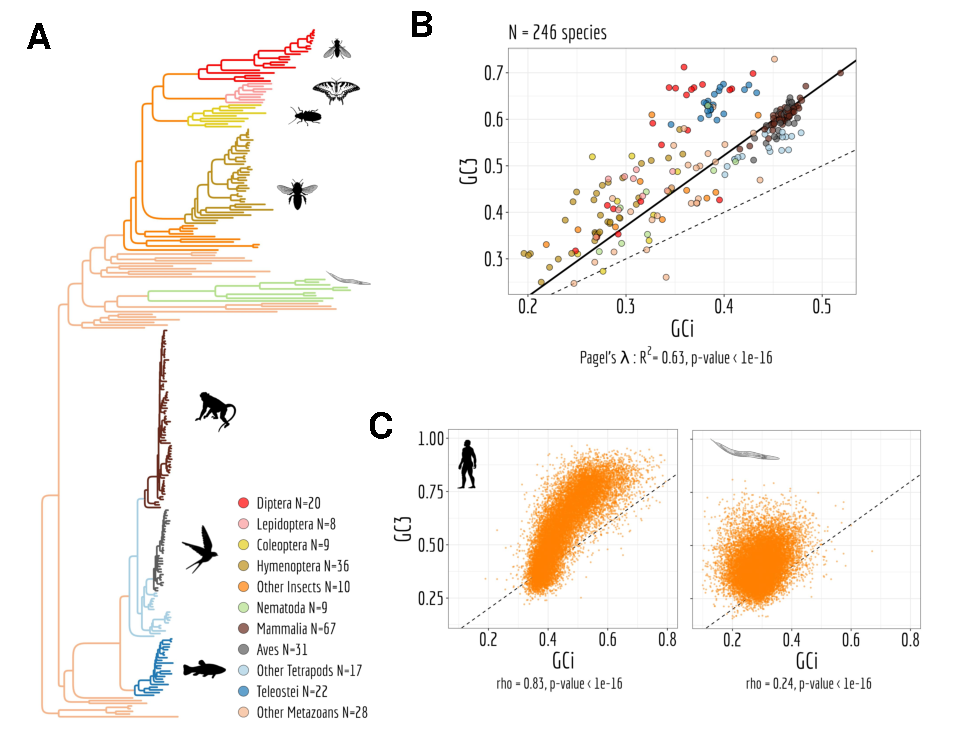
\includegraphics[width=0.9\textwidth]{Figure1.pdf}
                                                                           
    \caption[Phylogenetic distribution of the species included in the GTDrift database]{\textbf{Phylogenetic distribution of the species included in the GTDrift database.} The phylogeny was retrieved from TimeTree~\citep{kumar_timetree_2022}. Not all species studied are present (N=1,221).\newline}
    \label{fig:gtdrift1}
\end{figure}

\subsection{Collecting life history traits}
We queried several databases to acquire three specific life history traits, namely: maximum longevity, body mass, and body length. These traits were previously identified as suitable proxies for estimating the effective population size~\citep{romiguier_comparative_2014, waples_life-history_2016, figuet_life_2016, galtier_adaptive_2016, weyna_relaxation_2020}. For eusocial species, which live in colonies and have both reproductive and non-breeding individuals, we gather data on the queen of the colony. For solitary species, we collected data for females if available; otherwise, males were considered. 

We employed several distinct methodologies to screen the databases.
We initially used a manual approach to search across various sources of information, including scientific papers and databases. 

We manually searched for information on life history traits from four prominent databases, which encompass diverse taxonomic groups. The Animal Ageing and Longevity Database (AnAge)~\citep{tacutu_human_2013}, is renowned for its comprehensive collection of vertebrates, particularly mammals. The Encyclopedia of Life (\acrshort{EOL})~\citep{wilson_encyclopedia_2003, parr_encyclopedia_2014} encompasses a wide spectrum of species, prominently featuring invertebrates. The Animal Diversity Web (\acrshort{ADW})~\citep{myers_animal_2023}, is a particularly rich resource for invertebrates. The FishBase~\citep{froese_fishbase_2023} predominantly houses data on teleostei species. 
While AnAge furnishes extensive information regarding body mass and lifespan, it is lacking data pertaining to body length (\hyperref[fig:gtdrift2]{Fig. 2A,B,C}). Furthermore, as previously noted, certain databases are tailored to specific clades. For instance, in comparison to \acrshort{EOL} and \acrshort{ADW}, AnAge contains relatively fewer records for invertebrates (\hyperref[fig:gtdrift2]{Fig. 2D,E,F}). 

We then made efforts to automate the manual search procedures. The primary automated procedure involved the development of a bash script, which utilized the Latin nomenclature of the species to navigate the textual content within the research pages of the 4 databases listed above. The bash script was designed to extract sentences, words, and numerical data in proximity to keywords such as "longevity", "mass", and "weight", serving as indicators of relevant information.
Its output was then reformatted through an R script. While this approach proved effective for databases like AnAge, EOL, and FishBase, its applicability to the \acrshort{ADW} database was limited due to the manner in which information is embedded within textual paragraphs.
Consequently, we employed an alternative method for the \acrshort{ADW} database, involving machine learning and Natural Language Processing Question-Answering techniques. We obtained a trained model named "tinyroberta-squad2" from huggingface.co~\cite{wolf_huggingfaces_2020}. This model was used to answer questions related to specific attributes, such as `what is the body length ?'; `what is the body mass ?'; `what is the longevity ?'. Each question retrieved a pool of 100 potential answers derived from the database's textual content, ranked by their predictive scores provided by the model. 

We implemented an iterative selection process to identify the highest predicted answer containing relevant units and numeric values. To avoid redundancy, the selected answer was then removed from the text, and the process was repeated up to 10 times. The entire procedure was implemented in a Python script. We processed the script's output to restructure the obtained results.

Discrepancies between the manual approach and the other two methodologies were further re-investigated manually and corrected as needed after a further re-reading of the text. As a result, the curated dataset that we share reflects our highest level of confidence.

In total, our data collection effort resulted in the acquisition of life history traits for 969 metazoan species.

\begin{figure}[t]   
         \centering
        \includegraphics[width=\textwidth]{Figure2.pdf}
                                                                           
    \caption[Representation of life history traits retrieved from diverse data sources]{\textbf{Representation of life history traits retrieved from diverse data sources.} Depiction of data origins for lifespan (\textbf{A}), body length (\textbf{B}), and body mass (\textbf{C}). Additionally, distribution of species and their respective clades with at least one recorded life history trait in \acrshort{ADW} (\textbf{D}), \acrshort{EOL} (\textbf{E}), and AnAge (\textbf{F}).\newline}
    \label{fig:gtdrift2}
\end{figure}

\subsection{Acquisition of the reference genome sequence and annotations}
Using the sra-tools software, we performed an automated identification of the reference genome for each species. Subsequently, we downloaded the annotation data in GFF format, the nucleotide coding sequences in FASTA format, and the peptide sequences in FASTA format from the NCBI database~\citep{sayers_database_2022}.

\subsection{$dN/dS$ pipeline}
We developed a pipeline to estimate the rate of non-synonymous substitutions divided by the synonymous substitutions rate (${dN}/{dS}$), representing the frequency at which non-synonymous changes occur relative to synonymous ones. Since non-synonymous substitutions are commonly perceived as errors, ${dN}/{dS}$ serves as a measure of the rate of erroneous substitutions per neutral substitution. This ratio is directly dependant of \acrshort{Ne}~as it is jointly determined by the distribution of selection coefficient of new mutations (s) and the magnitude of genetic drift as defined by \acrshort{Ne}~\citep{yang_synonymous_1998, nielsen_estimating_2003}. The transcriptome-wide ${dN}/{dS}$ is expected to rise over prolonged periods of small \acrshort{Ne}~due to the increasing number of slightly deleterious mutations reaching fixation~\citep{ohta_nearly_1992, galtier_adaptive_2016}.

Estimating the ${dN}/{dS}$ necessitates the annotation of genes shared across all species, their evolutionary history depicted by a phylogenetic tree, and finally a comparative analysis of site evolution to derive the ${dN}/{dS}$ ratio.

\subsubsection{BUSCO genes identification}
We used the \acrshort{BUSCO} v.3.1.0 software to identify single-copy orthologous genes within three datasets selected from OrthoDB v9~\citep{zdobnov_orthodb_2017}: eukaryota (N=303 genes), embryophyta (N=1,440 genes) and metazoan (N=978 genes) sourced from \acrshort{BUSCO}v3~\citep{waterhouse_busco_2018, seppey_busco_2019, manni_busco_2021}. The search was performed against the longest annotated protein sequences \textit{per} gene within each genome.

\subsubsection{Phylogenetic tree reconstruction}
Due to the considerable time and resource demands associated with phylogenetic inference for large numbers of species, we employed a strategy in which the analysis was partitioned by clades. 
On initial releases of the database, which did not encompass all current species, we performed 3 comparable and independent analyses that rely on the three \acrshort{BUSCO} datasets, corresponding to the following lineages: eukaryota, embryophyta and metazoa.
For each \acrshort{BUSCO} dataset, we selected a subset of species that matched the lineage of interest from the available database records at the time of analysis. All of these selected species underwent transcriptomic analyses (see \nameref{sec:transcriptomic_analyses}). We then collected the longest corresponding proteins identified in each species for each \acrshort{BUSCO} gene family. We removed proteins for which the amino acid sequence provided with the annotations did not perfectly correspond to the translation of the corresponding coding sequences. We then aligned the resulting sets of protein-coding sequences for each \acrshort{BUSCO} gene, using the codon alignment option in PRANK v.170427~\citep{loytynoja_phylogeny-aware_2008}. We translated the codon alignments into protein alignments using the R package seqinr~\citep{charif_seqinr_2007}.

A filter was applied to retain only genes for which enough species have been detected (85\% of the analyzed species), reducing the eukaryota set to 126 genes (embryophyta N=387 genes, metazoa N=731 genes). Then, species were removed from the analysis if they had less than 80\% of the studied genes, reducing the number of studied species from 336 to 279 for the eukaryota \acrshort{BUSCO} dataset (embryophyta 93 to 80 species, metazoa 293 to 257 species).

To infer the phylogenetic tree rapidly, we sub-sampled the resulting multiple alignments, selecting alignments with the highest number of species (eukaryota N=25 genes, embryophyta N=77 genes, metazoa N=146 genes). We then concatenated these alignments and kept sites that were aligned in most of the analyzed species (see information provided in the supplementary archive for more details).
The final alignment for the eukaryota \acrshort{BUSCO} dataset included 279 taxa (embryophyta N=80 species, metazoa N=257 species) taxa and 600 sites (embryophyta N=700 sites, metazoa N=3,000 sites). We used RAxML-NG~\citep{kozlov_raxml-ng_2019}, to infer the species phylogeny on these final alignments. RAxML was set to perform one model \textit{per} gene with a fixed empirical substitution matrix (LG), empirical amino acid frequencies from alignment (F) and 8 discrete GAMMA categories (G8). These parameters were specified in a partition file with one line \textit{per} \acrshort{BUSCO} gene multiple alignment. The analysis generated at least 10 starting trees. The best-scoring topology was kept as the final \acrshort{ML} tree and 10 bootstrap replicates have been generated.

The phylogenetic trees were rooted using as a reference source the TimeTree phylogeny, which synthesizes data from numerous published studies, despite its incomplete representation of all species~\citep{kumar_timetree_2022}.

To encompass a broader spectrum of the species included in our latest database release, the one published here, we also reconstructed phylogenetic trees \textit{per} clade. To do this, we divided the full set of metazoan species in 9 groups (Hymenoptera, Diptera grouped with Lepidoptera under the superorder Mecopterida, Nematoda, other insects, Aves, Mammalia, Teleostei, other vertebrates, and finally other invertebrates). We used as a basis for the analysis 73 highly prevalent metazoan \acrshort{BUSCO} genes among the 731 genes preselected in the metazoa analysis. We applied the protocol described above to each individual clade. The resulting clade-specific trees were merged using outgroup species as a reference point to construct the complete metazoan phylogenetic tree.

\subsubsection{${dN}/{dS}$ computation}
We computed ${dN}/{dS}$ ratios for \acrshort{BUSCO} gene families that were present in at least 85 percent of the species under investigation. We conducted four independent analyses. We first analyzed each of the three \acrshort{BUSCO} gene sets: eukaryota (N=126 genes), embryophyta (N=387 genes), metazoa (N=731 genes). We also performed an analysis `\textit{per} clade', as explained above for the phylogenetic tree reconstruction, using the same 731 genes preselected in the metazoa analysis. Codon alignments obtained using PRANK~\citep{loytynoja_phylogeny-aware_2008} served as the basis for this estimation. To manage the computational memory demands during the substitution rate estimation step, we segmented the sequence alignments into clusters. Following the approach recommended by~\citet{bolivar_gc-biased_2019}, these clusters were defined based on the average \acrshort{GC3} content across species, in order to group genes with similar parameters. We then concatenated the alignments within each group, obtaining alignments that were 200 \acrshort{kb} long on average. This process yielded 13 groups for eukaryota (15 for embryophyta and 73 for metazoa).
We used bio++ v.3.0.0 libraries~\citep{dutheil_non-homogeneous_2008, gueguen_bio_2013, bolivar_gc-biased_2019} to estimate the ${dN}/{dS}$ on each branch of the phylogenetic tree, for each concatenated alignment.

In a first step, we used an homogeneous codon model implemented in bppml to infer the most likely branch lengths, codon frequencies at the root, and substitution model parameters. We used YN98 (F3X4)~\citep{yang_synonymous_1998} substitution model, which allows for different nucleotide content dynamics across codon positions. In a second step, we used the MapNH substitution mapping method to count synonymous and non-synonymous substitutions~\citep{dutheil_efficient_2012, gueguen_unbiased_2018}. 
We defined dN as the total number of non-synonymous substitutions divided by the total number of non-synonymous mutational opportunities, both summed across concatenated alignments, for each branch of the phylogenetic tree. Likewise, we defined dS as the total number of synonymous substitutions divided by the total number of synonymous mutational opportunities, both summed across concatenated alignments. The \textit{per}-species ${dN}/{dS}$ corresponds to the ratio between dN and dS, on the terminal branches of the phylogenetic tree. We also provide the dN and dS values for each branch within the phylogenetic trees.

For the `\textit{per} clade' approach, the results pertaining to distinct clades were combined in a single table.

\subsection{Transcriptomic analyses}
\label{sec:transcriptomic_analyses}
We developed a pipeline facilitating the detection of alternative splicing events within genes. This process entails the selection of RNA-seq data, subsequent alignment to the reference genome, and the identification of splicing events through the recognition of introns. Utilizing the aligned transcriptomic data, we computed gene expression levels across each sample.

\subsubsection{Selection of the RNA-seq samples}
To extract RNA-seq data, we queried the Short Read Archive (SRA) database for samples where the library source was `TRANSCRIPTOMIC' and the library strategy was `RNA-seq'. 

For perfect comparability of transcriptome data among species, we would need to have the same representation of individual tissues, developmental stages \textit{etc.} for each species, with data generated with the same protocol by the same person. However, such data exist only for limited sets of species (\textit{e.g.},~\citet{cardoso-moreira_gene_2019}). 
Here, we decided not to filter the RNA-seq samples on criteria pertaining to sample origin or experimental protocols, mainly because the relevant information is not always provided in sufficient detail in the SRA database~\citep{leinonen_sequence_2011}. Moreover, depending on the clade, the biological sample of origin can vary from "whole body" in insects, to specific tissues or cell types in mammals. Thus, perfectly comparable sample collections are difficult to obtain across such a broad phylogenetic scale.


Rather than filtering samples on these criteria prior to inclusion in the database, in GTDrift we provide users with the information collected from SRA for all \acrshort{RNA}-seq samples. This information includes the library type, the date of extraction and the name of the laboratory that performed the experiment (see \nameref{sec:datarecords}).

After evaluating the amount of \acrshort{RNA}-seq data that is needed to evaluate global alternative splicing patterns for each species (see below), we decided to include a maximum of 50 \acrshort{RNA}-seq samples \textit{per} species in GTDrift. We included more than 50 samples for 150 species (43 embryophyta, 107 metazoa), for which we performed more detailed analyses, considering various tissues or developmental stages.

In the current version of GTDrift, the \acrshort{RNA}-seq dataset encompasses a total of 491 distinct species, including 92 plants and 399 animals. (\hyperref[fig:gtdrift3]{Fig. 3A}).

\begin{figure}[t]   
         \centering
        \includegraphics[width=0.75\textwidth]{Figure3.pdf}
                                                                           
    \caption[Species with transcriptomic data and alternative splicing estimation]{\textbf{Species with transcriptomic data and alternative splicing estimation.} (\textit{cf} Fig. 2A~\citet{benitiere_random_2024}) \textbf{A}: Taxonomic distribution of the species for which transcriptomic data was included in GTDrift. \textbf{B}: Definition of the variables used to compute the relative splicing frequency of a focal intron, compared to splice variants with a common alternative splice boundary (RAS) or compared to the unspliced form  (RANS): $\mathrm{N_s}$: number of spliced reads corresponding to the precise excision of the focal intron; $\mathrm{N_a}$: number of reads corresponding to alternative splice variants relative to this intron (\textit{i.e.} sharing only one of the two intron boundaries); $\mathrm{N_u}$: number of unspliced reads, co-linear with the genomic sequence. \textbf{C}: Definitions of the main variables used in this study. The definition of the variables corresponds to the one provided in \citet{benitiere_random_2024}.\newline}
    \label{fig:gtdrift3}
\end{figure}

\subsubsection{Indexing genomes and aligning RNA-seq data}
The RNA-seq alignment phase represents the most time-consuming stage in the pipeline (\hyperref[fig:gtdrift4]{Fig. 4}), and can extend up to one week when utilizing 16 cores for each RNA-seq dataset, particularly for larger genomes such as those of mammals.

For this step, HISAT2 version 2.1.0 was employed to align RNA-seq reads to the respective reference genomes~\citep{kim_graph-based_2019}. To enhance the sensitivity of splice junction detection, we constructed genome indexes incorporating annotated intron and exon coordinates along with genome sequences. The maximum permitted intron length was set at 2,000,000 base pairs. The processed and compressed files generated during this procedure can amass a size exceeding 20 terabytes.

We extracted intron coordinates from the HISAT2 alignments, utilizing a custom Perl script that scanned for CIGAR strings containing "N" characters, which indicate skipped regions in the reference sequence. For intron identification and quantification, we exclusively utilized uniquely mapped reads with a maximum mismatch fraction of 0.02. In the context of new intron identification, we imposed a minimum anchor length (\textit{i.e.}, part of the read that spans each of the two exons flanking a given intron) of 8 base pairs. We then quantified intron splicing frequencies by including aligned reads with a minimum anchor length of 5 base pairs. We retained predicted introns exhibiting GT-AG, GC-AG, or AT-AC splice signals and determined the intron strand based on the splice signal.

Introns were assigned to genes if at least one of their boundaries was within 1 base pair of annotated exon coordinates, combined across all isoforms for each gene. Intron assignments were limited to those that could be unambiguously associated with a single gene. Notably, we differentiated between annotated introns, present in the reference genome annotations, and unannotated introns, identified through RNA-seq data and assigned to previously annotated genes.

We identified introns situated within protein-coding regions. To do this, for each protein-coding gene, we extracted annotated start and stop codon positions across all annotated isoforms. The minimum start codon and maximum end codon positions were identified, and introns located upstream or downstream of these extreme coordinates were considered as interrupting untranslated regions.

\subsubsection{Alternative splicing variables}
\label{sec:asvariables}
For each intron, we recorded two key variables: $\mathrm{N_s}$ representing the number of reads corresponding to the precise removal of the intron (referred to as spliced reads), and $\mathrm{N_a}$ representing the count of reads supporting alternative splicing events (\textit{i.e.} spliced variants sharing only one of the two boundaries of the focal intron). Additionally, we denoted $\mathrm{N_u}$ as the count of unspliced reads that align linearly with the genomic sequence and span at least 10 base pairs on both sides of an exon-intron junction. These definitions are visually clarified in (\hyperref[fig:gtdrift3]{Fig. 3B,C}). Subsequently, we introduced the relative measurement of the target intron's abundance compared to introns with a single alternative splice boundary ($\mathrm{RAS=\frac{N_s}{N_s~+{N_a}}}$), as well as relative to unspliced reads ($\mathrm{RANS=\frac{N_s}{N_s+~\frac{N_u}{2}}}$).

To compute these ratios, we required at least 10 reads in their denominators. Thus, we computed the RAS only when ($\mathrm{N_s+N_a})\geq10$, and the RANS only when ($\mathrm{N_s+\frac{N_u}{2}})\geq10$. We divided $\mathrm{N_u}$ by 2 because unspliced reads that span the two intron boundaries likely refer to the same intron retention event. If these conditions were not met, the resulting values were designated as unavailable (NA). These ratios were computed utilizing data from all available RNA-seq samples, unless explicitly specified (\textit{e.g.} in sub-sampling analyses). Based on these ratios, we divided introns into three categories: major-isoform introns, defined as those introns that have RANS $>$ 0.5 and RAS $>$ 0.5 (these likely correspond to the introns of major isoforms~\citep{gonzalez-porta_transcriptome_2013, tress_alternative_2017, benitiere_random_2024}); minor-isoform introns, defined as those introns that have RANS $\leq$ 0.5 or RAS $\leq$ 0.5 (these introns are detected in a minority of transcripts); unclassified introns, which do not satisfy the above conditions.

\subsubsection{Gene expression estimation}
Gene expression levels were computed using Cufflinks version 2.2.1~\citep{trapnell_transcript_2010, roberts_identification_2011}, utilizing the read alignments obtained with HISAT2 for each individual RNA-seq sample. We thus evaluated gene expression levels with the Fragment \textit{Per} Kilobase of exon \textit{per} Million mapped reads (\acrshort{FPKM}) method. To determine the representative expression level of each gene, the mean \acrshort{FPKM} was calculated across all samples, taking into consideration the sequencing depth of each sample, called `weighted \acrshort{FPKM}'. We used this measure to evaluate the relationship between alternative splicing rates and gene expression levels, within each species.

\subsubsection{Estimation of the sequencing depth}
We determined for each gene the union of all annotated exon coordinates (termed here exon blocks). Using bedtools v2.25.0~\citep{quinlan_bedtools_2010}, we assessed the read coverage at each position of the exon blocks. The average exonic \textit{per}-base read coverage was subsequently computed for each gene. The sequencing depth of a given sample was evaluated through the median \textit{per}-base read coverage across \acrshort{BUSCO} (Benchmarking Universal Single-Copy Orthologs) genes.

\subsection{Data visualisation using a Shiny app}
A Shiny app available at \url{https://lbbe-shiny.univ-lyon1.fr/ShinyApp-GTDrift/} was deployed to allow users to visualize and compare the summarized data~\citep{chang_shiny_2024}. Most of the graphics shown in this paper are directly reproducible from the app. In this app, users can also visualize intra-species variables, for example comparing introns or gene characteristics. Furthermore, a specific tab is dedicated to the investigation of gene structure in relation to the splicing attributes found in the underlying database. Users can also visualize the phylogenetic tree and employ these trees for conducting Phylogenetic Generalized Least Square regression analyses.

The app is organized in several panels or "tabs" in the web page.

The tab `Inter-species graphics' facilitates the comparison of genome characteristics across different species through graphical representation. Additionally, users have the option to upload their own data in a tab-separated text format, where each species is represented in a separate row, with the variables of interest organized in columns. An example of such a tabular dataset can be found in the repository. 

The `Inter-species Axis' tab explains the variables available in the `Inter-species graphics' tab.

The `Intra-species graphics' tab permits the exploration of characteristics within a species, focusing on introns or on genes. Furthermore, users have the ability to retrieve metadata related to \acrshort{BUSCO} annotation, gene expression, or intron splicing events (see \nameref{sec:methods}).

The `Intra-species Axis' tab describes the variables featured in the `Intra-species graphics' tab.

Within the `Gene structure' tab, users can delve into the introns detected in RNA-seq alignments for a specific gene. These introns are color-coded based on various criteria, including their location within the CDS or outside of it, as well as whether they are classified as major or minor-isoform introns (see \nameref{sec:methods}).

The `Phylogenetic tree' tab facilitates the examination of phylogenetic trees used for conducting Phylogenetic Generalized Least Squares regression within the `Inter-species graphics' tab.

\subsection{Data and code availability}
All processed data that we generated and used in this study, as well as the scripts that we used to analyze the data and to generate the figures, are available at the following Zenodo DOI: \url{https://doi.org/10.5281/zenodo.10022493}. 
The database is provided on Zenodo with the DOI: \url{https://doi.org/10.5281/zenodo.10017653}.
Finally, the Shiny app is available at: \url{https://lbbe-shiny.univ-lyon1.fr/ShinyApp-GTDrift/} and on Zenodo with the DOI: \url{https://doi.org/10.5281/zenodo.10022520}.

\section{Results}
\subsection{Description of the data available in GTDrift}
\label{sec:datarecords}

In GTDrift, we provide a manageable number of compressed data tables for each species processed via our pipeline (\hyperref[fig:gtdrift4]{Fig. 4}). Tables are stored in tab-delimited text format, which makes them easy to access for users with experience in bioinformatics. They are user-friendly because of the simplicity of their contents. To access these tables, users can visit the Zenodo DOI: \url{https://doi.org/10.5281/zenodo.10017653} and select their desired data type. The data can also be easily explored through a web application written in Shiny at \url{https://lbbe-shiny.univ-lyon1.fr/ShinyApp-GTDrift/}. Data exploration is thus easily accessible even for users who do not have a background in bioinformatics. 

Our database is centered around transcriptomics data. At the time of publication, the database contained over 15,935 RNA-seq samples distributed over 491 embryophytes and metazoans (\hyperref[fig:gtdrift1]{Fig. 1}), providing gene expression and alternative splicing events data. Additionally, we have enriched the database with annotations for orthologous single-copy genes (\acrshort{BUSCO} genes) and proxies of effective population size, including the molecular evolutionary rate ${dN}/{dS}$ and life history traits such as longevity, body mass, body length. We used similar types of data in our recent publication exploring the relationship between random genetic drift and alternative splicing patterns \citep{benitiere_random_2024}. However, here we provide considerably more data, for 1,506 species compared to 53 in this publication. 

Below, we provide information on the data types that are currently available in GTDrift. 

\begin{figure}[t]   
         \centering
        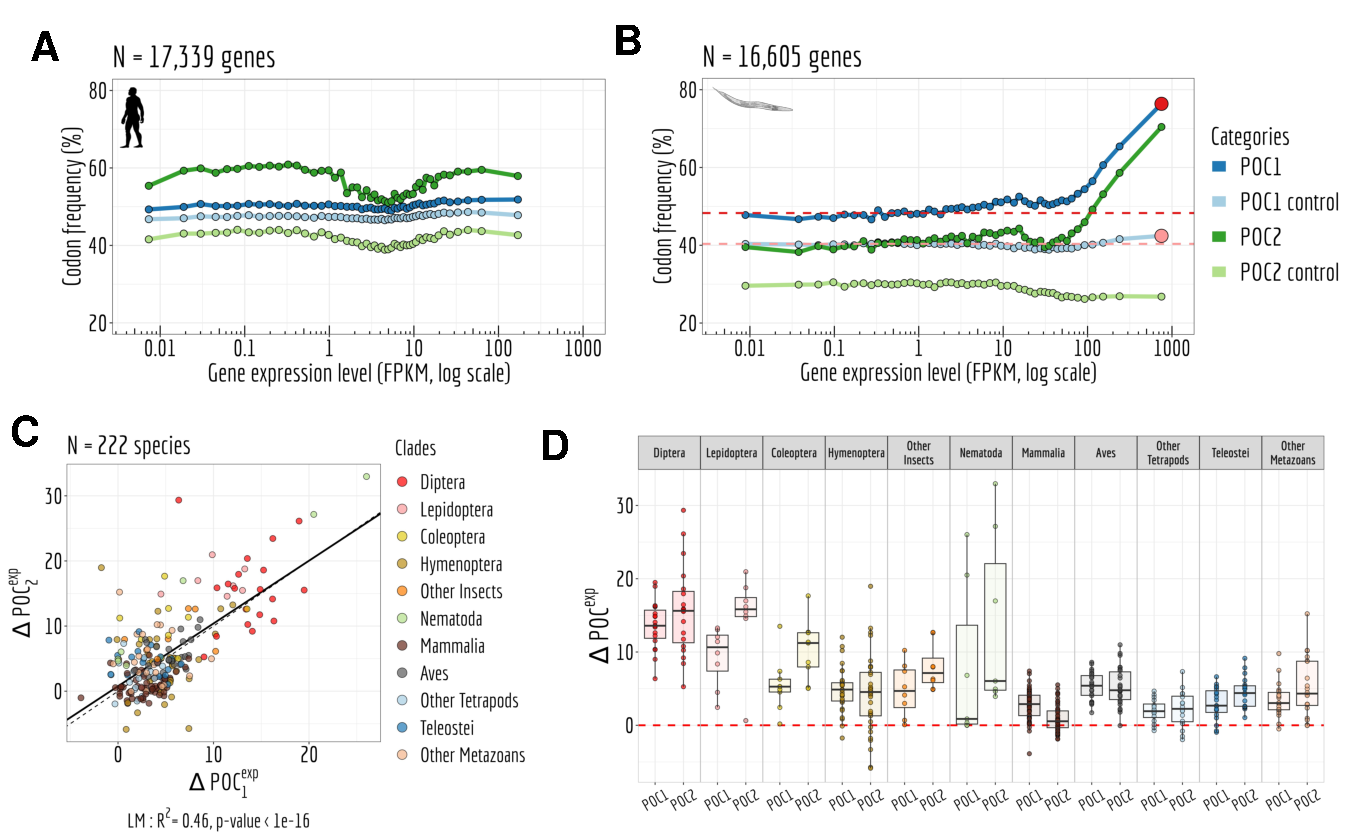
\includegraphics[width=\textwidth]{Figure4.pdf}
                                                                           
    \caption[Description of the bioinformatic analysis pipeline]{\textbf{Description of the bioinformatic analysis pipeline.} (Adapted from Supplementary Fig. 11~\citet{benitiere_random_2024}) First, we retrieved genomic sequences and annotations from the NCBI Genomes database. We aligned RNA-seq reads on the corresponding reference genomes  with HISAT2. We used these alignments to estimate various variables related to splicing patterns (see \hyperref[fig:gtdrift2]{Fig. 2}), to compute the \acrshort{AS} rate, and to estimate gene expression using Cufflinks. To compute the ${dN}/{dS}$ ratios, we first identified \acrshort{BUSCO} genes with \acrshort{BUSCO}v3 and aligned their coding sequences (CDS) using PRANK (codon model). We reconstructed a phylogenetic tree using RAxML-NG. Using bio++, we estimated ${dN}/{dS}$ along the phylogenetic tree on concatenated alignments. This pipeline was previously used in \citet{benitiere_random_2024}.\newline} 
    \label{fig:gtdrift4}
\end{figure}

\subsubsection{Life history traits}
The table labeled `life\_history\_traits.tab' comprises values pertaining to three distinct traits (longevity, body mass, and body weight), for 969 species. This table includes bibliographic references which attribute these values to each species. The species are defined by their scientific names and by the corresponding NCBI taxonomy identifier (taxID). 

\subsubsection{Protein-coding sequence evolution features}
We provide estimates of the representative ${dN}/{dS}$ ratio for most species (N=1,324 species after filtering for a sufficient number of annotated orthologous genes). The data are available in the directory `dNdS'.

We provide the phylogenetic tree of the studied species, with the ${dN}/{dS}$ ratios as branch lengths, in the Newick file format. We provide this data separately for the four approaches used to estimate the ratios ${dN}/{dS}$, using the eukaryota, embryophyta or metazoa \acrshort{BUSCO} gene sets, or a different gene set for each clade (\nameref{sec:methods}). In addition, we provide a table comprising the dN and dS values for each terminal branch of the phylogenetic tree, along with the species scientific name and NCBI taxonomy ID, for each of the four approaches.

\subsubsection{Gene expression}
In the `Transcriptomic' directory, each species is represented by a dedicated table named `by\_gene\_analysis.tab.gz'. This table contains annotated gene coordinates, the mean and median \acrshort{FPKM} (Fragments \textit{Per} Kilobase of exon \textit{per} Million mapped reads) across samples. Additionally, the table includes information about RNA-seq read coverage for exonic regions for each gene, including the total read coverage across samples. The individual gene expression data for each RNA-seq experiment can be accessed within the `RUN' directory. The data are provided in a separate directory for each SRA accession number. The file `by\_gene\_db.tab.gz' containing the exon coverage and the \acrshort{FPKM} measured for each gene corresponding in line to the previous file `by\_gene\_analysis.tab.gz'.

\subsubsection{Alternative splicing data}
For each species, we provide a summarized table named `by\_intron\_analysis.tab.gz', containing for each intron the cumulative counts of spliced reads ($\mathrm{N_s}$), the number of reads supporting alternative splicing of this introns ($\mathrm{N_a}$), and the number of unspliced reads overlapping with this intron ($\mathrm{N_u}$) detected through RNA-seq analysis (\nameref{sec:methods}). This table contains data combined across all analyzed RNA-seq samples. Detailed information for individual RNA-seq experiments can be found within the `RUN' directory, in the file `by\_intron\_db.tab.gz'. In these files, introns are listed in the same order as in the file `by\_intron\_analysis.tab.gz'.

\subsubsection{RNA-seq sample description}
In the file named `SRAruninfo.tab', we provide information extracted from the SRA database, for each RNA-seq sample. Depending on the sample, this information can include the library source, the tissue from which the sample is derived, the sex of the sampled individual, the lab that conducted the analysis, the methods used to prepare the library, \textit{etc}.

\subsubsection{BUSCO genes identification}
In the directory `BUSCO\_annotations', we provide the correspondence between NCBI gene identifiers and \acrshort{BUSCO} gene identifiers, determined for three distinct \acrshort{BUSCO} datasets: eukaryota, metazoa, and embryophyta.

\subsection{Data quality validation}
\label{sec:TechnicalValidation}
\subsubsection{Acquiring life history traits}
To facilitate the acquisition of life history traits, we have devised and shared a pipeline that uses an automatic screening technique complemented by a machine learning method.

To assess the effectiveness of the automatic screening technique that we used to extract life history traits from various databases, we conducted a comparative analysis, contrasting it with the manual methodology. We also compared it to the machine learning (ML) approach for the \acrshort{ADW} database. The screening procedure yielded accurate information with varying false positive rates depending on the source database, as follows: AnAge (98.9\% accuracy; 0\% false positive), fishbase (100\%; 0.2\%), EOL (94.5\%; 0.18\%), and \acrshort{ADW} (88\%; 5.4\%). These results highlight the utility of our screening pipeline for identifying three key life history traits across AnAge, \acrshort{EOL}, \acrshort{ADW}, and fishbase databases.

For the \acrshort{ADW} database, the \acrshort{ML} approach exhibited a slight advantage over the screening method, and its results did not completely align with those obtained through the screening approach. Specifically, for life history traits, the \acrshort{ML} approach correctly retrieved 89.7\% of the results obtained through the manual approach, while introducing a 9.2\% false positive rate.

When combining both the \acrshort{ML} approach and the screening process, we achieved a 95\% accuracy rate in identifying positive cases. However, a 7\% error rate persisted in this merged approach.

In GTDrift, we provide data corresponding to a synthesis of the three methodologies including only manually-checked values (\nameref{sec:methods}).


\subsubsection{Estimating the intensity of random drift}
As expected, a positive correlation is observed in \hyperref[fig:gtdrift5]{Fig. 5A,B} between the different life history traits, used as indirect predictors of the effective population size (\acrshort{Ne})~\citep{romiguier_comparative_2014, waples_life-history_2016, figuet_life_2016, galtier_adaptive_2016, weyna_relaxation_2020}.


\begin{figure}[t]  
         \centering
        \includegraphics[width=\textwidth]{Figure5.pdf}
                                                                           
    \caption[\Ne~proxies]{\textbf{\Ne~proxies.} \textbf{A}: Relationship between body length (cm, log scale) and longevity (days, log scale) of the organism. Each dot represents one species (colored by clade). \textbf{B}: Relationship between body length (cm, log scale) and the body weight (kg, log scale). \textbf{A,B}: Pagel's \textit{lambda} model is used to take into account the phylogenetic structure of the data in a regression model.\newline}
    \label{fig:gtdrift5}
\end{figure}

When examining the ${dN}/{dS}$ ratio across distinct time scales and using various \acrshort{BUSCO} datasets, we consistently observe comparable ${dN}/{dS}$ ratios at terminal branches. This uniformity across a range of methodological approaches highlights their concordance (\hyperref[fig:gtdrift6]{Fig. 6A,B}). 

\begin{figure}[t]   
         \centering
        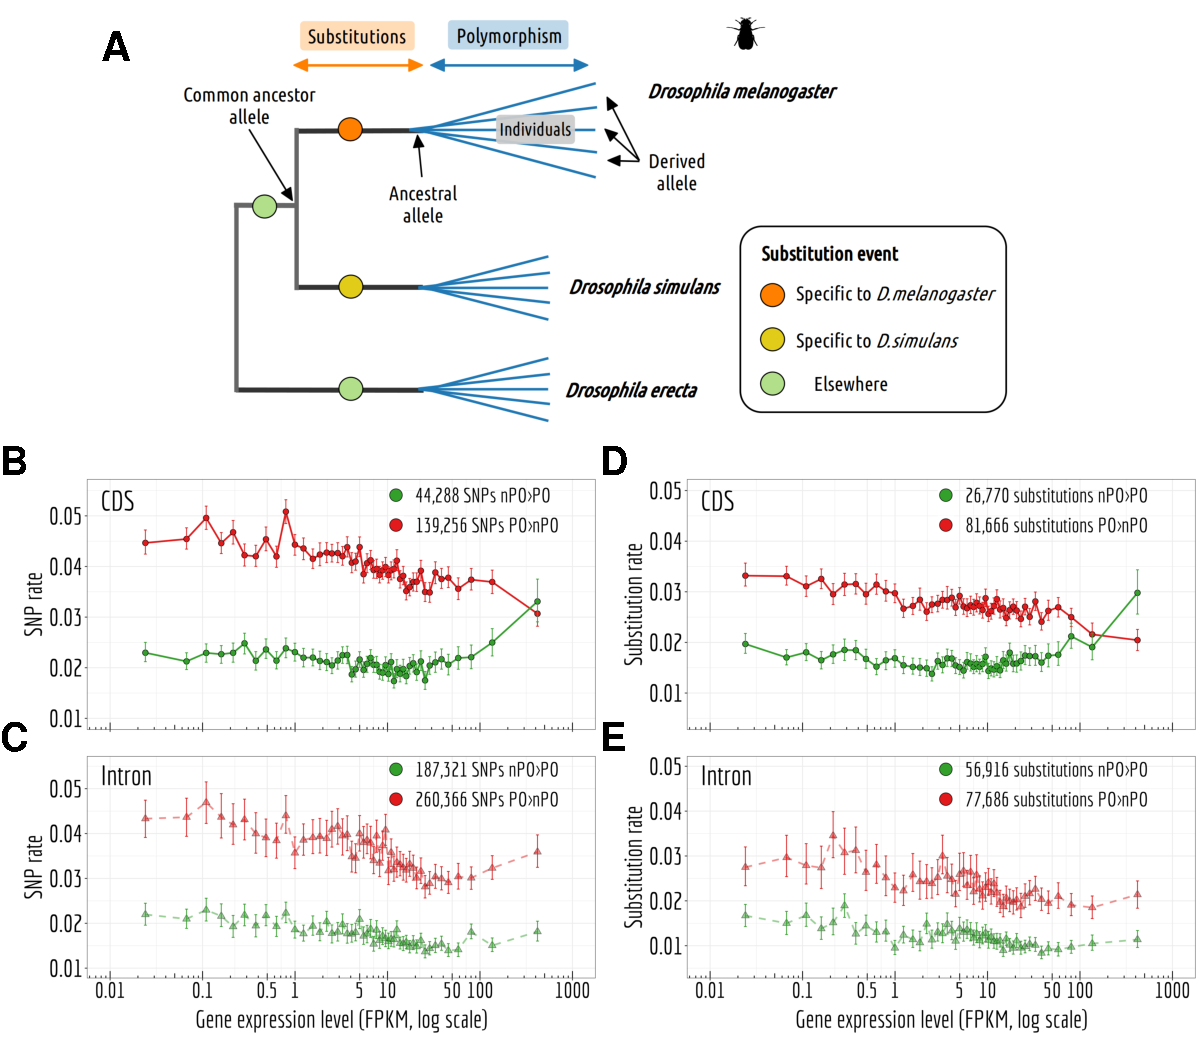
\includegraphics[width=\textwidth]{Figure6.pdf}
                                                                           
    \caption[Reproducibility of the ${dN}/{dS}$ ratio]{\textbf{Reproducibility of the ${dN}/{dS}$ ratio.} \textbf{A}: Relation between the ${dN}/{dS}$ ratio on terminal branches of the phylogenetic tree of the metazoa set compared to the ones measured in the \textit{per} clades set. \textbf{B}: Relation between the ${dN}/{dS}$ ratio on terminal branches of the phylogenetic tree of the eukaryota set compared to the ones measured in the embryophyta and the metazoa set. \textbf{A,B}: LM stands for Linear regression Model and Pagel's \textit{lambda} model is used to take into account the phylogenetic structure of the data in a regression model.\newline}
    \label{fig:gtdrift6}
\end{figure}

Furthermore, the observed ${dN}/{dS}$ ratio are significantly correlated with proxies derived from life history traits (\hyperref[fig:gtdrift7]{Fig. 7A,B}) as reported in the literature~\citep{romiguier_comparative_2014, figuet_life_2016}.

\begin{figure}[t]   
         \centering
        \includegraphics[width=0.82\textwidth]{Figure7.pdf}
                                                                           
    \caption[Interplay between \Ne~proxies]{\textbf{Interplay between \Ne~proxies.} Correlation between the ${dN}/{dS}$ ratio on terminal branches of the phylogenetic tree of the \textit{per} clade set and life history traits:  longevity (days, log scale) (\textbf{A}), body weight (kg, log scale) (\textbf{B}), body length (cm, log scale) (\textbf{C}). \textbf{A,B,C}: Pagel's \textit{lambda} model is used to take into account the phylogenetic structure of the data in a regression model.\newline}
    \label{fig:gtdrift7}
\end{figure}

\subsection{Quality of genome annotations}
To assess gene expression levels and alternative splicing patterns, the quality of genome annotations is of paramount importance. We evaluated genome annotation quality by examining the presence of \acrshort{BUSCO} genes. We note that the results depend on the \acrshort{BUSCO} dataset that is used as a starting point. When using the \acrshort{BUSCO} dataset designed for eukaryota, which comprises 303 genes, we have effectively identified nearly all single-copy orthologous genes, and this feature exhibits a high degree of homogeneity across different species (\hyperref[fig:gtdrift8]{Fig. 8}). However, the aves clade demonstrates a deficiency in the number of \acrshort{BUSCO} genes compared to the anticipated count based on \acrshort{BUSCO} expectations. This is expected given the known genome incompleteness problem for this clade, due to the presence of GC-rich chromosomes~\citep{li_novo_2022}. 

Because the eukaryota \acrshort{BUSCO} gene set is limited, we also performed gene identification for the metazoa and embryophyta \acrshort{BUSCO} datasets, leading to substantially larger collections of genes. Specifically, we detected 978 \acrshort{BUSCO} genes for the metazoa dataset and 1,440 genes for the embryophyta dataset.

\begin{figure}[t]   
         \centering
        \includegraphics[width=\textwidth]{Figure8.pdf}
                                                                           
    \caption[BUSCO genes annotation]{\textbf{\acrshort{BUSCO} genes annotation.} Proportion of \acrshort{BUSCO} genes, from the \acrshort{BUSCO} gene set eukaryota (N=303 genes), identified in each species.\newline}
    \label{fig:gtdrift8}
\end{figure}

\subsection{Spliced introns classification}
A significant body of literature has consistently reported that the majority of genes typically exhibit one predominant isoform~\citep{gonzalez-porta_transcriptome_2013, tress_alternative_2017}. This isoform is commonly termed "major isoform". Here, we aimed to assess the influence of sequencing depth on the identification of major-isoform introns, that is, those introns that belong to major isoforms (see \nameref{sec:asvariables}). Employing the model organism \textit{Drosophila melanogaster}, we randomly selected between 1 and 20 RNA-seq samples. For each subset of samples, we computed the median read coverage across the exons of \acrshort{BUSCO} genes, providing a standardized measure of transcriptome sequencing depth that can be compared across different species. Additionally, we tallied the count of introns falling into various categories (major-isoform introns, minor-isoform introns or unclassified introns - see \nameref{sec:methods}) for each subset of samples. This entire process was repeated 10 times (\hyperref[fig:gtdrift9]{Fig. 9A}).

As expected, we observed that the number of major-isoform introns that could be identified increased with greater sequencing depth until it reached a threshold of 200 read coverage \textit{per} base (\hyperref[fig:gtdrift9]{Fig. 9A}). Beyond this threshold, no additional major-isoform introns are discernible. Simultaneously, the count of unclassified introns decreased to nearly zero, indicating that introns newly detected above the 200-read coverage threshold predominantly consisted of minor-isoform introns that shared a boundary with a major intron. Indeed, the count of minor-isoform introns continued to rise steadily beyond this point.

We then assessed the proportion of annotated introns that fall within the categories defined above. Our results reveal that the majority of species exhibit well-annotated major-isoform introns, indicating the accuracy of the intron annotation (\hyperref[fig:gtdrift9]{Fig. 9B}). Additionally, as sequencing depth increases, we observed a decreasing fraction of annotated minor-isoform introns. This trend is consistent with expectations, given that higher sequencing depth expands the pool of rare variants and potential spontaneous errors that may not have been previously observed. It is important to note that there appears to be no inherent limit to this phenomenon, as the intricacies of alternative splicing machinery can give rise to unpredictable errors~\citep{benitiere_random_2024}.

\begin{figure}[t]  
         \centering
        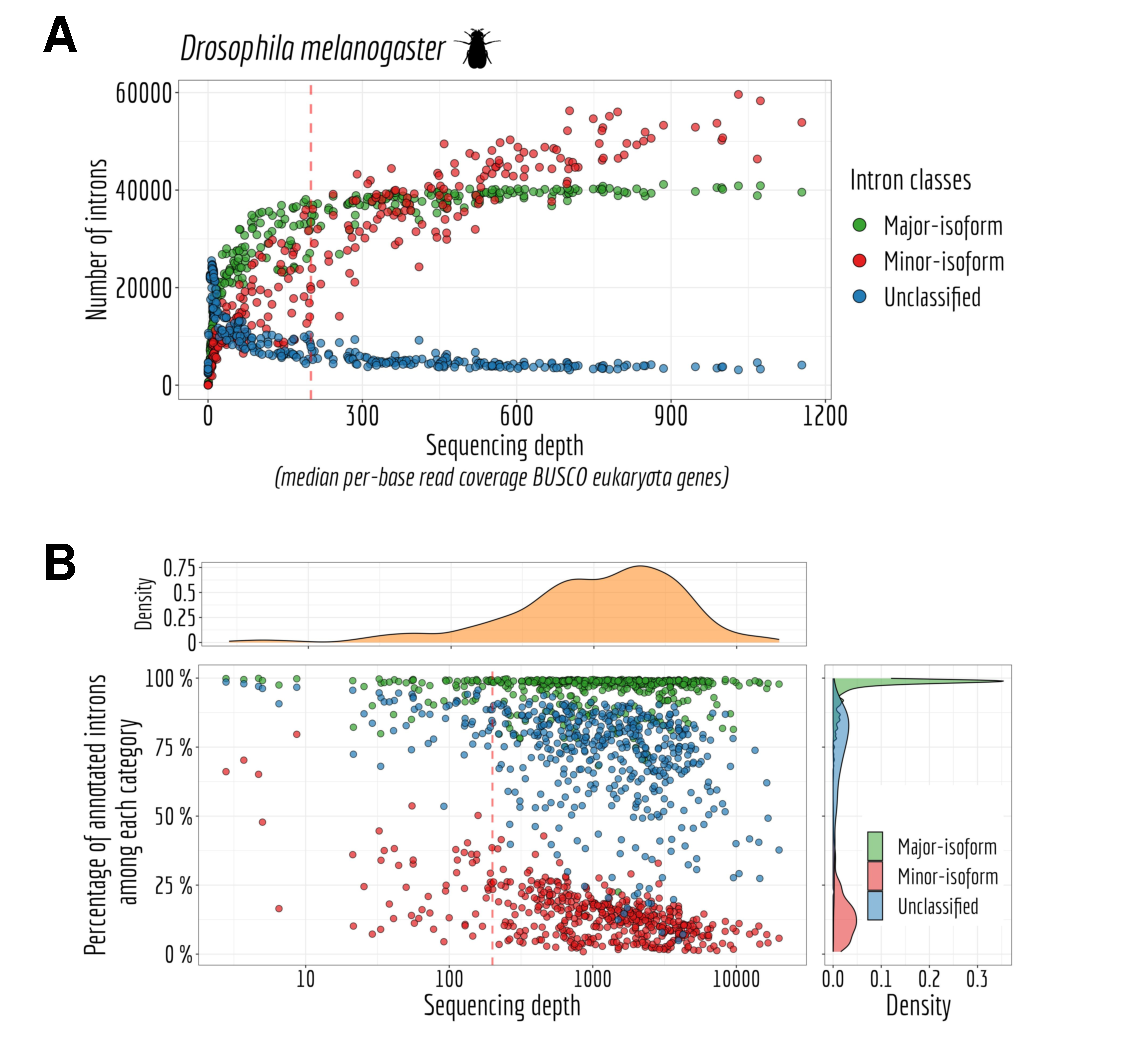
\includegraphics[width=0.9\textwidth]{Figure9.pdf}
                                                                           
    \caption[Sequencing depth impact on intron classification]{\textbf{Sequencing depth impact on intron classification.} \textbf{A}: Number of major (RANS $>$ 0.5 and RAS $>$ 0.5), minor (RANS $\geq$~5\% or RAS $\geq$~5\% ) and unclassified introns for \emph{Drosophila melanogaster}. The sequencing depth is measured by taking the median \textit{per}-base read coverage across \acrshort{BUSCO} genes from eukaryota gene set. \textbf{B}: \textit{Per} species major-isoform introns, minor-isoform introns and undetermined introns ($\mathrm{N_s})\geq10$) annotated proportion and sequencing depth measured by taking the median \textit{per}-base read coverage eukaryota \acrshort{BUSCO} genes.\newline}
    \label{fig:gtdrift9}
\end{figure}

\section{Discussion}
GTDrift is a comprehensive data resource facilitating investigations of genomic and transcriptomic characteristics alongside indicators of genetic drift intensity for distinct species. Notably, this resource offers information on life history traits, including longevity, adult body length, and body mass, for a curated set of 969 species. Additionally, it provides estimates of the ratio between the rate of non-synonymous \gls{substitution}s over synonymous \gls{substitution}s (${dN}/{dS}$) for 1,324 species.

For individual species, intron-centered alternative splicing frequencies, gene expression levels, and sequencing depth statistics have been systematically quantified and shared, encompassing more than 15,935 RNA-seq samples across 491 species. To enable cross-species comparisons, orthology predictions for conserved single-copy genes are provided, based on \acrshort{BUSCO} gene sets, encompassing a total of 1,506 eukaryotic species, including 1,413 animals and 93 green plants, along with phylogenetic trees to account for phylogenetic inertia.

The number of species per data type varies due to different limitations: availability of life history traits data; completeness of gene annotations for ${dN}/{dS}$ calculation; computational resources and availability of RNA-seq samples for transcriptomic analysis (\hyperref[fig:gtdrift4]{Fig. 4}).

These pre-processed data streamlines the work for those interested in investigating the impact of drift on biological processes across a wide range of species. All data are provided in flat files, which enable downstream computational analyses and render GTDrift mainly aimed at users with some computational skills. Nonetheless, to enhance accessibility, we have developed a user-friendly Shiny app that facilitates database exploration and allows for species-specific data downloads (available at \url{https://lbbe-shiny.univ-lyon1.fr/ShinyApp-GTDrift/}).

\subsection{Cautionary considerations in utilizing \Ne~proxies}

Users should bear in mind that the scientific community has yet to establish the most adequate proxies for effective population size. A prominent hypothesis suggests that these proxies are associated with the number of individuals (\acrshort{N}). Indeed, species with greater longevity and larger body mass tend to be less abundant within their ecological niche due to resource (mass) and spatial (length, mass) requirements~\citep{damuth_population_1981, nee_relationship_1991, white_relationships_2007}. Therefore, variations in life history traits should correspond to variations in the number of individuals (\acrshort{N}), which subsequently impact \acrshort{Ne}.

When using the ${dN}/{dS}$ ratio as a proxy for \acrshort{Ne}, rather than focusing on correlations with the population census, we evaluated the efficiency of natural selection to purge deleterious mutations. This efficiency can be represented as the product of \acrshort{Ne}~and `\acrshort{s}', which denotes the selection coefficient. The extent to which a well-estimated ${dN}/{dS}$ ratio can be considered as a proxy for \acrshort{Ne}~remains a subject of debate. Notably, when the rate of synonymous \gls{substitution}s \gls{dS} exceeds 1, it indicates a point of saturation where multiple \gls{substitution}s occur \textit{per} site, rendering dS susceptible to considerable noise due to the challenge of accurately identifying the number of \gls{substitution}s at given sites. In such cases, the dN component can often still be reliably determined. Given that non-synonymous \gls{substitution}s have a lower rate compared to synonymous ones, \gls{dN} reaches a saturation point at a later stage.

Moreover, when the evolutionary time frame is relatively short, characterized by small \gls{dS} values, the variants under examination are primarily attributed to polymorphism rather than fixed substitutions. In such cases, we are not effectively measuring substitution rates. Consequently, the discussion also revolves around determining a divergence threshold, above which we could assume that \gls{dS} and \gls{dN} predominantly represent substitutions, with minimal influence from polymorphism. In this perspective, the expanding polymorphism data could potentially serve as a means to distinguish between polymorphism and substitutions, offering a more efficient approach to investigate ${dN}/{dS}$~\citep{mugal_why_2014}.

Overall, we found that the various \acrshort{Ne}~proxies were significantly correlated, even when accounting for the underlying phylogenetic structure. Thus, our dataset, which encompasses information on \gls{dN} and \gls{dS} across all branches of the phylogenetic trees, holds the potential to estimate the long-term effective population size (\acrshort{Ne}) and its interaction with life history traits over time.

\subsection{Comparing transcriptomic data}
In our study, we have identified \acrshort{BUSCO} genes for the eukaryota, metazoa, or embryophyta \acrshort{BUSCO} reference gene sets. To ensure meaningful comparisons between species with a sufficient number of detected \acrshort{BUSCO} genes, we evaluated the median RNA-seq coverage of these \acrshort{BUSCO} genes. As demonstrated in \nameref{sec:TechnicalValidation}, the median \textit{per}-base read exonic RNA-seq coverage of \acrshort{BUSCO} genes is a good indicator of the power to detect alternative splicing patterns. We believe that, for the inclusion of additional species, an examination of the RNA-seq read coverage on \acrshort{BUSCO} genes is needed to ensure that we could identify major-isoform introns and analyze alternative splicing patterns.

Additionally, it is essential to assess the completeness of the genome and of the annotation, which can be estimated based on the number of identified \acrshort{BUSCO} genes. Some species may have a limited number of well-annotated \acrshort{BUSCO} genes, or global gene duplications may result in the presence of two copies of a \acrshort{BUSCO} gene, which no longer qualifies as a single copy gene.

Our RNA-seq description table offers users access to information collected from the Sequence Read Archive (SRA) for the RNA-seq datasets under study. This table enables users to filter and select RNA-seq data that align with their specific research needs. Users can tailor their selection based on factors such as sex, tissue, or protocol. Depending on the research question that is asked, it may be important to extract and analyse RNA-seq samples that were generated for the same biological conditions. We provide this information so that GTDrift users are able to filter the data as needed. 

To facilitate cross-species comparisons, especially in the context of alternative splicing and gene expression, users can make use of \acrshort{BUSCO} gene sets, which should exhibit consistent expression patterns, functionality, and evolutionary constraints across diverse species. However, users should thoroughly validate this assumption and proceed with vigilance.

\subsection{Conclusion}
In conclusion, we are confident that the GTDrift database can be a valuable resource for studies aiming to investigate the relationship between the intensity of genetic drift, genomic and transcriptomic characteristics.

\subsection*{Acknowledgements}
We thank Loïc Guille for his contribution to an initial pilot study, Tristan Lefébure for insightful discussions and Laurent Guéguen for his help on ${dN}/{dS}$ analyses. 
Computational analyses were performed using the computing facilities of the CC LBBE/PRABI and the Core Cluster of the Institut Français de Bioinformatique (IFB) (ANR-11-INBS-0013).
Silhouette images of taxonomic Families originate from PhyloPic developed and maintained by Mike Keesey available at \url{https://www.phylopic.org/}.

\subsection*{Author contributions statement}
F.B. conceived the pipeline and conducted the analyses. F.B. and A.N. drafted the manuscript. All authors reviewed the manuscript. 

\subsection*{Funding}
This work was funded by the French National Research Agency (ANR-20-CE02-0008-01 "NeGA" and ANR-17-CE12-0019-01 "LncEvoSys").

\subsection*{Competing interests}
The authors declare no conflicts of interest.

    
    \thispagestyle{empty}
    
    \chapter[Random genetic drift sets an upper limit on mRNA splicing accuracy in metazoans]{Random genetic drift sets an upper limit on mRNA splicing accuracy in metazoans}
    \label{chap:AlternativeSplicing}

    \vspace*{30pt}

    The second objective of my thesis is to explore the impact of random genetic drift on alternative splicing in metazoans. Indeed, most eukaryotic genes undergo alternative splicing (AS), but the overall functional significance of this process remains a controversial issue. It has been noticed that the complexity of organisms (assayed by the number of distinct cell types) correlates positively with their genome-wide AS rate. This has been interpreted as evidence that AS plays an important role in adaptive evolution by increasing the functional repertoires of genomes. \\
    
    However, this observation also fits with a totally opposite interpretation: given that ‘complex’ organisms tend to have small effective population sizes (\acrshort{Ne}), they are expected to be more affected by genetic drift, and hence more prone to accumulate deleterious mutations that decrease splicing accuracy. Thus, according to this “drift barrier” theory, the elevated AS rate in complex organisms might simply result from a higher splicing error rate.  \\
    
    To test this hypothesis, based on a pre-release of GTDrift, we analyzed 3,496 transcriptome sequencing samples to quantify \acrshort{AS} in 53 metazoan species spanning a wide range of \acrshort{Ne}~values. Our results led to a published paper where we showed a negative correlation between \acrshort{Ne}~proxies and the genome-wide \acrshort{AS} rates among species, consistent with the drift barrier hypothesis. This pattern is dominated by low abundance isoforms, which represent the vast majority of the splice variant repertoire. We show that these low abundance isoforms are depleted in functional \acrshort{AS} events, and most likely correspond to errors. Conversely, the \acrshort{AS} rate of abundant isoforms, which are relatively enriched in functional \acrshort{AS} events, tends to be lower in more complex species. \\
    
    All these observations are consistent with the hypothesis that variation in \acrshort{AS} rates across metazoans reflects the limits set by drift on the capacity of selection to prevent gene expression errors.

    \newpage
    
    \begin{tikzpicture}[scale=0.4,transform shape,remember picture,overlay]
    \hypersetup{hidelinks}
    \node[anchor=north west,yshift=20pt,xshift=700pt]
    { \href{https://doi.org/10.24072/pci.evolbiol.100642}{\includegraphics[height=35mm]{chap6-Alternative Splicing/figures/badge_PCI_Evol_Biol.png}} } ;
    \end{tikzpicture}

    \begin{tikzpicture}[scale=0.4,transform shape,remember picture,overlay]
    \hypersetup{hidelinks}
    \node[anchor=north west,yshift=60pt,xshift=810pt]
    { \href{https://elifesciences.org/articles/93629}{\includegraphics[height=35mm]{chap6-Alternative Splicing/figures/badge_elife.png}} } ;
    \end{tikzpicture}
    
    
    \vspace*{10pt}
    
    \begin{center}
    \Large{\textbf{Random genetic drift sets an upper limit on mRNA splicing accuracy in metazoans}} \\
    \end{center}
    
    \begin{flushleft}
    \oneline{\large \textbf{{Florian Bénitière}$^{1,2}$ \orcidlink{0000-0001-7773-3542}, {Anamaria Necsulea$^{1}$ \orcidlink{0000-0001-9861-7698}}, {Laurent Duret}$^{1}$ \orcidlink{0000-0003-2836-3463}}}
    
    \small
    \begin{center}
    $^{1}$Laboratoire de Biométrie et Biologie Évolutive, UMR CNRS 5558 LBBE, Université Claude Bernard Lyon 1, Villeurbanne, France\\
    $^{2}$Laboratoire d'Ecologie des Hydrosystèmes Naturels et Anthropisés, UMR CNRS 5023 LEHNA, Université Claude Bernard Lyon 1, Villeurbanne, France\\
    \end{center}
    \end{flushleft}

    {\hypersetup{linkcolor=GREYDARK}\minitoc\newpage}
    
\graphicspath{{chap6-Alternative Splicing/figures/}}

\section{Introduction}
Eukaryotic protein-coding genes are interrupted by introns, which have to be excised from the primary transcript to produce functional mRNAs that can be translated into proteins. The removal of introns from primary transcripts can lead to the production of diverse mRNAs, \textit{via} the differential use of splice sites. This process of alternative splicing (AS) is widespread in eukaryotes~\citep{chen_correcting_2014}, but its 'raison d'être' (adaptive or not) remains elusive. Numerous studies have shown that some \acrshort{AS} events are functional, \textit{i.e.} that they play a beneficial role for the fitness of organisms, either by allowing the production of distinct protein isoforms~\citep{graveley_alternative_2001} or by regulating gene expression post-transcriptionally~\citep{mcglincy_alternative_2008, hamid_emerging_2014}. However, other \acrshort{AS} events are undoubtedly not functional. Like any biological machinery, the spliceosome occasionally makes errors, leading to the production of aberrant mRNAs, which represent a waste of resources and are therefore deleterious for the fitness of the organisms~\citep{hsu_spliceosomes_2009, gout_large-scale_2013}. The splicing error rate at a given intron is expected to depend both on the efficiency of the spliceosome and on the intrinsic quality of its splice signals. The information required in cis for the removal of each intron resides in 20 to 40 nucleotide sites, located within the intron or its flanking exons~\citep{lynch_origins_2006}. Besides the two splice sites that are essential for the splicing reaction (almost always GT for the donor and AG for the acceptor), all other signals tolerate some sequence flexibility. Population genetics principles state that the ability of selection to promote beneficial mutations or eliminate deleterious mutations depends on the intensity of selection (s) relative to the power of random genetic drift (defined by the effective population size, \acrshort{Ne}): if the selection coefficient is sufficiently weak relative to drift ($|$\textit{N}$_{\text{e}} s| \ll 1 $), alleles behave as if they are effectively neutral. Thus, random drift sets an upper limit on the capacity of selection to prevent the fixation of alleles that are sub-optimal~\citep{kimura_mutation_1963, ohta_slightly_1973}. This so-called “drift barrier”~\citep{lynch_frailty_2007} is expected to affect the efficiency of all cellular processes, including splicing. Hence, species with low \acrshort{Ne}~should be more prone to make splicing errors than species with high \acrshort{Ne}.

The extent to which \acrshort{AS} events correspond to functional isoforms or to errors is a contentious issue~\citep{bhuiyan_systematic_2018, tress_most_2017, blencowe_relationship_2017, tress_alternative_2017}. In humans, the set of transcripts produced by a given gene generally consists of one major transcript (the ‘major isoform‘), which encodes a functional protein, and of multiple minor isoforms (splice variants), present in relatively low abundance, and whose coding sequence is frequently interrupted by premature termination codons (PTCs)~\citep{tress_alternative_2017,gonzalez-porta_transcriptome_2013}. Ultimately, less than 1\% of human splice variants lead to the production of a detectable amount of protein~\citep{abascal_alternatively_2015}. Furthermore, comparison with closely related species showed that \acrshort{AS} patterns evolve very rapidly~\citep{barbosa-morais_evolutionary_2012,merkin_evolutionary_2012} and that alternative splice sites present little evidence of selective constraints~\citep{pickrell_noisy_2010}. All these observations are consistent with the hypothesis that a vast majority of splice variants observed in human transcriptomes simply correspond to erroneous transcripts~\citep{pickrell_noisy_2010}. However, some authors argue that a large fraction of \acrshort{AS} events might in fact contribute to regulating gene expression. Indeed, PTC-containing splice variants are recognized and degraded by the non-sense mediated decay (NMD) machinery. Thus, \acrshort{AS} can be coupled with NMD to modulate gene expression at the post-transcriptional level~\citep{mcglincy_alternative_2008,hamid_emerging_2014}. This AS-NMD regulatory process does not involve the production of proteins and does not necessarily imply strong evolutionary constraints on splice sites. Thus, based on these observations, it is difficult to firmly refute selectionist or non-adaptive models.

The analysis of transcriptomes from various eukaryotic species showed substantial variation in \acrshort{AS} rates across lineages, with the highest rate in primates~\citep{barbosa-morais_evolutionary_2012,chen_correcting_2014, mazin_alternative_2021}. Interestingly, the genome-wide average \acrshort{AS} level was found to correlate positively with the complexity of organisms (approximated by the number of cell types)~\citep{chen_correcting_2014}. This correlation was considered as evidence that \acrshort{AS} contributed to the evolution of complex organisms by increasing the functional repertoire of their genomes~\citep{chen_correcting_2014}. This pattern is often presented as an argument supporting the importance of \acrshort{AS} in adaptation~\citep{verta_role_2022,singh_importance_2022, wright_alternative_2022}. However, this correlation is also compatible with a totally opposite hypothesis. Indeed, eukaryotic species with the highest level of complexity correspond to multi-cellular organisms with relatively large body size, which tend to have small effective population sizes (\acrshort{Ne})~\citep{lynch_origins_2003, figuet_life_2016}. Thus, the higher \acrshort{AS} rate observed in ‘complex’ organisms might simply reflect an increased rate of splicing errors, resulting from the effect of the drift barrier on the quality of splice signals~\citep{bush_alternative_2017}.

To assess this hypothesis and evaluate the impact of genetic drift on alternative splicing patterns, we quantified \acrshort{AS} rates in 53 metazoan species, covering a wide range of \acrshort{Ne}~values, and for which high-depth transcriptome sequencing data were available. We show that the genome-wide average \acrshort{AS} rate correlates negatively with \acrshort{Ne}, in agreement with the drift barrier hypothesis. This pattern is mainly driven by low abundance isoforms, which represent the vast majority of splice variants and most likely correspond to errors. Conversely, the \acrshort{AS} rate of abundant splice variants, which are enriched in functional \acrshort{AS} events, show the opposite trend. These results support the hypothesis that the drift barrier sets an upper limit on the capacity of selection to minimize splicing errors.

\section{Results}

\subsection{Genomic and transcriptomic data collection}\label{sec:sampling_species}
To analyze variation in \acrshort{AS} rates across metazoans, we examined a collection of 69 species for which transcriptome sequencing (RNA-seq) data, genome assemblies, and gene annotations were available in public databases. We focused on vertebrates and insects, the two metazoan clades that were the best represented in public databases when we initiated this project. To be able to compare average \acrshort{AS} rates across species, we needed to control for several possible sources of biases. First, given that \acrshort{AS} rates vary across genes~\citep{saudemont_fitness_2017}, we had to analyze a common set of orthologous genes. For this purpose, we extracted from the \acrshort{BUSCO} database~\citep{seppey_busco_2019} a reference set of single-copy orthologous genes shared across metazoans (N=978 genes), and searched for their homologues in each species in our dataset. We retained for further analyses those species for which at least 80\% of the \acrshort{BUSCO} metazoan gene set could be identified (N=67 species; see \nameref{sec:MaterialsMethodsAS}). Second, we had to ensure that RNA-seq read coverage was sufficiently high in each species to detect splicing variants. Indeed, to be able to detect \acrshort{AS} at a given intron, it is necessary to analyze a minimal number of sequencing reads encompassing this intron (we used a threshold of N=10 reads). To assess the impact of sequencing depth on \acrshort{AS} detection, we conducted a pilot analysis with two species (\textit{Homo sapiens} and \textit{Drosophila melanogaster}) for which hundreds of RNA-seq samples are available. This analysis (detailed in \hyperref[supp_fig:AS1]{Appendix Fig. A.1}) revealed that \acrshort{AS} rate estimates are very noisy when sequencing depth is limited, but that they converge when sequencing is high enough. We therefore kept for further analysis those species for which the median read coverage across exonic regions of \acrshort{BUSCO} genes was above 200 (\hyperref[supp_fig:AS1]{Appendix Fig. A.1}). Our final dataset thus consisted of 53 species (15 vertebrates and 38 insects; \hyperref[fig:AS1]{Fig. 1A}), and of 3,496 RNA-seq samples (66 \textit{per} species on average). In these species, the number of analyzable annotated introns (\textit{i.e.} encompassed by at least 10 reads) among \acrshort{BUSCO} genes ranges from 2,032 to 10,981 (which represents 88.6\% to 99.6\% of their annotated introns; \hyperref[table:1]{Appendix Tab. A.1}). It should be noted that analyzed samples originate from diverse sources; however, they are very homogenous in terms of sequencing technology (99\% of RNA-seq samples sequenced with Illumina platforms; refer to \verb|Data10-supp.tab| in the Zenodo data repository).


\subsection{Proxies for the effective population size (\Ne)}\label{sec:LHT_Ne}
Effective population sizes (\acrshort{Ne}) can in principle be inferred from levels of genetic polymorphism. However, population genetics data are lacking for most of the species in our dataset. We therefore used two life history traits that were previously proposed as proxies of \acrshort{Ne}~in metazoans~\citep{waples_life-history_2016,weyna_relaxation_2020, figuet_life_2016}: body length and longevity (\nameref{sec:MaterialsMethodsAS}; \hyperref[table:2]{Appendix Tab. A.2}). An additional proxy for \acrshort{Ne}~can be obtained by studying the intensity of purifying selection acting on protein sequences, through the ${dN}/{dS}$ ratio~\citep{kryazhimskiy_population_2008}. To evaluate this ratio, we aligned 922 \acrshort{BUSCO} genes, reconstructed the phylogenetic tree of the 53 species (\hyperref[fig:AS1]{Fig. 1A}) and computed the ${dN}/{dS}$ ratio along each terminal branch (\nameref{sec:MaterialsMethodsAS}).

\begin{figure}[t]   
    \begin{center}                                                                       
        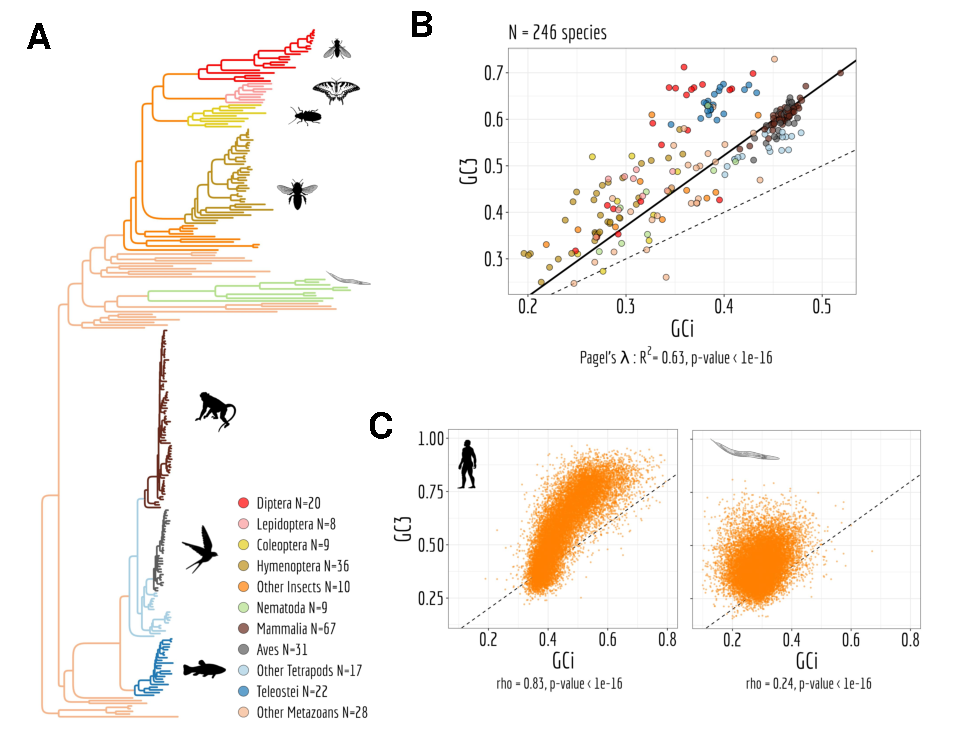
\includegraphics[width=\textwidth] {Figure1.pdf}
    \end{center}                                                                       
    \caption[Species phylogeny and \Ne~proxies]{\textbf{Species phylogeny and \acrshort{Ne} proxies.} \textbf{A}: Phylogenetic tree of the 53 studied species (15 vertebrates and 38 insects). \textbf{B}: Relationship between body length (cm, log scale) and longevity (days, log scale) of the organism. Each dot represents one species (colored by clade, as in the species tree in panel A). \textbf{C}: Relationship between longevity (days, log scale) and the ${dN}/{dS}$ ratio on terminal branches of the phylogenetic tree (\nameref{sec:MaterialsMethodsAS}).
   \textbf{B,C}: PGLS stands for Phylogenetic Generalized Least Squared regression, which takes into account phylogenetic inertia (\nameref{sec:MaterialsMethodsAS}).
    \newline}
    \label{fig:AS1}
\end{figure}

We note that these three proxies provide ”inverse” estimates of \acrshort{Ne}, meaning that species with high longevity, large body length and/or elevated ${dN}/{dS}$ values tend to have low \acrshort{Ne}~values. As expected, these different proxies of \acrshort{Ne}~are positively correlated with each other (p $<$ 1x$10^{-3}$, \hyperref[fig:AS1]{Fig. 1B,C}). We note however that these correlations are not very strong. It thus seems likely that none of these proxies provides a perfect estimate of \acrshort{Ne}. To take phylogenetic inertia into account, all cross-species correlations presented here were computed using Phylogenetic Generalized Least Squared (PGLS) regression~\citep{freckleton_phylogenetic_2002}.

\subsection{Alternative splicing rates are negatively correlated with \Ne~proxies}
\label{sec:SVR_Ne}
To quantify AS rates, we mapped RNA-seq data of each species on the corresponding reference genome assembly. We detected sequencing reads indicative of a splicing event (hereafter termed ‘spliced reads’), and inferred the corresponding intron boundaries. We were thus able to validate the coordinates of annotated introns and to detect new introns, not present in the annotations. For each intron detected in RNA-seq data, we counted the number of spliced reads matching with its two boundaries ($\mathrm{N_s}$) or sharing only one of its boundaries ($\mathrm{N_a}$), as well as the number of unspliced reads covering its boundaries ($\mathrm{N_u}$) (\hyperref[fig:AS2]{Fig. 2A}). We then computed the relative abundance of this spliced isoform compared to other transcripts with alternative splice boundaries ($\mathrm{RAS=\frac{N_s}{N_s~+~{N_a}}}$) or compared to unspliced transcripts ($\mathrm{RANS=\frac{N_s}{N_s~+~\frac{N_u}{2}}}$).


To limit measurement noise, we only considered introns for which both RAS and RANS could be computed based on at least 10 reads (\nameref{sec:MaterialsMethodsAS}). In all species, both RAS and RANS metrics show clearly bimodal distributions (\hyperref[fig:AS2]{Fig. 2B,C}): the first peak (mode $<$ 5\%) corresponds to ‘minor-isoform introns’, whose splicing occurs only in a minority of transcripts of a given gene, whereas the second one (mode $>$ 95\%) corresponds to the introns of major isoforms. It has been previously shown that in humans, for most genes, one single transcript largely dominates over other isoforms~\citep{tress_alternative_2017, gonzalez-porta_transcriptome_2013}. Our observations indicate that this pattern is generalized across metazoans. For the rest of our analyses, we computed the rate of alternative splicing with respect to introns of the major isoform. We will hereafter use the term ‘splice variant’ (\acrshort{SV}) to refer to those splicing events that are detected in a minority of transcripts (\textit{i.e.} with RAS $\leq$ 0.5 or RANS $\leq$ 0.5; see \hyperref[fig:AS2]{Fig. 2E} for a definition of the main variables used in this study).

\begin{figure}[htp]   
    \begin{center}                                                                       
        \includegraphics[width=0.82\textwidth] {Figure2.pdf}
    \end{center}                                                                       
    \caption[Distinguishing major and minor introns and measuring the rate of alternative splicing.]{\textbf{Distinguishing major and minor-isoform introns and measuring the rate of alternative splicing.}
    
  \textbf{A}: Definition of the variables used to compute the relative abundance of a spliced isoform compared to other transcripts with alternative splice boundaries (RAS) or compared to unspliced transcripts (RANS): $\mathrm{N_s}$: number of spliced reads corresponding to the precise excision of the focal intron; $\mathrm{N_a}$: number of reads corresponding to alternative splice variants relative to this intron (\textit{i.e.} sharing only one of the two intron boundaries); $\mathrm{N_u}$: number of unspliced reads, co-linear with the genomic sequence. \textbf{B,C} Histograms representing the distribution of RAS and RANS values (divided into 5\% bins), for protein-coding gene introns. Each line represents one species. Two representative species are colored: \textit{Drosophila melanogaster} (red), \textit{Homo sapiens} (brown). \textbf{D}: Description of the variables used to compute the AS rate of a given a major-isoform intron, and the 'minor-isoform intron relative abundance' (MIRA) of each of its splice variants (\acrshort{SV}s): $\mathrm{N^M}$: number of spliced reads corresponding to the excision of the major-isoform intron; $\mathrm{N_i^m}$: number of spliced reads corresponding to the excision of a minor-isoform intron (i); $\mathrm{N^m}$: total number of spliced reads corresponding to the excision of minor-isoform introns. \textbf{E}: Definitions of the main variables used in this study.\newline}
    \label{fig:AS2}
\end{figure}


We focused our analyses on major-isoform introns interrupting protein-coding regions (\textit{i.e.} we excluded introns located within UTRs, \nameref{sec:MaterialsMethodsAS}). In vertebrates, each \acrshort{BUSCO} gene contains on average 8.4 major-isoform introns (\hyperref[table:1]{Appendix Tab. A.1}). The intron density is more variable among insect clades, ranging from 2.8 major-isoform introns \textit{per} \acrshort{BUSCO} gene in Diptera to 6.1 in Blattodea. As expected, most major-isoform introns have GT/AG splice sites (99.1\% on average across species), and only a small fraction have boundaries that do not match the canonical U2-introns splice sites (0.8\% GC/AG and 0.1\% AT/AC). The fraction of non-canonical splice sites is slightly higher among minor-isoform introns (2.8\% GC/AG and 0.3\% AT/AC). This might reflect a higher prevalence of U12-type introns but might also be caused by the presence of some false positives in the set of minor-isoform introns. In any case, the difference in splice signal usage between minor and major-isoform introns is small, which indicates that the vast majority of detected minor-isoform introns correspond to \textit{bona fide} splicing events.


The proportion of major-isoform introns for which AS has been detected (\textit{i.e.} with $\mathrm{N_a}$ $>$ 0) ranges from 16.8\% to 95.7\% depending on the species (\hyperref[table:1]{Appendix Tab. A.1}). This metric is however not very meaningful because it directly reflects differences in sequencing depth across species (the higher the sequencing effort, the higher the probability to detect a rare \acrshort{SV}, \hyperref[supp_fig:AS2]{Appendix Fig. A.2}). To allow a comparison across taxa, we computed the AS rate of introns, normalized by sequencing depth ($\mathrm{AS=\frac{N^m}{N^M~+~N^m}}$, \nameref{sec:MaterialsMethodsAS}; \hyperref[fig:AS2]{Fig. 2D}). The average AS rate for \acrshort{BUSCO} genes varies by a factor of 5 among species, from 0.8\% in \textit{Drosophila grimshawi} (Diptera) to 3.8\% in \textit{Megachile rotundata} (Hymenoptera) (3.4\% in humans). Interestingly, the average AS rates of \acrshort{BUSCO} gene introns are significantly correlated with the three proxies of \acrshort{Ne}: species longevity (\hyperref[fig:AS3]{Fig. 3A}), body length and the ${dN}/{dS}$ ratio (\hyperref[supp_fig:AS3]{Supplementary Fig. 3A,B}). These correlations are positive, which implies that AS rates tend to increase when \acrshort{Ne}~decreases. It is noteworthy that despite the fact that these proxies are not strongly correlated with each other (\hyperref[fig:AS1]{Fig. 1B,C}), they all show similar relationships with AS rates. It should be stressed that these correlations were estimated using the PGLS method to account for phylogenetic inertia (and they remain significant when analyzing insects and vertebrates separately, \hyperref[supp_fig:AS4]{Appendix Fig. A.4}). Thus, these observations are consistent with the hypothesis that \acrshort{Ne}~has an impact on the evolution of AS rate.


One limitation of our analyses is that we used heterogeneous sources of transcriptomic data. To obtain enough sequencing depth, we combined for each species many RNA-seq samples, irrespective of their origin (whole body, or specific tissues or organs, in adults or embryos, etc.). It is known that genome-wide average AS rates vary according to tissues or developmental stages~\citep{barbosa-morais_evolutionary_2012,mazin_alternative_2021}, and according to environmental conditions~\citep{john_regulation_2021}. To explore how this might have affected our results, we repeated our analyses using a recently published dataset that aimed to compare transcriptomes across seven organs, sampled at several developmental stages in seven species (six mammals, one bird)~\citep{cardoso-moreira_gene_2019}. In agreement with previous reports~\citep{mazin_alternative_2021}, our analysis of \acrshort{BUSCO} genes revealed substantial differences in AS rates among organs, with consistent patterns of variation across species. For instance, in all species, testes and brain tissues show higher AS rates than liver and kidney (\hyperref[fig:AS3]{Fig. 3B}). However, the variation in AS rate among organs in each species is limited compared to differences between species. Specifically, in an ANOVA analysis performed on the average AS rate across \acrshort{BUSCO} gene introns, with the species and the organ of origin as explanatory variables, the species factor explained$~$89\% of the total variance, while the organ factor explained only$~$9\%. Among insects, we found only one species (\textit{Dendroctonus ponderosae}) for which RNA-seq samples were available from multiple tissues. Here again, the variance in AS rate among tissues was limited compared to inter-species variability (\hyperref[supp_fig:AS5]{Appendix Fig. A.5}). Thus, despite the variability that can be introduced by the heterogeneity of RNA-seq samples, the relationship between AS rate and longevity remains detectable among these seven species (\hyperref[fig:AS3]{Fig. 3B}). 

\begin{figure}[t]   
    \begin{center}                                                                       
        \includegraphics[width=\textwidth] {Figure3.pdf}
    \end{center}                                                                       
    \caption[The rate of alternative splicing correlates with life history traits across metazoans.]{\textbf{The rate of alternative splicing correlates with life history traits across metazoans.}
    
  \textbf{A}: Relationship between the \textit{per} intron average AS rate of an organism and its longevity (days, log scale). \textbf{B}: Variation in average AS rate across seven organs (brain, cerebellum, heart, liver, kidney, testis and ovary) among seven vertebrate species (RNA-seq data from~\citet{cardoso-moreira_gene_2019}). AS rates are computed on major-isoform introns from \acrshort{BUSCO} genes (\nameref{sec:MaterialsMethodsAS}).\newline}
    \label{fig:AS3}
\end{figure}


\subsection{Functional vs. non-functional alternative splicing}\label{sec:SVrare}
The negative correlation observed between \acrshort{Ne}~and alternative splicing rates is consistent with the hypothesis that differences in AS rates across species are driven by variation in the rate of splicing errors (drift barrier model). This does not exclude however that functional splicing variants might also contribute to AS rate variation across species. To evaluate this point, we selected a subset of \acrshort{SV}s that are enriched in functional AS events. To do this, we reasoned that selective pressure against the waste of resources should maintain splicing errors at a low rate (as low as permitted by the drift barrier), whereas functional \acrshort{SV}s are expected to represent a sizeable fraction of the transcripts expressed by a given gene, at least in some specific conditions (cell type, developmental stage…). Thus, functional \acrshort{SV}s are expected to be enriched among abundant \acrshort{SV}s compared to rare \acrshort{SV}s.


To assess this prediction, we analyzed the proportion of \acrshort{SV}s that preserve the reading frame according to their abundance relative to the major isoform. For this, we focused on minor-isoform introns that share a boundary with one major-isoform intron and that have their other boundary at less than 30 bp from the major splice site (either in the flanking exon or within the major-isoform intron). We determined whether the distance between the minor-isoform intron boundary and the major-isoform intron boundary was a multiple of 3. We computed the abundance of each minor isoform, relative to the corresponding major isoform, with the following formula:\\
$\mathrm{Minor~intron~relative~abundance~MIRA_i=\frac{N_i^m}{N^M~+~N^m}}$ (see \hyperref[fig:AS2]{Fig. 2D}).


We divided minor-isoform introns into 5\% bins according to their MIRA and computed for each bin the proportion of minor-isoform introns that maintain the reading frame of the major isoform (\hyperref[fig:AS4]{Fig. 4A}). In all species, we observe that this proportion varies according to the abundance of splice variants, with two distinct regimes (\hyperref[fig:AS4]{Fig. 4A}). First, for MIRA values above~5\%, the proportion of frame-preserving variants correlates positively with MIRA, reaching up to 60\%-70\% for the most abundant isoforms. Second, for MIRA values below 1\%, the proportion of frame-preserving variants does not covary with MIRA, and fluctuates around 30 to 40\%, close to the random expectation (33\%). The excess of frame-preserving variants among the most abundant isoforms implies that a substantial fraction of them is under constraint to encode functional protein isoforms. This fraction varies from 0\% for MIRA values below 1\%, to 50\% for isoforms with the highest MIRA values. It should be noted that these estimates correspond to a lower bound, since it is possible that some frame-shifting splice variants are functional. Nevertheless, these observations clearly indicate that the subset of \acrshort{SV}s with MIRA values $>$ 5\% (hereafter referred to as ‘abundant \acrshort{SV}s’) is strongly enriched in functional isoforms relative to other \acrshort{SV}s (MIRA $\leq$ 5\%, hereafter referred to as ‘rare \acrshort{SV}s’). Of note, the subset of rare \acrshort{SV}s represents the vast majority of the \acrshort{SV} repertoire (from 62.4\% to 96.9\% depending on the species; \hyperref[table:1]{Appendix Tab. A.1}). Thus, the positive correlation between AS rate and longevity reported above (\hyperref[fig:AS3]{Fig. 3A}) is mainly driven by the set of introns with a low AS rate (\hyperref[fig:AS4]{Fig. 4C}). Interestingly, introns with high AS rate (enriched in functional \acrshort{SV}s) show an opposite trend (\hyperref[fig:AS4]{Fig. 4D}), and they display a lower proportion of frame-preserving \acrshort{SV}s in vertebrates than in dipterans (\hyperref[fig:AS4]{Fig. 4B}). This is the opposite of what would have been expected if functional \acrshort{SV}s were more prevalent in complex organisms.

\begin{figure}[t]   
    \begin{center}                                                                       
        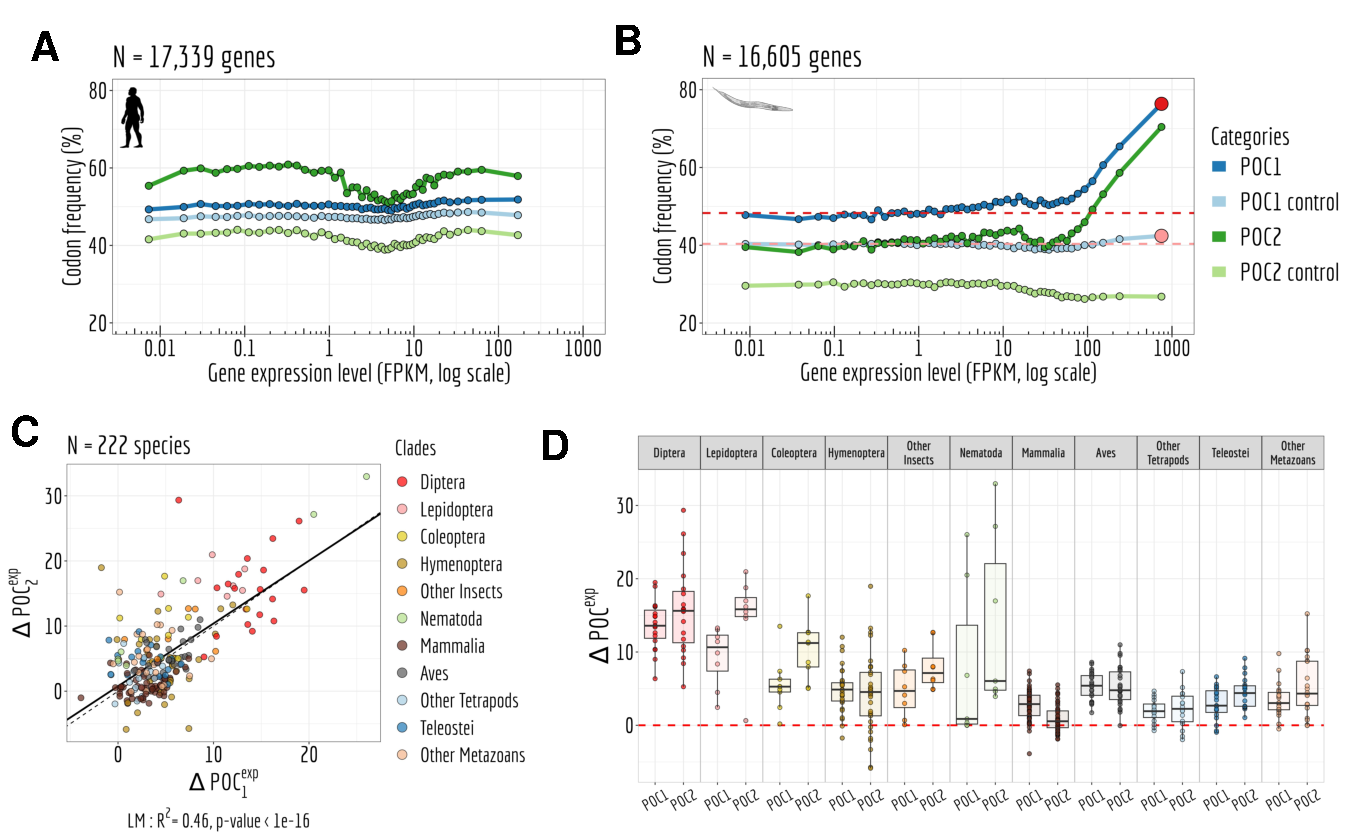
\includegraphics[width=0.8\textwidth] {Figure4.pdf}
    \end{center}                                                                       
    \caption[Variation in AS rate across metazoans: distinguishing abundant splice variants (enriched in functional variants) from rare splice variants]{\textbf{Variation in AS rate across metazoans: distinguishing abundant splice variants (enriched in functional variants) from rare splice variants.} \textbf{A}: Frame-preserving isoforms are strongly enriched among abundant splice variants (\acrshort{SV}s). For each species, \acrshort{SV}s were classified into 20 equal-size bins according to their abundance relative to the major isoform (MIRA, see \nameref{sec:MaterialsMethodsAS}), and the proportion of frame-preserving \acrshort{SV}s was computed for each bin. Each line represents one species. Three representative species are colored: red: \textit{Drosophila melanogaster}, brown: \textit{Homo sapiens}, yellow: \textit{Apis mellifera}. We used a threshold MIRA value of 5\% to define ‘abundant’ vs. ‘rare’ \acrshort{SV}s. \textbf{B}: Proportion of frame-preserving \acrshort{SV}s among abundant \acrshort{SV}s across metazoans. Each dot represents one species. All annotated protein-coding genes are used in the analysis. \textbf{C,D}: Relationship between the average \textit{per} intron AS rate of an organism and its longevity (days, log scale). Only \acrshort{BUSCO} genes are used in the analysis. \textbf{C}: Low-AS major-isoform introns (\textit{i.e.} major-isoform introns that do not have any abundant \acrshort{SV}), \textbf{D}: High-AS major-isoform introns (\textit{i.e.} major-isoform introns having at least one abundant \acrshort{SV}).\newline}
    \label{fig:AS4}
\end{figure}

\subsection{Investigating selective pressures on minor splice sites}
A complementary approach to assess the functionality of AS events consists in investigating signatures of selective constraints on splice sites. For this, we used polymorphism data from \textit{Drosophila melanogaster} and \textit{Homo sapiens} to measure single-nucleotide polymorphism (SNP) density at major and minor splice sites, considering separately rare and abundant \acrshort{SV}s. We focused on the first two and last two bases of each intron (consensus sequences GT, AG), which represent the most constrained sites within splice signals. We studied minor-isoform introns that share one splice site with a major-isoform intron and we measured SNP density at the corresponding major and minor splice sites. To account for constraints acting on coding regions, we considered separately minor splice sites that were located in an exon or in an intron of the major isoform. As negative controls, we selected AG or GT dinucleotides that were unlikely to correspond to alternative splice sites (\hyperref[fig:AS5]{Fig.~ 5}, \nameref{sec:MaterialsMethodsAS}). Furthermore, for \textit{Homo sapiens} we controlled for the presence of hypermutable \gls{CpG} dinucleotides~\citep{tomso_sequence_2003} (\hyperref[supp_fig:AS6]{Appendix Fig. A.6}, \nameref{sec:MaterialsMethodsAS}). 


\begin{figure}[t]   
    \centering                                                                                    
        \includegraphics[width=0.8\textwidth] {Figure5.pdf}                             
    \caption[Variation in selective constraints on alternative splice signals from rare and abundant SVs]{\textbf{Variation in selective constraints on alternative splice signals from rare and abundant SVs.}
For each minor-isoform intron sharing one boundary with a major-isoform intron, we measured the SNP density at its minor splice site (red), and at the corresponding major splice site (green). We distinguished minor splice sites that are located in an exon or in an intron of the major isoform. As a control (blue), we selected AG or GT dinucleotides that are unlikely to correspond to alternative splice sites, namely: AG dinucleotides located toward the end of the upstream exon or the beginning of the intron (unlikely to correspond to a genuine acceptor site), and GT dinucleotides located toward the beginning of the downstream exon or the end of the intron (unlikely to correspond to a donor site). To increase the sample size, we analyzed data from all annotated protein-coding genes (and not only the \acrshort{BUSCO} gene set). The number of sites studied is shown at the top of each bar. Error bars represent the 95\% confidence interval of the proportion of polymorphic sites (proportion test). \textbf{A,B}: SNP density in \textit{Drosophila melanogaster} (polymorphism data from 205 inbred lines derived from natural populations, N=3,963,397 SNPs \citep{huang_natural_2014, mackay_drosophila_2012}). \textbf{C,D}: SNP density in \textit{Homo sapiens} (polymorphism data from 2,504 individuals, N=80,868,061 SNPs \citep{auton_global_2015}). We excluded dinucleotides affected by \gls{CpG} hypermutability (\nameref{sec:MaterialsMethodsAS}, see \hyperref[supp_fig:AS6]{Appendix Fig. A.6} for \gls{CpG} sites). \textbf{A,C}: Abundant \acrshort{SV}s (MIRA $>$ 5\%). \textbf{B,D}: Rare \acrshort{SV}s (MIRA $\leq$ 5\%).\newline}
    \label{fig:AS5}
\end{figure}



\begin{figure}[t]   
    \centering                                                                                
        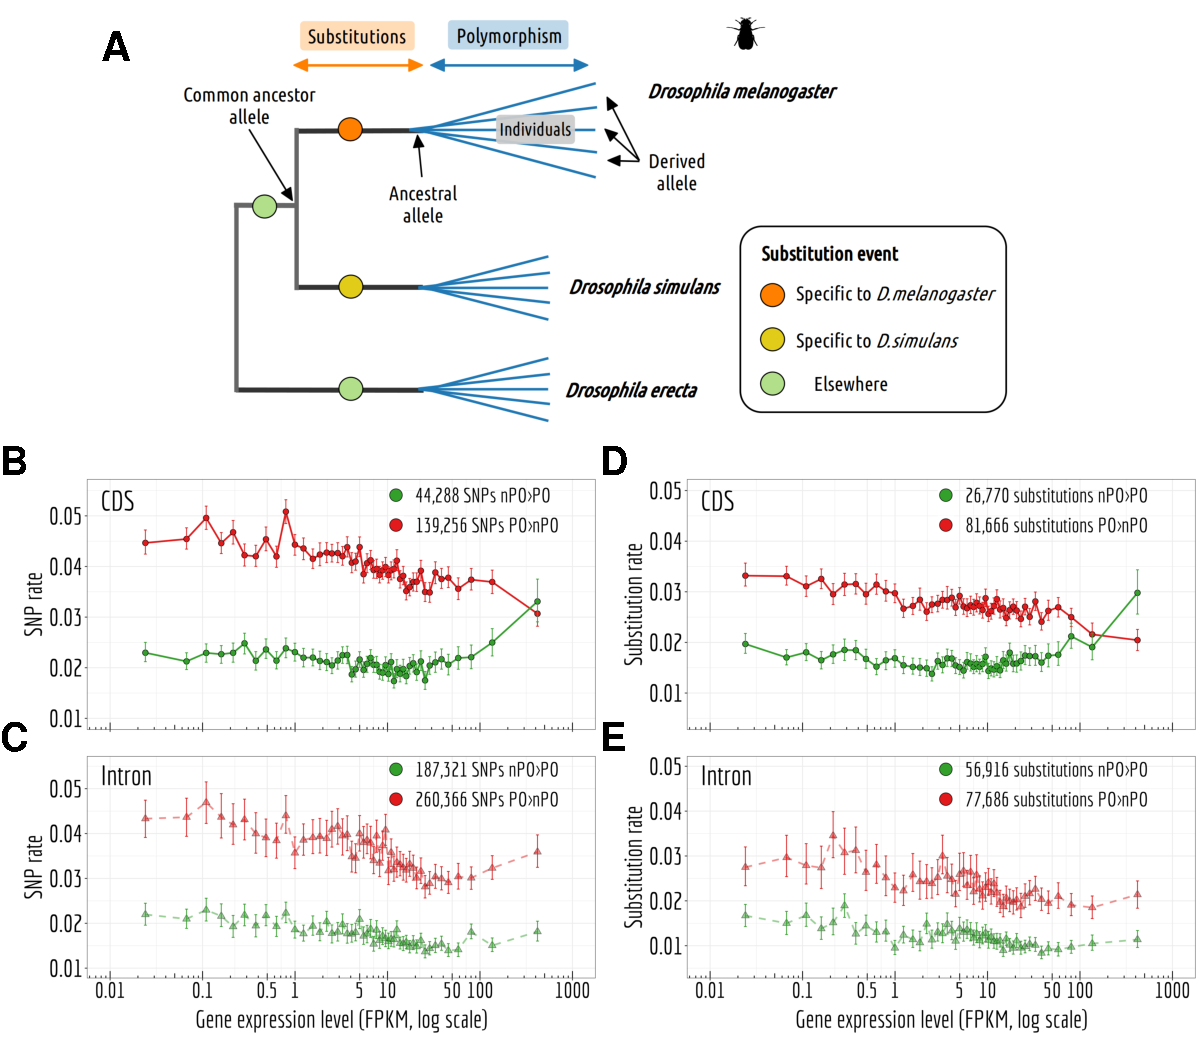
\includegraphics[width=0.8\textwidth] {Figure6.pdf}                                                           
    \caption[Relationship between AS rate and gene expression level]{\textbf{Relationship between AS rate and gene expression level.} For each species, we selected major-isoform introns with a sufficient sequencing depth to have a precise measure of their AS rate ($\mathrm{N_s+N_a}\geq100$). We divided major-isoform introns into 5\% bins according to their gene expression level and computed the correlation between the average AS rate and median expression level across the 20 bins. To increase sample size, these analyses were based on all annotated protein-coding genes (and not only the \acrshort{BUSCO} gene set). \textbf{A}: Distribution of Pearson correlation coefficients (R) between the AS rate and expression level observed in the 53 metazoans. The vertical dashed lines indicates the thresholds under and above which correlations are significant (\textit{i.e.} p-value $<$ 0.05). \textbf{B}: Distribution of Pearson correlation coefficients computed on the subsets of low-AS major-isoform introns  (\textit{i.e.} after excluding major-isoform introns with abundant \acrshort{SV}s). \textbf{C,D}: Two representative species illustrating the negative relation between the average AS rate of low-AS major-isoform introns and the expression level of their gene. Error bars represent the standard error of the mean. \textbf{C}: N=127,599 low-AS major-isoform introns from \textit{Homo sapiens}, \textbf{D}: N=31,357 low-AS major-isoform introns from \textit{Drosophila melanogaster}.\newline}
    \label{fig:AS6}
\end{figure}


For both species, the lowest SNP density is observed at major splice signals, which reflects the strong selective constraints on these sites (\hyperref[fig:AS5]{Fig. 5}). In \textit{Drosophila melanogaster}, there is also a strong signature of selection on minor splice signals of abundant \acrshort{SV}s: both in introns and in exons, the SNP density at minor splice signals of abundant \acrshort{SV}s is much lower than in corresponding controls (from -37\% to -74\%, \hyperref[fig:AS5]{Fig. 5A}) and than in minor splice signals of rare \acrshort{SV}s (from -38\% to -71\%, \hyperref[fig:AS5]{Fig. 5B}). This observation confirms that abundant \acrshort{SV}s are strongly enriched in functional variants compared to rare \acrshort{SV}s. In \textit{Homo sapiens}, patterns of SNP density showed little evidence of selective constraints on minor splice sites, irrespective of the abundance of \acrshort{SV}s (\hyperref[fig:AS5]{Fig. 5C,D}): minor acceptor splice sites (AG) located within the major-isoform intron show a weak but significant SNP deficit relative to corresponding control sites (p-value $<$ 1x$10^{-5}$), but other categories of minor splice sites do not show any sign of selective constraints. The fact that the signature of selection on minor splice signals is much weaker in humans compared to \textit{Drosophila} is indicative of a lower prevalence of functional variants, even among abundant \acrshort{SV}s. This observation is therefore in total contradiction with the adaptive hypothesis (more functional alternative splicing in complex organisms).


\subsection{The splicing rate of rare SVs is negatively correlated with gene expression levels}
The above analyses are consistent with the hypothesis that the vast majority of rare \acrshort{SV}s correspond to erroneous transcripts, and that changes in \acrshort{Ne}~contribute to variation in AS rate across taxa by shifting the selection-mutation-drift balance. If true, then this model predicts that the erroneous AS rate should also vary among genes, according to their expression level. Indeed, it has been shown that the selective pressure on splicing accuracy is stronger on highly expressed genes~\citep{saudemont_fitness_2017}. This reflects the fact that for a given splicing error rate, the waste of resources (both in terms of metabolic cost and of futile mobilization of cellular machineries) increases with gene expression level~\citep{saudemont_fitness_2017,xiong_drift_2017}. Thus, the selection-mutation-drift balance should lead to a negative correlation between gene expression level and the rate of splicing errors. To test this prediction, we focused on low-AS major-isoform introns, \textit{i.e.} introns that are unlikely to have functional \acrshort{SV}s. For each species, we considered all major-isoform introns with a sufficient sequencing depth to have a precise measure of their AS rate ($\mathrm{N_s+N_a}\geq100$). The selected subset represents 38.1\% to 86.7\% of major-isoform introns of each species (median=70.9\%). Introns were then divided into 20 bins of equal size, according to the expression level of the corresponding genes. For each species, we computed the Pearson correlation between the average AS rate and the average expression level across bins. We observed a negative correlation between AS rates and gene expression levels in 52 out of the 53 species (significant with p $<$ 0.05, in 48/53 species; \hyperref[fig:AS6]{Fig. 6A}; two representative examples are shown in \hyperref[fig:AS6]{Fig. 6C and 6D}). This pattern indicates that in almost all metazoan species, genes with a higher expression level have a lower AS rate, consistent with the hypothesis the rate of splicing errors is shaped by the selection-mutation-drift balance. It should be noted that this negative correlation between AS rate and gene expression level is not expected for functional \acrshort{SV}s (there is \textit{a priori} no reason why the AS rate of functional \acrshort{SV}s should be higher in weakly expressed genes than in highly expressed genes). Interestingly, when we performed this analysis on all introns (including those with abundant \acrshort{SV}s, which are enriched in functional variants), then most species (31/53) still showed a negative correlation between AS rate and gene expression level (\hyperref[fig:AS6]{Fig. 6B}), but some species, such as \textit{Drosophila melanogaster} showed the opposite pattern (\hyperref[supp_fig:AS7]{Appendix Fig. A.7}). This probably reflects that fact that, in those species, functional AS events make a significant contribution to the genome-wide average AS rate.

\newpage

\begin{figure}[h!]   
        \centering                                                                        
        \includegraphics[scale=0.6] {Figure7.pdf}                                                               
       \caption[Impact of the drift-barrier on the genome-wide AS rate: model predictions]{\footnotesize{\textbf{Impact of the drift-barrier on the genome-wide AS rate: model predictions.}} \scriptsize{To illustrate the impact of the drift barrier, we sketched a simple model, with three hypothetical species of different \acrshort{Ne}. In this model, the repertoire of \acrshort{SV}s consists of a mixture of functional variants and splicing errors. We assumed that in all species, only a small fraction of major-isoform introns (5\%) produce functional \acrshort{SV}s, but that these variants have a relatively high AS rate (average=25\%, standard deviation=5\%; see \nameref{sec:MaterialsMethodsAS} for details on model settings). Splicing error rates were assumed to be gamma-distributed, with a low mean value. Owing to the drift barrier effect, the mean error rate was set to vary from 0.2\% in species of high \acrshort{Ne}~to 1.2\% in species of low \acrshort{Ne}~(these parameters were chosen to match approximately the AS rates observed in empirical data for rare \acrshort{SV}s). \textbf{A} Genome-wide distribution of AS rates in each species (high \acrshort{Ne}, medium \acrshort{Ne}~and low \acrshort{Ne}). Each distribution corresponds to a mixture of functional \acrshort{SV}s (green) and splicing errors (red). \textbf{B}: Zoom on the y-axis to better visualize the contribution of functional \acrshort{SV}s to the whole distribution: rare \acrshort{SV}s (AS $\leq$ 5\%) essentially correspond to splicing errors, while abundant \acrshort{SV}s (AS $>$ 5\%) correspond to a mixture of functional and spurious variants, whose relative proportion depend on \acrshort{Ne}. The following panels show how these different distributions, induced by differences in \acrshort{Ne}, impact genome-wide AS patterns. \textbf{C}: Relationship between the average AS rate \textit{per} major-isoform intron and \acrshort{Ne}. \textbf{D}: Fraction of frame-preserving splice variants among introns with high AS rates \textit{vs} \acrshort{Ne}. Relationship between the average AS rate \textit{per} intron and \acrshort{Ne}, for ‘low-AS’ major-isoform introns ($\mathrm{MIRA\leq5}$\%) (\textbf{E}), and for ‘high-AS’ major-isoform introns ($\mathrm{MIRA>5}$\%) (\textbf{F}).\newline}}
    \label{fig:AS7}
\end{figure}


\newpage

\section{Discussion}
To investigate the factors that drive variation in AS rates across species, we analyzed publicly available RNA-seq data across a large set of 53 species, from diverse metazoan clades, covering a wide range of \acrshort{Ne}~values. To facilitate comparisons across species, we sought to limit the impact of the among-gene variance in AS rates. For this, we primarily based our analyses on a common set of nearly 1,000 orthologous protein-coding genes (\acrshort{BUSCO} gene set). We focused our study on introns located within protein-coding regions, because introns from UTRs or lncRNAs are expected to be subject to different functional constraints. We measured AS rates on introns corresponding to a major isoform. When sequencing depth is limited, the set of introns for which AS can be quantified is biased toward the most highly expressed genes. To avoid this bias, we restricted our study to species for which the median sequencing depth of \acrshort{BUSCO} exons was above 200. With this setting, on average 96.9\% of \acrshort{BUSCO} annotated introns could be analyzed in each species (\hyperref[table:1]{Appendix Tab. A.1}).

We observed a 5-fold variation in the average AS rate of \acrshort{BUSCO} introns across species from 0.8\% in \textit{Drosophila grimshawi} (Diptera) to 3.8\% in \textit{Megachile rotundata} (Hymenoptera)(\hyperref[fig:AS3]{Fig. 3A}). In agreement with previous work, we observed that AS rates tend to be high in vertebrates (average=2.3\%), and notably in primates (average=3.1\%)~\citep{barbosa-morais_evolutionary_2012, chen_correcting_2014, mazin_alternative_2021}. This observation was previously interpreted as an evidence that AS played an important role in the diversification of the functional repertoire necessary for the development of more complex organisms~\citep{chen_correcting_2014}. However, this pattern is also compatible with the hypothesis that variation in AS rates across species result from differences in splicing error rates, which are expected to be higher in species with low \acrshort{Ne}~\citep{bush_alternative_2017}. Indeed, consistent with this drift barrier hypothesis, we observed significant correlations between AS rates and proxies of \acrshort{Ne}~(\hyperref[fig:AS3]{Fig. 3B}, \hyperref[supp_fig:AS3]{Supplementary Fig. 3A,B}).

In their original study,~\citet{chen_correcting_2014} investigated the hypothesis that variation in AS rates across taxa might be driven by variation in \acrshort{Ne}. For this, they focused on 12 species, for which they had measured levels of polymorphism at silent sites ($\pi$). They found that the correlation between AS rate and the number of cell types (proxy for organismal complexity) remained significant after controlling for $\pi$. They therefore concluded that the association between the cellular diversity and alternative splicing was not a by-product of reduced effective population sizes among more complex species. This conclusion was however based on a very small sample of species. More importantly, it assumed that $\pi$ could be taken as a proxy for \acrshort{Ne}. At mutation-drift equilibrium, $\pi$ is expected to be proportional to \acrshort{Ne}$\mu$ (where $\mu$ is the mutation rate \textit{per} bp \textit{per} generation). Thus, if $\mu$ is constant across taxa, $\pi$ can be used to estimate variation in \acrshort{Ne}. However, the dataset analyzed by~\citet{chen_correcting_2014} included very diverse eukaryotic species, with mutation rates ranging from 1.7x$10^{10}$ mutation \textit{per} bp \textit{per} generation in budding yeast, to 1.1x$10^{8}$ mutation \textit{per} bp \textit{per} generation in humans~\citep{lynch_genetic_2016}. Hence, at this evolutionary scale, variation in \acrshort{Ne}~cannot be directly inferred from $\pi$ without accounting for variation in $\mu$. Moreover, the drift barrier hypothesis states that the AS rate of a species should reflect the genome-wide burden of slightly deleterious \gls{substitution}s, which is expected to depend on the intensity of drift over long evolutionary times (\textit{i.e.} long-term \acrshort{Ne}). Conversely, $\pi$ reflects \acrshort{Ne}~over a short period of time (of the order of \acrshort{Ne}~generations), and can be strongly affected by recent population bottlenecks (too recent to have substantially impacted the genome-wide deleterious substitution load). The drift barrier hypothesis therefore predicts that the splicing error rate should correlate more strongly with proxies of long-term \acrshort{Ne}~(such as ${dN}/{dS}$, life history traits, or organismal complexity) than with $\pi$. The fact that AS rates remained significantly correlated to cellular diversity after controlling for $\pi$~\citep{chen_correcting_2014} is therefore not a conclusive argument against the drift barrier hypothesis.
 
To contrast the two models (drift barrier vs diversification of the functional repertoire in complex organisms), we sought to distinguish functional splice isoforms from erroneous splicing events. Based on the assumption that splicing errors should occur at a low frequency, we split major-isoform introns into two categories, those with abundant \acrshort{SV}s ($\mathrm{MIRA>5}$\%), and those without ($\mathrm{MIRA\leq5}$\%). Rare \acrshort{SV}s represent the vast majority of the repertoire of splicing isoforms detected in a given transcriptome (from 62.4\% to 96.9\% according to the species; \hyperref[table:1]{Appendix Tab. A.1}). Two lines of evidence indicate that the small subset of abundant isoforms is strongly enriched in functional transcripts relative to other \acrshort{SV}s. First, we observed that in all species, the proportion of \acrshort{SV}s that preserve the reading frame is much higher among abundant \acrshort{SV}s than among rare \acrshort{SV}s (\hyperref[fig:AS4]{Fig. 4A}). Second, the analysis of polymorphism data in \textit{Drosophila} indicates that the average level of purifying selection on alternative splice sites is much stronger for abundant than rare \acrshort{SV}s (\hyperref[fig:AS5]{Fig. 5A,B}). 


If variation in AS rate across species had been driven by a higher prevalence of functional \acrshort{SV}s in more complex organisms, one would have expected the proportion of frame-preserving \acrshort{SV}s to be stronger in vertebrates than in insects, in particular for the set of introns with high AS rate (\textit{i.e.} enriched in functional \acrshort{SV}s). On the contrary, the highest proportion of frame-preserving \acrshort{SV}s is observed in dipterans (\hyperref[fig:AS4]{Fig. 4B}). In fact, the overall higher AS rate of vertebrates (\hyperref[fig:AS3]{Fig. 3A}) is driven by the set of introns with a low AS rate (\hyperref[fig:AS4]{Fig. 4C}), \textit{i.e.} the set of introns in which the prevalence of functional \acrshort{SV}s is the lowest. On the contrary, among the set of introns with high AS rate, vertebrates have lower AS rates than insects (\hyperref[fig:AS4]{Fig. 4D}). 

These observations are difficult to reconcile with the hypothesis that the higher AS rate in vertebrates results from a higher rate of functional AS. Conversely, these observations fit very well with a model where variation in AS rate across species is entirely driven by variation in the efficacy of selection against splicing errors. To illustrate this model, let us consider three hypothetical species with different \acrshort{Ne}, in which a small fraction of major-isoform introns (say 5\%) is subject to functional alternative splicing. Let us consider that the distribution of AS rates of functional splicing variants is the same for all species (\textit{i.e.} independent of \acrshort{Ne}), with a mean of 25\% (and a standard deviation of 5\%). In addition, we assume that all major-isoform introns are potentially affected by splicing errors, with a mean error rate ranging from 0.2\% in species of high \acrshort{Ne}~to 1.2\% in species of low \acrshort{Ne}, owing to the drift barrier effect (these parameters were set to match approximately the AS rates observed in empirical data for rare \acrshort{SV}s). The distributions of AS rate given by this model are presented in \hyperref[fig:AS7]{Fig. 7A}: rare \acrshort{SV}s (MIRA $\leq$ 5\%) essentially correspond to splicing errors, while abundant \acrshort{SV}s (MIRA $>$ 5\%) correspond to a mixture of functional and spurious variants, whose relative proportion depend on \acrshort{Ne}~(\hyperref[fig:AS7]{Fig. 7B}). This simple model makes predictions that match with our observations: we noted a positive correlation between AS rate and longevity (\textit{i.e.} a negative correlation with \acrshort{Ne}) for the set of low-AS major-isoform introns (\hyperref[fig:AS4]{Fig. 4C}), but an opposite trend for high-AS major-isoform introns (\hyperref[fig:AS4]{Fig. 4D}), as predicted by the model (\hyperref[fig:AS7]{Fig. 7D,E}). Given that high-AS major-isoform introns represent only a small fraction of major-isoform introns, this model predicts that, overall, AS rates correlate negatively with \acrshort{Ne}~(\hyperref[fig:AS7]{Fig. 7}), as observed in empirical data (\hyperref[fig:AS3]{Fig. 3A}, \hyperref[supp_fig:AS3]{Appendix Fig. A.3}).


It should be noted that the \acrshort{BUSCO} dataset corresponds to genes that are strongly conserved across species, often highly expressed, and hence might not be representative of the entire genome. Notably, AS rates are on average lower in the \acrshort{BUSCO} gene set than in other genes, even after accounting for their expression level (\hyperref[supp_fig:AS7]{Appendix Fig. A.7}). However, results remained qualitatively unchanged when we repeated our analyses on the whole set of annotated protein-coding genes for each species: correlations between AS rates and \acrshort{Ne}~proxies are slightly weaker than on the \acrshort{BUSCO} subset, but remain significant (\hyperref[supp_fig:AS8]{Appendix Fig. A.8}).

The model also predicts that the proportion of functional \acrshort{SV}s among high-AS major-isoform introns should vary with \acrshort{Ne}~(\hyperref[fig:AS7]{Fig. 7C}). To assess this point, we measured in each species the enrichment in reading frame-preserving events among abundant \acrshort{SV}s compared to rare \acrshort{SV}s. As predicted, this estimate of the prevalence of functional \acrshort{SV}s tends to decrease with decreasing \acrshort{Ne}~proxies (\textit{e.g.} \hyperref[fig:AS4]{Fig. 4B}, where \acrshort{Ne}~is approximated by longevity). However, these correlations are weak, marginally significant after accounting for phylogenetic inertia with only two of the three \acrshort{Ne}~proxies, and not robust to multiple testing issues (\hyperref[supp_fig:AS9]{Appendix Fig. A.9}). Thus, \acrshort{Ne}~does not appear to be a strong predictor of the prevalence of functional \acrshort{SV}s among high-AS major-isoform introns.

According to the drift-barrier model, the level of splicing errors is expected to decrease with increasing selective pressure. In all above analyses, we considered AS rates measured \textit{per} intron, and not \textit{per} gene. Yet, the trait under selection is the \textit{per}-gene error rate, which depends not only on the error rate \textit{per} intron, but also on the number of introns \textit{per} gene. Given that intron density varies widely across clades (from 2.8 introns \textit{per} gene in diptera to 8.4 introns \textit{per} gene in vertebrates; \hyperref[table:1]{Appendix Tab. A.1}), the correlations reported above between AS rates and \acrshort{Ne}~may undervalue the predictive power of the drift-barrier model. The RNA-seq datasets that we analyzed consist of short-read sequences, which do not allow a direct quantification of the \textit{per}-gene AS rate. We therefore indirectly estimated the \textit{per}-gene AS rate in each species, based on the \textit{per}-intron AS rate and on the number of introns \textit{per} gene (\nameref{sec:MaterialsMethodsAS}). Interestingly, as predicted by the drift-barrier model, \acrshort{Ne}~proxies correlate more strongly with this estimate of the \textit{per}-gene AS than with the \textit{per}-intron AS rates (\hyperref[supp_fig:AS10]{Appendix Fig. A.10}). 

One other important prediction of the drift barrier model is that splicing error rate should vary not only across species according to \acrshort{Ne}, but also among genes, according to their expression level. Indeed, for a given splicing error rate, the waste of resources (and hence the fitness cost) is expected to increase with the level of transcription. Thus, the selective pressure for optimal splice signals is expected to be higher, and hence the error rate to be lower, in highly expressed genes. Consistent with that prediction, we observed a negative correlation between gene expression level and AS rate in low-AS major-isoform introns in all but one species (\hyperref[fig:AS6]{Fig. 6C}).

It should be noted that our analyses suffer from several important limitations. First, the proxies that we considered for \acrshort{Ne}~are quite noisy (\hyperref[fig:AS1]{Fig. 1}). Second, to maximize the number of species in our analyses, we had to use very heterogeneous sources of RNA (whole-body, specific tissues, or organs, at different life stages, in different sexes, different environmental conditions, etc.). Third, we used short-read sequencing data, which allow the quantification of AS rates for individual introns, but do not provide a direct measure of AS rates \textit{per} gene. Hopefully progress of long-read sequencing technologies will soon allow the comparative analysis of AS rates on full-length transcripts (\textit{e.g.} see~\cite{leung_full-length_2021}). But presently, publicly available long-read transcriptomic data are restricted to a narrow set of model organisms, and their sequencing depth is still too limited to quantify rare splicing events. The fact that we detected significant correlations between AS rate and the three \acrshort{Ne}~proxies, despite these uncontrolled sources of variability, suggests that we underestimate the effect of \acrshort{Ne}~on AS rates. 

Thus, overall, all observations fit qualitatively well with the predictions of the drift barrier model, according to which most of the variation in AS rate across species reflects differences in splicing error rates. Of course, this model is not in contradiction with the fact, well established, that some AS events play an essential role in various processes. Different criteria can be used to distinguish functional \acrshort{SV}s from spurious splicing events. Notably, AS events that are strongly tissue-specific or developmentally dynamic tend to be more conserved across species, which indicates that a substantial fraction of them are evolutionary constrained, and hence functional~\citep{mudge_origins_2011, barbosa-morais_evolutionary_2012, merkin_evolutionary_2012, reyes_drift_2013}. The abundance of a \acrshort{SV} is also an important predictor of its functionality. In particular, we observed that in all species, the proportion of frame-preserving events is much higher among abundant \acrshort{SV}s than among rare \acrshort{SV}s (\hyperref[fig:AS4]{Fig. 4A}). We note however that the threshold that we used to define abundant \acrshort{SV}s is somewhat arbitrary. In fact, according to our model, this class of \acrshort{SV}s corresponds to a mixture of functional and spurious events, whose relative proportion is expected to depend on \acrshort{Ne}~(\hyperref[fig:AS7]{Fig. 7C}). Thus, in low-\acrshort{Ne}~species, even the subset of abundant \acrshort{SV}s includes a substantial fraction of errors. This probably explains why, contrarily to \textit{Drosophila}, we do not detect any signature of purifying selection on alternative splice signals in humans, even for abundant \acrshort{SV}s (\hyperref[fig:AS5]{Fig. 5}). 

In conclusion, all observations fit with the hypothesis that random genetic drift sets an upper limit on the capacity of selection to prevent splicing errors. It should be noted that this limit on the optimization of genetic systems is expected to affect not only splicing, but all aspects of gene expression. Notably, there is a growing body of evidence that the complexity of transcripts produced by eukaryotic genes (resulting from alternative transcription initiation, polyadenylation, splicing or back-splicing, RNA editing) often does not correspond to fine-tuned adaptations but simply to the accumulation of errors~\citep{pickrell_noisy_2010, saudemont_fitness_2017, xu_evidence_2019, xu_alternative_2018, liu_most_2018, liu_human_2018, xu_human_2014, xu_different_2020, gout_large-scale_2013, zhang_gene_2022}. It should be noted however that the relationship between the genome-wide error rate and \acrshort{Ne}~is not expected to be monotonic. Indeed, models predict that in species with very high \acrshort{Ne}, selection on each individual gene should favor genotypes that are robust to errors of the gene expression machinery, which in turn, reduces the constraints on the global level of gene expression errors~\citep{rajon_evolution_2011,xiong_drift_2017}. Thus, paradoxically, species with very large \acrshort{Ne}~are expected to have gene expression machineries that are more error-prone than species with very small \acrshort{Ne}~\citep{rajon_evolution_2011}. This argument was developed by~\citet{xiong_drift_2017} to account for the fact that transcription error rates had been found to be about 10 times higher in bacteria than in eukaryotes~\citep{traverse_cover_2016,gout_large-scale_2013}. More recent work indicates that bacterial transcription error rates had been largely overestimated, presumably owing to RNA damages during the preparation of sequencing libraries~\citep{li_universally_2020}. Given these uncertainties in the measures of transcription error rates, it seems for now difficult to interpret the differences reported across species. But in any case, it is important to note that it is in principle possible that the drift barrier affects differently the different steps of the gene expression process. It would therefore be important to investigate to which extent each step of gene expression responds (or not) to variation in \acrshort{Ne}. As illustrated here by the relationship observed between alternative splicing and \acrshort{Ne}, it appears essential to consider the contribution of non-adaptive evolutionary processes when trying to understand the origin of eukaryotic gene expression complexity.

\section{Materials \& Methods}
\label{sec:MaterialsMethodsAS}

\subsection{Genomic and transcriptomic data collection}
To analyze AS rate variation across metazoans, three types of information are required: transcriptome sequencing (RNA-seq) datasets, genome assemblies, and gene annotations. To obtain this data, we first queried the Short Read Archive database \citep{leinonen_sequence_2011} to extract publicly available RNA-seq datasets. We also queried the NCBI Genomes database \citep{ncbi_resource_coordinators_database_2018} to retrieve genomic sequences and annotations. When this project was initiated, the vast majority of metazoans represented in this database corresponded to vertebrates or insects. We therefore decided to focus our analyses on these two clades (N=69 species).

\subsection{Identification of orthologous gene families}
To be able to compare average AS rates across species, given that AS rates vary among genes \citep{saudemont_fitness_2017}, it is necessary to analyze a common set of orthologous genes. We searched for homologues of the \acrshort{BUSCO}v3 (Benchmarking Universal Single Copy Orthologs, \citep{seppey_busco_2019}) metazoan gene subset (N=978 genes) in each of the 69 genomes. To do this, we used the software \acrshort{BUSCO} v.3.1.0 to associate \acrshort{BUSCO} genes to annotated protein sequences. For each species, \acrshort{BUSCO} genes were removed from the analysis if they were associated to more than one annotated gene or to an annotated gene that was associated to more than one \acrshort{BUSCO} gene.

\subsection{RNA-seq data processing and intron identification}
We aligned the RNA-seq reads on the corresponding reference genomes with HISAT2 v.2.1.0 \citep{kim_graph-based_2019}. We built the genome indexes using annotated introns and exons coordinates in addition to genome sequences, to improve splice junction detection sensitivity. The maximum allowed intron length was fixed to 2,000,000 bp. We then extracted intron coordinates from HISAT2 alignments using an in-house perl script that scanned for CIGAR strings containing N, which indicate regions that are skipped from the reference sequence. For intron detection and quantification we used only uniquely mapping reads that had a maximum mismatch ratio of 0.02. We required a minimum anchor length (that is, the number of bases that align on each flanking exon) of 8 bp for intron detection, and of 5 bp for intron quantification. We kept only those predicted introns that had GT-AG, GC-AG or AT-AC splice signals, and we predicted the strand of the introns based on the splice signal. 

%command line:
%hisat2 --seed 19 -p 10 -x {params.index} -S {params.directory}accepted_hits.sam --sra-acc {wildcards.rna} --known-splicesite-infile={input.SpliceSites} --max-intronlen 2000000 --dta-cufflinks --no-unal --met-file {params.directory}metrics.txt --novel-splicesite-outfile {params.directory}novel_splicesites.txt >\& {output.summary}$

We assigned an intron to a gene if at least one of the intron boundaries fell within 1 bp of the annotated exon coordinates of the gene, combined across all annotated isoforms. We excluded introns that could not be unambiguously assigned to a single gene. We distinguish annotated introns (which appear as such in the reference genome annotations) and un-annotated introns, which were detected with RNA-seq data and assigned to previously annotated genes. 

We further restricted our analyses to introns located within protein-coding regions. To do this, for each protein-coding gene, we extracted the start codons and the stop codons for all annotated isoforms. We then identified the minimum start codon and the maximum end codon positions and we excluded introns that were upstream or downstream of these extreme coordinates.

The alignment process, which is the most time-consuming step in the pipeline (see \hyperref[supp_fig:AS11]{Appendix Fig. A.11}), can take up to one week when using 16 cores \textit{per} RNA-seq for larger genomes, such as mammals. Additionally, the processed compressed files generated during this process can exceed 7 terabytes in size.

\subsection{Alternative splicing rate definition}
For each intron we noted $\mathrm{N_s}$ the number of reads corresponding to the precise excision of this intron (spliced reads), and $\mathrm{N_a}$ the number of alternatively spliced reads (\textit{i.e.} spliced variant sharing only one of the two intron boundaries). Finally, we note $\mathrm{N_u}$ the number of unspliced reads, co-linear with the genomic sequence, and which overlap with at least 10 bp on each side of an exon-intron boundary. These definitions are illustrated in \hyperref[fig:AS2]{Fig. 2}. We then defined the relative abundance of the focal intron compared to introns with one alternative splice boundary ($\mathrm{RAS=\frac{N_s}{N_s~+~{N_a}}}$), as well as relative to unspliced reads ($\mathrm{RANS=\frac{N_s}{N_s~+~\frac{N_u}{2}}}$).

To compute these ratios we required a minimal number of 10 reads at the denominator. We thus calculated the RAS only if ($\mathrm{N_s+N_a})\geq10$ and the RANS only if ($\mathrm{N_s+\frac{N_u}{2}})\geq10$ (We divided $\mathrm{N_u}$ by 2 because retention is quantified at two sites, which increases the detection power by a factor of 2). If the criteria were not met, the values were labeled as not available (NA). We computed these ratios using reads from all available RNA-seq samples, unless otherwise specified (for example, in sub-sampling analyses). Based on these ratios we defined three categories of introns:
major-isoform introns, defined as those introns that have RANS $>$ 0.5 and RAS $>$ 0.5;
minor-isoform introns, defined as those introns that have RANS $\leq$ 0.5 or RAS $\leq$ 0.5;
unclassified introns, which do not satisfy the above conditions.

We determined the alternative splicing (AS) rate of major-isoform introns using the following formula: $\mathrm{AS=\frac{N^m}{N^M~+~N^m}}$, where $\mathrm{N^M}$ is the number of spliced reads corresponding to the excision of the major-isoform intron and $\mathrm{N^m}$ is the total number of spliced reads corresponding to the excision of minor-isoform introns sharing a boundary with a major-isoform intron (see \hyperref[fig:AS2]{Fig. 2})

For minor-isoform introns sharing a boundary with a major-isoform intron, we computed the relative abundance of the minor-isoform intron (i) with respect to the corresponding major-isoform intron, with the following formula:\\
$\mathrm{Minor~intron~relative~abundance~MIRA_i=\frac{N_i^m}{N^M~+~N^m}}$, where $\mathrm{N_i^m}$ is the number of spliced reads corresponding to the excision of a minor-isoform intron (i) (see \hyperref[fig:AS2]{Fig. 2}).

We defined the \textit{per}-gene AS rate as the probability to observe at least one alternative splicing event across all the major-isoform introns of a gene. To estimate the per-gene AS rate of a given gene, we assumed that the AS rate is uniform across its major-isoform introns, and that AS events occur independently at each intron. We calculated the AS rate for each gene as the number of spliced reads corresponding to the excision of major-isoform introns, divided by the number of spliced reads corresponding to minor and major-isoform introns ($\mathrm{\frac{\sum{N^m}}{\sum{N^M~+~N^m}}}$). The probability for a given gene to produce no splice variant across all its major-isoform introns is thus p0=$\mathrm{(1~-~\frac{\sum{N^m}}{\sum{N^M~+~N^m}})^{N_i}}$, where $\mathrm{N_i}$ is the number of major-isoform introns of the gene. The \textit{per}-gene AS rate (ASg), i.e. the probability to have at least one AS event, is therefore the complement of p0: ASg=1-p0.

\subsection{Identification of reading frame-preserving splice variants}
To determine the proportion of open reading frame-preserving splice variants, we first identified minor-isoform introns that had their minor splice site within a maximum distance of 30 bp from the major splice site (either in the flanking exon or within the major-isoform intron). We chose this length threshold because it is shorter than the size of the smallest introns in metazoans, so that to avoid the possibility of having a skipped exon between the minor and the major splice site (which could induce some ambiguities in the assessment of the reading frame). Among these introns, we considered that frame-preserving variants are those introns for which the distance between the minor-isoform intron boundary and the major-isoform intron boundary was a multiple of 3.

\subsection{Gene expression level}
Gene expression levels were calculated with Cufflinks v2.2.1 \citep{roberts_identification_2011} based on the read alignments obtained with HISAT2, for each RNA-seq sample individually. We estimated FPKM levels (Fragments \textit{Per} Kilobase of exon \textit{per} Million mapped reads) for each gene.

The overall gene expression of a gene was computed as the average FPKM across samples, weighted by the sequencing depth of each sample. The sequencing depth of a sample is the median \textit{per}-base read coverage across \acrshort{BUSCO} genes.
%command line: cufflinks -p 8 -o fpkm.tab --multi-read-correct --max-intron-length 200,0000 --library-type fr-unstranded -b {input.genome}  -G {input.annotation} {input.alignement_bam}

\subsection{Phylogenetic tree reconstruction}
For each of the 978 \acrshort{BUSCO} gene families we collected the longest corresponding proteins identified in each species. We removed proteins for which the amino acid sequence provided with the annotations did not perfectly correspond to the translation of the corresponding coding sequences. We then aligned the resulting sets of protein-coding sequences for each \acrshort{BUSCO} gene, using the codon alignment option in PRANK v.170427 \citep{loytynoja_phylogeny-aware_2008}. We translated the codon alignments into protein alignments using the R package seqinr \citep{charif_seqinr_2007}.
%command line: prank -d='{input.CDS}' -o='{output.align_CDS}' -DNA -codon
To infer the phylogenetic tree rapidly, we sub-sampled the resulting multiple alignments (N=461), selecting alignments with the highest number of species (ranging from 49 to 53 species \textit{per} alignment). We then concatenated these alignments and kept sites that were aligned in at least 30 species. We used RAxML-NG v.0.9.0 \citep{kozlov_raxml-ng_2019} to infer the species phylogeny with a final alignment of 53 taxa and 165,648 sites (amino acids). RAxML was set to perform one model \textit{per} gene with fixed empirical \gls{substitution} matrix (LG), empirical amino acid frequencies from alignment (F) and 8 discrete GAMMA categories (G8), specified in a partition file with one line \textit{per} multiple alignment. The analysis generated 10 starting trees, 5 starting from a random topology and 5 starting from a tree generated by the parsimony-based randomized stepwise addition algorithm. The best-scoring topology was kept as the final ML tree and 10 bootstrap replicates have been generated.
%command line: raxml-ng --all --msa concatenatAAS.aln --model aas.part --threads 20 --bs-trees 10 --tree pars{5},rand{5}

\subsection{${dN}/{dS}$ computation}
We estimated ${dN}/{dS}$ ratios for the \acrshort{BUSCO} gene families that were present in at least 45 species (N=922 genes), using the codon alignments obtained with PRANK (see above). 
We divided the 922 sequence alignments into 18 groups, based on their average GC3 content across species, and concatenated the alignments within each group. We thus obtained concatenated alignments that were 209 kb long on average.
We used bio++ v.3.0.0 libraries \citep{gueguen_bio_2013, dutheil_non-homogeneous_2008, bolivar_gc-biased_2019} to estimate the ${dN}/{dS}$ on terminal branches of the phylogenetic tree, for each concatenated alignment. We attributed the ${dN}/{dS}$ of the terminal branches to the species that corresponds.

In a first step, we used an homogeneous codon model implemented in bppml to infer the most likely branch lengths, codon frequencies at the root, and substitution model parameters. We used YN98 (F3X4) \citep{yang_synonymous_1998} substitution model, which allows for different nucleotide content dynamics across codon positions. In a second step, we used the MapNH substitution mapping method \citep{gueguen_unbiased_2018} to count synonymous and non-synonymous substitutions \citep{dutheil_efficient_2012}. 
We defined dN as the total number of non-synonymous substitutions divided by the total number of non-synonymous opportunities, both summed across concatenated alignments, for each branch of the phylogenetic tree. Likewise, we defined dS as the total number of synonymous substitutions divided by the total number of synonymous opportunities, both summed across concatenated alignments. The \textit{per}-species ${dN}/{dS}$ corresponds to the ratio between dN and dS, on the terminal branches of the phylogenetic tree.
%${dN}/{dS}~=\frac{\sum{non-synonymous~substitutions}/\sum{non-synonymous~opportunities}}{\sum{synonymous~substitutions}/\sum{synonymous~opportunities}}$
%bppml REP={wildcards.replicate} param=ml.bpp
%mapnh REP={wildcards.replicate} param=$map_per_branch.bpp

\subsection{Life history traits}
We used various life history traits to approximate the effective population size of each species.
For vertebrates species we considered the maximum lifespan (\textit{i.e.} from birth to death) and body length referenced. For insects we took the maximum lifespan and body length of the \textit{imago}. For eusocial insects and the eusocial mammal \textit{Heterocephalus glaber}, the selected values correspond to the queens.
The sources from which the lifespan and the body length information was taken are listed in \verb|data/Data9-supp.pdf| in the Zenodo repository (see \nameref{sec:DataAndCodeAvailability}).

\subsection{Analyses of sequence polymorphism}
We analyzed the distribution of single nucleotide polymorphisms (SNPs) around splice sites in \textit{Drosophila melanogaster} and \textit{Homo sapiens}.

For \textit{Drosophila melanogaster} we used polymorphism data from the \textit{Drosophila} Genetic Reference Panel (DGRP) \citep{huang_natural_2014, mackay_drosophila_2012}, from which we extracted 3,963,397 SNPs that were identified from comparisons across 205 inbred lines. We converted the SNP coordinates from the dm3 genome assembly to the dm6 assembly with the liftOver utility \citep{hinrichs_ucsc_2006} of the UCSC genome browser, using a whole genome alignment between the two assemblies downloaded from \url{https://hgdownload.soe.ucsc.edu/goldenPath/dm3/liftOver/dm3ToDm6.over.chain.gz}. 

For \textit{Homo sapiens} we used polymorphism data from the 1000 Genomes project, phase 3 release \citep{auton_global_2015}. This dataset included 80,868,061 SNPs that were genotyped in 2,504 individuals.

For each minor-isoform intron sharing one boundary with a major-isoform intron, we computed the number of SNPs that occur at their respective splice sites: at their shared boundary, and at the major-isoform intron and minor-isoform introns specific boundaries. 

We focused our study on minor-isoform introns that have their specific boundary folding in the exons adjacent to the major-isoform intron or in the major-isoform intron. As a control, for each minor-isoform intron, we searched for one GT and one AG dinucleotides in the interval between 20 and 60 bp with respect to the major splice site, in the neighboring exon and in the major-isoform intron, and computed the number of SNPs that occur on these sites. We searched for control AG dinucleotides in the vicinity of the donor splice site of the major-isoform intron and for GT dinucleotides in the vicinity of its acceptor splice site, to avoid studying sites that might correspond to unidentified minor splice sites. For \textit{Homo sapiens}, we further divided the splice sites and the control dinucleotides into two groups, depending on whether they were subject to \gls{CpG} hypermutability or not. 

\subsection{Impact of the drift-barrier on genome-wide AS rates: sketched model}
To illustrate the impact of the drift barrier, we sketched a simple model, with three hypothetical species of different $N_e$ (low, medium and high $N_e$). In each species, the repertoire of \acrshort{SV}s consists of two categories: functional variants and spurious variants (which result from errors of the splicing machinery). The rate of splicing error was assumed to be low and to depend on $N_e$, owing to the drift barrier effect. We considered that in all species, only a small fraction of major-isoform introns (5\%) produce functional \acrshort{SV}s, but that these variants have a relatively high AS rate. The AS rates of functional \acrshort{SV}s were modeled by a normal distribution, with a mean of 25\% and a standard deviation of 5\% (same parameters for the three species). We modeled the distribution of error rates by a gamma distribution, with shape parameter = 1, and with mean values of 0.2\%, 0.6\% and 1.2\% respectively in species of high, medium or low $N_e$ (these parameters were set to match approximately the AS rates observed in empirical data for rare \acrshort{SV}s). We then combined the two distributions (functional \acrshort{SV}s and splicing errors) to compute the genome-wide average AS rates in each species. We also computed the average AS rate on the subsets of low-AS or high-AS major-isoform introns (\textit{i.e.} with AS rates respectively below or above the threshold AS rate of 5\%). Finally, we computed the proportion of frame-preserving \acrshort{SV}s among high-AS major-isoform introns, assuming that two thirds of splicing errors induce frameshifts and that all functional \acrshort{SV}s preserve the reading frame. 


\subsection*{Acknowledgements}
We thank Loïc Guille for his contribution to an initial pilot study, Tristan Lefébure for insightful discussions and Laurent Guéguen for his help on ${dN}/{dS}$ analyses. 
Computational analyses were performed using the computing facilities of the CC LBBE/PRABI and the Core Cluster of the Institut Français de Bioinformatique (IFB) (ANR-11-INBS-0013). We thank five anonymous reviewers for their thorough and constructive comments, which were very helpful to improve our manuscript. A preprint version of this article has been peer-reviewed and recommended by PCIEvolBiol (\url{https://doi.org/10.24072/pci.evolbiol.100642}).

\subsection*{Funding}
This work was funded by the French National Research Agency (ANR-20-CE02-0008-01 "NeGA" and ANR-17-CE12-0019-01 "LncEvoSys").

\subsection*{Conflict of interest disclosure}
The authors declare the following non-financial conflict of interest: Laurent Duret is recommender for PCI Evol Biol.

\subsection*{Data and code availability}
\label{sec:DataAndCodeAvailability}
All processed data that we generated and used in this study, as well as the scripts that we used to analyze the data and to generate the figures, are available on Zenodo DOI: \url{https://doi.org/10.5281/zenodo.7415114}. 

In particular, the sources of transcriptomic data, genome assemblies and annotations are reported in the Zenodo archive in \verb|data/Data1-supp.tab|. The archive includes several directories, including \verb|figure|, which contains the necessary materials to produce the figures of the manuscript. Rmarkdown scripts located in the \verb|table_supp| directory were used to generate supplementary tables, which are also saved in the same directory. The processed data used to generate figures and conduct analyses are stored in the \verb|data| directory in tab-separated text format.

    
    \thispagestyle{empty}
    
    \chapter[Why is selection for translationally optimal codons so scarce in metazoans? Variation in fitness effects and drift intensity]{Why is selection for translationally optimal codons so scarce in metazoans? Variation in fitness effects and drift intensity}
    \label{chap:CodonUsage}
    
    \vspace*{30pt}

    The third objective of my thesis is to study the variations in synonymous codon usage across metazoans. Synonymous codons do not modify the decoded amino acids. However, studies have shown that the different uses of these synonymous codons are not neutral and have an effect on the phenotype (\textit{i.e.} gene expression, translation \textit{etc.}).
    
    Interestingly, codon usage varies widely among metazoans and within genomes. There are two identified forces responsible for these variations. The first regroup non-adaptive processes such as gBGC or mutational bias, which affect both coding regions (\textit{i.e.} exons) and non-coding regions (\textit{i.e.} introns). Notably, in human, it has been observed that codon usage correlates with the GC content, and also that the GC content of bacterial genomes (from 13\% to 75\%) is strongly correlated with their CU. These results suggest that non-adaptive processes are at play in determining CU.
    
    The second process that drives codon usage is an adaptive processes, \textit{i.e.} translational selection, which favors the use of codons optimizing the speed and accuracy of translation, thereby affecting coding regions. In particular, this selection tends to promote in highly expressed genes the use of codons that match the tRNA pool, as seen in model species \textit{C. elegans}, \textit{D. melanogaster} and \textit{E. coli}.

    We aim to quantify translational selection across 257 metazoans, for which gene expression data are available in GTDrift. Our findings show that translational selection is rare in metazoans and its population-scaled selection coefficient ($S$) is low. In this range of $S$ values, the “drift barrier” suggests that reducing \Ne~leads to less efficient selection. Indeed, we observed low TS for low-\Ne~species. However, large-\Ne~species show a strong disparity in TS intensity. These variations are not simply explained by variations in mutational biases that could hamper TS. Thus, our results could suggest that the selective advantage in optimizing the translation machinery varies across species.

    \newpage
    
    \vspace*{10pt}
    
    \begin{center}
    \Large{\textbf{Why is selection for translationally optimal codons so scarce in metazoans? Variation in fitness effects and drift intensity}} \\
    \end{center}

    
    \begin{flushleft}
    \oneline{\large \textbf{{Florian Bénitière}$^{1,2}$ \orcidlink{0000-0001-7773-3542}, {Tristan Lefébure}$^{2}$ \orcidlink{0000-0003-3923-8166}, {Laurent Duret}$^{1}$ \orcidlink{0000-0003-2836-3463}}}
    
    \small
    \begin{center}
    $^{1}$Laboratoire de Biométrie et Biologie Évolutive, UMR CNRS 5558 LBBE, Université Claude Bernard Lyon 1, Villeurbanne, France\\
    $^{2}$Laboratoire d'Ecologie des Hydrosystèmes Naturels et Anthropisés, UMR CNRS 5023 LEHNA, Université Claude Bernard Lyon 1, Villeurbanne, France\\
    \end{center}
    \end{flushleft}

    {\hypersetup{linkcolor=GREYDARK}\minitoc}

    \newpage
    
\graphicspath{{chap7-Translational Selection/figures/}}



\section{Introduction}\label{sec:Introduction}

Since the early days of DNA sequencing, it has been noticed that the usage of synonymous codons is not random: some synonymous codons are more frequently used than others, and the patterns of synonymous codon usage (SCU) can vary both across species and among genes within a genome \citep{grantham_codon_1980-1}. Two types of processes, adaptive or non-adaptive, can contribute to genome-wide patterns of SCU \citep{sharp_codon_1993}. First, neutral substitution patterns (NSPs) vary across taxa and, in some species, can also vary along chromosomes. NSPs are primarily driven by the underlying pattern of mutation, which accounts for 60\% of the variance in genome base composition across the tree of life \citep{long_evolutionary_2018}. In addition, in some taxa, NSPs are also strongly affected by GC-biased gene conversion (gBGC), a process associated to homologous recombination that favors the transmission of G:C alleles over A:T alleles \citep{duret_biased_2009}. NSPs affect all genomic compartments (coding or non-coding), and notably have a strong impact on SCU (\textit{e.g.} \citet{pouyet_recombination_2017, long_evolutionary_2018}). Besides NSPs, SCU can also be affected by selection. Indeed, it has been observed that in some species, SCU varies according to gene expression level \citep{gouy_codon_1982, sharp_codon_1986, duret_expression_1999} and that the synonymous codons that are more frequently used in highly expressed genes correspond to the most abundant tRNAs \citep{ikemura_codon_1985, dong_co-variation_1996, moriyama_codon_1997, kanaya_studies_1999, duret_trna_2000}. This indicates that synonymous codon usage and tRNA content have coevolved in a way that optimizes translation. This co-evolution implies two levels of selection \citep{bulmer_coevolution_1987}: 1) selection on the pool of tRNAs to match the relative abundance of different codons in the transcriptome (\textit{i.e.} the codon demand), and 2) selection on the synonymous codon usage of genes to match the pool of tRNAs (classically referred to as “translational selection”). 

It is generally considered that there are two main benefits of using translationally optimal codons. First, this leads to increase the speed of translation, and hence to reduce the time spent by ribosomes on each mRNA, thereby increasing the pool of free ribosomes available in the cell, which ultimately allows a higher cellular growth rate \citep{bulmer_selection-mutation-drift_1991}. Second, the usage of synonymous codons decoded by the most abundant tRNAs increases the accuracy of translation, and thus reduces the amount of mis-translated proteins that cause an important burden on the cell \citep{akashi_synonymous_1994, drummond_single_2006}. It is important to note that for both aspects (speed and accuracy of translation), the benefit of using optimal codons is expected to be proportional to gene expression level. Indeed, the higher the expression level of a given gene, the stronger the impact of its translation speed on the pool of free ribosomes, and for a given mis-translation rate, the cost of erroneous protein production (in terms of waste of resources and of direct toxic effect of misfolded proteins) increases directly with expression level. In bacteria, the intensity of translational selection is correlated to the minimal cell division time, which suggests that the selective force for the optimization of SCU is the maximization of cellular growth \citep{rocha_codon_2004, sharp_variation_2005}.

It should be noted that besides translational selection, synonymous sites can be subject to additional levels of selective constraints. For instance, the presence of splice enhancers located within exons skews codon usage near exon-intron boundaries in mammalian genes \citep{parmley_exonic_2007}. But this type of selective pressure is site-specific (\textit{i.e.} a particular codon is preferred at a specific site in a given gene), and hence, is not expected to affect the genome-wide pattern of SCU. Similarly, there is evidence that the use of translationally sub-optimal codons can be advantageous at some specific sites to slow-down translation and favor the proper folding of proteins \citep{buhr_synonymous_2016, walsh_synonymous_2020}. But again, this is a local effect, with limited genome-wide impact on SCU.

Interestingly, the intensity of translational selection varies widely across species, not only in unicellular organisms, but also in multicellular eukaryotes \citep{sharp_variation_2005, subramanian_nearly_2008, dos_reis_estimating_2009, galtier_codon_2018}. For instance, among animals, early studies on the two main invertebrate model organisms (\textit{Drosophila melanogaster} and the nematode \textit{Caenorhabditis elegans}) showed clear signatures of translational selection \citep{shields_silent_1988, duret_expression_1999}. Conversely, there is no sign of translational selection in humans \citep{semon_no_2006, pouyet_recombination_2017}, despite clear evidence that SCU does affect gene expression in mammals \citep{kudla_high_2006, courel_gc_2019, wu_translation_2019, mordstein_codon_2020, medina-munoz_crosstalk_2021}. To understand variation in the intensity in translational selection across animals, it is important to refer to basic population genetics principles \citep{ohta_neutral_1996}. Indeed, the SCU in a given genome reflects a balance between selection favoring translationally optimal codons, and the effects of mutation and drift, allowing the fixation of non-optimal codons \citep{bulmer_selection-mutation-drift_1991}. Thus, the frequency of optimal codons is expected to depend on the population-scaled selection coefficient ($S=4\textit{N}_{\text{e}}s$), where \textit{N}$_{\text{e}}$ is the effective population size and $s$ the selection coefficient in favor of translationally optimal codons \citep{bulmer_selection-mutation-drift_1991, sharp_variation_2005}. Hence, the lack of translational selection in some animal taxa might stem from a small \textit{N}$_{\text{e}}$ (hereafter referred to as the drift-barrier hypothesis), or from a smaller fitness effect of using translationally optimal codons (\textit{i.e.} lower $s$).

To explore these hypotheses, several previous studies analyzed variation in the intensity of translational selection across eukaryotes \citep{subramanian_nearly_2008, dos_reis_estimating_2009, galtier_codon_2018}. These three studies, reported positive correlations between signatures of translational selection and proxies of \textit{N}$_{\text{e}}$ \citep{subramanian_nearly_2008, dos_reis_estimating_2009, galtier_codon_2018}. Although this pattern fits qualitatively with the predictions of the drift barrier model, quantitatively, the fit is not so clear. Indeed, \citet{dos_reis_estimating_2009} estimated $S$ in 10 eukaryotic species, and they reported only a 2-fold difference in $S$ between humans and \textit{D. melanogaster} (respectively $S=0.5$ and $S=1.0$), despite a $\approx$30-fold difference in \textit{N}$_{\text{e}}$ between the two species (20,000 vs. 600,000; \citet{lynch_divergence_2023}). According to the authors, this poor fit to the drift barrier model might be due to the fact that their analysis was sensitive to variation in NSP across genes, which might have led to overestimate $S$ in humans \citep{dos_reis_estimating_2009}. But, it has also been argued that besides differences in \textit{N}$_{\text{e}}$, $s$ is also likely to vary across species, as long-lived organisms, with relatively a slow development, are likely to be less constrained to optimize cell growth than species with a very rapid development \citep{subramanian_nearly_2008}. 

These three studies were based on relatively limited sample sizes (10 to 30 species), and in the end, the causes of the variation in the intensity of translational selection across species remained unclear. To try to go further, we decided here to investigate variation in translational selection intensity across a large dataset of 223 metazoan species, covering a wide range of animal clades. For each species, we predicted the set of optimal codons based on the pool of tRNA genes present in its genome, and we analyzed how the frequency of optimal codons varies with gene expression, controlling for variation in NSP. Based on these variations, we quantified $S$ in each species, and analyzed how it correlates with estimates of \textit{N}$_{\text{e}}$ or life history traits. Our analyses revealed that overall, few metazoans show clear signs of translational selection. As expected, the highest values of $S$ are observed in species with large \textit{N}$_{\text{e}}$, while species with small \textit{N}$_{\text{e}}$ show little evidence of translational selection. However, overall, \textit{N}$_{\text{e}}$ appears to be a poor predictor of the intensity of translational selection, which suggests important variation in $s$ across taxa. We discuss several factors that may drive this variation in the fitness effect of optimizing codon usage. 



\section{Results}\label{sec:Results}

\subsection{Non-adaptive processes are the primary drivers of codon usage variations among metazoans}
\label{subsec:nonadapt}

To investigate the factors driving the intensity of translational selection in metazoans, we used the GTDrift database, that compiles genomic and transcriptomic data along with life history traits and proxies of \textit{N}$_{\text{e}}$ for various eukaryotic species ~\citep{benitiere_gtdrift_2024}. We initially selected 257 metazoan species available in GTDrift, but we excluded 11 species for which there were not enough transcriptomic data (less than 5,000 genes detected as being expressed). We analyzed patterns of SCU and genomic base composition in the 246 remaining species, covering a wide range of clades (129 vertebrates, 82 insects and 35 other metazoan species; \hyperref[fig:CU1]{Fig. 1A}). 

Patterns of SCU can be affected both by translational selection and by NSPs \citep{sharp_codon_1993}. It is possible to distinguish the contribution of NSPs because they affect the base composition of both coding and non-coding regions, whereas translational selection operates only on codons. Thus, if differences in SCU across species are driven by NSPs, then it is expected that they should correlated with variation in the base composition of non-coding regions. And similarly, if intra-genomic variation of SCU in a given species is driven by the heterogeneity of NSPs along its chromosomes, then this should result in a covariation between the codon usage of genes and the base composition of their introns. Owing to the symmetry of the DNA molecule, NSPs generally affect similarly both strands, resulting in an equal proportion of cytosine (C) and guanine (G), as well as an equal proportion of thymine (T) and adenine (A) \citep{lobry_properties_1995}. Hence, the G+C content provides a good summary statistics of the impact of NSPs on the genomic base composition. Thus, to examine the potential contribution of non-adaptive processes to the observed variations in SCU across the 246 species, we measured their G+C content in introns (GCi) and at the third position of codons (GC3), averaged over all genes. We observed a strong correlation between the average GC3 and the average GCi (\hyperref[fig:CU1]{Fig. 1B}). Our findings suggest that non-adaptive processes, are the primary factor driving the observed variation in codon usage across species. As already noted by \citet{vinogradov_dna_2003} and \citet{amit_differential_2012}, the relationship between GC3 and GCi is asymmetrical. While introns are predominantly AT-rich (GCi range=0.2 to 0.52), the third position of codons displays a wider range of variation, with GC3 spanning from 0.25 to 0.73. While most species of a clade displayed similar average GC3, dipterans (N=20) exhibit the widest range of GC3 variations (from 0.32 to 0.71).

\begin{figure*}[t]   
    \begin{center}
        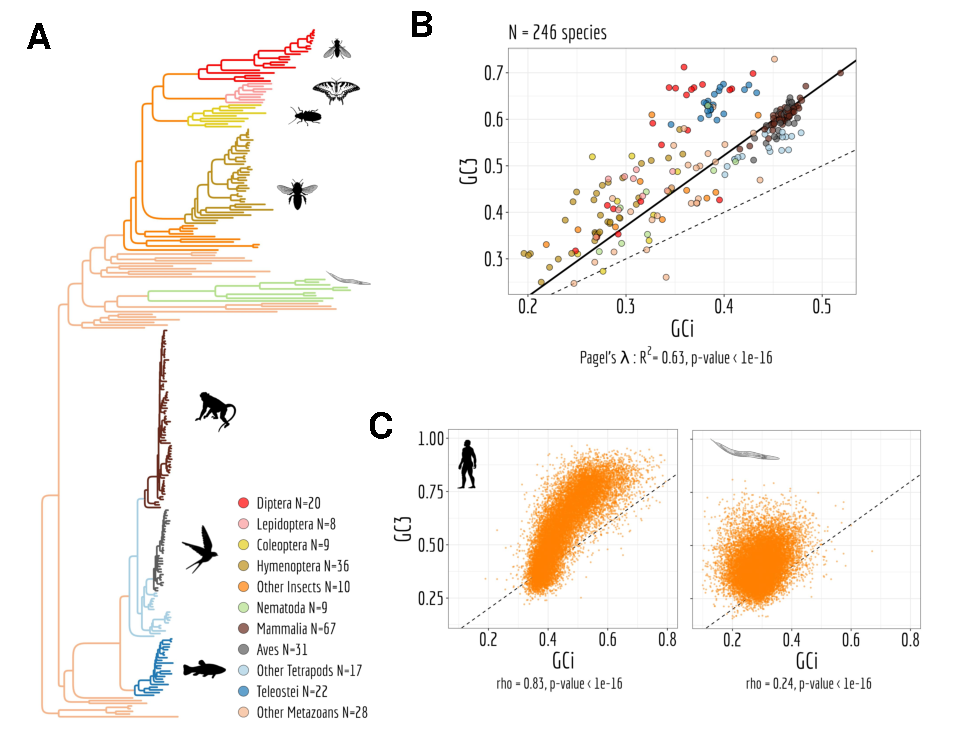
\includegraphics[width=\textwidth]{Figure1.pdf}
    \end{center}                                                                       
    \caption[Codon usage variations are driven by non-adaptive processes]{\textbf{Codon usage variations are driven by non-adaptive processes.} \textbf{A}: Phylogenetic tree of the 257 studied species. \textbf{B}: Gene average GC content at the third position of codons (GC3) and the gene average GC in introns (GCi) for each species. Pagel's \textit{lambda} model is used to take into account the phylogenetic structure of the data in a regression model (black line). \textbf{C}: Correlation between the gene GC3 and the GCi in \textit{Homo sapiens} (left) and in \textit{Caenorhabditis elegans} (right). Spearman's rho and corresponding p-values are displayed under the graph. The dotted lines correspond to x=y.}
    \label{fig:CU1}
\end{figure*}

NSPs can vary within the genome of a given species, and impact codon usage accordingly. In \textit{Homo sapiens}, the \textit{per} gene GC3 and GCi are highly correlated (Spearman's correlation coefficient, rho=0.83, p$<$$10^{-16}$), whereas this correlation is less pronounced in \textit{Caenorhabditis elegans} (rho=0.24, p$<$$10^{-16}$; \hyperref[fig:CU1]{Fig. 1C}). Species showing the strongest intra-genomic variance in codon usage (as assessed by  GC3) are the ones with the strongest variance in GCi \hyperref[suppfig:CU1]{Supplementary Fig. 1A}). These correlations between GC3 and GCi are particularly strong in tetrapods (107/108 species with rho$>$0.7) and in hymenopterans (25/35 species with rho$>$0.7)  (\hyperref[suppfig:CU1]{Supplementary Fig. 1B}). The other clades generally show less variance in GCi, and weaker correlations between GC3 and GCi. But overall, 244/246 species (99\%) showed a significant positive correlation (p$<$0.05), which indicates that in most species, intra-genomic variation in NSPs somehow contribute to the variance in SCU among genes. Hence, it is important to take this source of variance into account to be able to detect signatures of translational selection within genomes.

\subsection{tRNA abundance matches proteome requirements}

To quantify the intensity of translational selection, we used an approach similar to that of \citet{dos_reis_estimating_2009} and \citet{sharp_variation_2005}. This approach is based on the comparison of the frequency of optimal codons between highly and weakly expressed genes, and therefore requires the prior identification of optimal codons. For this, dos Reis and Wernisch focused on the nine amino-acids that are encoded by two codons (duet codons), and predicted the optimal codon of each amino-acid as being the one that is more frequently used in highly expressed genes. One caveat is that if the NSP varies among genes according to their expression level, this may lead to erroneous prediction of codon optimality. Furthermore, this approach does not capture the signal of translational selection from the nine other amino-acids that are encoded by triplet, quartet or sextet codons. To avoid these limitations, we sought here to predict optimal codons based on the tRNA pool. Owing to technical difficulties, there are currently few species for which tRNA abundance has been quantified directly. \citet{behrens_high-resolution_2021} recently developed a technique (mim-tRNAseq) that allowed them to measure tRNA abundance in four eukaryotes \citep{behrens_high-resolution_2021}. This study revealed a robust correlation between tRNA abundance and their respective gene copy number, with an adjusted $R^2 > 0.91$ for yeasts (\textit{S. cerevisiae} and \textit{S. pombe}), 0.79 for \textit{Drosophila melanogaster} and 0.62 for \textit{Homo sapiens}~\citep{behrens_high-resolution_2021}. These results suggest that tRNA copy numbers are a good predictor of tRNA abundances. To investigate whether the number of tRNA genes could be used as an indirect measure of tRNA abundance across metazoans, we analyzed the co-variation of their tRNA gene repertoires with the amino acid composition of their proteome.

The total number of tRNA gene copies varies widely among clades and species (ranging from an average of 201 tRNA gene copies per genome in hymenopterans to 1,537 copies in teleost fish; \hyperref[suppfig:CU2]{Supplementary Fig. 2}). However, the relative copy number of distinct isoacceptor tRNA genes is quite conserved among metazoans. There are some rare cases where the gene copy number of a given tRNA has exploded in a given species compared to other genomes (\hyperref[suppfig:CU2]{Supplementary Fig. 2}). This might reflect the propensity of tRNA genes to become transposable elements. Indeed many SINE retrotransposon families derive from tRNA genes \citep{sun_common_2007}, and it is therefore possible that some recently evolved SINEs are erroneously annotated as \textit{bona fide} tRNA genes.

In both \textit{Drosophila melanogaster} and \textit{Homo sapiens}, we observed a strong correlation between amino acid usage (\textit{i.e.} the frequency of amino acids, weighted by the expression level of genes) and direct measures of tRNA abundance (rho=0.79; \hyperref[suppfig:CU3]{Supplementary Fig. 3}; \citet{behrens_high-resolution_2021}). These results indicate that tRNA abundance matches the amino acid demand. As expected, the amino acid usage of these two species also strongly correlates with their tRNA gene copy numbers (rho=0.78 and 0.68 respectively; \hyperref[suppfig:CU3]{Supplementary Fig. 3}). As previously reported \citep{duret_trna_2000}, tRNA gene copy number also correlates with the amino acid demand in \textit{Caenorhabditis elegans} (rho=0.82; \hyperref[fig:CU2]{Fig. 2A}). The same analysis conducted across 246 animal species found a significantly positive Spearmann coefficient (\textit{i.e.} p-value $<$ 0.05) in 93\% of the species (\hyperref[fig:CU2]{Fig. 2B}), which indicates that in most of metazoans, the tRNA gene copy number is under constraints to match the amino acid demand. This implies that tRNA abundance is primarily regulated by modulating the copy number of tRNA genes rather than their transcription level. We suspect that the few cases where the number of tRNA genes does not correlate with amino acid usage might be due to annotation errors : some tRNA genes may have been missed (\textit{e.g.} because of gaps in the genome assembly), or conversely, some SINEs or tRNA pseudogenes may have been incorrectly annotated as functional tRNA genes. To ensure that the tRNA gene copy number is a good proxy of the tRNA abundance, we kept in our study only the species for which tRNA gene copy number correlates significantly with amino acid usage (N=230 species). We also excluded 7 species for which the repertoire of annotated tRNA appeared to be incomplete (\textit{i.e.} the cognate tRNAs of certain codons were not found in the genome assembly).

\begin{figure*}[t]
    \begin{center}
        \includegraphics[width=\textwidth]{Figure2.pdf}
    \end{center}                                                                       
    \caption[The tRNA gene copies number is a good predictor of the transcriptional requirements]{\textbf{The tRNA gene copies number is a good predictor of the transcriptional requirements.}
    \textbf{A}: The relationship between the number of tRNA gene copies \textit{per} amino acid and the frequency of amino acid weighted by gene expression (FPKM, log scale) in \textit{Caenorhabditis elegans}. Spearman's rho and corresponding p-value are displayed under the graph. \textbf{B}: Boxplot illustrating the distribution of Spearman's correlation coefficient ($\rho$) from Panel A for each species (N=246 species). The red line indicates the threshold above which the p-value is lower than 0.05.}
    \label{fig:CU2}
\end{figure*}


\subsection{Definition of putative-optimal codons based on tRNA abundance and wobble-pairing rules}

To predict which synonymous codons are optimal for translation, it is first necessary to associate each of the 61 codons to their cognate tRNA. The number of distinct isodecoder tRNAs (\textit{i.e.} distinct anticodons) ranges from 43 to 60 per species (average=47). This implies that 1 to 18 codons cannot be translated through Watson-Crick pairing (WCp), and hence have to be translated via wobble pairing (WBp). We used the rules established by Percudani \citep{percudani_restricted_2001} to assign each of these codons to their cognate tRNA, allowing for non-standard base pairing with the first nucleotide of the anticodon (\hyperref[fig:CU3]{Fig. 3A}). For example, deamination of adenine in inosine (I) in anticodons ANN makes them permissive to wobble pairing I:C; I:U or I:A. Another common wobble pairing is the G:U/U:G pairing~\citep{percudani_restricted_2001}. As an illustration, in human, asparagine is translated by a single tRNA (anticodon GTT) that decodes both AAC (by WCp) and AAT (by G:U WBp). AAT accounts for 48\% of asparagine codons, highlighting the significance of wobble pairing. 
There are 18 amino acids that are encoded by multiple synonymous codons. These amino acids can be classified in two groups:
- those whose synonymous codons are translated by at least two distinct isodecoder tRNAs 
- those for which all synonymous codons are translated by a single isodecoder tRNA 

There is some variation in the set of amino acids present in each group, depending on the isodecoder tRNA repertoire of each species. The first group generally corresponds to amino acids encoded by sextet codons (Leu, Arg, Ser), quartets (Val, Gly, Ala, Pro, Thr), triplet (Ile) and NNG/NNA duets (Glu, Gln, Lys). The second group corresponds essentially to the six amino acids encoded by NNC/NNT duets (Phe, Cys, Tyr, Asp, His, Asn) (\hyperref[fig:CU3]{Fig. 3B}).

For each amino acid of the first set, synonymous codons were predicted to be optimal if they were decoded by the isodecoder tRNA with highest gene copy number (\textit{i.e.} predicted to be the most abundant). In case of ex æquo (\textit{i.e.} if all synonymous codons are decoded by isodecoders having the same gene copy number), then the optimal codons of this amino acid were considered as unknown (76 ex æquo cases in total, in 62 species). In the cases where the most abundant tRNA decodes more than one synonymous codon, we considered all of them as potentially optimal (\textit{i.e.} at this stage, we do not make any assumption regarding which of the Watson-Crick pairing or wobble pairing is the most efficient). This first set of putative-optimal codons will hereafter be referred as 'POC1'.
The second set of amino acids corresponds to cases where the two synonymous codons (NNC/NNT) are decoded by a single isodecoder (anticodon GNN). There is evidence, based on studies in various eukaryotes, that the wobble pairing GNN:NNU is less efficient than the Watson-Crick pairing GNN:NNC~\citep{stadler_wobble_2011, chan_frequent_2017, wang_accurate_2017}. Consequently, for these amino acids, we defined codons NNC (decoded through WCp) as being the putative-optimal codons 'POC2'.

For the human genome, POC1 have been defined for 13 amino acids and POC2 for 5 amino acids. In contrast, for \textit{Caenorhabditis elegans}, POC1 and POC2 are defined for 12 and 6 amino acids, respectively. On average among the 223 species, POC1 are defined for 12.5 amino acids \textit{per} species (ranging from 8 to 17) and POC2 for 5.2 amino acids (ranging from 0 to 6, except \textit{Tyto alba} with 7 POC2, including Ile).

\begin{figure*}[t]   
    \begin{center}
        \includegraphics[width=\textwidth]{Figure3.pdf}
    \end{center}                                                                       
    \caption[Presence-Absence of tRNA defines set of putative-optimal codons]{\textbf{Presence-Absence of tRNA defines set of putative-optimal codons.} \textbf{A}: Illustration of the various possible pairings: Watson-Crick and wobble pairing. \textbf{B}: A boxplot illustrating the distribution of tRNA gene copy numbers across 223 species. The percentage of species lacking a tRNA gene copy is also indicated, highlighting the absence of tRNA isodecoder.}
    \label{fig:CU3}
\end{figure*}


\subsection{Highly expressed genes are enriched in optimal codons}

The intensity of translational selection depends directly on gene expression levels. Given the very wide range of variation of gene expression levels ($> 1000$ folds), the fitness impact of synonymous codon usage is expected to vary strongly among genes. Hence, a typical feature of genomes subject to translational selection (TS), is that the frequency of optimal codons is particularly high in the most highly expressed genes. Thus, to identify which species are subject to TS, we examined the variations in POC frequency according to gene expression level. To control for possible variations in neutral substitutions pattern, we also analyzed triplet content in introns, referred to as POC-control. It is important to note that the frequency of POC-control is not expected to be equivalent to that of the overall POC frequency due to the differing AT-richness of introns.

For \textit{Homo sapiens} POC frequencies show some slight fluctuations according to gene expression level (\hyperref[fig:CU4]{Fig. 4A}). However, the same weak fluctuations are observed for POC-controls in introns, which implies that a same process, independent of translation efficiency, affects the base composition, both in introns and at synonymous codon positions (\hyperref[fig:CU4]{Fig. 4A}). Indeed, there exists a strong correlation between the GC content of introns and the GC3 content in \textit{Homo sapiens}, along with pronounced variations in GC3 content (\hyperref[fig:CU1]{Fig. 1C}). In contrast, in \textit{Caenorhabditis elegans}, we observed a strong rise in POC frequencies in highly expressed genes, both for POC1 (from 47\% to 76\%) and for POC2 (from 38\% to 70\% ). These changes in codon usage are not caused by shift in local substitution patterns as we see no similar variation in POC-control (\hyperref[fig:CU4]{Fig. 4B}).


It is important to notice that the non-linear relationship observed between gene expression level and POC frequency is perfectly consistent with the TS model, that assumes that the selection coefficient on synonymous codon usage ($s$) should increase linearly with gene expression level. Indeed, this model predicts that for lowly expressed genes (such that $S = 4$\textit{N}$_{\text{e}}s \ll 1$), the frequency of optimal codons should evolve neutrally, and hence should be independent of expression level. But above the 'nearly-neutral' point (\textit{i.e.} the expression level for which $S\approx1$), the frequency of optimal codon should strongly increase with expression level (see \hyperref[appendices]{Appendices} for more details on equations). The shape of the POC1 and POC2 curves in \hyperref[fig:CU4]{Fig. 4B} indicates that in \textit{C. elegans}, this 'nearly-neutral' point is reached for a gene expression level of about 50 FPKM. This implies that genes with a lower expression level (which represent 83\% of genes in \textit{C. elegans}) are not affected by TS. Of note, the fraction of genes affected by TS is expected to be even more reduced in species with a lower effective population size.

To assess the impact of TS on synonymous codon usage, we measured the difference between the frequency of POCs in the most expressed genes (top 2\%), and the frequency of POCs in the 50\% lowest expressed genes, controlling for POCs-control variations (see \nameref{sec:MaterialsMethodsCU}). This shift in codon usage (denoted $\Delta POC^{exp}$ ) was computed for both POC1 and POC2 codons in each of the studied species (N=223 species). $\Delta POC_1^{exp}$ and $\Delta POC_2^{exp}$ are strongly correlated ($R^2=46$\% , p-value $< 10^{-16}$), which indicates that the signature of translational selection is effectively captured by both sets of codons (\hyperref[fig:CU4]{Fig. 4C}). For 211 species (95\%), the prevalence of POC1 is greater in highly expressed genes compared to other genes (\hyperref[fig:CU4]{Fig. 4D}). Similarly, $\Delta POC_2^{exp}$ is positive for 191 species (86\%; \hyperref[fig:CU4]{Fig. 4D}). The highest values of $\Delta POC^{exp}$ were observed in \textit{C. elegans} (+30\% for both POC1 and POC2). There are substantial variation across clades: average $\Delta POC_1^{exp}$ and $\Delta POC_2^{exp}$ values are around +14\% in Diptera compared to +3\% in vertebrates. We obtained very similar results when measuring $\Delta POC^{exp}$ without accounting for POC-control variations (\hyperref[suppfig:CU5]{Supplementary Fig. 5}). Given that the two sets of codons gave very consistent results, we hereafter considered the whole set of POCs regrouping both POC1 and POC2 .


\begin{figure*}[t]   
    \begin{center}
        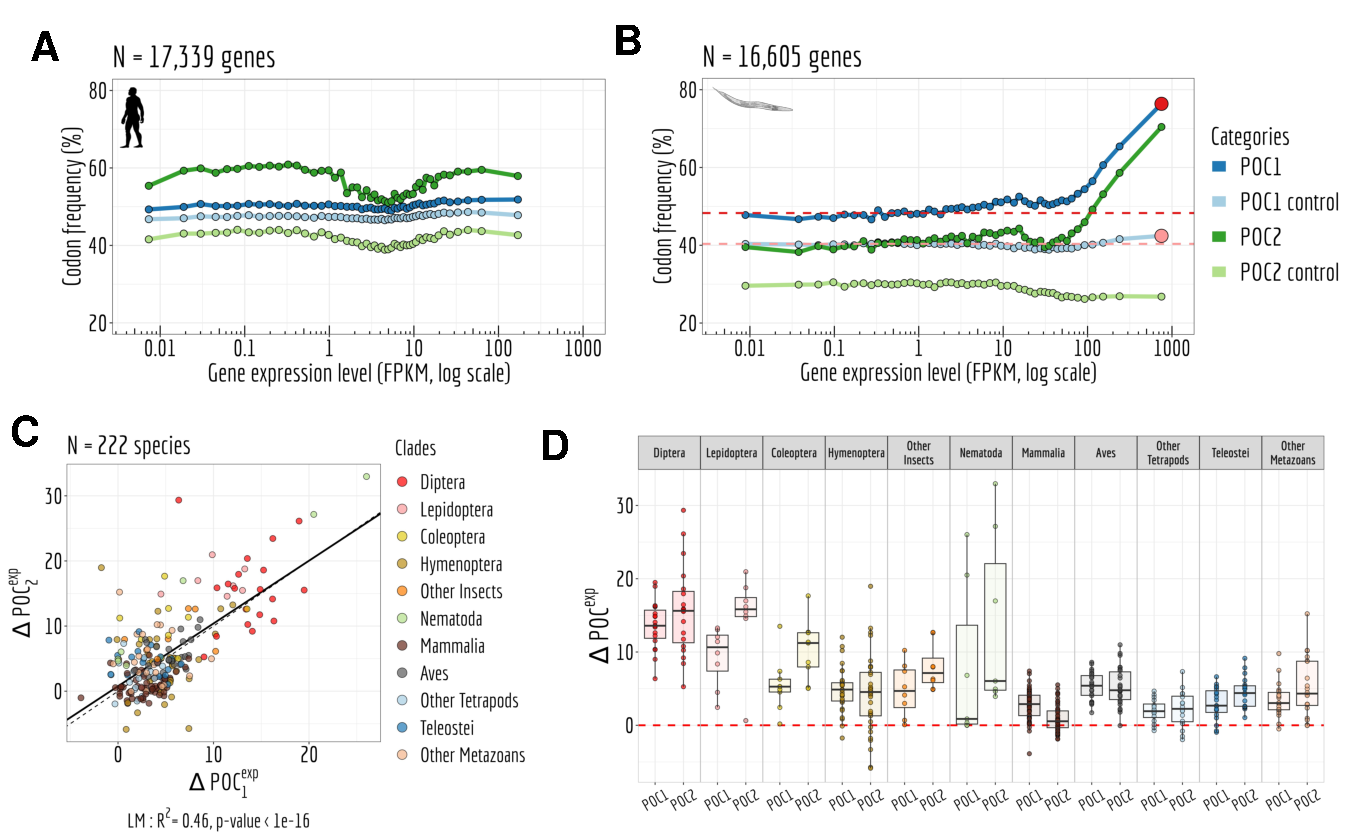
\includegraphics[width=\textwidth]{Figure4.pdf}
    \end{center}                                                                       
    \caption[Differences in usage of putative-optimal codon between highly- and lowly-expressed genes]{\textbf{Differences in usage of putative-optimal codon between highly- and lowly-expressed genes.} \textbf{A,B}: Variation in the proportion of POC within coding sequences (POC1: dark blue; POC2: dark green) according to gene expression level. To control for variations in neutral substitution patterns, we analyzed the frequency of corresponding triplets within introns (POC1 control: light blue; POC2 control: light green). Each point represents a 2\% bin of genes, with the red point at the end of each POC1 curve denoting the 2\% most highly expressed genes. The red lines indicate the average POC1 proportions observed in the 50\% least expressed genes (FPKM, log scale). \textbf{A} represents \textit{Homo sapiens} , and \textbf{B} represents \textit{Caenorabditis elegans}. \textbf{C}: Relation between the variations in POC1 and POC2 frequency with expression. Calculated as the difference between POC frequency in the 2\% most highly expressed genes and the 50\% least expressed genes. To this variations we removed variations measured on control. \textbf{D}: Boxplot illustrating the differences, for each species, between the TS intensity measured on POC1 and POC2.
    }
    \label{fig:CU4}
\end{figure*}


\subsection{Highly constrained amino acids are enriched in optimals codons}

Synonymous codon usage is expected to be under selection not only for its impact on the speed of translation, but also on the accuracy of translation. For both traits, selective constraints are expected to vary among genes, according to their expression level. One specific feature of selection for translation accuracy is that the strength of selection is also expected to vary among sites within a protein: selection on translation accuracy should be stronger at sites that are essential for the structure or function of the protein. 
To test this prediction, we analyzed within-gene variation in POC usage according to the level of constraint on amino acid sites. For this, we focused on a set of 976 orthologous genes, present in single copy in most metazoan genomes (BUSCO genes; \citet{waterhouse_busco_2018}). For each protein of a given species, we classified its sites into four groups of equal size, according to their level of conservation across 293 metazoans (see \nameref{sec:MaterialsMethodsCU}), and then measured the shift in POC frequency between its 25\% most conserved sites and its 25\% least conserved sites. Finally, we computed the average of these shift values over all proteins of this species (noted $\Delta POC^{cons}$). Given that the shift is computed within each gene, $\Delta POC^{cons}$ measures variation in codon usage across sites that inherently have the same expression level. 
One difficulty however is that in tetrapods, many genes contain a GC-rich CpG island at their 5' end \citep{deaton_cpg_2011}. The presence of a CpG island affects the base composition of the beginning of genes, up to about 1 kb, as illustrated by the analysis of the intronic GC content (\hyperref[suppfig:CU7]{Supplementary Fig. 7}). This results in differences in codon usage between the first exon and the rest of the coding region. Given that the N-termini of proteins evolve faster than their center \citep{bricout_evolution_2023}, this causes a spurious association between codon usage and variation in amino acid constraints along proteins. To avoid this bias, we measured $\Delta POC^{cons}$ in tetrapods only on codons located beyond 1 kb of the start codon (in genomic coordinates). In other clades, the base composition of introns shows little variation along genes (\hyperref[suppfig:CU7]{Supplementary Fig. 7}), and hence $\Delta POC^{cons}$ was measured on the entire coding region. 
In \textit{C. elegans}, the frequency of POC increased significantly between the least constrained and most constrained sites within proteins (from 48.5\% on average to average 51.2\%), whereas no variation was observed in humans (\hyperref[fig:CU5]{Fig. 5A,B}). Overall, $\Delta POC^{cons}$ is positive in 75\% of species (refer to \hyperref[fig:CU5]{Fig. 5C}). As for $\Delta POC^{exp}$ , $\Delta POC^{cons}$ shows substantial variation across clades, and is maximal for Diptera.



\begin{figure*}[t]   
    \begin{center}
        \includegraphics[width=0.75\textwidth]{Figure5.pdf}
    \end{center}                                                                       
    \caption[Most highly conserved regions exhibit a preference for using POCs]{\textbf{Most highly conserved regions exhibit a preference for using POCs.} \textbf{A,B}: Investigation of POCs frequency by dividing genes into four constraint groups of equal size, based on the gap proportion of gene alignments across all species. The frequency of POCs was calculated for each gene within each constraint group. A boxplot is shown, with darker green indicating the least constrained sites and darker red indicating the most constrained sites. \textbf{A} represents \textit{Homo sapiens}, and \textbf{B} represents \textit{Caenorabditis elegans}. \textbf{C}: Distributions depicting the average differences \textit{per} species between the frequency of POCs in highly constrained sites and unconstrained sites of given genes.}
    \label{fig:CU5}
\end{figure*}


\subsection{Selection favors optimal codons in highly expressed genes of \textit{Drosophila melanogaster}}

To further assess whether POCs are under selection in Diptera, we investigated patterns of polymorphism and substitution in \textit{Drosophila}, based on a multiple genome alignment of three closely related species (\textit{D. melanogaster, D. simulans, D. erecta}) and on single nucleotide polymorphism (SNP) data from 205 \textit{D. melanogaster} individuals. We inferred the ancestral and derived state at each substitution or SNP, so that to distinguish synonymous changes corresponding to POC to non-POC mutations (PO$>$nPO) vs non-POC to POC mutations (nPO$>$PO) (see \nameref{sec:MaterialsMethodsCU}; \hyperref[fig:CU6]{Fig. 6A}). To control for possible variation in local mutation patterns, we conducted a parallel analysis on triplets in intronic regions. In coding sequences (CDS), we identified 44,288 nPO$>$PO synonymous SNPs and 139,256 PO$>$nPO synonymous SNPs, 26,770 nPO$>$PO synonymous substitutions and 81,666 PO$>$nPO synonymous substitutions. In introns, we observed 187,321 nPO$>$PO SNPs and 260,366 PO$>$nPO SNPs, 56,916 nPO$>$PO substitutions and 77,686 PO$>$nPO substitutions. 

We observed that the rate of nPO$>$PO changes (number of nPO$>$PO changes/number of non-POC codons) increases with increasing gene expression level, while the rate of PO$>$nPO changes (number of PO$>$nPO changes/number of POC codons) decreased, both for SNPs and for substitutions(\hyperref[fig:CU6]{Fig. 6B,D}). Importantly, this trends is specific to coding regions, and is not observed for the corresponding triplets in introns (\hyperref[fig:CU6]{Fig. 6C,E}). These observations are consistent with the hypothesis that selection favors mutations leading to the incorporation of translationnally optimal codons in genes with high expression level.



\begin{figure*}[t]
    \begin{center}
        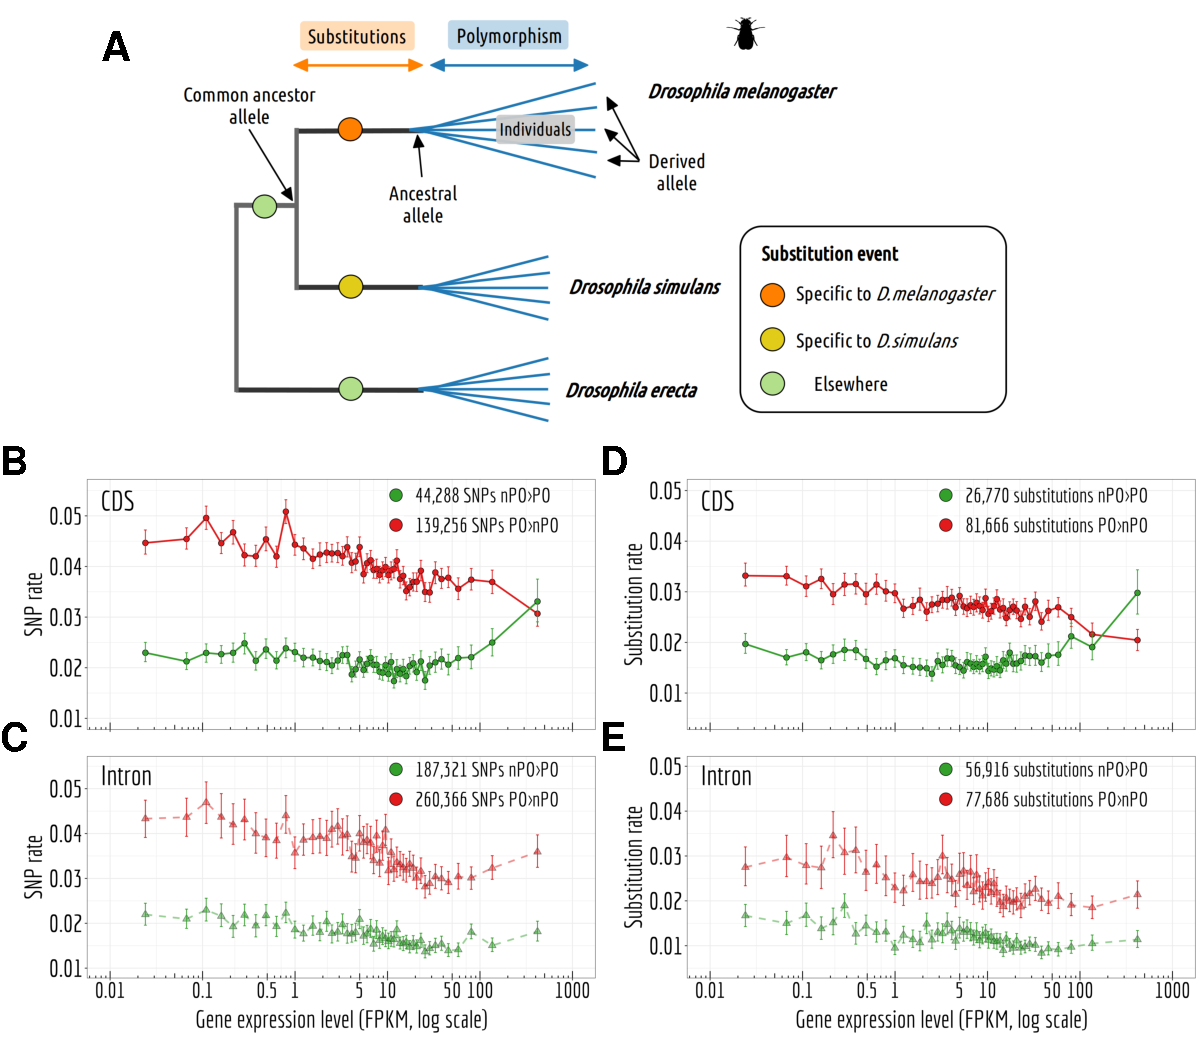
\includegraphics[width=0.9\textwidth]{Figure6.pdf}
    \end{center}                                                                       
    \caption[Selective pressure on non-POCs to POCs mutations]{\textbf{Selective pressure on non-POCs to POCs mutations.} \textbf{A}: Schematic representation of the method used to identify SNPs and substitutions in \textit{Drosophila melanogaster}. 
    \textbf{B,C}: Rate variations of SNPs non-POC towards POC (green) and POC towards non-POC (red) with gene expression in CDS (\textbf{B}) and in intronic control (\textbf{C}). 
    \textbf{D,E}: Rate variations of substitutions non-POC towards POC (green) and POC towards non-POC (red) with gene expression in CDS (\textbf{D}) and in intronic control (\textbf{E}). Error bars represent the 2.5th and 97.5th percentiles of values obtained from 100 simulations using a binomial distribution, following the same site structure and substitution rate (see \nameref{sec:MaterialsMethodsCU}).}
    \label{fig:CU6}
\end{figure*}

\subsection{Weak relationship between the strength of translational selection and the effective population size}

According to standard population genetic models of translational selection (\citet{bulmer_selection-mutation-drift_1991, sharp_variation_2005, dos_reis_estimating_2009}; \hyperref[appendices]{Appendices}), the difference in codon usage between highly and weakly expressed genes is expected to be directly linked to the population-scaled selection coefficient in favor of optimal synonymous codons ($S=4\textit{N}_{\text{e}}s$). Indeed, considering that synonymous codon usage evolves neutrally in lowly expressed genes, then $S$ in highly expressed genes can be expressed as: \begin{equation}S^{hx}=ln(\frac{FOP^{hx}}{1-FOP^{hx}})-ln(\frac{FOP^{lx}}{1-FOP^{lx}})\end{equation} where $FOP^{hx}$ and $FOP^{lx}$ are the observed frequencies of optimal codons in highly and lowly expressed genes respectively \citep{sharp_variation_2005, dos_reis_estimating_2009}. It should be noted however that this equation holds true only if underlying mutation patterns (and possibly gBGC) do not vary with gene expression level \citep{sharp_variation_2005, dos_reis_estimating_2009}. We used the above equation to estimate $S^{hx}$ in each species, based on the observed POC frequencies in the top 2\% most highly expressed genes, compared to the 50\% least expressed. The choice of this latter threshold is based on the observation that in species with clear signature of translational selection, POC frequencies show little variation in genes below the median expression level (\hyperref[fig:CU4]{Fig. 4B}; \hyperref[suppfig:CU9]{Supplementary Fig. 9}). 

If constraints on synonymous codon usage are similar across species (\textit{i.e.} if $s^{hx}$ is constant), then $S^{hx}$ is expected to vary linearly with the effective population size ($S^{hx}=4\textit{N}_{\text{e}}s^{hx}$). To test this prediction, we sought to estimate \textit{N}$_{\text{e}}$ for each species. Lynch and colleagues recently compiled a list of species for which the germline mutation rate ($\mu$) and the level of neutral diversity ($\pi_s$) have been measured, and hence for which it is possible to infer the effective population size ($N_{e}=\pi_{s}/4\mu$) \citep{lynch_divergence_2023}. This list included 24 species of our data set, and in addition allowed us to get a proxy of \textit{N}$_{\text{e}}$ for 17 species, for which species from the same genus were available. To explore the relationship between $S^{hx}$ and \textit{N}$_{\text{e}}$ in more species, we also used three indirect proxies (longevity, body length and the ${dN}/{dS}$ ratio) that correlate with the effective population size (\hyperref[suppfig:CU10]{Supplementary Fig. 10}). 

Among the 223 species analyzed, the strongest intensity of selection is observed in the nematodes \textit{C. elegans} ($S^{hx}=1.3$) and \textit{C. nigoni} ($S^{hx} =1.0$; \hyperref[fig:CU7]{Fig. 7}). Dipters also show relatively strong values of $S^{hx}$ (mean = 0.63±0.16 sd), followed by lepidopters (mean $S^{hx}$ = 0.41±0.15 sd). In vertebrates, signals of translational selection are weak (mean = 0.15±0.12 sd), but nevertheless, $S^{hx}$ are on average significantly non null (Student's t-Test, p-value $<10^{-16}$). Our estimates match with those previously published for \textit{C. elegans}, \textit{Drosophila melanogaster}, human and mice \citep{dos_reis_estimating_2009}. As predicted by the drift barrier model, the species with the strongest signs of translational selection all show a relatively short lifespan, low body mass and low dN/dS (\hyperref[fig:CU7]{Fig. 7B,D}), \textit{i.e.} traits associated to organisms with large \textit{N}$_{\text{e}}$. Conversely species with traits associated to low \textit{N}$_{\text{e}}$ all show low $S^{hx}$. However, the correlations between $S^{hx}$ and \textit{N}$_{\text{e}}$ proxies are weak, and significant for only two of them (longevity and dN/dS) (\hyperref[fig:CU7]{Fig. 7B,D}). The weakness of these correlation might be due to the fact that these traits are only indirect proxies of \textit{N}$_{\text{e}}$. However, even for the few species for which it is possible to get more direct estimates of \textit{N}$_{\text{e}}$ (based on $\pi_s$ and $\mu$), the correlation between $S^{hx}$ and \textit{N}$_{\text{e}}$ remains weak (\hyperref[fig:CU7]{Fig. 7A}). 

\begin{figure*}[t]   
    \begin{center}
        \includegraphics[width=\textwidth]{Figure7.pdf}
    \end{center}                                                                       
    \caption[Relationship between \textit{N}$_{\text{e}}$ and translational selection intensity ($S$)]{\textbf{Relationship between \textit{N}$_{\text{e}}$ and translational selection intensity ($S$).} 
    Relationship between the population-scaled selection coefficient (\textit{S}) and \textit{N}$_{\text{e}}$ (\textbf{A}), longevity (days, log scale; \textbf{B}), body length (cm, log scale; \textbf{C}), dN/dS (log scale; \textbf{D}). The translational selection intensity $S$ is measured on the top 2\% most highly expressed genes ($S^{hx}$). Pagel's \textit{lambda} model is used to take into account the phylogenetic structure of the data in a regression model (the regression line is displayed in black when the correlation is significant). Error bars represent the 2.5th and 97.5th percentiles of $S$ values obtained from 1000 draws with replacement among the top 2\% most highly expressed genes, and the 50\% least expressed.
    }
    \label{fig:CU7}
\end{figure*}


\subsection{In species subject to translational selection, the tRNA pool evolves in response to changes in neutral substitution patterns}

The above analyses show that for most metazoan species, translational selection is very weak, and hence that their synonymous codon usage is essentially shaped by neutral neutral substitution patterns (NSP). Interestingly, even in species with clear signal of translational selection, codon usage appears to be influenced by variations in NSP. Notably, Diptera and Lepidoptera span a wide range of GC-content in non-coding regions (genome-wide average GCi ranging from 0.25 to 0.43), that strongly correlates with their average GC3 (from 0.32 to 0.71; \hyperref[fig:CU1]{Fig. 1B}). Yet, most of Diptera and Lepidoptera show a strong translational selection compared to other metazoans (26 out of 27 species with $S^{hx}>$ 0.3, the only exception being \textit{Eumeta japonica}, with $S^{hx}$ = 0.09). This raises the question of how the tRNA pool evolved in these species in response to NSP changes. To investigate this point, we focused our analyses on the 26 Diptera and Lepidoptera species with a strong signal of translational selection.

In this dataset, we observed that the decoding of 11 NNA/NNG synonymous codon pairs (Glu, Gln, Lys, Val, Ala, Pro, Thr, Ser, both CTA/CTG and TTA/TTG pairs of Leu, and the AGA/AGG 'duet' of Arg) never involves wobble pairing: the two complementary isodecoder tRNAs (anticodons UNN and CNN, respectively) are systematically present altogether in their genome (\hyperref[suppfig:CU12]{Supplementary Fig. 12}). Thus, for each of these 11 pairs, we identified the 'preferred' isodecoder tRNA (\textit{i.e.} the one with the highest gene copy number) in each species. We observed that the proportion of the 11 preferred tRNAs having a CNN anticodon in a given species correlates positively with the GCi of species (\hyperref[fig:CU8]{Fig. 8A}). This implies that tRNA gene copy number co-evolved in response to changes in NSP, consistent with the hypothesis that tRNA abundance is under selective pressure to match the demand in synonymous codon usage. For the two other synonymous codon pairs CGG/CGA of Arg and GGG/GGA of Gly, the CNN-tRNA is absent in 67\% of cases, where UNN-tRNA decodes both codons NNA/NNG (\hyperref[suppfig:CU12]{Supplementary Fig. 12}). 

NNT/NNC synonymous codon pairs (N=16) are generally decoded by a single isodecoder tRNA (\hyperref[fig:CU3]{Fig. 3B}, \hyperref[suppfig:CU2]{Supplementary Fig. 2}). Among dipters and lepidopters, this is the case for 94\% of the 416 NNT/NNC synonymous codons pairs analyzed (16 pairs $\times$ 26 species; \hyperref[suppfig:CU12]{Supplementary Fig. 12}). In such cases, shifts in NSP cannot be compensated for by a change in the relative abundance of isodecoder tRNAs. Nevertheless, the affinity of tRNAs for their cognate codons can be changed by post-transcriptional modifications, and hence might evolve in response to the demand. To investigate whether such changes occur, it is necessary to identify which of the two codons is best decoded by this unique isodecoder tRNA. For this, we relied on the fact that in species that are subject to translational selection, codons that are more efficiently decoded show a higher prevalence in highly expressed genes compared to lowly expressed ones (these codons will hereafter be referred to as preferred codons). Two sets of NNT/NNC synonymous codons pairs can be distinguished: the 7 pairs corresponding to the amino acids with duet codons (Phe, Cys, Tyr, Asp, His, Asn and the AGT/AGC 'duet' of Ser), and the 9 pairs from amino acids with triplet (Ile) or quartet codons (Val, Gly, Ala, Pro, Thr, Leu, Arg, Ser). For NNT/NNC duets, when a single tRNA is present (95\% of cases), it is always the GNN-tRNA, and in 99\% of cases it is the NNC codon, decoded through Watson-Crick pairing that is preferred. For 8 of the 9 other pairs, when a single tRNA is present (94\% of cases), it is always the ANN-tRNA, the only exception being Gly (GNN-tRNA). For Gly, the GGT codon, decoded via wobble pairing, is preferred to the GGC codon in 84\% of species. For the other pairs (decoded by ANN-tRNA) there is more variability: the NNC codon (wobble pairing) is preferred in 79\% of species, whereas the NNT codon (watson-crick pairing) is preferred in the others. These observations indicate that when a single tRNA is present for two codons, it is not systematically the one with watson-crick pairing that is the most efficiently translated. Furthermore, although the NNC codon tends to be preferred to the NNT codon (except for Gly), there are some variation across species, notably for those decoded by a ANN-tRNA (\hyperref[suppfig:CU11]{Supplementary Fig. 11}). We computed in each species the proportion of NNC preferred codons among NNT/NNC synonymous codon pairs decoded by a single tRNA. Interestingly, the species showing the highest proportion of NNT preferred codons are the ones with the lowest genomic GC content (\hyperref[fig:CU8]{Fig. 8B}). Thus, it appears that the relative affinity of ANN-tRNAs for the NNT or NNC codon can evolve in response to the demand. 

These observations suggest a straightforward model to explain variation in the set of optimal synonymous codons across species (\hyperref[fig:CU8]{Fig. 8C}). First, variation in mutational patterns or in the intensity of gBGC can lead to changes in the base composition of genomes, thereby directly shifting the codon usage of genes. Given that translational selection is a weak force, most genes are affected by this shift. This results in a change in the codon demand, and hence induces a selective pressure to change the pool of tRNA (both in terms of abundance and of affinity for their cognate codons). In turn, translational selection will modify the codon usage of highly expressed genes to match the new set of tRNAs, thereby reinforcing the selection on the tRNA pool to match the codon demand, and resulting to a new co-adaptation between the tRNA pool and codon usage.


\begin{figure*}[t]   
    \begin{center}
        \includegraphics[width=0.9\textwidth]{Figure8.pdf}
    \end{center}                                                                       
    \caption[Genomic substitution pattern shapes the tRNA pool]{\textbf{Genomic substitution pattern shapes the tRNA pool.} \textbf{A}: Relashionship between the \textit{per} species CNN fraction of preferred isodecoder tRNAs (corresponding to the most abundant tRNAs) among 11 NNA/NNG synonymous codon pairs and the gene average GC in introns (GCi), for Diptera (dark red) and Lepidoptera (light red). \textbf{B}: Relashionship between the \textit{per} species proportion of NNC preferred codons (the most overused codons in highly expressed genes compare to lowly expressed genes) among NNT/NNC synonymous codon pairs decoded by a single tRNA, along with the GCi. \textbf{A,B}: Pagel's \textit{lambda} model is used to take into account the phylogenetic structure of the data in a regression model (black line if significant). \textbf{C}: Hypothetical schemes explaining how synonymous codon usage can be shaped conjointly by translational selection and by neutral substitution patterns.}
    \label{fig:CU8}
\end{figure*}


\subsection{Weak translational selection in species with large intra-genomic variability in neutral substitution patterns}

An implicit assumption of the above model is that all genes of a given genome are affected by similar neutral substitution patterns. There is evidence however that some genomes are subject to heterogenous neutral substitution patterns. Notably, in mammals and birds, variation in recombination rates along chromosomes induce a strong heterogeneity in GC-content, driven by gBGC ~\citep{duret_biased_2009}. This process accounts for 70\% of the variance in synonymous codon usage among human genes \citep{pouyet_recombination_2017}. Thus, in these species, the synonymous codon usage of a given gene essentially depends on the base composition of the genomic region where it resides, as shown by the strong correlation observed between GC3 and GCi across human genes (\hyperref[fig:CU1]{Fig. 1C}). It is important to notice that these regional variations in GC-content affect all genes, even those that are widely expressed. To illustrate this point, we analyzed the codon usage of 2,249 human housekeeping genes (defined as genes that are in the top 20\% most highly expressed genes in at least 75\% of tissues). The distribution of GC3 in housekeeping genes shows a very strong heterogeneity (GC3 ranging from 25\% to 95\%; \hyperref[fig:CU9]{Fig. 9B}), as strong as in the entire gene set (\hyperref[fig:CU9]{Fig. 9A}). Housekeeping genes are involved in basal function and have to be expressed at high level in most cell types. This implies that in any given cell, there is a strong heterogeneity of the codon demand. Such a situation is predicted to hinder the co-adaptation between the tRNA pool and codon usage: any increase in the abundance of a given tRNA (say decoding a GC-ending codon) is expected to be beneficial for the translation of GC-rich genes, but detrimental for the translation of the GC-poor ones (and vice versa for a tRNA decoding an AU-ending codon). Hence, the selective pressure imposed by the codon demand is expected to maintain a balanced tRNA pool, able to decode GC-rich genes as well as GC-poor genes. In turn, the presence of a balanced tRNA pool should reduce the difference in translational efficiency between synonymous codons, and hence is expected to decrease the intensity of translational selection. Thus, genomes that are subject to heterogenous neutral substitution patterns are expected to be less subject to translational selection.
To test this prediction, we analyzed the relationship between the intensity of translational selection ($S^{hx}$) and the intra-genomic heterogeneity in base composition (assessed by the variance in GCi across genes). We observed that all species with a strong signal of translational selection show a very small variance in GCi, while species with a high variance in GCi show relatively low $S^{hx}$ (\hyperref[fig:CU9]{Fig. 9C}). This is consistent with the hypothesis that intra-genomic heterogeneity in base composition precludes translational selection. However, species with a high variance in GCi mainly correspond to three clades (Mammal, Aves, Hymenoptera) that have relatively small \textit{N}$_{\text{e}}$, and hence it is difficult to disentangle the impact of intra-genomic heterogeneity in base composition from that of drift (\hyperref[fig:CU9]{Fig. 9D}). 
In any case, even though intra-genomic heterogeneity in base composition might explain the weakness of translational selection in some species, there must be some other factors that affect the intensity of translational selection. Indeed, among insect species predicted to have a \textit{N}$_{\text{e}}$ similar to that of dipters, many show a low $S^{hx}$ despite a small variance in GCi (\hyperref[fig:CU9]{Fig. 9E,F}). 


\begin{figure*}[t]   
    \begin{center}
        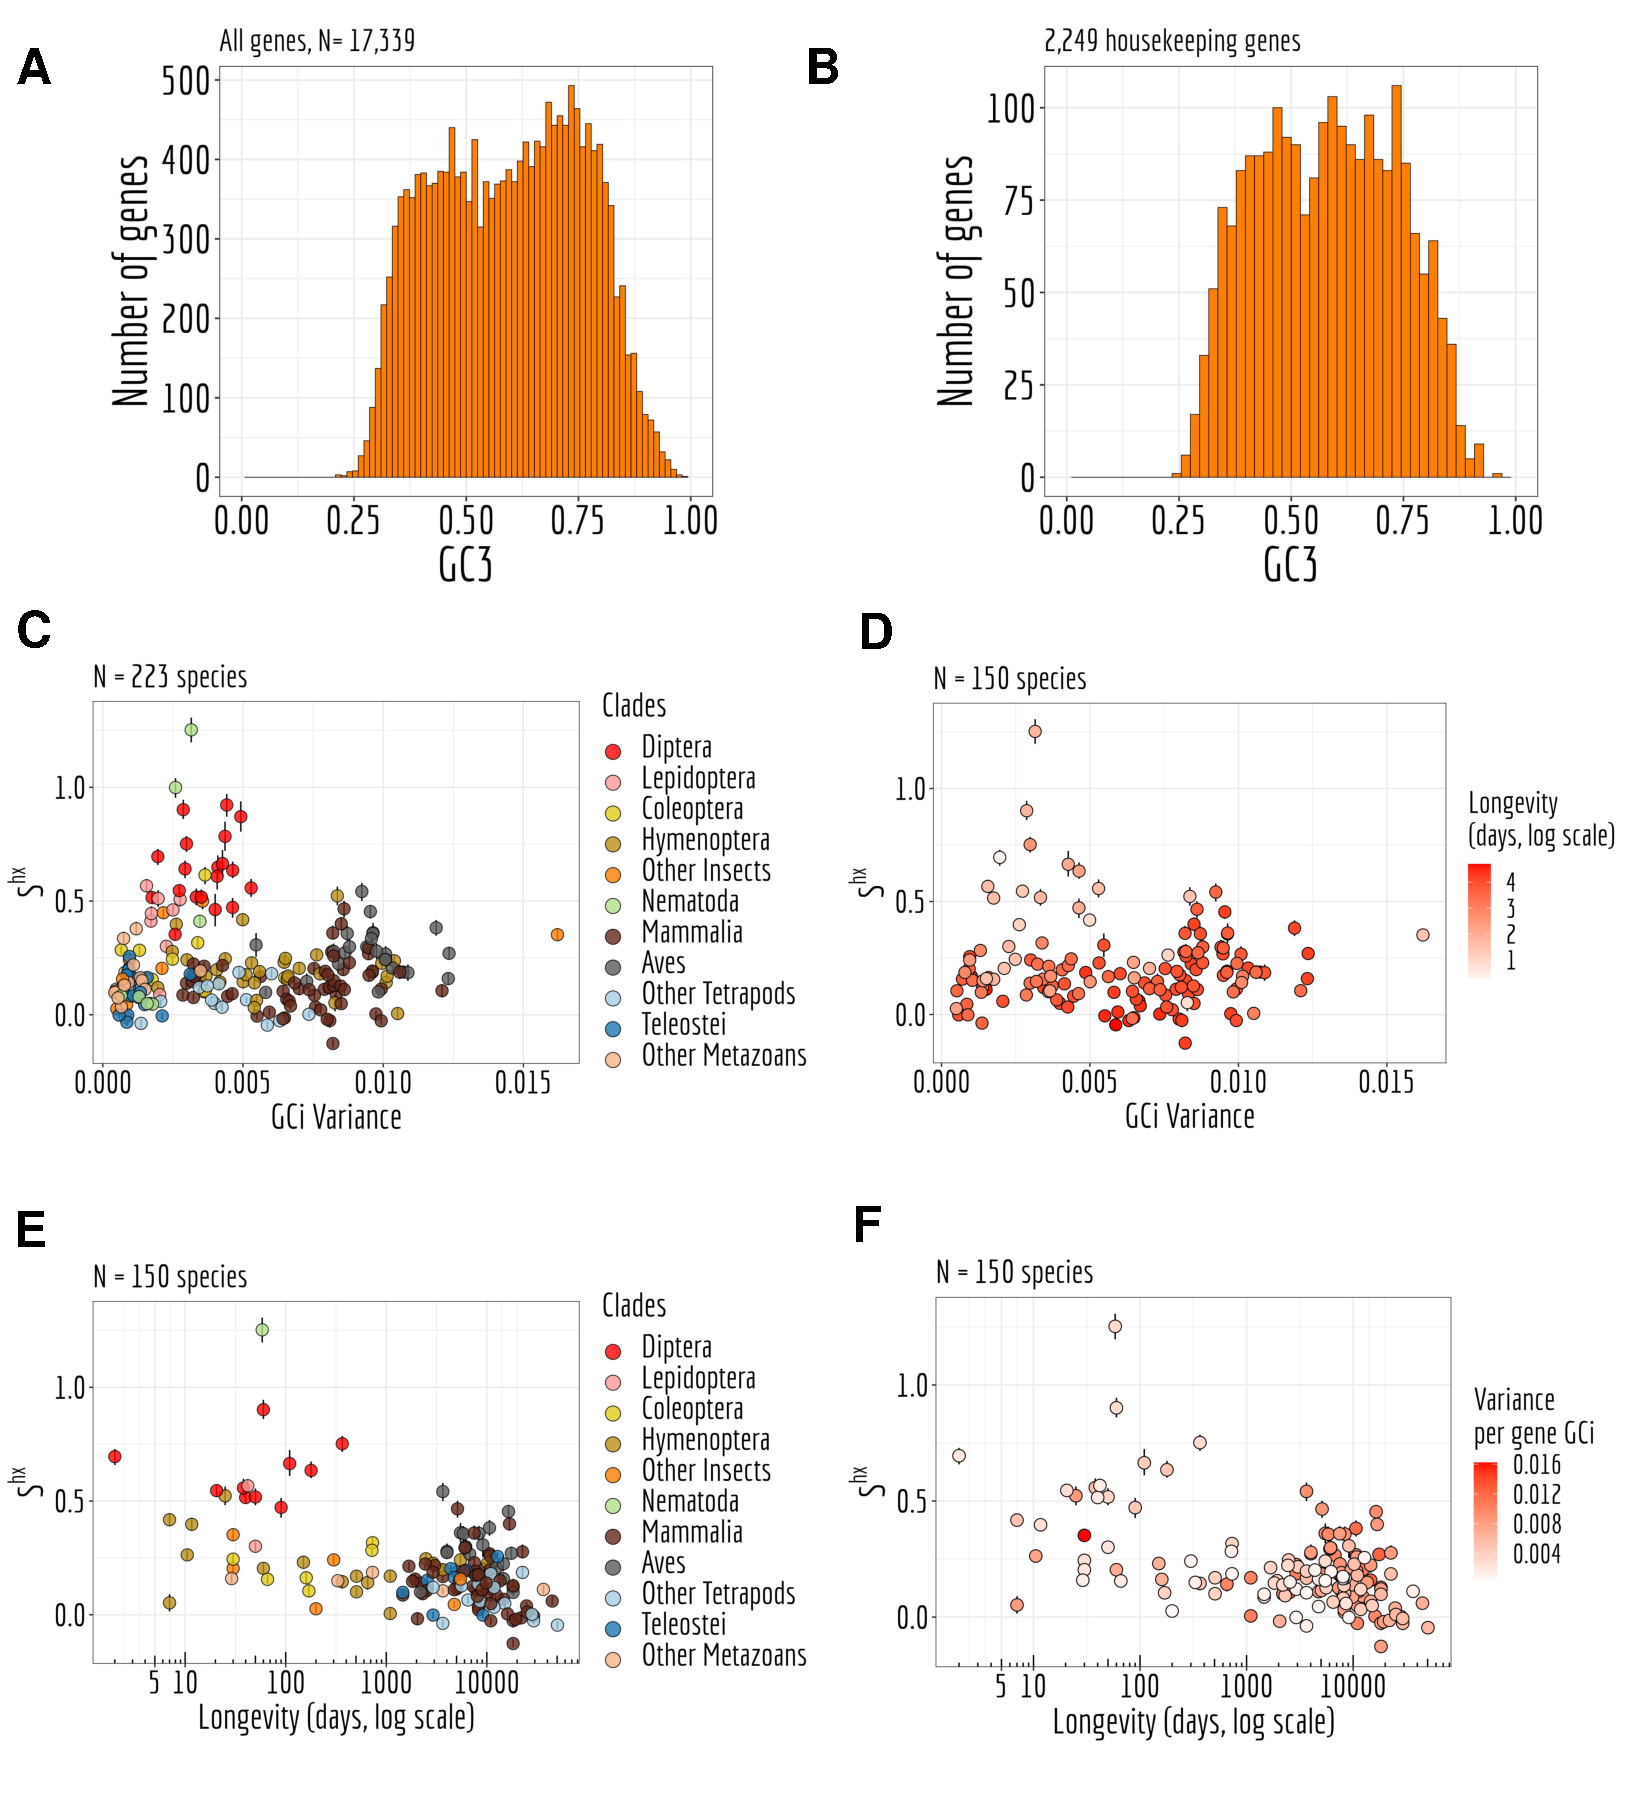
\includegraphics[width=0.7\textwidth]{Figure9.pdf}
    \end{center}                                                                       
    \caption[Large intra-genomic variability in neutral substitution patterns impact on translational selection]{\textbf{Large intra-genomic variability in neutral substitution patterns impact on translational selection.} \textbf{A}: Distribution of GC content at the third position of codons (GC3) across human genes. \textbf{B}: Distribution of GC3 across human housekeeping genes (identified based on gene expression data from 27 healthy tissues, extracted from~\citep{pouyet_recombination_2017}. \textbf{C,D}: Relation between translational selection intensity \textit{S} and the gene GCi variance. \textbf{D}: Species are colored with a longevity gradient (log scale). \textbf{E,F}: Relation between translational selection intensity \textit{S} and longevity (days, log scale). \textbf{F}: Species are colored with a GC intron variance gradient (log scale).}
    \label{fig:CU9}
\end{figure*}




\section{Discussion}

\subsection{Predicting translationally optimal codons}

Patterns of SCU vary widely across metazoan species, and are strongly correlated to the base composition of their non-coding regions (\hyperref[fig:CU1]{Fig. 1A}). This implies that variation in codon usage across species are primarily shaped by differences in genome-wide neutral substitution patterns (driven by the underlying mutation pattern, by gBGC or both). NSPs vary not only across species, but also along chromosomes, and in some clades, such as tetrapods or hymenopters, this intra-genomic heterogeneity of NSPs is a major determinant of the variance in SCU among genes (\hyperref[suppfig:CU1]{Supplementary Fig. 1B}). The fact that genome-wide patterns of SCU are strongly affected by NSPs does not exclude that it can also be shaped by a selective pressure favoring the use of translationally optimal codons. Indeed, in dipters and lepidopters, which both show clear evidence of translational selection, we observed that the tRNA pool evolves in response to changes in genome-wide NSPs (\hyperref[fig:CU8]{Fig. 8}). Thus, variation in NSPs can lead to shifts in the translation apparatus, and thereby drive the evolution of SCU, not only in weakly expressed genes where codon usage is effectively neutral, but also in genes under strong translational selection. In other words, selective and non-adaptive models are not mutually exclusive, but it is important to take NSPs into account to be able to detect signatures of translational selection within genomes.

To quantify the intensity of translational selection in metazoans, we used a method based on standard population genetics equations, that infers the population-scaled selection coefficient ($S=4\textit{N}_{\text{e}}s$) from the difference in optimal codon frequency between highly expressed genes and weakly expressed genes \citep{sharp_variation_2005, dos_reis_estimating_2009}. This method first requires to identify the set of optimal codons in each species. To predict optimal codons, previous studies generally searched for codons whose frequency increases with gene expression level (\textit{e.g.} \citet{duret_expression_1999, dos_reis_estimating_2009}). One caveat, is that in some species, NSP varies with gene expression \citep{pouyet_recombination_2017}, which may therefore lead to errors in the inference of optimal codons. Furthermore, in that situation, the method would systematically overestimate $S$ for codons that are favored by NSPs in highly expressed genes. To limit this bias, we sought to predict optimal codons from the tRNA pool available in each species. For this, we estimated the abundance of each tRNA based on its gene copy number in the genome. In most species, we observed a strong correlation between the number of iso-acceptor tRNA gene copies and the frequency of their cognate amino-acid in the proteome (\hyperref[fig:CU3]{Fig. 3B}). These strong correlations are consistent with the fact that cellular tRNA abundance is highly constrained to match the amino-acid demand, and indicate that tRNA gene copy number is a good proxy to infer tRNA abundance, in agreement with previous experimental evidence from a limited set of species \citep{behrens_high-resolution_2021}.
Based on our estimates of the tRNA pool, we predicted two sets of putative optimal codons (POCs): for amino acids for which more than one iso-decoder tRNA is available, optimal synonymous codons were defined as those decoded by the most abundant tRNA (POC1); for amino acids encoded by NNC/NNU duet codons and with one single iso-decoder tRNA (GNN), the NNC codons were predicted to be optimal (POC2), based on previous studies showing that the wobble pairing GNN:NNU was less efficient than the Watson-Crick pairing GNN:NNC (\citet{stadler_wobble_2011, chan_frequent_2017}; \hyperref[fig:CU3]{Fig. 3B}).

Several lines of evidence indicate that our predictions of translationally optimal codons are accurate. First, our sets of POCs are consistent with previous predictions: we identified 25 POCs in \textit{C. elegans} and 27 in \textit{D. melanogaster}, while respectively 26 and 25 optimal codons had been inferred based on difference in codon usage between highly and lowly expressed genes \citep{duret_expression_1999}, of which 88.4\% and 88.0\% match with our POCs. Furthermore, the analysis of substitution patterns and polymorphism in \textit{Drosophila melanogaster} confirmed that selection favors POC alleles over non-POC alleles in highly expressed genes (\hyperref[fig:CU6]{Fig. 6}). Finally, we observed that although the definition of POC1 and POC2 relies on very different principles, the two sets of codons show very similar signatures of translational selection (\hyperref[fig:CU4]{Fig. 4C}). 

\subsection{Variation in the intensity of selection in favor of translationally optimal codons across metazoans}

For each species, we measured the frequency of optimal codons (combining POC1 and POC2) in highly expressed genes (top 2\%), to estimate the population-scaled selection coefficient in favor of translationally optimal codons ($S=4\textit{N}_{\text{e}}s$), using weakly expressed genes as a reference to account for the NSP \citep{sharp_variation_2005}. Across the 223 species, the highest values of $S$ are observed in Caenorhabditis nematodes ($S=1.25$ in \textit{C. elegans} and $S=1.00$ in \textit{C. nigoni}). We also found a clear signal of translational selection in diptera (mean $S=0.63$, N=19 species), and to a lesser extent in lepidoptera (mean $S=0.41$, N=8 species). Overall, estimates of $S$ are weaker in other clades (\hyperref[fig:CU7]{Fig. 7}). The weakness of translational selection in vertebrates (mean $S=0.16$, N=100 species) was a priori expected given that these organisms tend to have relatively small \textit{N}$_{\text{e}}$. But besides Caenorhabditis and dipters, our dataset included 83 invertebrate species covering a wide range of clades (58 other insects, 12 other Ecdysozoa, 6 Spiralia, 4 Cnidaria, 3 Deuterostomia). What is surprising is that all these species show $S$ values that are lower than the average of dipters. This implies that the high values of $S$ observed in Caenorhabditis and in dipters represent exceptions rather than the rule, and that translational selection is weak in most metazoan lineages.

If the selection coefficient in favor of optimal codons ($s$) was constant across metazoans, then S should scale linearly with \textit{N}$_{\text{e}}$. To test this prediction, we used silent-site polymorphism and germline mutation rate data \citep{lynch_divergence_2023} to estimate the effective population size ($N_{e}=\pi_{s}/4\mu$, hereafter noted \textit{N}$_{\text{e}}^{\pi\mu}$) in 41 species. As expected $S$ tends to increase with \textit{N}$_{\text{e}}^{\pi\mu}$, but the correlation is not significant after accounting for phylogenetic inertia (\hyperref[fig:CU7]{Fig. 7A}). The weakness of the correlation might be due to the fact that these two parameters evolve on different time scales: \textit{N}$_{\text{e}}^{\pi\mu}$ is indicative of the recent effective population size (on the order of \textit{N}$_{\text{e}}$ generations) and hence can change quite rapidly compared to $S$, that is estimated from the codon composition of genomes, resulting from a long-term accumulation of substitutions. This can explain why \textit{C. nigoni} and \textit{C. elegans} display similar values of $S$, despite a 75-fold difference in \textit{N}$_{\text{e}}^{\pi\mu}$ (respectively \textit{N}$_{\text{e}}^{\pi\mu} =9.4\times 10^{6}$ and \textit{N}$_{\text{e}}^{\pi\mu}=1.2\times 10^{5}$). This difference in \textit{N}$_{\text{e}}^{\pi\mu}$ is due to the fact that \textit{C. nigoni} is an outcrossing species, like most other Caenorhabditis species, while the \textit{C. elegans} lineage evolved towards selfing hermaphroditism \citep{li_specialist_2014, vielle_convergent_2016}. This transition in reproductive mode is recent, and hence the SCU of \textit{C. elegans} still retains the signature of strong translational selection inherited from its outcrossing ancestors. Thus, we can predict that the SCU of \textit{C. elegans} is not at selection-mutation-drift equilibrium (which could be tested by analyzing synonymous polymorphism). 

To further test the relationship between $S$ and \textit{N}$_{\text{e}}$, we considered three parameters (longevity, body length and dN/dS), that are all correlated with \textit{N}$_{\text{e}}^{\pi\mu}$ (\hyperref[suppfig:CU10]{Supplementary Fig. 10}), but that are expected to reflect \textit{N}$_{\text{e}}$ over a longer time scale. A further interest of these proxies is that they can be estimated on much larger datasets (150 to 223 species). But here again we obtained similar results: $S$ tends to increase with \textit{N}$_{\text{e}}$, but correlations are weak, marginally significant after accounting for phylogeny (\hyperref[fig:CU7]{Fig. 7B,C and D}). The weakness of the correlation is mainly due to the fact that some species have a low $S$, despite life-history traits or dN/dS values indicative of a high \textit{N}$_{\text{e}}$.

Not only the correlations between \textit{N}$_{\text{e}}$ and $S$ are weak, but also the range of variation in $S$ appears to be quite limited compared to what would be expected given the variance in \textit{N}$_{\text{e}}$.
For instance, the mean value of \textit{N}$_{\text{e}}^{\pi\mu}$ is about 15 times higher in diptera than in mammalia (based on respectively 6 and 41 species for which \textit{N}$_{\text{e}}^{\pi\mu}$ can be estimated; \citet{lynch_divergence_2023}). Yet, the mean value of $S$ is only 5.3 times higher in diptera (mean $S=0.63$, N=19 species) than in mammals (mean $S=0.12$, N=65 species). Thus, the difference in $S$ between diptera and mammals is smaller than what would be expected if $S$ scaled linearly with \textit{N}$_{\text{e}}$.

One possible explanation for this discrepancy is that $S$ is overestimated in mammals. As discussed by \citet{dos_reis_estimating_2009}, the estimate of $S$ is based on the assumption that NSPs are constant across genes, \textit{i.e.} that the difference in optimal codon frequency between highly and weakly expressed genes is entirely due to translational selection. In reality, in some species, NSPs vary with gene expression (\textit{e.g.} in humans \citet{pouyet_recombination_2017}). To try to account for these variations, we measured the differences in POC frequency between highly and weakly expressed genes, controlling for differences in the corresponding triplet frequencies in introns. It is however possible that the base composition of introns is not a perfect predictor of NSPs, notably because introns are affected by indels and transposable elements, which are not allowed in coding regions. This is well illustrated by POC2 codons in humans, whose frequency clearly covaries with their non-coding controls, but with a wider amplitude in exons than in introns (\hyperref[fig:CU4]{Fig. 4A}).

An alternative hypothesis is that the discrepancy might result from a strong heterogeneity in the fitness effect of synonymous mutations. Indeed, the analysis of synonymous polymorphism in \textit{D. melanogaster} indicated that a majority of codons are under weak selection in favor of translationally optimal codon ($|$\textit{N}$_{\text{e}} s|\approx1$), but that a small fraction (10\%-20\%) are under strong selection ($|$\textit{N}$_{\text{e}} s|>10$; \citet{machado_pervasive_2020}. With a \textit{N}$_{\text{e}}$ value 15 times lower, the first class of codons is expected to evolve neutrally in mammals. But the second class of codons would still appear under effective translational selection, which might explain the small but non-null value of $S$ measured in mammals.

One last unexpected observation is that many species predicted to have a high \textit{N}$_{\text{e}}$ (based on their LHTs or dN/dS) show very weak $S$ (\hyperref[fig:CU7]{Fig. 7B,C and D}). In some species, this could be explained by the heterogeneity of NSPs along chromosomes, inducing a strong variance in SCU that precludes a co-adaptation of the tRNA pool. This might be the case notably for some hymenopters, which, like tetrapods, are subject to gBGC \citep{wallberg_extreme_2015} and present a very strong heterogeneity in NSPs (\hyperref[fig:CU9]{Fig. 9C}). However, our dataset also includes some species with small $S$ values, despite a high \textit{N}$_{\text{e}}$ proxy and homogenous NSPs. So finally, we are left with the conclusion that variation in $S$ across metazoans are not driven simply by the drift barrier and by gBGC, but that they are also probably due to variation in s, the selection coefficient in favor of translationally optimal codons. There is evidence that in unicellular organisms, the selective force for the optimization of SCU is the maximization of cellular growth \citep{rocha_codon_2004, sharp_variation_2005}. It is possible that the selective pressure on cellular growth also vary across metazoans. Most Caenorhabditis species grow in ephemeral environments (rotting vegetation) and hence have been selected for their capacity to proliferate very rapidly \citep{cutter_caenorhabditis_2015}. \citet{manthey_rapid_2024} recently quantified growth rates in 33 insects. The only dipter present in their dataset (\textit{Lucilia sericata}) is the species that presented the highest growth rate, 12 times higher than the average growth rate of other holometabole insects (N=10) and 52 times higher than the average growth rate of hemimetabole insects (N=22). If the \textit{Lucilia sericata} is representative of other dipters, this might explain why translational selection is particularly strong in that clade compared to other insects. It is noteworthy that the two invertebrate species that have been historically used as model organisms (\textit{D. melanogaster} and \textit{C. elegans}) both belong to the very rare metazoan clades with clear evidence of translational selection. This might reflect the fact that they have been chosen a model organisms for the very reason that they can grow very fast in the lab.





\section{Materials \& Methods}
\label{sec:MaterialsMethodsCU}


\subsection{Gene expression and data collection}

The reference genome assemblies and genome annotations were acquired from the National Center for Biotechnology Information (NCBI; \citet{sayers_database_2022}.
We obtained gene expression data for 257 metazoan species from GTDrift~\citep{benitiere_gtdrift_2024}, where Fragment \textit{Per} Kilobase of exon \textit{per} Million mapped reads (FPKM) was estimated over thousands of RNA-seq samples using cufflinks. For each species we considered the \textit{per}-gene median FPKM values across all analyzed RNA-seq samples.
Additionally, a phylogenetic tree was retrieved from GTDrift to account for phylogenetic inertia \citep{benitiere_gtdrift_2024}.


\subsection{tRNAscan-SE annotation}

If for a given species tRNA genes copies were previously annotated and so present in the NCBI annotation file, we took these annotations into account (N=44 species). Other wise (N=213 species) we annotated tRNA gene copies using the program tRNAscan-SE 2.0.12 (Nov 2022), with the -E option specifically designed for eukaryotic tRNA identification search~\citep{chan_trnascan-se_2021}. To keep in the study functional gene copies we retained those with a score exceeding 55, threshold based on~\citet{chan_trnascan-se_2021} analysis. Thus, for each of these copies we obtained the decoded codon and the translated amino acid. 

% command: tRNAscan-SE -E -o tRNA.tab -S off file-out

\subsection{Codon usage}

For each species in our study, we conducted a detailed assessment of codon usage across the longest annotated coding sequences (CDS) of each expressed gene within our dataset. This analysis was paralleled by an examination of the occurrences of nucleotide triplets within intron regions. It is important to note that our analysis deliberately excluded the acceptor and donor splice sites to avoid skewing the results with these highly conserved motifs.


\subsection{Site constraint}

Multiple gene alignments of 976 BUSCO genes and 293 species were collected to study site constraints from the metazoa dataset alignment of GTDrift repository~\citep{benitiere_gtdrift_2024}. For each gene, we determined the proportion of gaps at each site across the alignment. This information guided the \textit{per}-species segmentation of genes into bins, with each bin representing 25\% of a gene sequence. Our examination of tetrapods focused on sites located beyond 1,000 base pairs downstream from the start codon.


\subsection{SNPs analysis}

We used polymorphism data from the \textit{Drosophila} Genetic Reference Panel 2 (DGRP2)~\citep{mackay_drosophila_2012, huang_natural_2014}, where polymorphic sites have been identified from comparisons across 205 inbred lines of \textit{Drosophila melanogaster}, downloaded from \url{http://dgrp2.gnets.ncsu.edu/data/website/dgrp2.vcf}. We converted the single nucleotide polymorphism (SNP) coordinates from the dm3 genome assembly to the dm6 assembly, with the liftOver utility~\citep{hinrichs_ucsc_2006} of the UCSC genome browser, using a whole genome alignment between the two assemblies downloaded from \url{https://hgdownload.soe.ucsc.edu/goldenPath/dm3/liftOver/dm3ToDm6.over.chain.gz}. We kept in the study 3,738,302 biallelic SNPs for which more than 181 individuals have been genotyped.

We then identified two sister species \textit{Drosophila simulans} and \textit{Drosophila erecta} that we aligned against \textit{Drosophila melanogaster} genome using liftOver utility \citep{hinrichs_ucsc_2006}. We removed from the analysis genes located in regions where the multiple alignment was of poor quality (\hyperref[fig:CU8]{Supplementary Fig. 8}. We used the program est-sfs release 2.04~\citep{keightley_inferring_2018} to polarize SNPs, \textit{i.e.} to identify the ancestral allele and the derived allele. 

For the longest annotated coding sequence of each expressed gene we were able to identify the ancestral and derived codons for each SNP. The same approach was applied for intron regions by studying nucleotide triplets.

To determine the confidence interval for each data point (\hyperref[fig:CU6]{Fig. 6}), we employed a simulation approach. We simulated a sample with a similar structure in terms of the number of sites \textit{per} gene and the SNP rate, using a binomial distribution. We calculated the average SNP rate for each simulation, repeating the process 100 times. Afterward, we utilized the 2.5th and 97.5th percentiles of these mean values to establish the error bars.

\subsection{Substitutions analysis}

Based on the multiple genome alignment of \textit{Drosophila simulans}, \textit{Drosophila erecta} and \textit{Drosophila melanogaster} previously described, we identified the non polymorphic sites where a substitution occurred. To do so, we studied sites for which we were able to determine the ancestral and substituted allele by considering the most parsimonious scenario :
if reference alleles of \textit{D.erecta} = \textit{D.melanogaster} or \textit{D.simulans} = \textit{D.melanogaster} there is no substitution;
if reference alleles of \textit{D.erecta} = \textit{D.simulans} but differ from \textit{D.melanogaster} then there is a substitution and the ancestral allele is the one observed on \textit{D.erecta} and \textit{D.simulans}.

We identified a total of 1,759,664 substitutions, and were able for each codon containing at least one substitution to determine its ancestral and substituted state. The same approach was applied for intron regions by studying nucleotide triplets. This protocol was executed on the longest annotated coding sequence of each expressed gene.

\subsection{Effective population size estimates}

We retrieved proxies for the effective population size from the GTDrift data resource~\citep{benitiere_gtdrift_2024}, which included life history traits such as body length, longevity, and the ratio of non-synonymous to synonymous substitutions rate (${dN}/{dS}$). It is expected that the genome-wide ${dN}/{dS}$ ratio increases during prolonged periods of small \textit{N}$_{\text{e}}$, attributed to the fixation of slightly deleterious mutations \citep{ohta_nearly_1992, galtier_adaptive_2016}. To enhance the dataset, we supplemented the effective population size proxies with body mass data extracted from \citet{lynch_divergence_2023} for 45 species, encompassing 26 species within our dataset and 19 for which species from the same genus were available.

Furthermore, from \citet{lynch_divergence_2023}, we obtained direct estimates of \textit{N}$_{\text{e}}$ by deriving the effective population size ($N_{e}=\pi_{s}/4\mu$) using the germline mutation rate ($\mu$) and the level of neutral diversity ($\pi_s$) for 45 species, comprising 27 species within our dataset and 18 for which species from the same genus were available. Additionally, we expanded our dataset with the \textit{N}$_{\text{e}}$ estimate for \textit{C. nigoni} by including $\pi_s=0.06$ (Asher Cutter, personal communication) and $\mu=1.3\times10^{-9}$ (\citet{denver_variation_2012}; assuming a similar mutation rate as in \textit{C. briggsae}). We calculated $N_{e}=\pi_s/4\mu\approx 1.1\times 10^{-7}$.

\subsection*{Acknowledgements}
Computational analyses were performed using the computing facilities of the CC LBBE/PRABI and the Core Cluster of the Institut Français de Bioinformatique (IFB) (ANR-11-INBS-0013).
Silhouette images of taxonomic Families originate from PhyloPic developed and maintained by Mike Keesey available at \url{https://www.phylopic.org/}.

\subsection*{Author contributions statement}
F.B. conceived the pipeline and conducted the analyses. F.B. drafted the manuscript. All authors reviewed the manuscript. 

\subsection*{Funding}
This work was funded by the French National Research Agency (ANR-20-CE02-0008-01 "NeGA").

\subsection*{Competing interests}
The authors declare no conflicts of interest.

    
% Conclusion
    
    % \myemptypage
    
    % \myemptypage
    \part[Discussion \& Perspectives]{Discussion\\ \vspace{10pt} \&\\ \vspace{10pt} Perspectives}\titlepagedecoration
    \label{chap:conclusion}
    \thispagestyle{empty}
\chapter[Discussion \& Perspectives]{Discussion \& Perspectives}
{\hypersetup{linkcolor=GREYDARK}\minitoc}

\section{Summary of main results}

During my thesis I analyzed transcriptomic and genomic data, organized in a data resource including almost 16,000 RNA-seq samples and 1,506 species along with proxies of the random  \gls{genetic drift} intensity. These information have been used to study how random  \gls{genetic drift} affects alternative splicing and \gls{translational selection} across metazoans. I summarize in the following sections the main findings of my thesis.


\subsection{Alternative splicing, a genetic burden limited by drift}

In the first scientific study we investigated the alternative splicing products, alternative variants, and their functional significance across several metazoans. We have developed protocols to tackle the question from different angles. The main one was to use the “drift barrier” hypothesis, according to which biological processes within a genome will be optimized up to the limit imposed by  \gls{genetic drift}. Indeed, to rephrase it briefly, Lynch postulated that the genomes of species with small \gls{effective population size} would be subject to more intense  \gls{genetic drift} compared to species with high \gls{effective population size}, thus reducing the effectiveness of selection to purge slightly deleterious mutations in small \acrshort{Ne}~species.

Through the estimation of the \textit{per} intron alternative splicing rates across 53 species, our results demonstrate a negative correlation between alternative splicing and \gls{effective population size}. This relationship is robust to phylogenetic inertia and the quantity of transcriptomic data analyzed. Thus, the increase in the rate of alternative splicing between species (from 0.8\% to 3.8\%) mainly reflects the increase in the intensity of  \gls{genetic drift}, and corresponds to transcription errors whose quantity is modulated by drift.

In a second protocol we identified two categories of introns, rare splice variants (\acrshort{SV}s) representing the vast majority of the repertoire of splicing isoforms (from 62.4\% to 96.9\%) and abundant \acrshort{SV}s.
We observed that abundant \acrshort{SV}s have a strong signal of functionality, indeed up to 70\% are frame preserving compared to 33\% in rare variants, a rate expected if the splice site is randomly selected on the gene. Also, the \acrshort{AS} rate measured on rare \acrshort{SV}s is strongly related to \acrshort{Ne}, as expected under the “drift barrier” hypothesis, which states that errors should increase with decreasing \acrshort{Ne}. This relationship does not hold for the \acrshort{AS} rate measured on abundant \acrshort{SV}s, which are supposed to contain a large proportion of functional transcripts.

Another line of research consisted of studying splice sites constraints, by comparing those of the spliced variants and those of the main isoforms in \textit{Drosophila melanogaster} and \textit{Homo sapiens}. Our results show that, in \textit{Homo sapiens}, the splice sites of the main isoform are constrained, but the spliced variants do not present any particular constraint compared to the control regions. Whereas in \textit{Drosophila melanogaster}, there is selection on splice sites of the most abundant \acrshort{SV}s. These observations also support the hypothesis that \acrshort{AS} products are predominantly non-functional and therefore not under selective constraints, except for abundant \acrshort{SV}s in some species, such as \textit{Drosophila melanogaster}.

Finally, we investigated whether low-expressed genes have more rare variants than high-expressed genes, as we expect them to be purged more efficiently into the latter category if they arise primarily from splicing errors. For most species, the rate of rare variants decreases with gene expression accordingly to our predictions.

All in all, our first study reveals that \acrshort{AS} mainly reflects erroneous transcripts which rate is controlled by the intensity of random  \gls{genetic drift} in metazoans.


\subsection[Translational selection is rare in metazoans: variations in drift and fitness]{Translational selection is rare in metazoans:\\variations in drift and fitness}

In our second scientific study we analyzed \gls{codon usage} variations among metazoans, focusing our analyses on \gls{translational selection} which promotes codons optimizing translation process. Our first observation was that inter-species variations in \gls{codon usage} are strongly influenced processes impacting both coding and non-coding sequences, called neutral \gls{substitution} patterns (\acrshort{NSP}). 

Subsequently, in each species, we identified the set of \gls{codon}s decoded by the most abundant \acrshort{tRNA}s, that we called putative-optimal codons (\acrshort{POC}s), predicted to be codons promoted by \acrshort{TS}. Interestingly, highly expressed genes are enriched in \acrshort{POC}s compared to low expressed genes in most studied species. This enrichment reaches +26\% in \textit{Caenorhabditis elegans}, +14\% in flies, and a mere +3\% in vertebrates. We further showed that constrained sites of a gene tend to overuse \acrshort{POC}s compared to less constrained sites. Additionally, analyses on substitution patterns and polymorphism in \textit{Drosophila melanogaster} reveal that non-\acrshort{POC}s towards \acrshort{POC}s \gls{substitution}s are favored in highly expressed genes compared to lowly expressed genes. These analyses strongly suggest a selection to promote the use of codons that match the \acrshort{tRNA} pool. 

Then, we investigated, for species for which \acrshort{TS} is effective, how the \acrshort{tRNA} pool responds to variations in neutral substitution patterns (\acrshort{NSP}). This question is particularly interesting in Diptera and Lepidoptera because of the strong \acrshort{TS} signal that coexists with large variations in \acrshort{NSP} across species. We demonstrated that the translation machinery is co-adapting to the \acrshort{NSP} changes by modulating both the \acrshort{tRNA} abundance and the \acrshort{tRNA} affinity for a particular \gls{codon}.

Overall, our results show that \acrshort{TS} is scarce in metazoans, with a small population-scaled selection coefficient (\textit{i.e.} $\acrshort{S} < 1$), and that species where \acrshort{NSP} is detected correspond to species with large \acrshort{Ne}. In this range of \acrshort{S} values, the “drift barrier” suggests that \acrshort{Ne}~must be large for selection to be efficient and promote codons optimizing translation. Indeed, in small \acrshort{Ne}~population \acrshort{TS} is barely observed in our dataset. However, while \acrshort{TS} is observed only in large \acrshort{Ne}~species, some large \acrshort{Ne}~species also show no \acrshort{TS} signal.

Finally, we investigated how \acrshort{TS} can become ineffective due to heterogeneous neutral substitution patterns. It appears that species with heterogeneous \acrshort{NSP} do not present \acrshort{NSP} signal, and that \acrshort{TS} is only observed in species with homogeneous \acrshort{NSP}. However, some species with a large \acrshort{Ne}~and a homogeneous \acrshort{NSP} do not exhibit \acrshort{TS} signal, such as some hymenopterans. These results lead us to hypothesize that the selective advantage in optimizing the translation machinery is not the same for all species.


\section{Discussion}

I explore the possible consequences of this thesis on other scientific questions by first presenting how the “drift barrier” hypothesis can be useful for deciphering what is adaptive or not. Then, by presenting how our results could be interesting in applied scientific subjects.

Also, in the following sections, I discuss how we/I, as scientists, can work to bring compelling reproducible data to the community.
I will delve into the accessibility and reproducibility of the data in research with the tools available to the bioinformaticians today, on which I devoted a lot of time to provide all the information necessary for the reproduction of our articles, data and results.


\subsection{The “drift barrier”, an attractive framework}

In biology it is common to study biological processes as if they were adaptive. But we know that the non-adaptive forces cannot be systematically ruled out, and need careful consideration~\citep{lynch_frailty_2007}. In population genetics, the “drift barrier” hypothesis is one of the most attractive concept to examine non-adaptive vs adaptive model. Theoretically slightly deleterious/advantageous mutations with $|$\acrshort{Ne}~$\acrshort{s}| \ll 1 $ propagate in the population as if they are neutral. Thus, if \acrshort{s} is constant a decrease in \acrshort{Ne}~implies that more and more slightly deleterious mutations behave neutral and thus have a greater chance to reach fixation in a species. With the same reasoning, advantageous mutations will behave as neutral and will have less chance of reaching fixation than in large-\acrshort{Ne}~population.

This observation led Lynch to propose that biological processes, as they approach optimality, will encounter a barrier beyond which any further optimization will be hampered by drift~\citep{lynch_genetic_2016}. Indeed, for a trait close to optimality, new beneficial mutations are supposed to have diminished fitness advantages, decreasing \acrshort{s}, and will behave as neutral.

The question is whether this could be observed in nature: are there features of the genome that actually accumulate a slightly deleterious burden, or purge that burden, due to the change in \acrshort{Ne}? Does \acrshort{Ne}~alone determine the level of optimization of biological processes?

First, Lynch observed that the mutation rate per generation was linked to the \acrshort{Ne}~\citep{lynch_evolution_2010, sung_drift-barrier_2012, bergeron_evolution_2023}. Thus, he concluded that selection operates to minimize the mutation rate, with an efficiency limited by random  \gls{genetic drift}. The genome size of Asellid isopods has also been shown to increase as long-term \acrshort{Ne}~decrease, due to an accumulation of repeated elements~\citep{lefebure_less_2017}. However, in some other metazoan clades the predictions are not observed~\citep{whitney_did_2010, roddy_mammals_2021, marino_effective_2024}.

During this thesis we showed that \acrshort{AS} is correlated with  \gls{genetic drift} intensity, supporting the idea that selection tends to optimize a low rate of AS, but that drift keeps it quite high for species with small \acrshort{Ne}. These observations, combined with others, led us to conclude that \acrshort{AS} products are primarily errors in low-\acrshort{Ne}~species. However, in \hyperref[chap:CodonUsage]{Chapter 7}, we showed that in metazoans, \acrshort{Ne}~might be responsible for variations of \acrshort{TS} intensity but is not the only factor. These results suggest that if our measure of \acrshort{Ne}~is correct, and genomes have reached equilibrium, other parameters than \acrshort{Ne}~are at play on translational selection. For instance, the fitness landscape of optimizing translational machinery may differ across species, \textit{i.e.} fast growing species~\citep{manthey_rapid_2024} could have better interest to optimize translation than species with slow growth rate~\citep{rocha_codon_2004}.

Overall, by acknowledging that both selection (\acrshort{s}) and drift (\acrshort{Ne}) are at play, the “drift barrier” provides an interesting framework to ask whether biological processes, or genomic traits, are actually adaptive. For small population-scaled selection coefficient, our studies show that there are cases where the “drift barrier” hypothesis makes it possible to explain why genomic characteristics vary, and how. As such, non-adaptive evolution of certain aspects of genomes architecture cannot be overlooked. With this in mind, human species must be studied with extreme caution, especially since biologists tend to draw sweeping conclusions about the extreme complexity of our genome, when in reality, we are part of the species which exhibit the greatest random  \gls{genetic drift}, making us more vulnerable to the accumulation of genetic burden.


\subsection{The limit of the “drift barrier” approach}

While we showed that drift impacts some fundamental processes that are not under strong selection (\textit{i.e.} small population-scaled coefficient), it is not clear if this test would be appropriate for other traits under stronger selection. If there is a causal relationship between \acrshort{Ne}~and a trait, it seems relevant to interpret what is the adaptive significance of a trait (increasing or decreasing) providing an indication of its biological functionality, which could ideally be complemented by other indicators.

However, if there is no relationship, interpretation is very difficult and requires extreme caution. Indeed, we can invoke different reasons to explain this absence of relationship: the trait is not at equilibrium selection/drift; the drift proxy is noisy; the \acrshort{Ne}~used is not relevant for this trait selection/drift balance (\textit{i.e.} short-term vs long-term \acrshort{Ne}); the fitness landscape varies (\textit{i.e.} not the same interest to optimize a trait in each species). Also, the non-existence of the relationship between drift and a trait variations may simply be a true observation due to the fact that \acrshort{Ne}~varies in a range that does not apply to the “drift barrier” either because this trait is subject to strong selection (\textit{i.e.} $\acrshort{S} \gg 1$), or because this trait evolve neutrally (\textit{i.e.} $\acrshort{S} \ll 0.01$).

We must be careful not to reproduce the same cognitive biases that we criticized previously. This means that we should not over-interpret our results, nor indirectly force expected correlations, but keep in mind that inconclusive results are still results. It is encouraging to observe in the literature that we accept that the hypothesis may not work. For example the most notable variation in genomes architecture is genomes size, and this has recently been shown to not support the “drift barrier” hypothesis~\citep{roddy_mammals_2021, marino_effective_2024}.

Unfortunately, to test this attractive “drift barrier” hypothesis, we only have the combination of \acrshort{Ne}~and \acrshort{s} that biology on Earth offers us. We are in a laboratory where the possibilities for variations of \acrshort{Ne}~and \acrshort{s} are limited, and where many other parameters, that we cannot control, change.


\subsection{Potential consequences for future research}

As mentioned in the introduction, many scientists consider that the primary purpose of alternative splicing is to increase the functional repertoire of genomes, particularly ours~\citep{graveley_alternative_2001, black_mechanisms_2003, pan_deep_2008, nilsen_expansion_2010, blencowe_relationship_2017}. These far-reaching conclusions have already permeated the scientific community without clear evidence, as it can be read in many recent papers that \acrshort{AS} \textit{`contributes to the majority of protein diversity'}~\citep{jiang_alternative_2020, verta_role_2022, singh_importance_2022, manuel_re-evaluating_2023}, with some still pointing out that there is controversy over this~\citep{pozo_assessing_2021, wright_alternative_2022, singh_importance_2022, manuel_re-evaluating_2023}.

These sloppy conclusions have reached pharmaceutical studies, particularly in oncology where \acrshort{AS} is widely studied for its implication in tumor development~\citep{venables_aberrant_2004, kalnina_alterations_2005, srebrow_connection_2006, david_alternative_2010, huang_rna_2020, qi_significance_2020, sciarrillo_role_2020}. In some studies all variants are considered as functional, and disruption in \acrshort{AS} events is interpreted as a loss of function~\citep{schmitz_widespread_2020, cummings_transcript_2020}. But it might be important to keep in mind that most \acrshort{AS} events are actually irrelevant, functionally speaking, and taking this into account could help improve protocols and avoid misinterpreting its results. Our work~\citep{benitiere_random_2024} complements studies that investigate the relative proportion of functional product of AS, concluding that in human most \acrshort{AS} variants are errors and the “one gene many proteins" hypothesis corresponds to rare cases~\citep{pickrell_noisy_2010, gonzalez-porta_transcriptome_2013, tress_most_2017, tress_alternative_2017, saudemont_fitness_2017}. Also, we identified a set of variants that seems to be functionally relevant in most species, \textit{i.e.} the abundant spliced variants. These results appear useful for prioritizing further investigations in more applied research, aimed at studying how \acrshort{AS} modulates \gls{phenotype}s~\citep{verta_role_2022, singh_importance_2022}, diseases~\citep{scotti_rna_2016}, drug development~\citep{ren_alternative_2021} \textit{etc.}

Our second analysis aligns with papers identifying no, or negligible, translational signals in humans or other vertebrates~\citep{mouchiroud_compositional_1988, kanaya_codon_2001, duret_evolution_2002, pouyet_recombination_2017}. Indeed, we searched for \gls{translational selection} in 250 metazoans and found it to be negligible in vertebrate species, contrary to the findings of other papers~\citep{chamary_hearing_2006, gingold_dual_2014, dhindsa_natural_2020}. These articles often lack negative control or they are misinterpreted. For example~\citet{gingold_dual_2014} observed that gene sets belonging to different functional categories have a different \gls{codon usage}, which they interpreted as selection on the translation program for cell proliferation and differentiation. But in fact~\citet{pouyet_recombination_2017} showed that these differences are linked to recombination, a process impacting both coding and non-coding regions, thus unrelated to the translation process. This underscores the necessity to have neutral control when searching for adaptive traits, especially in this controversial case. Interestingly we showed that we can predict a set of \gls{codon}s optimized for translation based on the \acrshort{tRNA} pool. Thereby, just because \gls{codon usage} in primates is not optimized does not mean it cannot be optimized. This latter statement is particularly interesting for a biological field of genome recoding. Indeed, many scientists are working on the incorporation of \gls{synonymous} mutations to improve cellular properties~\citep{singh_genome_2021}, or therapeutic strategies to prevent viral diseases~\citep{martinez_synonymous_2019}. A striking example is the development of the \acrshort{mRNA} vaccine encoding the SARS-CoV-2 Spike during the pandemic. The synthesis of this \acrshort{mRNA} requires choosing which \gls{synonymous} \gls{codon}s to use in order to optimize immunogenicity~\citep{gimenez-roig_codon_2021, lai_viral_2023, zhang_algorithm_2023}. Our work, sheds light on how recoding can be prioritized, by preferentially targeting putative optimal codons, decoded by the most abundant \acrshort{tRNA}, and by taking into account wobble pairing. Our claims are mainly based on dipterans where \gls{codon usage} appears to be much more driven by translational selection than in our genome. However, other species exhibit a non-null population-scaled selection coefficient, meaning that we might indeed, with this protocol, capture codons optimizing translation.

\subsection{Data accessibility}

To convince, researchers need to share as much data used in their paper as they can. Even if the methods and the results presented in a scientific paper are peer reviewed, it is not rare to realise that data are not always shared, or can be erroneous in comparison to what is published. This may be due to the human cost of revising a paper which does not allow a researcher for more time to check this kind of details systematically, but also because many papers do not prioritize data sharing \citep{dance_stop_2023}. In my little experience, I have often encountered this kind of limitation when I wanted to collect data from a paper, which undoubtedly led one to be skeptical of the article itself, as it couldn't even get its hands on the most basic data, like that used in the charts. In this regard, this discredits the message given in a scientific article. An article could share all data, in order to be independent of the author, who may no longer work in the field. Due to technical advances in machine learning and computing, it might be reasonable to expect that in the near future scientific journals will come up with an automated method/pipeline to at least check whether all the numbers/graphic of an article are reproducible from data provided by authors~\citep{schulz_is_2022}.

This leads me to discuss how researchers can share persistent data with available online archives, such as Zenodo. I myself used Zenodo to share a larger amount of additional data, and provide everything necessary for reproducibility. Zenodo is free and was built and developed ten years ago by researchers to promote Open Science and Open Data as part of the OpenAIRE project. It allows researchers to share data to which a DOI is attributed for each change made to the repository. Thus, one can track the version of the scientific paper, linked to the version of the Zenodo archive. In these repositories can be shared many tools that have been and are developed to enable more reproducible research. Meaning that processed files and results can be reproduced based on the source data using the same program and the same version. 


\subsection{Reproducibility}

Multiple tools can be used and nested together. For example, the pipeline used in a bioinformatic analysis can be described in a snakemake file~\citep{koster_snakemakescalable_2012}. Snakemake is a Python based workflow management program with which a bioinformatician describes the different step, program, codes used to produce each file, resulting in a tree structure of the pipeline. Then, by mentioning what output a researcher expects, the snakemake will identify a chain of jobs to be executed, parallelize them if possible, and re-execute those that are obsolete due to corrupted output files. Snakemake can be used on clusters, composed of high-performance resources, which provide a powerfull means for large scale study. Other similar programs than Snakemake are used for workflow management such as Nextflow~\citep{di_tommaso_nextflow_2017}, or Galaxy~\citep{galaxy_community_galaxy_2022}, but Snakemake seems to be the prominent one recently~\citep{cokelaer_reprohackathons_2023}.

Such workflow management programs can use other informatics tools: compartmentalized micro environment, such as conda, docker or singularity. In conda a user can create an environment, similar to micro virtual machine (VM), that can be shared to others in order to run scripts and program in the same framework. For my usage conda was at some point too slow due too a lot of different environments on my computer resources, so I switches to an alternative solution by using container in which are nested program with the required environment. This container can be loaded from an image spontaneously to run an analysis. Two main programs are used, singularity and docker. Contrary to conda that is dependent of python, images are built at the OS level, which allow more reproducibility power and are easier to share.

Another layer can be used to appreciate all the changes that have been made in a repository or a pipeline. Indeed, eventually the bioinformatician can provide Zenodo archive with different versions, but also it can be accompanied or linked to a Git repository which is a web versioning tool. This means that each change to the codes can be traced back, commented and documented. Git allows the user to tag certain states of the Git repository, which can then be easily collected by Zenodo to be stored in an archive.

All these developed tools represent an excellent opportunity for science to be more reproducible than ever. The limits will still be to define the level of detail of the data to be provided; confidentiality clauses, which may limit sharing; and the time required to restart the analysis. But this is still an opportunity for readers to get crazy details about the data production process and the data relating to the direct figures of the paper. 

Hopefully these tools will be maintained, and journals themselves will provide these services to allow the maintenance of data relating to the articles they publish and for which, in one way or another, they have the responsibility, in order to maintain appropriate ethics.


\section{Perspectives}

It seems clear that some minds are hard to convince, even with the growing numbers of evidences rejecting hypotheses. This has been the case for the debate over alternative splicing products, as noted previously. And it is the case for codons optimizing translation in humans, as articles often discuss its existence but are often misguided and ignore non-adaptive hypotheses. Thus, it is our/my responsibility to approach the questions with rigorous and comprehensive protocols, and to describe my observations as they are, which will potentially yield convincing arguments.

I will delve into new scientific analyses that can be conducted to assure us and the community that our findings are robust and should be considered, as new problematics arise. Also, I will try to offer new avenues for studying variation in genomes architecture and its relationship with random  \gls{genetic drift}.

 
\subsection{Elucidating alternative splicing role}

One of the most debated topic on which I was working on was alternative splicing supposed to be mostly non-functional in humans. To me, the emerging field of third generation sequencing appears to be an opportunity to incorporate long RNA molecules into study, which may ultimately provide access to the full \acrshort{mRNA} molecule~\citep{logsdon_long-read_2020}. Indeed, in our work, because we studied short reads that limit us in the detection of more than one intron \textit{per} read, we made a strong assumption that alternative variants are independent from one intron to another. With such long \acrshort{mRNA} molecules it might be interesting to examine the dependency between variants. Additionally, because what we care about is the \textit{per}-gene alternative splicing rate, accessing the entire \acrshort{mRNA} molecule could allow us to improve the estimation and not making it on the hypothesis that variants are independent. This technique could help us incorporating other alternative splicing events such as intron retention. In my work, the use of short reads (100 bp) has limited me to detect full-length intron retention because in humans, for example, they are larger than 1 \acrshort{kb}. Nonetheless, I attempted to capture intron retention by measuring unspliced reads at splice sites. However, this estimate was strongly influenced by RNA sequencing protocols and noise due to pre-\acrshort{mRNA}. With a complete \acrshort{mRNA} molecule, one can examine intron retention in mature \acrshort{mRNA} (\textit{i.e.} \acrshort{mRNA} exhibiting a poly(A) tail or splicing events).

The limitation of using third generation sequencing has been its large proportion of errors, 1 in every 10 bases (8–15\%), compared to illumina short reads sequencing (1\% error rate)~\citep{morisse_scalable_2021}. A lot of work is being invested to improve the precision of sequencing and correction programs~\citep{luo_vechat_2022}. Recent works obtain a quality score of Q20 (1\% error rate) with some reaching Q30 (0.1\% error rate). However, in our case, to quantify \acrshort{AS} we need to map the reads to the genome, and because the mapping is robust to some sequencing errors, Q20 is already more than sufficient for our purpose. Thus, long-reads sequencing is a more than interesting opportunity.

Another study that might be interesting could be to do a meta-analysis on paper results. Indeed, papers showing no evidence of functional \acrshort{AS} are more likely to not be published than those showing satisfactory results. Perhaps with the help of machine learning and word processing, estimating how many papers show functional \acrshort{AS} variants could be done in a near future. Similarly, a survey of laboratory studies of \acrshort{AS} may be relevant in determining how many studies searching for functional \acrshort{AS} have been inconclusive. These results could provide more perspective and open more dialogue on the subject.


\subsection{Digging in why some species do translational selection}

Although \gls{translational selection} is rare in metazoans, my results did not really capture the biological reason why it varies in large \acrshort{Ne}~species. First, it seems interesting to focus the study on species where we observed translational selection, in order to unravel what determines the variations in \acrshort{TS} intensity in these species. To me, it appears that the Diptera clade is a good candidate, as it is a well studied clade, with numerous species (\textit{i.e.} to date I identified at least 95 species for which genomes are available; \hyperref[suppfig:AppC1]{Appendix C Fig. 1A}), with a wide variation in genomic \gls{GC-content} across species (\hyperref[suppfig:AppC1]{Appendix C Fig. 1D}). Since \acrshort{RNA}-seq samples are not available for all dipterans, I suggest using \textit{Drosophila melanogaster} as a reference species and assigning its gene expression level to corresponding genes in other species. Indeed, the gene expression appears to be conserved between species for homologous genes (\textit{i.e.} reciprocal blast hits; \hyperref[suppfig:AppC1]{Appendix C Fig. 1B,C}). With this in hands, it seems affordable to replicate our previous estimate of the population-scaled selection coefficient (\acrshort{S}). This could reassure us that translational machinery varies depending on the genome base composition (\hyperref[suppfig:AppC1]{Appendix C Fig. 1F}). Furthermore, by using \acrshort{Ne}~proxies, we could observe whether \acrshort{Ne}~is the main drivers of the \acrshort{TS} intensity or not in this clade. 

Because the “drift barrier” hypothesis made prediction for genome characteristics reaching selection/drift equilibrium, it seems interesting to test whether these genomes are indeed at \gls{translational selection} equilibrium. To study if there is an enrichment/diminishment of \acrshort{POC} in a genome, one can study the number of \acrshort{POC} to non-\acrshort{POC} substitutions compared to non-\acrshort{POC} to \acrshort{POC} substitutions.

Finally, if the growth rate of a species is a parameter having an impact on \gls{translational selection}, we could consider capturing its level. This could be done either qualitatively, \textit{e.g.} using hemimetabolous, \textit{i.e.} slow growth rate, versus holometabolous, \textit{i.e.} rapid growth rate. Or quantitavely by estimating the relative growth rate (RGR), which is the rate of growth \textit{per} unit time relative to the size.

Also, if our prediction are correct, and that \acrshort{Ne}~explain some of the variations of \acrshort{TS}, it should be of interest to study species with less intense \gls{genetic drift}, maybe outside of the metazoans range, looking at unicellular eukaryotes for example \citep{lynch_divergence_2023}.


\subsection{Estimating \Ne}

Studying the impact of random  \gls{genetic drift} on genome characteristics is challenging, and the data I used were not a perfect fit for this study, which could undermine the confidence in the findings. For me, one of the most still debated knowledge is the measure of \acrshort{Ne}, \textit{i.e.} the \gls{genetic drift} intensity, which often seems abstract~\citep{waples_what_2022}. This sometimes complicates the interpretation and the messages of the papers studying the effect of \acrshort{Ne}~on genomes evolution. Indeed, there are still many assumptions regarding the measurement of \acrshort{Ne}.

In my study I used four indirect proxies, that are far from perfect. Notably, the three life history traits (LHT) are proxies of the census size, which in small \acrshort{N} populations, such as mammals is expected to be correlated with \acrshort{Ne}. However, if other parameters change (\textit{e.g.} the reproductive mode or the sex ratio), then we don't know is we can predict \acrshort{Ne}~variations based on the life history traits (\textit{i.e.} body mass, body length, longevity). Investigating how changes in these parameters affect \acrshort{Ne} and LHT could clarify how to use this proxies.

Also, the $dN/dS$ is expected to be related to $4$\acrshort{Ne}\acrshort{s}, but it is based on some assumptions. The first one is that \gls{synonymous} codons are neutral but we know that they are not. Thus, we may underestimate the \acrshort{Ne}~with $dN/dS$ proxy in species where \gls{synonymous} codons are selected. Nevertheless, it seems that in metazoans \gls{synonymous} codons are mostly driven by non-adaptive processes due to their strong relation with \gls{GC-content}. However, $dN/dS$ is also used to detect positive selection, thus one assumption is that it is sufficiently rare to posit that \gls{non-synonymous} \gls{substitution}s are mostly deleterious. In GTDrift we discussed about the limits regarding the impact of polymorphism and saturation on this estimator. With the arising amount of genetic data it will be soon available if not already, to have polymorphism in populations ($\acrshort{piS} = 4$\acrshort{Ne}~\acrshort{mu}), which with the specific mutation rate, will give direct measure of short-term \acrshort{Ne}~\citep{lynch_divergence_2023}. At this point it may be relevant to understand how $dN/dS$ fluctuate with \acrshort{piS}, and how the polymorphism affects part of the $dN/dS$ that should be estimated only on substitutions.

Soon the project NeGA should produce data answering the limitation of the imperfect estimate of \acrshort{Ne} to investigate its impact on genomes architecture. Indeed, the project will bring together dozens of pairs of closely related species with a decrease in \gls{effective population size}. Five biological models will be proposed, including Asellidae isopods, passerine birds, Drosophila, swallowtail butterflies and ants. In each pair there has been a shift in the ecological niche which is followed by a decrease in \gls{effective population size}, \textit{e.g.} in Asellidae isopods there are isopods living in surface and ground water. The subterranean species is expected to have a reduced \gls{effective population size}~\citep{lefebure_less_2017}. For each pair it will be interesting to study the evolution of the \acrshort{AS} rate. If our hypothesis is correct, we should expect for each pair an increase in the \acrshort{AS} rate in species with a reduction in \gls{effective population size}. The question remains if the equilibrium between drift and selection for alternative splicing rate/error will be reached in a large time scale or not.

Another parameter to predict \acrshort{Ne}~could involve estimating population density using collaborative databases such as Global Biodiversity Information Facility (GBIF) to collect public observations. I tried to initiate a project aimed at gathering such data, but they appeared to be very heterogeneous and mostly focused on birds. Moreover, even within the bird dataset it seems that this may be biased towards public knowledge of birds. Thanks to machine learning, it might be possible to collect images and automatically annotate them, thereby offering more unbiased data.

Overall, conducting an integrative study utilizing the maximum number of available \acrshort{Ne}~proxies could help determine the reliability of each and the conditions under which we can have confidence in them. This presents an exciting opportunity to predict the absolute \gls{effective population size} (\textit{i.e.} the number of individual in a Hardy-Weinberg population that would yield equivalent patterns of random fluctuations at neutral sites).


\subsection{How \Ne~impact genomes architecture}

During my thesis, I investigated various genomic characteristics. However, there is potential for further exploration in the near future utilizing the resources offered by GTDrift \citep{benitiere_gtdrift_2024}. A comparative analysis could shed light on the impact of \acrshort{Ne}~on variation in size and number of the major isoform introns. I rapidly observed from GTDrift web interface that in hymenopterans the median intron length seems impacted by \acrshort{Ne}~variations (\hyperref[suppfig:AppC2]{Appendix C Fig. 2B}), but on large scale study among vertebrates the intron length variations does not seem to be affected by \acrshort{Ne}~and is conserved within clades (\textit{i.e.} 850 \acrshort{bp} for birds, 300 \acrshort{bp} for fishes and 1,200 \acrshort{bp} for mammals; \hyperref[suppfig:AppC2]{Appendix C Fig. 2A}). Additionally, studying genome size and other dominant genomes architecture parameters would be valuable avenues of investigation. Although it has been shown not to be affected by \acrshort{Ne}~at the metazoan scale \citep{whitney_did_2010, roddy_mammals_2021, marino_effective_2024}, it appears that Hymenoptera genomes size might be explained by \acrshort{Ne}~variations (\hyperref[suppfig:AppC2]{Appendix C Fig. 2D}).

Also, I would like to pursue the investigation of drift impact on genomes architecture in embryophytes, as some species are available in GTDrift data resource.
But I've had trouble getting \acrshort{Ne}~proxies for these species. The ratio $dN/dS$ can provide one but as said before, it's reassuring to have several estimates of \acrshort{Ne}, and for plants, what should be used is not well established. The periods of flowering and survival of plants could be a line of inquiry: \textit{i.e.} annual, multi-annual, biennial plants, \textit{etc.} This will then allows us to re-investigate our previous observations in a new clades. Nevertheless, new problematics could be faced because \acrshort{AS} is very different in plants and metazoans, \textit{e.g.} intron retention is enriched in plants (up to 56\%; \citet{reddy_deciphering_2012, reddy_complexity_2013}) while exon skipping is most prominent in humans (58\%).

\subsection{Environmental cost of research}

Now more than ever, it is imperative to be aware of the environmental impact of our research. During my work in the laboratory, significant computing resources were used, particularly for the alignment of RNA-seq samples on genomes, which could span a week using 16 cores. Additionally, resource-intensive analyses were conducted on the clusters, including phylogenetic tree inference, $dN/dS$ estimation, gene expression profiling, systematic analyses across multiple species \textit{etc.}

In total, my research represented 3,189,232 hours of CPU usage on the computing facilities of CC LBBE/PRABI and the Core Cluster of the Institut Français de Bioinformatique (IFB). By estimating at 1,260 kgs the construction and transport of a 16-core server which has a 7-year lifespan (source: Eco-info \url{https://ferme.yeswiki.net/Empreinte/?PagePrincipale}), and by considering that each core consumes 23.9 W per hour, with a corresponding carbon emission of 79 gCO2/kWh (source: Agence de la transition écologique), the carbon footprint is approximately 3 gCO2/h (1.1 gCO2/h from transport and construction, and 1.9 gCO2/h from electricity). My research was therefore responsible for the emission of 10 tons of CO2, equivalent to 3 Paris - New York round-trip, or 19 Paris - Nice round-trip by plane (based on estimates by \citet{ayoun_quelle_2021}).

This highlights the importance of meticulously building protocols before running lots of unnecessary calculations, optimizing scripts, and checking for errors. Additionally, sharing data allows others to use it without the need for redundant analyses, and publishing negative results helps identify ineffective methodologies. Above all, it seems important to find a balance between robustness of our analyzes and their energy cost. In the field of bioinformatics, given the vast availability of genomic data and the ease of running calculations, the temptation to conduct repetitive analyses on large quantities of data is omnipresent, one click away. Indeed, at some point what is working is not our brain anymore, but, day and night, our computers.

This was one of the main motivations for me to share and publish my data with as much information as possible so that others could replicate the analysis and understand exactly what was done, without having to re-run heavy analyses. In the near future, perhaps research funding agencies will require that a project's carbon emissions be estimated as is done for budgeting.

\subsection{Accessibility}

Lastly, I would like to present in a few words my point of view, which is obviously questionable, about the accessibility not only to the data pertaining to analysis, but the science itself. On this matter, trying to develop a model/protocol that is as simple as possible to address a problem seems to have a better chance of convincing a wide audience. One way to find a compromise on qualitative, ethical science, accessible through both reproducibility and scientific knowledge, could be to focus science more on methods than on results. Meaning defining a primary question; addressing this question with a peer-validated protocol to produce and interpret results. This could avoid extreme observation biases that can be encountered in bioinformatics due to the possibility of changing the protocol and rerunning entire pipeline within a few days in unintentional search for satisfactory results.
These published methods/articles could potentially show negative and positive results, be shorter and therefore more accessible. As I observed during my thesis, it is typically from this perspective that alternative splicing seems to be put forward as being mainly functional. Indeed, people mainly publish positive results which overshadow the negative results that many might observe.

Adopting this `method' approach could have the privilege of scientifically recognizing methods that did not work, not making the same mistakes, ultimately reducing unnecessary carbon emissions, and perhaps being published and revised more quickly to ultimately be more satisfying. 
    
% Appendices

    
    % \myemptypage
    % \myemptypage
    \cleardoublepage\phantomsection
    \startappendices
    \part*{Appendices}\titlepagedecoration
    \thispagestyle{empty}
    \addcontentsline{toc}{part}{Appendices}

    % \adjustmtc[-1]
    
\chapter{Supplementary data and figures Chapter 6}\raggedleft\textcolor{BLUEROYAL}{\LARGE{Random genetic drift sets an upper limit on mRNA splicing accuracy in metazoans}}


{\hypersetup{linkcolor=GREYDARK}\minilof\newpage}

\graphicspath{{chap6-Alternative Splicing/figures/}}

% \beginsupplement

\begin{table}[h!]
    \begin{center}                                                                       
        \includegraphics[width=\textwidth] {Table1_supp.pdf}
    \end{center}
    \caption[Description of the main features of the samples analyzed in this study]{}
    \label{table:1}
\end{table}

\begin{table}[h!]
    \begin{center}                                                                       
        \includegraphics[width=\textwidth] {Table2_supp.pdf}
    \end{center}
    \caption[Longevity and body lenth across the 53 metazoans studied]{}
    \label{table:2}
\end{table}


\begin{figure}[h]
    \begin{center}                                                                       
        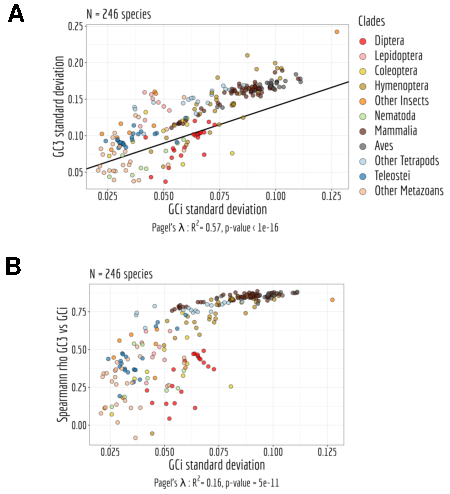
\includegraphics[width=\textwidth] {Figure1_supp.pdf}
    \end{center}                                                                       
    \caption[Transcriptome sequencing depth affects intron detection power and AS rate estimates]{\textbf{Transcriptome sequencing depth affects intron detection power and AS rate estimates.} To assess the impact of sequencing depth on AS detection, we conducted a pilot analysis with two species (\textbf{A,C}: \textit{Homo sapiens} and \textbf{B,D}: \textit{Drosophila melanogaster}) for which hundreds of RNA-seq samples are available (\hyperref[table:1]{Supplementary Tab. 1}; refer to Data10-supp.tab in the Zenodo data repository). We randomly drew 1 to 20 RNA-seq samples and, for each draw, we computed the median read coverage across BUSCO gene exons (to get a measure of transcriptome sequencing depth that is comparable across species). We also computed for each draw the average AS rate and the fraction of introns supported by at least 10 RNA-seq reads, out of all introns annotated for BUSCO genes (\nameref{sec:MaterialsMethodsAS}). We repeated this procedure 30 times. As expected, the fraction of BUSCO introns that are supported by at least 10 reads (\textit{i.e.} $\mathrm{N_s+N_a}\geq10$) increases with sequencing depth (\textbf{A,B}). More importantly, we observed that when sequencing depth is limited, the mean AS rate of BUSCO introns is very variable across draws (\textbf{C,D}). However, AS rate estimates converge when sequencing depth exceeds 200. We therefore kept for further analysis those species for which the median read coverage across exonic regions of BUSCO genes was above this threshold.}
    \label{supp_fig:AS1}
\end{figure}
    

\begin{figure}[t]   
    \begin{center}                                                                       
        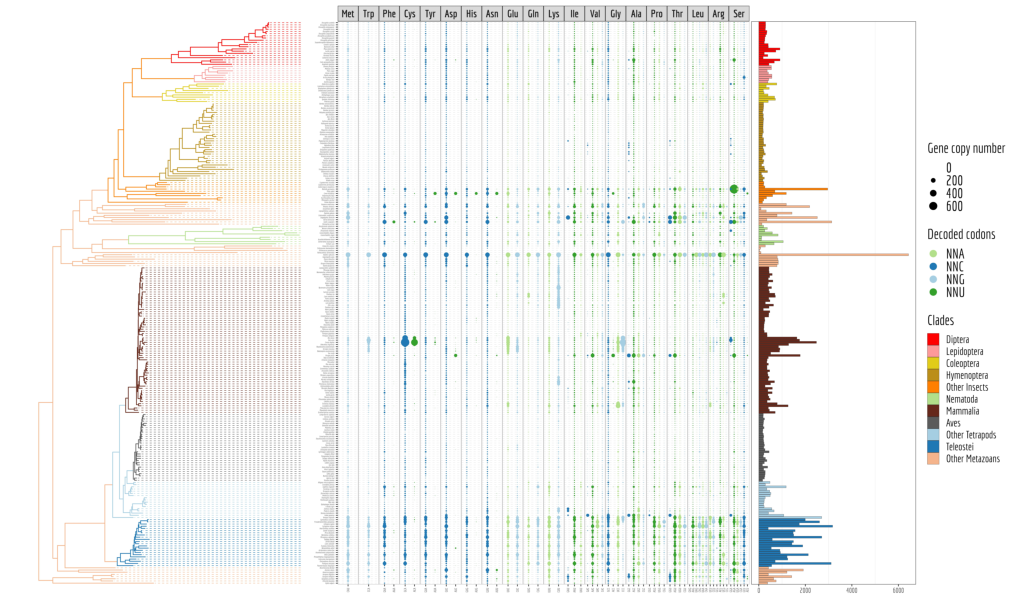
\includegraphics[width=\textwidth] {Figure2_supp.pdf}
    \end{center}                                                                       
    \caption[The power to detect AS events is positively correlated with transcriptome sequencing depth]{\textbf{The power to detect AS events is positively correlated with transcriptome sequencing depth.} Relationship between the proportion of major-isoform introns that have at least one read corresponding to splice variants (\textit{i.e.} $\mathrm{N_a}$ $>$ 0; see Fig. 2), and the median per-base read coverage computed on BUSCO gene exons, across metazoans. Each dot represents one species, colored by taxonomic clade.} 
    \label{supp_fig:AS2}
\end{figure}


\begin{figure}[t]   
    \begin{center}                                                                       
        \includegraphics[width=0.8\textwidth] {Figure3_supp.pdf}
    \end{center}                                                                       
    \caption[Relationship between AS rates and other \textit{N}$_{\text{e}}$ proxies]{\textbf{Relationship between AS rates and other \textit{N}$_{\text{e}}$ proxies.} \textbf{A,B}: Correlation between the average AS rate \textit{per} intron and the body length of each species (cm, log scale) (\textbf{A}) or the ${dN}/{dS}$ ratio on terminal branches of the phylogenetic tree (\textbf{B}). \textbf{C,D,E,F}: Relationship between the average AS rate \textit{per} intron and the body length (cm, log scale) (\textbf{C,E}) or the ${dN}/{dS}$ ratio (\textbf{D,F}). \textbf{C,D}: Low-AS major-isoform introns (\textit{i.e.} major-isoform introns that do not have any abundant SV). \textbf{E,F}: High-AS major-isoform introns (\textit{i.e.} major-isoform introns having at least one abundant SV). Only BUSCO genes were used in the analysis.}
    \label{supp_fig:AS3}
\end{figure}


\clearpage

\begin{figure}[t]   
    \begin{center}                                                                       
        \includegraphics[width=\textwidth] {Figure4_supp.pdf}
    \end{center}                                                                       
    \caption[The rate of alternative splicing correlates with life history traits in both vertebrates and insects]{
     \textbf{The rate of alternative splicing correlates with life history traits in both vertebrates and insects.} Correlation between the average AS rate per intron and longevity of each species (days, log scale) (\textbf{A,B}), body length (cm, log scale) (\textbf{B,E}), or the dN/dS ratio on terminal branches of the phylogenetic tree (\textbf{C,F}). In vertebrates (\textbf{A,B,C}) and insects 
 \textbf{C,D,E}). Only the BUSCO genes were included in the analysis.}
    \label{supp_fig:AS4}
\end{figure}


\begin{figure}[t]   
    \begin{center}                                                                       
        \includegraphics {Figure5_supp.pdf}
    \end{center}                                                                       
    \caption[The variation in AS rates between species is not explained by organ differences]{\textbf{The variation in AS rates between species is not explained by organ differences.} Variation in average AS rate across seven organs (brain, cerebellum, heart, liver, kidney, testis, and ovary) among seven vertebrate species (RNA-seq data from~\citet{cardoso-moreira_gene_2019}) and across three organs (ovary, testis, and head) for one insect (\textit{Dendroctonus ponderosae}, Coleoptera). AS rates were computed for the major-isoform introns from BUSCO genes (\nameref{sec:MaterialsMethodsAS}).} 
    \label{supp_fig:AS5}
\end{figure}


\begin{figure}[t]   
    \begin{center}                                                                       
        \includegraphics {Figure6_supp.pdf}
    \end{center}
    \caption[SNP density in human splice signals, for dinucleotides affected by CpG hypermutability]{\textbf{SNP density in human splice signals, for dinucleotides affected by CpG hypermutability.} Density of SNPs on splice signals for major-isoform introns and for SVs that have their  minor splice site within the adjacent exon or in the major-isoform intron. The number of introns studied is shown at the top of each bar. \textbf{A,B}: SNP data from the human 1000 Genomes project \citep{auton_global_2015}. We included only dinucleotides affected by CpG hypermutability (\nameref{sec:MaterialsMethodsAS}). Error bars represent the 95\% confidence interval of the proportion of polymorphic sites (proportion test). \textbf{A}: Abundant SVs (MIRA $>$ 5\%). \textbf{B}: Rare SVs (MIRA $\leq$ 5\%). \textit{green}: major splice sites; \textit{red}: minor splice sites; \textit{blue}: control dinucleotides.
    }
    \label{supp_fig:AS6}
\end{figure}

\begin{figure}[t]   
    \begin{center}                                                                       
        \includegraphics[width=\textwidth] {Figure7_supp.pdf}
    \end{center}                                                                       
    \caption[Correlations between gene expression levels and AS rates differ among species]{\textbf{Correlations between gene expression levels and AS rates differ among species.} \textbf{A,B}: Relationship between the average AS rate of major-isoform introns (with $\mathrm{N_s+N_a}\geq100$, see \hyperref[fig:AS2]{Fig. 2}) and the expression levels of the corresponding genes (FPKM, log scale). We divided major-isoform introns into 5\% bins according to the expression level of the corresponding genes and computed for each bin the average AS rate and the median expression level. Error bars represent the standard error of the mean. \textbf{A}: \textit{Homo sapiens}, \textbf{B}: \textit{Drosophila melanogaster}. This analysis was performed on all protein-coding genes (\textit{blue}) and BUSCO genes (\textit{light blue}). Pearson correlation presented here was computed on protein-coding genes.}
    \label{supp_fig:AS7}
\end{figure}


\begin{figure}[t]   
    \begin{center}                                                                       
        \includegraphics[width=\textwidth] {Figure8_supp.pdf}
    \end{center}                                                                       
    \caption[Relationship between AS rates and \textit{N}$_{\text{e}}$ proxies, for all major-isoform introns, low-AS major-isoform introns (\textit{i.e.} major-isoform introns that do not have any abundant spliced variants) and high-AS major-isoform introns (\textit{i.e.} major-isoform introns having at least one abundant spliced variants).]{\textbf{Relationship between AS rates and \textit{N}$_{\text{e}}$ proxies, for all major-isoform introns, low-AS major-isoform introns (\textit{i.e.} major-isoform introns that do not have any abundant spliced variants) and high-AS major-isoform introns (\textit{i.e.} major-isoform introns having at least one abundant spliced variants).} Relationship between the average AS rate of all major-isoform introns (\textbf{A,B,C}) or low-AS major-isoform introns (\textbf{D,E,F}) or high-AS major-isoform introns (\textbf{G,H,I}) and longevity (days, log scale) (\textbf{A,D,G}) or body length (cm, log scale) (\textbf{B,E,H}) or the ${dN}/{dS}$ ratio (\textbf{C,F,I}).} 
    \label{supp_fig:AS8}
\end{figure}

\begin{figure}[t]   
    \begin{center}                                                                       
        \includegraphics[width=\textwidth] {Figure9_supp.pdf}
    \end{center}                                                                       
    \caption[Relationship between the proportion of frame-preserving SVs and \textit{N}$_{\text{e}}$ proxies]{\textbf{Relationship between the proportion of frame-preserving SVs and \textit{N}$_{\text{e}}$ proxies.} \textbf{A,B}: Relationship between the proportion of frame-preserving SVs among abundant SVs, and the body length (cm, log scale) of the organism (\textbf{A}) or the ${dN}/{dS}$ ratio (\textbf{B}). Each dot represents one species. All protein-coding genes were used in the analysis.}
    \label{supp_fig:AS9}
\end{figure}


\begin{figure}[t]   
    \begin{center}                                                                       
        \includegraphics[width=\textwidth] {Figure10_supp.pdf}
    \end{center}                                                                       
    \caption[The \textit{per}-gene AS rate is negatively correlated with \textit{N}$_{\text{e}}$]{\textbf{The \textit{per}-gene AS rate is negatively correlated with \textit{N}$_{\text{e}}$.} Relationship between \textit{per}-gene average AS rates and \textit{N}$_{\text{e}}$ proxies. We use as inverse \textit{N}$_{\text{e}}$ proxies the longevity (days, log scale) (\textbf{A,D}) or the body length (cm, log scale) (\textbf{B,E}) or the ${dN}/{dS}$ ratio (\textbf{C,F}). The analysis was done on BUSCO genes (\textbf{A,B,C}) and on all protein-coding genes (\textbf{D,E,F}).}
    \label{supp_fig:AS10}
\end{figure}

\begin{figure}[t]   
    \begin{center}                                                                       
        \includegraphics[width=\textwidth] {Figure11_supp.pdf}
    \end{center}                                                                       
    \caption[Description of the bioinformatic analyses pipeline]{\textbf{Description of the bioinformatic analyses pipeline.} First, we retrieved genomic sequences and annotations from the NCBI Genomes database. We aligned RNA-seq reads with HISAT2 on the corresponding reference genomes, to analyze various variables (see \hyperref[fig:AS2]{Fig. 2}), to compute the AS rate, and to estimate gene expression using Cufflinks. To compute ${dN}/{dS}$, we first identified BUSCO genes with BUSCOv3 and aligned their coding sequences (CDS) using PRANK (codon model). We reconstructed a phylogenetic tree using RAxML-NG with 461 multiple alignments. Using bio++, we estimated ${dN}/{dS}$ along the phylogenetic tree on concatenated alignments.} 
    \label{supp_fig:AS11}
\end{figure}

    \adjustmtc[0]
    

\chapter{Supplementary data and figures Chapter 7}\raggedleft\textcolor{BLUEROYAL}{\LARGE{Why is selection for translationally optimal codons so scarce in metazoans?}}\\
\raggedleft\textcolor{BLUEROYAL}{\Large{Variation in fitness effects and drift intensity}}

{\hypersetup{linkcolor=GREYDARK}\minilof\newpage}

\graphicspath{{chap7-Translational Selection/figures/}}

\raggedright
\textbf{Estimating the strength of selection on synonymous codon usage using population genetics.}
\\
The frequency of optimal codons ($FOP$) reflects the balance between the optimal to non-optimal codons synonymous substitution rate ($K_{on}$) and the non-optimal to optimal codons synonymous substitution rate ($K_{no}$):

\[\text{Non-optimal codon } \autorightleftharpoons{$K_{no}$}{$K_{on}$} \text{ Optimal codon}\]

Substitution rates depend on the corresponding mutation rates ($\mu_{no}$, $\mu_{on}$) and fixation probabilities ($P_{no}$, $P_{on}$): \(K_{no} = 2\textit{N}_{\text{e}} \mu_{no} P_{no}\text{    and    }K_{on} = 2\textit{N}_{\text{e}} \mu_{on} P_{on}\), where \textit{N}$_{\text{e}}$ is the effective population size.

Fixation probabilities are given by:

\[P_{no} =  \frac{1 - e^{-4 \textit{N}_{\text{e}} f_0 s }}{1 - e^{-4 \textit{N}_{\text{e}} s }} = \frac{1 - e^{-2 s }}{1 - e^{-4 \textit{N}_{\text{e}} s }} \stackrel{\text{$s \rightarrow 0$}}{=} \frac{2 s }{1 - e^{-4 \textit{N}_{\text{e}} s }} \text{ similarly } P_{on} \stackrel{\text{$s \rightarrow 0$}}{=} \frac{-2 s }{1 - e^{4 \textit{N}_{\text{e}} s }}  \]


% \[\acrshort{K} = 2\acrshort{Ne}~\acrshort{mu}~P^F = 2\acrshort{Ne}~\acrshort{mu}~\frac{1 - e^{-4\acrshort{Ne}\acrshort{s} p}}{1 - e^{-4\acrshort{Ne}\acrshort{s}}} = 2\acrshort{Ne}~\acrshort{mu}~\frac{1 - e^{-2s}}{1 - e^{-4\acrshort{Ne}\acrshort{s}}}\]

Where $s$ is the selection coefficient in favor of optimal codons and $f_0$ the allele frequency of a new arrival mutation ($f_0 = 1/2\textit{N}_{\text{e}}$).

At equilibrium, the frequency of optimal codons is given by: \(FOP =  \frac{K_{no}}{K_{on} + K_{no}}\)

which can be written as:

\[FOP =  \frac{2 \textit{N}_{\text{e}} \mu_{no} P_{no}}{2 \textit{N}_{\text{e}} \mu_{no} P_{no}+2 \textit{N}_{\text{e}} \mu_{on} P_{on}}
=  \frac{\mu_{no} P_{no}}{\mu_{no} P_{no}+ \mu_{on} P_{on}} =  \frac{\frac{\mu_{no}}{\mu_{on}}  \frac{2s}{1 - e^{-4 \textit{N}_{\text{e}} s} }}{\frac{\mu_{no}}{\mu_{on}}  \frac{2s}{1 - e^{-4 \textit{N}_{\text{e}} s} } + \frac{-2s}{1 - e^{4 \textit{N}_{\text{e}} s} } }
\]

Let us note lambda, the ratio of mutation rates: $\lambda = \frac{\mu_{no}}{\mu_{on}}$

\[FOP =  \frac{\lambda}{\lambda + \frac{-(1 - e^{-4 \textit{N}_{\text{e}} s})}{1 - e^{4 \textit{N}_{\text{e}} s}}}
\]

\[\frac{1}{FOP} = 1 +   \frac{1}{\lambda} \times \frac{-(1 - e^{-4 \textit{N}_{\text{e}} s})}{1 - e^{4 \textit{N}_{\text{e}} s}}
\]

\[\frac{1}{FOP} - 1 =   \frac{-(1 - e^{-4 \textit{N}_{\text{e}} s})}{1 - e^{4 \textit{N}_{\text{e}} s}} \times \frac{1}{\lambda} 
\]

\[\frac{1-FOP}{FOP} \times \lambda = \frac{-(1 - e^{-4 \textit{N}_{\text{e}} s})}{1 - e^{4 \textit{N}_{\text{e}} s}} 
\]

\setcounter{equation}{0}
\begin{equation}
\frac{FOP}{1-FOP} \times \frac{1}{\lambda}  = \frac{1 - e^{4 \textit{N}_{\text{e}} s}}{-(1 - e^{-4 \textit{N}_{\text{e}} s})} 
\end{equation}

\newpage

With the following simplification:

\[ \frac{1 - e^{4 \textit{N}_{\text{e}} s}}{-(1 - e^{-4 \textit{N}_{\text{e}} s})} = \frac{1 - e^{4 \textit{N}_{\text{e}} s}}{-(1 - \frac{1}{e^{4 \textit{N}_{\text{e}} s}})} 
 = \frac{e^{4 \textit{N}_{\text{e}} s} \times (1-e^{4 \textit{N}_{\text{e}} s})}{1 - e^{4 \textit{N}_{\text{e}} s}} = e^{4 \textit{N}_{\text{e}} s}
\]

\[ (1) \rightarrow \frac{FOP}{1-FOP} \times \frac{1}{\lambda} = e^{4 \textit{N}_{\text{e}} s}
\]


Thus, the population-scaled selection coefficient ($S=4 \textit{N}_{\text{e}} s$) is given by:

\[ S = log(\frac{FOP}{1-FOP}) - log(\lambda) = logit(FOP) - log(\lambda)
\]

Hence, we expect a linear correlation between logit($FOP$) and $S$:

\[ logit(FOP) = S + log(\lambda)
\]


\setcounter{figure}{0}
\begin{figure*}[htbp]
    \centering                                                                            
    \includegraphics[width=0.8\textwidth]{Figure1_app.pdf}                                               
    \label{appfig:1}
\end{figure*}

\newpage

If for weakly-expressed genes there is no selection, implied by the non-variation of $FOP$ with gene expression, $S^{lx}\approx0$ :

\[ logit(FOP^{lx}) = 0 + log(\lambda)
\]


\[ logit(FOP^{hx}) = S^{hx} + log(\lambda)
\]

\[ S^{hx}  = logit(FOP^{hx}) - logit(FOP^{lx})
\]

\begin{figure*}[htbp]
    \centering                                                                            
    \includegraphics[width=\textwidth]{Figure2_app.pdf}                                               
    \label{appfig:2}
\end{figure*}


\newpage


\begin{figure*}[t]
    \centering                                                                            
    \includegraphics[width=0.6\textwidth]{Figure1_supp.pdf}                                               
    \caption[Intra-species codon usage variations]{\textbf{Intra-species codon usage variations.} \textbf{A}: Relationship between the standard deviation of the \textit{per} gene GC at the third position (GC3) and the GC in introns (GCi). \textbf{B}: Relationship between the Spearman coefficient (rho) reflecting the correlation between GC3 of genes and GC content in introns within a specific species, and the standard deviation of the \textit{per} gene GC in introns.}
    \label{suppfig:CU1}
\end{figure*}


\begin{figure*}[t]
    \centering                                                                            
    \includegraphics[width=\textwidth]{Figure2_supp.pdf}                                   
    \caption[tRNA gene copy number]{\textbf{tRNA gene copy number.} For the 257 studied species from left to right: phylogenetic tree, number of tRNA gene copy number \textit{per} amino acid \textit{per} codons and total number of tRNA gene copy.} 
    \label{suppfig:CU2}
\end{figure*}


\begin{figure*}[t]
    \centering                                                                            
    \includegraphics[width=\textwidth]{Figure3_supp.pdf}                                   
    \caption[tRNA abundance proxies]{\textbf{tRNA abundance proxies.} \textbf{A,B}: Relationship between the tRNA abundance measured by~\citet{behrens_high-resolution_2021} and the frequency of amino acid weighted by gene expression (FPKM). \textbf{C,D}: Relationship between tRNA gene copy number and the frequency of amino acid weighted by gene expression (FPKM). Left: \textit{Drosophila melanogaster}; Right: \textit{Homo sapiens}} 
    \label{suppfig:CU3}
\end{figure*}

\begin{figure*}[t]   
    \begin{center}                                                                       
        \includegraphics[width=\textwidth]{Figure5_supp.pdf}
    \end{center}                                                                       
    \caption[Counting for intronic background do not change the signal of translational selection]{\textbf{Counting for intronic background do not change the signal of translational selection.} The X-axis represents variations in POCs frequency, calculated as the difference between POC frequency in the 2\% most highly expressed genes and the 50\% least expressed genes. The Y-axis depicts the refined X-axis values by eliminating variations arising from non-adaptive processes, such as the difference in POC-control frequency between the 2\% most highly expressed genes and the 50\% least expressed genes. The black line represents the pagel's \textit{lambda} model, and the dotted line represents x=y.} 
    \label{suppfig:CU5}
\end{figure*}


\begin{figure*}[t]   
    \begin{center}                                                                       
        \includegraphics[width=\textwidth]{Figure6_supp.pdf}
    \end{center}                                                                       
    \caption[Non homogenous GC composition along genes]{\textbf{Non homogenous GC composition along genes.} \textbf{A,B}: Measured of the GC composition in introns using 100 bp windows from the start codon and the stop codon (kb, log scale). Equal group of genes have been formed regarding their length, represented by distinct color groups. \textbf{A}: \textit{Homo sapiens}; \textbf{B}: \textit{Drosophila melanogaster}} 
    \label{suppfig:CU6}
\end{figure*}


\begin{figure*}[t]
    \centering                                                                            
    \includegraphics[width=\textwidth]{Figure7_supp.pdf}
    \caption[Non homogenous GC composition along genes for 11 clades]{\textbf{Non homogenous GC composition along genes for 11 clades.} Measured of the GC composition in introns using 100 bp windows from the start codon and the stop codon (kb, log scale). Each clade of the study is represented by color, one line represents one species.} 
    \label{suppfig:CU7}
\end{figure*}


\begin{figure*}[t]
    \centering                                                                            
    \includegraphics[width=\textwidth]{Figure8_supp.pdf}
    \caption[Multiple genome alignment quality of \textit{Drosophila simulans} and \textit{Drosophila erecta} on \textit{Drosophila melanogaster}]{\textbf{Multiple genome alignment quality of \textit{Drosophila simulans} and \textit{Drosophila erecta} on \textit{Drosophila melanogaster}.} 
    On the genome of \textit{Drosophila melanogaster} we quantify the fraction of sites mapped to the two other genomes, and the similarity of these sites. The red dotted lines represent the threshold above or below which the quality of the multiple genome alignment is poor.} 
    \label{suppfig:CU8}
\end{figure*}

\begin{figure*}[t]
    \centering                                                                            
    \includegraphics[width=\textwidth]{Figure9_supp.pdf}
    \caption[Differences in usage of putative-optimal codon between highly- and lowly-expressed genes in 6 species]{\textbf{Differences in usage of putative-optimal codon between highly- and lowly-expressed genes in 6 species.} Variation in the proportion of POC within coding sequences (POC1: dark blue; POC2: dark green) according to gene expression level. To control for variations in neutral substitution patterns, we analyzed the frequency of corresponding triplets within introns (POC1 control: light blue; POC2 control: light green). Each point represents a 2\% bin of genes, with the red point at the end of each POC1 curve denoting the 2\% most highly expressed genes. The red lines indicate the average POC1 proportions observed in the 50\% least expressed genes (FPKM, log scale).} 
    \label{suppfig:CU9}
\end{figure*}



\begin{figure*}[t]
    \centering                                                                            
    \includegraphics[width=\textwidth]{Figure10_supp.pdf}
    \caption[Relationship between \textit{N}$_{\text{e}}$ and its proxies]{\textbf{Relationship between \textit{N}$_{\text{e}}$ and its proxies.} Relationship between \textit{N}$_{\text{e}}$ and the longevity (days, log scale; \textbf{A}), body length (cm, log scale; \textbf{B}), body mass (kg, log scale; \textbf{C}), dN/dS (log scale; \textbf{D}). Pagel's \textit{lambda} model is used to take into account the phylogenetic structure of the data in a regression model (the regression line is displayed in black when the correlation is significant). } 
    \label{suppfig:CU10}
\end{figure*}
  

    
\begin{figure*}[t]
    \centering                                                                            
    \includegraphics[width=\textwidth]{Figure11_supp.pdf}
    \caption[Valine synonymous codons usage variations with expression among 4 species]{\textbf{Valine synonymous codons usage variations with expression among 4 species.} Relationship between the relative synonymous codon usage (RSCU) of valine synonymous codons (GTG/GTA/GTT/GTC) and gene expression in four species with different GC richness.} 
    \label{suppfig:CU11}
\end{figure*}


\begin{figure*}[t]
    \centering                                                                            
    \includegraphics[width=\textwidth]{Figure12_supp.pdf}
    \caption[Presence-Absence of tRNA defines set of putative-optimal codons for species subject to translational selection]{\textbf{Presence-Absence of tRNA defines set of putative-optimal codons for species subject to translational selection.} \textbf{A}: Illustration of the various possible pairings: Watson-Crick and wobble pairing. \textbf{B}: A boxplot illustrating the distribution of tRNA gene copy numbers across 26 species subject to translational selection (Lepidoptera and Diptera). The percentage of species lacking a tRNA gene copy is also indicated, highlighting the absence of tRNA isodecoder.} 
    \label{suppfig:CU12}
\end{figure*}

    
    % \myemptypage
    
    
\chapter{Preliminary results}

{\hypersetup{linkcolor=GREYDARK}\minilof\newpage}

\graphicspath{{chap7-Translational Selection/figures/}}


\begin{figure}[t]
    \centering                                                                            
    \includegraphics[width=\textwidth] {figures/Appen_C1.pdf}                                               
    \caption[Translational selection in Diptera]{\textbf{Translational selection in Diptera.} \textbf{A}: Number of genes with reciprocal blast hits with \textit{D. melanogaster} for 95 dipterans, and phylogenetic distance from \textit{D. melanogaster}. \textbf{B}: Gene expression measured in \textit{Z. cucurbitae} compared to the gene expression measured in \textit{D. melanogaster} for genes with reciprocal blast hits. \textbf{C}: Spearmann coefficient (rho), corresponding to the graphic in \textbf{B}, for 22 species for which gene expression data were available. X-axis is the phylogenetic distance from \textit{D. melanogaster}. \textbf{D}: Relationship between GC3 and GCi for the 95 dipterans studied. \textbf{F}: Relationship between the GC3 of codons optimizing translation and GCi for the 95 dipterans studied.}
    \label{suppfig:AppC1}
\end{figure}


\begin{figure}[t]
    \centering                                                                            
    \includegraphics[width=\textwidth] {figures/Appen_C2.pdf}                                   
     \caption[Impact of \Ne~on introns length and genomes size]{\textbf{Impact of \Ne~on introns length and genomes size.} \textbf{A}: Relationship between median intron length and longevity (days, log scale) per species from GTDrift. \textbf{B}: Relationship between median intron length and longevity (days, log scale) focused on hymenopterans. \textbf{C}: Relationship between genomes size (Mb) and longevity (days, log scale). \textbf{D}: Relationship between genomes size (Mb) and longevity (days, log scale) focused on hymenopterans. 
     Pagel's \textit{lambda} model is used to take into account the phylogenetic structure of the data in a regression model (black line if significant).} 
    \label{suppfig:AppC2}
\end{figure}
    
    
%%%%% REFERENCES
    
    
    \myemptypage
    
    \bibliographystyle{natbib}
    \bibliography{references}
\end{document}

